%---[ TEMPLATE: BOOK | monograph ]
%---|original-author:JWL|date:21AUG2025|email:jwl@nuchwezi.com
%---|TITLE: Applying TRANSFORMATICS in GENETICS
%----------------------------------------------------------------|
%\documentclass[a4paper, 18pt]{article} % A4 paper, readable font size
\documentclass[a4paper, 18pt]{book} % A4 paper, readable font size
%\documentclass[a4paper, 18pt]{book} % A4 paper, readable font size
\usepackage{geometry} % Adjust margins
\geometry{top=0.8in, bottom=0.8in, left=0.8in, right=0.6in} 


% packages we'll need...

% allow table of contents to also list subsections
\setcounter{tocdepth}{2}

% for better appendices
\usepackage[title,titletoc]{appendix}

% for controlling page numbers
\usepackage{fancyhdr}
\pagestyle{fancy}
\fancyhf{}
\fancyhead[R]{\thepage}

% throw in page-top header
\fancyhead[L]{Applying \textbf{TRANSFORMATICS} in GENETICS}

% for graphics
\usepackage{graphicx}
\usepackage{caption}
\usepackage{float}

% for text-wrapping in verbatim environments
\usepackage{fvextra}
\RecustomVerbatimEnvironment{verbatim}{Verbatim}{breaklines, breakanywhere}

% for drawing text boxes

% for proper treatment of urls
\usepackage{hyperref}

% for tables
\usepackage{tabularx}

% for line-breaks in table cells
\usepackage{makecell}

% for diagonalsplit in table headers cell
\usepackage{diagbox}

% make table cells center vertically where we could have used p{1cm} -- we use m{1cm}
%\usepackage{array}
% alternatively, just use custom column type --- M{1cm}
%\newcolumntype{M}[1]{>{\centering\arraybackslash}m{#1}}


% for long tables
\usepackage{longtable}
% for custom table col widths
%\usepackage{array}
%\newcolumntype{L}{>{\centering\arraybackslash}m{2cm}}
%\newcolumntype{M}{>{\centering\arraybackslash}m{5cm}}

% for json listings...
\usepackage{listings}
%\usepackage{minted}
%\usemintedstyle{xcode}% no parser errors in listings?
%\usemintedstyle{bw} % grayscale color in listings, but shows parser errors!

% for maths
\usepackage{amsmath}
% for number sets symbols
\usepackage{amssymb}
%\usepackage{ntheorem}
\usepackage{amsthm}

\usepackage{tikz} % for v-aligned matrices with arrows between them
\usetikzlibrary{matrix, positioning} % ← This line is essential


% extra symbols
\usepackage{textgreek}
%\usepackage{mnsymbol}

% for writing our theorems and defs...
\newtheorem{comp}{Computation}
\newtheorem{theo}{Theorem}
\newtheorem{defn}{Definition}
\newtheorem{lem}{Lemma}
\newtheorem{prop}{Proposition}
\newtheorem{axiom}{Axiom}
\newtheorem{post}{Postulate}
\newtheorem{trans}{Transformation}
\newtheorem{transf}{Transformer}
\newtheorem{law}{Law}
\newtheorem{prob}{Problem}
\newtheorem{soln}{Solution}
\newtheorem{alg}{Algorithm}

% for highlighting text
\usepackage{xcolor, soul}
\definecolor{highcolor}{rgb}{0,255,255} %a color for background, that is friendly on black text foreground
\sethlcolor{highcolor}


% for wrapping text around floats
\usepackage{wrapfig}

% to include pdf pages
\usepackage{pdfpages}

% for multiline comments...
\newcommand{\comment}[1]{}

% for the cardinality symbol
\newcommand{\invpi}{\rotatebox[origin=c]{180}{$\pi$}}

\title{Applying \textbf{TRANSFORMATICS} in GENETICS}


\author{Willrich J. Lutalo\thanks{Currently a volunteering \& Independent Principal Investigator at Nuchwezi Research --- \url{https://nuchwezi.com}}\\
\texttt{joewillrich@gmail.com, jwl@nuchwezi.com}}

\date{21$^{st}$ August, 2025}


\begin{document}

%---[ START BOOK CONTENT/FRONT ]
\frontmatter

% insert [front] cover --- could just be a PNG or PDF
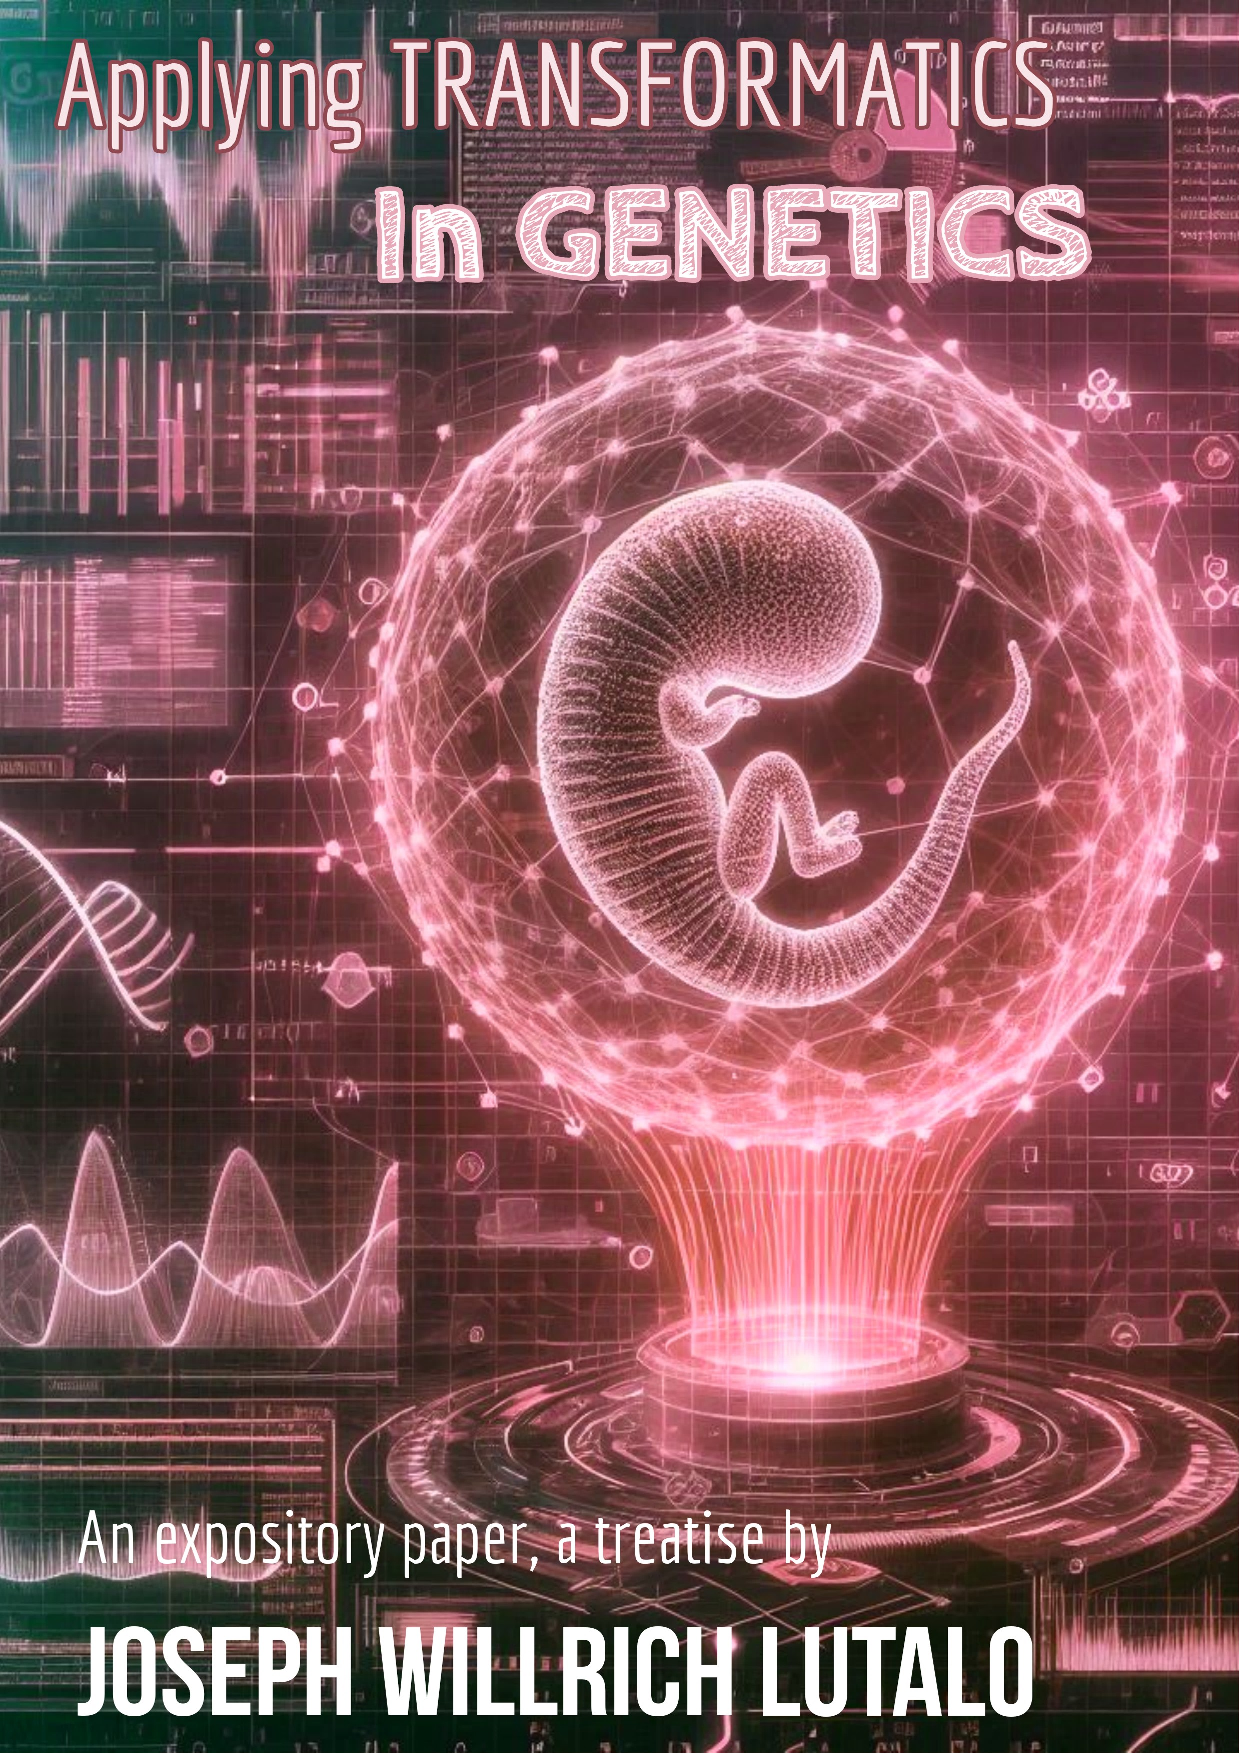
\includepdf[pages=1]{resources/pdfs/front_cover.pdf}


% insert I*POW frontmatter
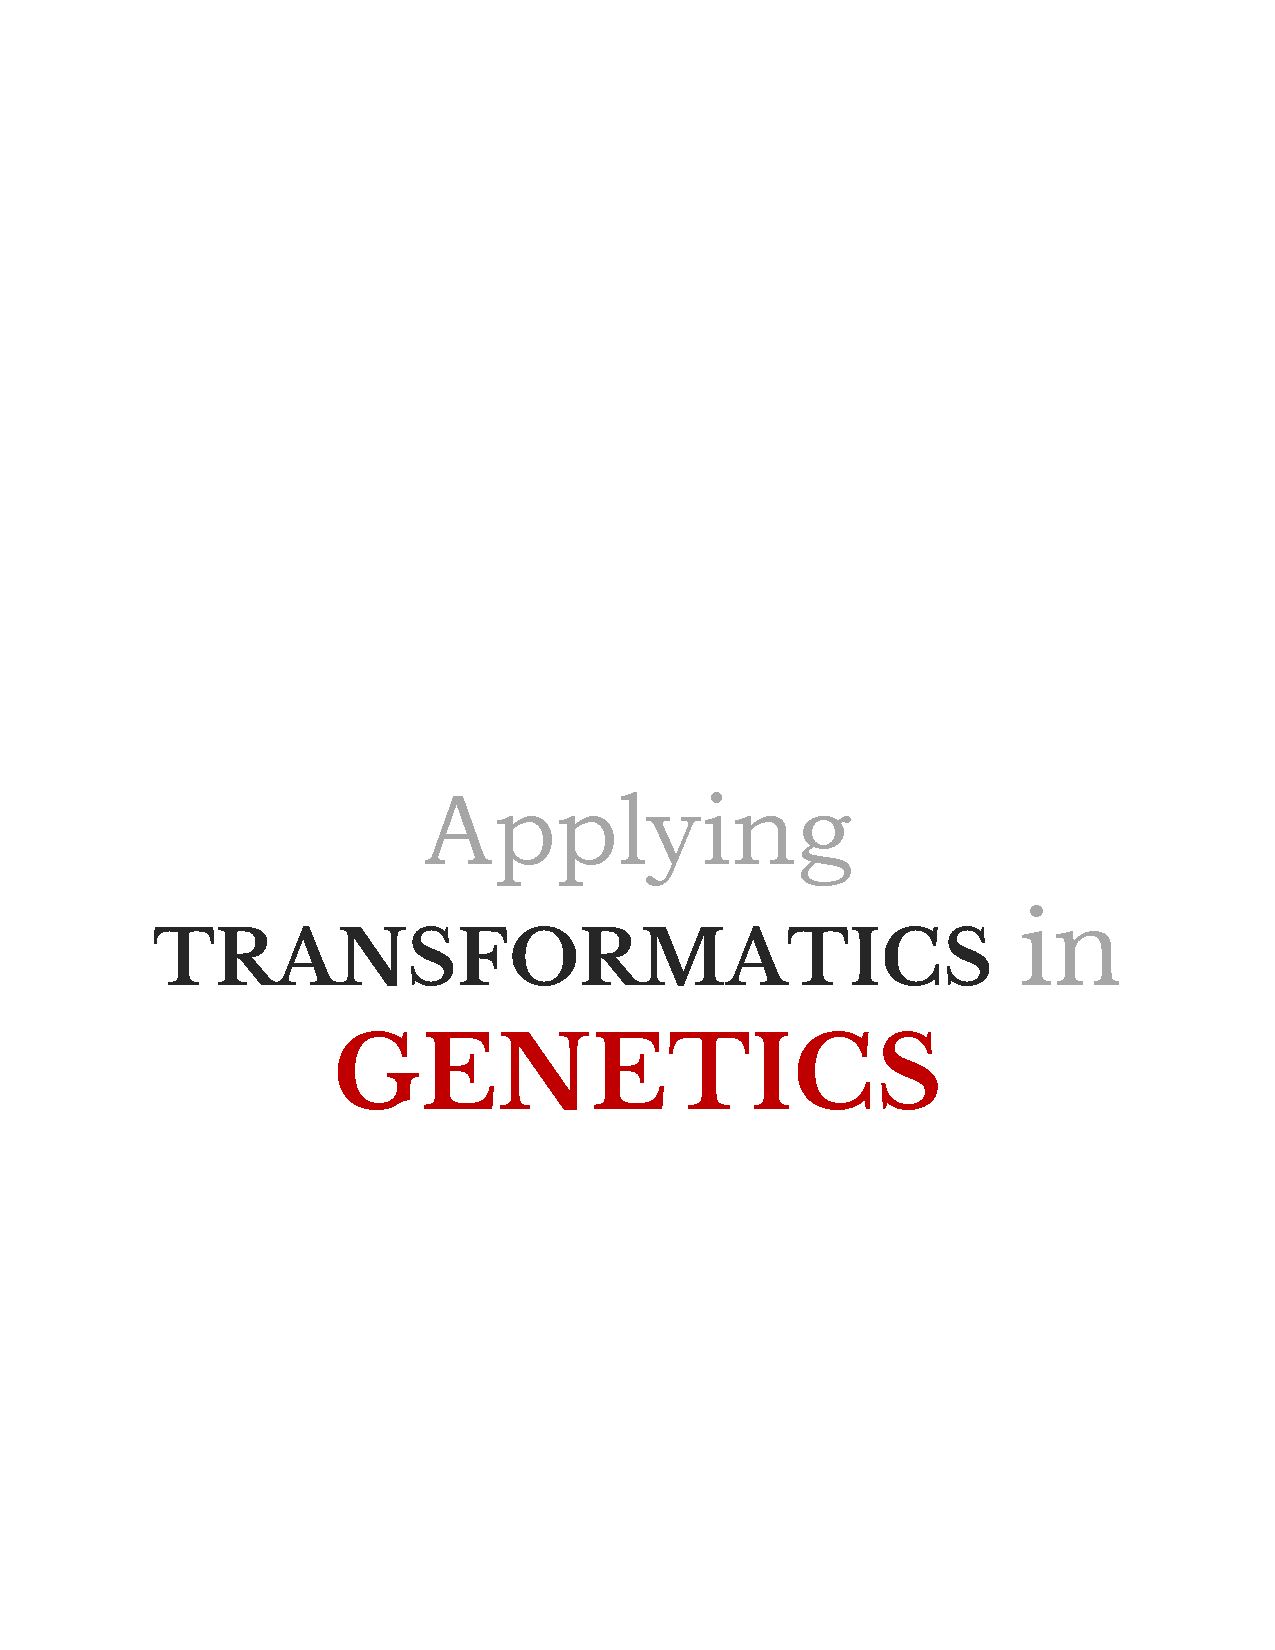
\includepdf[pages=-]{resources/pdfs/FrontisMatter.pdf}



\maketitle

\chapter*{Dedication}


\begin{table}[H]
  \centering
  \Huge
	\begin{tabular}[t]{|p{0.8\textwidth}}
The friendly, 20th century philosopher, \textbf{Alan Watts}, \small such a fatherly, enlightening voice I keep hearing in my thoughts every once in a while; for I enjoy listening to his rants, once said \Huge \textit{``You are the universe experiencing itself."} \Large I always wished to be a father to someone... \textbf{a real boy or a girl out there... a soul... my own genetic code alive and existing independently of me}. To experience and enjoy the expressions of my own genetic code remains among my greatest dreams. But, in case I don't see my own child in this lifetime, at least, this message should inspire those that read it, who come after, to know and trust that when we express ourselves, we in a way express those that brought us into the world. Personally, I would cherish it! I surely dedicate this work to you, my father and mother. \Large I can't express enough how grateful I am, that you enabled me to be... You gave me a distinctive identity and a voice. \Huge \textbf{May this work help further your expressions in this world... and beyond.}\\
	\hline
	              
\end{tabular}
  \label{TABDEDC}
\end{table}

\tableofcontents

\listoffigures

\listoftables

\newpage

\Large


\chapter{Preface}

\begin{quotation}
\noindent \texttt{Jung restored the colour in science, and made me cherish the mind in new ways...}\\
\texttt{And that in exercising our will we might become aware of the divine in us and thus make glory manifest. God is not asleep in us!}\\
\hspace*{\fill} --- \textbf{J. Willrich Lutalo}, \textit{Shrines of The Free Men}, 2018\cite{shrinesjwl}
\end{quotation}

We are living in a world where man affects and influences nature so much, especially with his \textit{unnatural} inventions in the form of animated and inanimate intelligence, implements and reality augmentations. But also, the world around man is constantly changing, and sometimes, in ways other than man is naturally comfortable with. That said, there is this idea that \textit{a life unexplored isn't worth living}\footnote{I trust, it is attributed to ancient philosopher and student of \textbf{Socrates}, Aristocles son of Ariston aka. `Plato'.}, and come what may, with every passing day, and as seasons and times change, it seems like the compulsion for humans to have to leave their traditional home environments and explore life elsewhere --- say, in foreign countries, in/under the sea, \textit{inside} the earth or away from it, say like in outer-space, etc. seems so unavoidable --- in fact, it feels to me like it is inculcated into our very natures, so that, thinking about a future in the same exact space, with the same exact people, environment and/or circumstances as we wake up to every day just doesn't make much sense\footnote{I have read a sane dose of \textbf{Daniel Defoe}'s classic, \textit{The Life and Adventures of Robinson Crusoe}, a relic from 1719, and among things Defoe seemed to argue against, was the somewhat strong urge in some humans, to want to go ``abroad upon Adventures, to rise by Enterprise, and make themselves famous in Undertakings of a Nature out of the common Road".}. That we must prepare ourselves --- ``we", meaning \textit{humans}, to face an uncertain future, but also, to lessen such uncertainty to manageable levels where possible or necessary, is much of what justifies our investments in and explorations of science and knowledge in general. 

For those who trust \textit{divinely inspired} wisdom\footnote{I keep an indispensable copy of \textbf{The New Jerusalem Bible}, and wouldn't wish to do much without consulting it first!}, the sacred scriptures (in \textbf{Genesis 1:28}) empower us thus:

\begin{quotation}
\noindent \texttt{God blessed them, saying to them, \textit{Be \textbf{fruitful, multiply, fill the earth and subdue it}. Be masters of the fish of the sea, the birds of heaven and all the living creatures that move on earth.}}\\
\end{quotation}


Despite not having been funded by any one or any particular organization, the author, passionate about his pursuit of a \textbf{Doctorate in Philosophy} --- of Computer Science or Mathematics, from the \textbf{University of Oxford}\cite{lutalo_2025_sop}\cite{Lutalo2025_phd} or any other reputable institution\footnote{Refer to \textbf{ORCID:} \url{https://orcid.org/0000-0002-0002-4657}}, and especially to secure a teaching or faculty position, somewhere\footnote{Because, in all fairness, knowledge must not only be sought or furthered, but must also be shared.}, embarked on this project, especially to further his earlier work on Transformatics\cite{transformatics} as well as to bring to better audiences, the now stable advances in his original, commercially-viable \textbf{TEA programming language}\cite{cli_tttt}, by exploring new ground, proposing ideas and applications, in a domain potentially more in-demand and with far-reaching consequences for not just humanity, but all of nature, now, tomorrow, and in the deep, far-future. 



% Title for the section
\chapter*{List of Abbreviations}
\addcontentsline{toc}{chapter}{List of Abbreviations}

% Longtable for abbreviation list
\begin{longtable}{p{3cm} p{12cm}}
\textbf{ABBR.} & \textbf{Definition} \\
\hline
\endfirsthead

\textbf{ABBR.} & \textbf{Definition} \\
\hline
\endhead

% Add your abbreviations below
\textbf{ADM} & Anagram Distance Measure \\
\textbf{COS} & Consensus Overlapping Sequence \\
\textbf{DNA} & Deoxyribonucleic Acid \\
\textbf{FGE} & Full Genome Expression \\
\textbf{FLSA} & First Lu-Shuffle Algorithm \\
\textbf{IFA} & Intermediate Form Affix \\
\textbf{I*POW} & International Portfolio of Writers \\
\textbf{IGS} & Identity Genome Sequence \\
\textbf{JSON} & JavaScript Object Notation \\
\textbf{LGES} & Lu-Genome Expression System \\
\textbf{LNS} & Lu-Number System\\
\textbf{MCS} & Maximum Common Subsequence \\
\textbf{\textit{m}RNA} & \textit{messenger}-\textbf{RNA} \\
\textbf{MSS} & Model Sequence Statistic \\
\textbf{\textit{n}-SSI} & \textit{natural}-Symbol Set Identity \\
\textbf{\textit{o}-SSI} & \textit{orthogonal}-Symbol Set Identity \\
\textbf{ORS} & Overlap Resultant Sequence \\
\textbf{PFA} & Platonic Form Aspect \\
\textbf{RNA} & Ribonucleic Acid  \\
\textbf{RNG} & Random Number Generator  \\
\textbf{RPMSS} & Representative Population \textbf{MSS}  \\
\textbf{RSG} & Random Sequence Generator  \\
\textbf{SLSA} & Second Lu-Shuffle Algorithm  \\
\textbf{TEA} & Transforming Executable Alphabet \\
\textbf{\textit{t}RNA} & \textit{transfer}-\textbf{RNA} \\
\textbf{WSL} & Windows Subsystem for Linux\\
\textbf{x-LGES} & Extended \textbf{LGES} \\
\textbf{YAML} & Yet Another Markup Language \\


\end{longtable}




%---[ BEGIN BOOK CONTENT/CHAPTERS ]

\mainmatter

%\begin{abstract}
\chapter*{Abstract}
\large

It started out as just a paper but is now a monograph. \textbf{Applying TRANSFORMATICS in GENETICS} brings to surface the importance of leveraging the mathematical theory recently named ``Transformatics", that deals with the study, processing and analysis of especially ordered sequences of symbols and their transformations via symbolic machines known as sequence transformers. In earlier and recent work by the author, it has been demonstrated to be a credible and powerful theory in designing, specifying and/or explaining the properties of automata operating on sequences to produce other sequences. So, in this particular work, we take that body of knowledge, as well as what we know about the important science of how natural/biological life-forms are defined, transformed and expressed in nature based on genetic code sequences known as DNA (deoxyribonucleic acid), and use that to revisit old and new problems in the field of GENETICS, developing many new, and previously unpresented solutions based on the theories, calculus and mechanics of sequence transformers (aka, ``transformatics"). We have used transformatics to develop, but also distill many useful general results in the form of theorems as well as 3 laws concerning na-Sequences. We have demonstrated how sequence transformers can be leveraged to solve specific or particular practical problems in genetics via numerous well-structured sequence transformations. We have invented and presented several new algorithms that would allow the concepts and solutions we developed in transformatics theory for various general problems to be readily turned into computable solutions using any programming language, for scenarios in genetics, leveraging TEA and Python mostly. We have demonstrated how to leverage statistical analysis to make quantifiable differences and similarities between two or more na-Sequences and/or entire populations of them readily discernible. Leveraging transformatics, we have developed a new theory and systematic framework, the Lu-Genome Expression System, with which, via explorations by eye and hand, but also via the use of computers, the matter of how individual DNA sequences, and generally, any sequence that can be transformed into a numeric/decimal sequence, can be used to explore the natural concept of gene and genome expression, in both a visual-spatial, but also mathematical-symbolic way. We have tackled the fundamentally critical problem of genome sequencing, and have managed to not only cast it rigorously using the language and notions of transformatics, but have also managed to define an abstract machine that can take a set of DNA sequences potentially out of alignment, and then derive from them, via systematic and meaningful alignment procedures, a final, representative consensus genome sequence. Though this work is significantly theoretical and mathematical, we anticipate that the discussions, notes, formulations, solutions and overall expository treatment of the subject that it brings forth, shall help inspire actual domain experts and other researchers interested in genetics, genetic engineering and related sciences to pick up and apply our transformatics theory and ideas in both theory and practice.
     \newline\newline
     \textbf{Keywords}: Mathematical Statistics, Linear Algebra, Transformatics, Artificial Intelligence, Sequence Processors, Sequence Analysis, DNA, Genetic Code, Genetic Analysis, Abstract Machines, Genome Sequencing, Genome Expression, Sequence Programming, Transformers
%\end{abstract}

\newpage

\chapter{Introduction}
\label{SEC1}


\begin{figure}[H]
  \begin{center}
  %\includegraphics[trim=2cm 8cm 2cm 8cm, clip, width=0.9\textwidth,]{resources/pdfs/ProteinSynthesisStateMachine.pdf}\\
   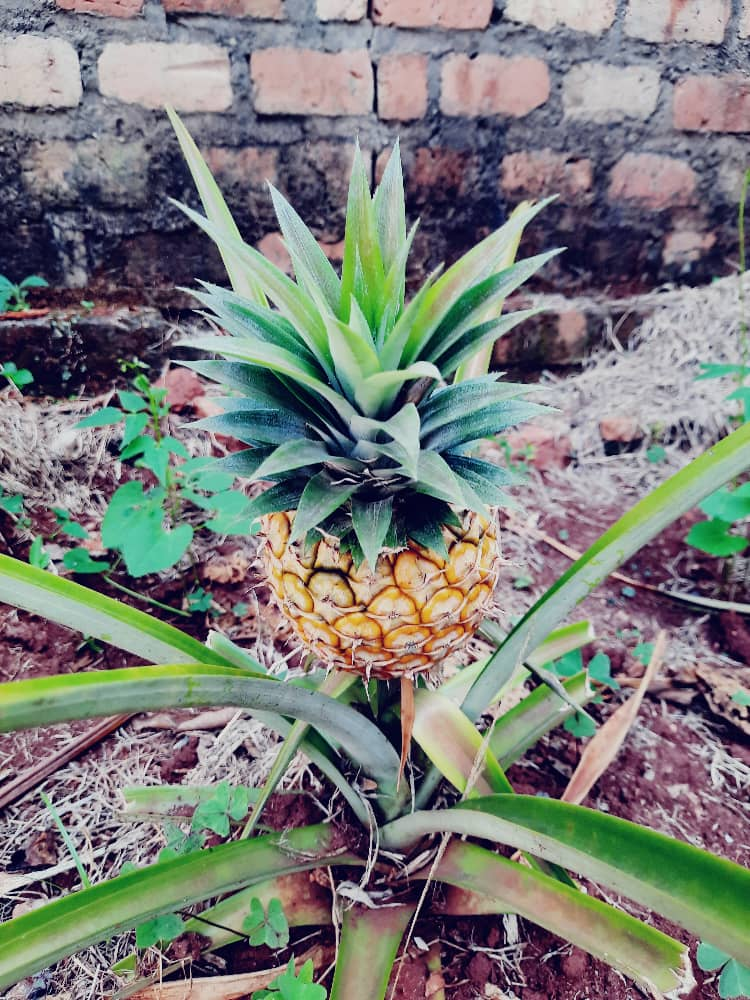
\includegraphics[height=0.6\textheight,]{resources/images/the_pineapple.jpg}\\
   \caption{In the course of writing this work, an experiment to grow pineapples from the pineapple fruit tops of pineapples normally bought from nearby marketplace (\textbf{Garuga/Bugabo-Bukaaya}) yielded results! Here we see the first successful harvest of a pineapple from our home garden (at \textbf{Nuchwezi Research}). But also, this case inspired part of the discussion in \textbf{\hyperref[SEC4]{Chapter \ref{SEC4}}} about how in real genome expression systems, the organism expressed from genetic code somewhat still includes the genetic code in the manifested organism as some kind of affix --- a prefix (in leaves for example) or suffix (roots), from which the original organism (or the same exact genome) might be later reproduced!}
  \label{FIGPINEAPPLE}
  \end{center}
\end{figure}

\begin{quotation}
\noindent \texttt{Sex seems to have been invented around two billion years ago. Before then, new varieties of organisms could arise only from the accumulation of random mutations --- the selection of changes, letter by letter, in the genetic instructions. Evolution must have been agonizingly slow. With the invention of sex, two organisms could exchange whole paragraphs, pages and books of their DNA code, producing new varieties ready for the sieve of selection. Organisms are selected to engage in sex --- the ones that find it uninteresting quickly become extinct. And this is true not only for the microbes of two billion years ago. We humans have a palpable devotion to exchanging segments of DNA today.}\\
\hspace*{\fill} --- \textbf{Carl Sagan}, \textit{COSMOS}, 1981\cite{sagan1981cosmos}
\end{quotation}


\begin{quotation}
\noindent \texttt{The material basis of heredity is DNA, a ladder-like molecule which carries a message in the form of a `four-letter' code, the letters being four chemical bases, each of which may occupy any rung in the ladder.}\\
\hspace*{\fill} --- \textbf{The Oxford Companion to the Mind}\cite{gregory1987oxford}
\end{quotation}


In reality, we find that living, real organisms are influenced by genetics, their environment, bits of randomness and sometimes emergent behaviors that might not be readily captured by strict rules such as the genetic code of life. However, away from all possibilities, and focusing on what can be said of life expression via the genetic code known as DNA (the \textit{deoxyribonucleic acid}) and RNA (\textit{ribonucleic acid}), especially when applied to the vast spectrum of natural organisms on earth --- from basic \textbf{prokaryotes} (single-celled organisms) such as the simple bacteria that actually have no nucleus\cite{bioexplorer2025}, to  \textbf{eukaryotes}; all the way from basic one-cell kinds such as amoeba\cite{kang2017deep} all the way to sophisticated creatures such as oak trees, vultures, dolphins and human beings! Talking of which, it might be important to set clear that though \textbf{viruses} are a kind of life-form\cite{libretexts2025viruses}, and yet, they are neither prokaryotes nor eukaryotes --- especially because, fundamentally, they are merely some genetic code (DNA or RNA) ``enclosed in a protein coat, lacking cell membranes or organelles"\cite{libretexts2025viruses} --- more technically they are \textbf{acellular entities}.

So, if we bring on-board ideas from \textbf{transformatics}\cite{transformatics} --- a new mathematical statistics theory dealing with sequences of symbols or those of named structures and their processing as well as analysis; for example, if we take the concept of leveraging statistical measures to summarize essential properties of sequences such as DNA --- say, with use of the modal sequence statistic (MSS), we find that, independently of, and without needing to first consult or worry about mainstream genetic code analysis or genetic engineering theory and mechanics, that we can say many useful things about genetic code sequences and that we might be able to break new ground or solve some otherwise still intractable problems concerning sequences of genetic code.


\begin{figure}[H]
	\begin{center}
		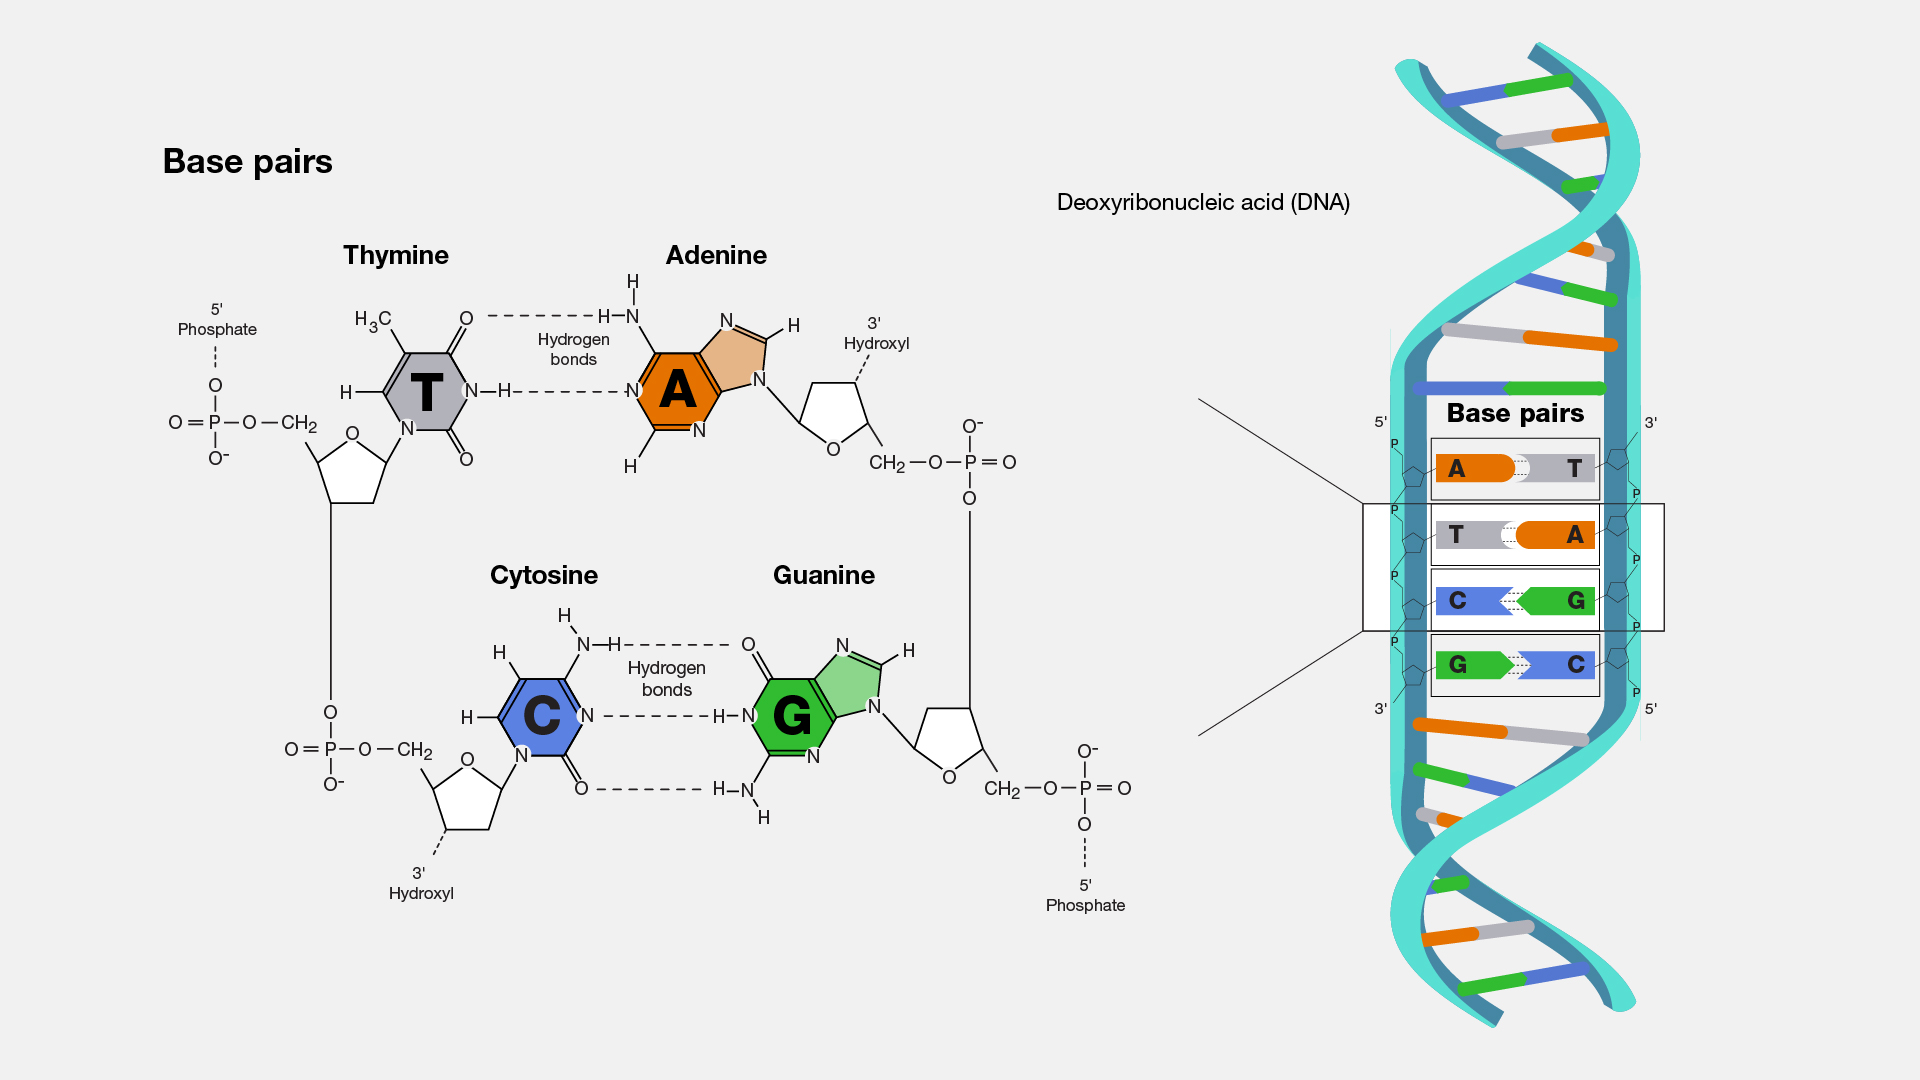
\includegraphics[width=0.9\textwidth]{resources/images/dna_diagram.jpg} \\
		\caption{A basic diagram of the chemical structure of DNA base-pairs from \cite{wikipedia_basepair}}
		\label{FIG1}
\end{center}
\end{figure}
    


For example, by borrowing a useful DNA-as-library metaphor from Venville et al\cite{venville2006analogies}, we would come to appreciate that by looking at \textit{DNA as a library of books}, we have a model such as:

\begin{enumerate}
\item \textbf{Library}: DNA (as a whole) --- the \textbf{Genome},	 as the complete collection of genomic data about an organism.
\item \textbf{Bookshelves}: \textbf{Chromosomes} as organized storage of genes, and that they (chromosomes) are long, coiled-up strands of pairs of genes (essentially, the chromosome is a combination of two strands of genes, with one called the \textit{template} and the other a \textit{complement}, and that when they come together to form the ``ladder" structure, at each step, the two genes forming a step are paired such that $A \leftrightarrow T$ and $C \leftrightarrow G$ \cite{passel_dna_structure} --- also see \textbf{\hyperref[FIG1]{Figure \ref{FIG1}}}). So, for example, humans have 46 chromosomes in total in their ``DNA library" (23 chromosome pairs, consisting of 22 autosomal pairs plus one pair of sex chromosomes). We know that during reproduction, the [full] genome (46 chromosomes in humans) splits up by half in either parent (via \textit{meiosis}, which somewhat shuffles the complete genome and then halves it\cite{genomics2025origin}), so that only one-half of the otherwise well-paired template-complement set that is the chromosome strand from each parent (as either sperm or ovum) goes to contribute to the final chromosome collection-set of the offspring\cite{libretexts2025gametogenesis}\cite{gregory1987oxford}. Whereas, after fertilization or during normal cell division, the entire chromosome set (with well-paired strands) is duplicated/replicated wholesomely and losslessly so that the second/new cell thus created has an exact copy of the same chromosome set (entire genome) as was in the source cell\cite{leicester_cellcycle}. 
\item \textbf{Books}: The \textbf{Genes} which make up a chromosome are the books in our genome library. Each gene is essentially a collection of ``words" that are a sequence of one or more codons (see below), and which taken together, contain enough information/instructions to specify how to produce a specific protein\cite{gregory1987oxford}\cite{venville2006analogies}.
\item \textbf{Words}: And then, at the next, lower abstraction level than genes, we have \textbf{Codons}. These are like ``words" in each book, and each codon \textbf{only} codes for a single \textbf{amino acid}. Basically, a codon is a combination of any 3 of the ``letters" of genetic code, for which, there are exactly four for DNA (A, C, G, T) and four for RNA (A, C, G, U). We also know that there are at most, 64 possible unique combinations of the four letters into triplets/3-grams/the codons\cite{gregory1987oxford}.
\item \textbf{Letters}: Finally, at the most basic level of our genetic code/DNA-library/genome, we have ``letters" that are technically known as \textbf{nucleotides}. Essentially, each nucleotide contains \textbf{a single nucleobase}, with only one difference between DNA and RNA as such; for DNA: $\{A, C, G, T\}$, and for RNA: $\{A, C, G, U\}$ --- we have already come across the names of the four letters for the DNA, however, concerning that extra/new one, `U', specific to RNA, its name is ``Uracil".
\end{enumerate}


So, with that introduction clearing up much of the basic genetics nomenclature and concepts that I shall use in the rest of this work, we then dive into the meat of our undertaking as laid out in the next section.

\subsection{How to Navigate the Monograph}

The necessary foundation concepts and nomenclature have been well introduced in \textbf{\hyperref[SEC1]{Chapter \ref{SEC1}}} --- the previous section.

In \textbf{\hyperref[SEC2]{Chapter \ref{SEC2}}} I shall formally define the DNA and RNA symbol sets, $\psi_{DNA}$ and $\psi_{RNA}$. We shall look at the matter of the difference between the ordering of terms in these mathematically-oriented sets, relative to the common-place \textbf{A-T-C-G} ordering typical in biological and especially genetics literature. I shall define the more universal $\psi_{na}$ that would help apply logic to both DNA and RNA sequences, and shall generalize all such sequences as \textbf{na-Sequences}.

In \textbf{\hyperref[SECSEQAB]{Chapter \ref{SECSEQAB}}} we shall look at the idea of using n-grams such as the meaningful na-Sequence nucleobase 3-grams (technically known as \textbf{codons}) to abstract away various nuances of the flat-structure DNA or RNA sequence whose length might sometimes shoot into the millions or billions for realistic complete genome sequences. In \textbf{\hyperref[SEC05]{Chapter \ref{SEC05}}} we shall further these ideas when looking at how to process na-Sequences at n-gram level such as in naming or identifying subsequences. We shall also see that such abstractions might help manage complexity and simplify formalisms or algorithms dealing with na-Sequences such as in the formalization of protein synthesis for natural or artificial automata via codon-processing ribosomes.


In \textbf{\hyperref[SEC3]{Chapter \ref{SEC3}}} we shall look at how we might leverage the basic concept of a symbol set to analyze arbitrary na-Sequences. We for example shall look at how to automatically generate special ordered symbol sets corresponding to individual na-Sequences under various bases --- DNA, RNA, na- or even sometimes lexically meaningful AZ($\psi_{az}$). We shall see how to define special symbol sets based on n-gram abstractions of na-Sequences, such as might help in logic with special na-Subsequences such as START and STOP codons.


In \textbf{\hyperref[SEC3A]{Chapter \ref{SEC3A}}} we then shall consider the interesting matter of \textbf{complement sequences} and \textbf{complement symbol sets}. We shall look at how to generate complements given a starting sequence or symbol set. We shall look into the interesting fact that complementing $\psi_{DNA}$ helps us arrive at the common \textbf{A-T-C-G} ordering of terms such as in $\dot{\psi}_{DNA}$. And though we might not use it immediately, we shall see that we might also talk of orthogonal symbol sets and orthogonal symbol set identities (o-SSI\cite{ossipaper}) in relation to na-Sequences and their complements.

In \textbf{\hyperref[SEC4A]{Chapter \ref{SEC4A}}} we shall dive into how to leverage the \textbf{ADM} and \textbf{MSS} to perform non-trivial sequence analyses. We shall utilize four scenarios starting with basic scenarios between two individual sequences of potentially unequal lengths, all the way to analyzing entire collections or populations based on their representative na-Sequences. We shall look at how to leverage the \textbf{TEA}\cite{Lutalo2024_taz}\cite{cli_tttt} text-oriented GPL to conduct some of the essential analyses proposed, readily via the the command-line on any major operating system, and especially with DNA/RNA sequences of any size stored in basic text files. We shall see that using the concept of the \textbf{modal sequence statistic}, whether applied to individual na-Sequences, collections of them or just sub-sequences of a longer DNA or RNA strands, can help us leverage statistical summary information about a sequence that might otherwise not be easy to glean or leverage from trivial inspection of a sequence. In this chapter too, particularly in \textbf{\hyperref[SECPROXPOP]{Section \ref{SECPROXPOP}}}, we shall develop an algorithm that might be utilized in applying artificial statistical intelligence to the matter of sequence classification problems relating to labeled datasets. The closely related \textbf{\hyperref[SECSEQPROXSEQ]{Section \ref{SECSEQPROXSEQ}}} shall consider the matter of identifying the \textbf{closest-sequence} from a collection of na-Sequences when given a particular query na-Sequence. Finally, \textbf{\hyperref[SECSEQSTORAGE]{Section \ref{SECSEQSTORAGE}}} shall consider the important matter of \textbf{optimal database storage of na-Sequences} as is typically found in real-world systems such as those that do whole-genome sequencing or in gene-banks, etc. 

In \textbf{\hyperref[SECMATHSEQ]{Chapter \ref{SECMATHSEQ}}} we shall get into some deep mathematics around the critical problem of genome sequencing. We shall tackle the fundamental problem in genetics engineering by breaking it down into 3 major problems. \textbf{\hyperref[PROBG1]{Problem G1}} dealing with the matter of how to compute the longest common subsequence given any two sequences. \textbf{\hyperref[PROBG2]{Problem G2}} dealing with how, as happens during conventional genome sequencing, we have sections of two or more sequences that are not exactly the same, but which must be reduced to some \textbf{consensus sequence} that is most true to all the input/available disparate identifying sequences. And then in \textbf{\hyperref[SECCOMPGENSEQ]{Problem G3}}, we shall consider how to arrive at the final best consensus sequence that also unifies all the disparate input sequences originally provided, into a single sequence that is then the consensus genome sequence of the entity under analysis.


We shall then turn our attention to the matter of how genetic code is translated into actual living organisms in \textbf{\hyperref[SEC05]{Chapter \ref{SEC05}}}, focusing at the molecular level, and shall tackle the matter of the algorithm by which the most basic synthesis happens in a cell.


And then shall wrap up our core explorations in \textbf{\hyperref[SEC4]{Chapter \ref{SEC4}}}, from where we shall look at what results from actual processing of genome sequences or rather DNA code; the manifestation of some living thing, an organism or some aspect of it as specified in the underlying genetic code. We shall especially deal with minimal entities such as viruses and simple organelles. Most importantly though, we shall explore \textbf{genome expression} formally and conceptually so, with the assistance of a thought-experiment. A hypothetical genome-expression system --- which we shall refer to as the \textbf{Lu-Genome Expression System} (LGES) shall be presented, and all our explorations shall be based on it. \textbf{\hyperref[SECOZIN]{Section \ref{SECOZIN}}} shall deal with a visual encoding method that leverages a digit-cipher named \textbf{OZIN}, and which is to be used to express storage-level genetic code (in decimal/numeric form), it its \textbf{intermediate form} --- equivalent to DNA-to-mRNA transcription in living organisms. We shall finally turn attention to the final expression step --- equivalent to mRNA-to-Protein/Function translation in nature, in \textbf{\hyperref[SECGENEXPRE]{Section \ref{SECGENEXPRE}}}, and shall get to see yet another innovation in the form of a genetic-code-to-spatial-form encoding based on a cipher we shall call the \textbf{Platonic Form Cipher} (\textbf{\hyperref[SECPLATONIC]{Section \ref{SECPLATONIC}}}). The essential algorithm for how to perform genome expression all the way from storage code into the final organism is depicted in \textbf{\hyperref[ALGCOZINPLATO]{Algorithm \ref{ALGCOZINPLATO}}}, and we shall close with some examples of complete, though hypothetical, fully-expressed genomes in \textbf{\hyperref[SECFULLGES]{Section \ref{SECFULLGES}}}.


\chapter{Sequence Symbol Sets and Sequence Transforms Applied to Genetic Code}
\label{SEC2}


\begin{center}
\fbox{\begin{minipage}{0.9\textwidth}
\large
\textbf{NOTE:}\\
 On \textbf{Potentially Similar Mathematics}: \textit{Frobenoids?} \\

Frobenioids\cite{mochizuki_frobenioids1}, as introduced by \textbf{Prof. Shinichi Mochizuki}, offer a category-theoretic abstraction of arithmetic structures such as divisors and line bundles, encoding transformations via morphisms that resemble symbolic rewritings under algebraic constraints\cite{copilot_dna_assistant}. In spirit, they parallel the logic of sequence transformers (from transformatics\cite{transformatics}), which operate by mapping one symbolic sequence to another through rule-based transformations constrained by set-theoretic, statistical or general mathematical logic. However, even though both systems might serve as structured environments for encoding and navigating symbolic changes across mathematical objects such as sequences and/or sets, I just wanted to bring this up here, so students and researchers interested in our transformatics mathematics, and who wish to take the discussions and ideas I present in this work to even more advanced levels or in unconventional directions, pick a leaf and comfortably proceed to do so.

\end{minipage}}
\\
\end{center}

For the purposes of appreciating transformatics from a genetics engineering or general genetics research perspective, it shall be important to note that like in the original transformatics paper\cite{transformatics}, beginning by appreciating that whatever formalisms and mechanics we might develop or talk about concerning genetic code or rather DNA, had better begin with an appreciation that we can model DNA as merely an ordered sequence of symbols.\\


In the introduction (see \textbf{\hyperref[SEC1]{Chapter \ref{SEC1}}}), I have already called out both the names and symbols assigned to the most basic units of any genetic code; essentially, the \textit{nucleobases} (or rather, nucleotides). For purposes of simplifying our mathematical logic later on, we shall here neatly define what roles these units play in the grand scheme concerning DNA and RNA code. Basically, we shall want to define the symbol sets for any DNA sequence and the symbol set for any RNA sequence.\\

\fbox{\begin{minipage}{0.9\textwidth}
\large

\begin{defn}[The \textbf{DNA Symbol Set}, $\psi_{DNA}$]
\label{DEFDNASS}

For any possible sequence of standard \textit{deoxyribonucleic acid} (\textbf{DNA}) for any possible living organism, the distinct nucleic acid base units are known as nucleotides\cite{wikipedia_nucleic_acid}, and these are essentially and exactly only four\footnote{Actually, or rather, in general, for nucleic acid sequences, the bases are four for either DNA or RNA, but, there are also conventions that extend this set to 17 or more to cater for cases like where there might be ambiguity about what the exact nucleotide in a particular position might be\cite{wikipedia_nucleic_acid} --- possibly during automated inference or sequencing of DNA sequences.};
\begin{itemize}
\item Adenine(A)
\item Cytosine(C)
\item Guanine(G)
\item Thymine(T)
\end{itemize}
And these are mapped to their representative, distinct single-letter symbols as shown. Thus, any possible DNA sequence must always consist of only one or more of those elements and nothing else. Thus, we might sum this up, using the symbol set concept\cite{Lutalo2024gtnc} as applied to sequences\cite{transformatics} as such:

\begin{equation}
\label{EQSSDNA}
\psi(DNA) = \{A, T, C, G\}
\end{equation}

\textbf{Equation \ref{EQSSDNA}} helps to appreciate the extra non-intuitive fact that the special ordering of DNA base symbols in the order A-T-C-G is what is conventionally accepted\cite{nature_atcg}\cite{wikipedia_nucleic_acid} or commonly found in most genetics literature\footnote{It shall be important to bring it out at this point, that, especially for non-domain experts --- people not trained in or normally practicing in genetics or related fields, that the common ordering of the nucleotides in the A-T-C-G ordering might seem unconventional or peculiar! For example, one might wonder, why are they not listed in their alphabetical order? So, for purposes of settings things clear for everyone, the author established\cite{copilot_dna_assistant}, concerning this matter, that: ``The order A, T, C, G isn't alphabetical, and yet it's the most commonly used sequence when referring to DNA bases." We further learn that, the order A-T-G-C reflects a mix of historical usage and bio-chemical structure; \textbf{base-pairing logic}: that the DNA's double-helix is stabilized by ``complementary base pairing" in which A pairs with T (via 2 hydrogen bonds), and C pairs with G (via 3 hydrogen bonds), so that listing A with its partner T and then C with G emphasizes this pairing symmetry\cite{copilot_dna_assistant}. Further, we learn that early molecular biology texts and sequencing protocols (especially post-Watson \& Crick, 1953) adopted this order to reflect the ``functional relationships" between bases. It became entrenched in educational materials, sequencing software, and databases. And lastly, that in visual and structural conventions --- such as in diagrams (see \textbf{Figure \ref{FIG1}}) and models, A–T and C–G are often shown side-by-side. Listing them in this order reinforces the \textbf{duality} of the DNA ladder's rungs\cite{copilot_dna_assistant}. Lastly, that though there is no single documented moment when this convention begun, that the A-T-C-G order likely solidified in the \textbf{1970s - 1980s} during the rise of \textbf{Sanger sequencing} (developed in the 1970s), GenBank and EMBL databases, and overall in textbooks and molecular biology curricula.}.

However, and especially because, for transformatics, we wish to work with an \textbf{ordered symbol set}\cite{ossipaper} and not just \textit{any possible symbol set} so that we can apply mathematical logic that respects the ordering of terms in any ordered sequence\cite{transformatics}, we shall then assume a convention similar to how we might derive an ordered symbol set for a sequence of numbers in some base (the concept $\psi_\beta(\Theta)$ --- see \textbf{Definition 5} in \cite{ossipaper}), and given we are using Latin-Alphabet symbols (from $\psi_{az}$\cite{transformatics}) for $\psi_{DNA}$, we might as well better define the \textbf{Lexically Ordered DNA Symbol Set}, $\psi_{DNA}$ as such:

\begin{equation}
\label{EQDNASS}
\psi_{DNA} = \psi_{az}(\psi(DNA)) = \langle A, C, G, T\rangle
\end{equation}

For all practical purposes unless where we merely wish to emphasize adherence to the tradition of ordering the nucleotides by their pairing order, we shall essentially imply $\psi_{az}(\psi(DNA))$ or rather $\psi_{DNA}$ when we talk of the \textbf{DNA Symbol Set}.

\end{defn}

\end{minipage}}
\\



\fbox{\begin{minipage}{0.9\textwidth}
\large

\begin{defn}[The \textbf{RNA Symbol Set}, $\psi_{RNA}$]
\label{DEFRNASS}

For any possible sequence of standard \textit{ribonucleic acid} (\textbf{RNA}) for any possible living organism, the distinct nucleic acid base units are known as nucleotides, and these are essentially and exactly only four;
\begin{itemize}
\item Adenine(A)
\item Cytosine(C)
\item Guanine(G)
\item Uracil(U)
\end{itemize}
And these are mapped to their representative, distinct single-letter symbols as shown. Thus, any possible RNA sequence must always consist of only one or more of those elements and nothing else. Thus, we might sum this up, using the symbol set concept as applied to sequences as such:

\begin{equation}
\label{EQSSRNA}
\psi(RNA) = \{A, U, C, G\}
\end{equation}

\textbf{Equation \ref{EQSSRNA}} helps to appreciate the traditional ordering of RNA base symbols in the order A-U-C-G reminiscent of the natural base-pairing order of DNA after it is translated into RNA (U merely replacing T)\cite{thoughtco_geneticcode}. And as with DNA, we shall want to have a proper, meaningful 
\textbf{ordered symbol set} for the RNA base symbols that we can later use in mathematical logic. Thus we shall equivalently define one for any standard RNA sequences as: 

\begin{equation}
\label{EQRNASS}
\psi_{RNA} = \psi_{az}(\psi(RNA)) = \langle A, C, G, U\rangle
\end{equation}

And for all practical purposes in this work as well as after, we shall essentially imply $\psi_{az}(\psi(RNA))$ or rather $\psi_{RNA}$ when we talk of the \textbf{RNA Symbol Set} or the \textbf{Lexically Ordered RNA Symbol Set}.

\end{defn}

\end{minipage}}
\\


Now that we have $\psi_{DNA}$ and $\psi_{RNA}$ well defined, we might immediately apply them to their finest use here: defining and supporting the special symbol set, $\psi_{na}$, that would or could allow for several kinds of nucleic acid sequences --- such as DNA for code stored in chromosomes and mitochondria, various kinds of RNA (\textit{m}RNA, \textit{t}RNA,...) and even synthetic/artificial/conceptual and also \textbf{random nucleic acid sequences}, etc. using a single universal nucleic acid symbol set. Thus we define $\psi_{na}$ below:


\begin{defn}[The \textit{\textbf{Universal Nucleic Acid Symbol Set}}, $\psi_{na}$]
\label{DEFUNA}
The \textbf{Universal Nucleic Acid Symbol Set}, $\psi_{na}$, is the set combining the ordered symbol sets for DNA and RNA sequences, and thus is comprised of the symbolic elements $\{A, C, G, T, U \}$.
\end{defn}


We shall appreciate how relevant and important \textbf{\hyperref[DEFUNA]{Definition \ref{DEFUNA}}} is, by realizing that any nucleic acid sequence, $\Theta$, obeys the following law:\\


\fbox{\begin{minipage}{0.9\textwidth}
\large

\begin{law}[1 Universal \textbf{Nucleic Acid Identifier Symbol Set}: $\psi_{na}$]
\label{LAWNA}
 The \textit{universal} symbol set $\psi_{na}$ is spanned by any natural nucleic acid sequence $\Theta$.
\begin{proof}
$\psi_{na} = \psi_{DNA} \cup \psi_{RNA} = \langle A, C, G, T, U \rangle \quad \land \quad \forall \omega \in \Theta, \omega \in \psi_{DNA} \lor \omega \in \psi_{RNA}$.
\end{proof}
\end{law}

\end{minipage}}
\\\\


As with many kinds of sequences dealt with in transformatics, the possession of a particular symbol set, such as $\psi_{na}$, allows for the practical use of such a set to implement logic in systems that can operate on signal based on symbolic expressions of well ordered elements in sequences or sub-sequences. For this matter then, we shall likewise want to make formal, the concept of a \textbf{na-Sequence}:

\begin{defn}[The \textbf{$na-$Sequences} --- (D/R)-NA Sequences: $\Theta_{na}:\mathbb{N} \times \psi_{na}$]
\label{DEFNASEQ}

Any sequence of either DNA or RNA nucleotides, or both --- basically a sequence of nucleic acids, expressible as some sequence of symbols from $\psi_{na}$ is a \textbf{na-Sequence} and its symbol set is potentially a superset of both $\psi_{DNA}$ and $\psi_{RNA}$. Equivalently:

\begin{equation}
\forall \Theta_{na} = \langle a_i, \rangle, \quad a_i \in \psi_{na} \implies a_i \in \psi_{DNA} \lor a_i \in \psi_{RNA}
\end{equation}

\end{defn}


If it is not immediately clear what the significance of \textbf{Defition \ref{DEFDNASS}} is or why it's important to unambiguously define $\psi_{DNA}$ as well as the other basic formal symbol sets we have just formalized, then perhaps the mathematical discussions in later sections like \textbf{\hyperref[SEC3]{Chapter \ref{SEC3}}} and \textbf{\hyperref[SEC4]{Chapter \ref{SEC4}}} might help make this more obvious.

So, with those very essential definitions out of the way, we can begin to think of how we might appreciate and apply concepts from transformatics in genetics, in a clearer, straight forward manner.

For starters, we can certainly say that irrespective of how long or from where a particular DNA sequence, $\Theta_{DNA}$ originated from, once any sequence of data (e.g unstructured or unprocessed raw genetic code sequence dump), a string (say a proprietary encoding of some DNA code), a name (say of a particular species of interest and whose actual/representative genome sequence is know) or even a number (an id of a genome sequence in some standard genome database, etc.) is mapped to standard DNA sequence code, we shall know that any such transformation or mapping obeys \textbf{Theorem \ref{THEODNA}}:

\begin{theo}[$\psi_{DNA}$ is the alphabet of any DNA sequence]
\label{THEODNA}
For any sequence of DNA, $\Theta_{DNA}$, produced from some source sequence $\Theta$, irrespective of whether that source is itself a DNA sequence or not, we know that such an encoding or mapping, if it results in a valid DNA sequence $\Theta_{DNA}$, obeys the following general transformation:\\

\begin{trans}
\label{TRANSmDNA}
$\Theta \rightarrow \Theta_{DNA};$\\
$\forall a_{i \in [1,\invpi(\Theta_{DNA})]} \in \Theta_{DNA} \quad \exists \rho \in \psi_{DNA}: a_i = \rho$
\end{trans}

\begin{proof}
Assume $\Theta_{DNA}$ contains some symbol $\alpha$ such that $\alpha \not\in \psi_{DNA}$, it would contradict \textbf{Definition \ref{DEFDNASS}} which clearly dictates the legitimate membership of any DNA sequence.
\end{proof}

\end{theo}


And definitely, the equivalent truth for RNA sequences would likewise follow from \textbf{Definition \ref{DEFRNASS}}. So, we can then correctly tell that a sequence such as $\Theta_{insulin}$, which is the genetic code sequence defined as:\\


\fbox{\begin{minipage}{0.9\textwidth}
\large
%\begin{equation}
%\label{EQINSULIN}
\begin{multline}
\label{EQINSULIN}
\Theta_{insulin} =  \texttt{ATGGCCCTGTGGATGCGCCTCCTGCCCCTGCTGGCGCTGCTGGCCCTCTGGGGACC}\\
\texttt{CCAGCCGCAGCCTTTGTGAACCAACACCTGTGCGGCTCACACCTGGTGGAAGCTCTCTAC}\\
\texttt{CTAGTGTGCGGGGAACGAGGCTTCTTCTACACACCCAAGACCCGCCGGGAGGCAGAGGAC}\\
\texttt{CTGCAGGTGGGGCAGGTGGAGCTGGGCGGGGGCCCTGGTGCAGGCAGCCTGCAGCCCTTG}\\
\texttt{GCCCTGGAGGGGTCCCTGCAGAAGCGTGGCATTGTGGAACAATGCTGTACCAGCATCTGC}\\
\texttt{TCCCTCTACCAGCTGGAGAACTACTGCAACTAG}
\end{multline}
%\end{equation}
\end{minipage}}
\\

And which sequence\footnote{$\Theta_{insulin}$ is the short coding DNA sequence (CDS) for the human \textbf{INS} gene --- the part that gets transcribed into mRNA and translated by ribosomes into the insulin protein\cite{copilot_dna_assistant}}, despite having been obtained from an authority --- the \textbf{Leiden Open Variation Database (LOVD)}, which is based on NCBI's RefSeq data\cite{RefSeq}, might need to be verified by hand or with a critical eye, and that's where a law such as \textbf{Theorem \ref{THEODNA}} would come in handy. Also, note that, unlike common sequence notations we might see in this work or that we have encountered before, we wrote $\Theta_{insulin}$ in a manner somewhat more convenient for the kind of verbose sequence that any actual na-Sequence code generally is. The notation --- without opening or closing brackets around the sequence terms and neither commas betwixt them might be reminiscent of the \textit{String [Chart] Sequence} notation we developed recently (see \textbf{Transformation 15} in \cite{transformatics}).

We might for example start to wonder, how might we go about determining if some two DNA sequences, $\Theta_1$ and $\Theta_2$ are the same or perhaps if they share parts of each other, and by how much? We might wonder if they are the same sequence merely shuffled/anagrammatized --- since we saw that this can occur during natural processes such as meiosis\cite{genomics2025origin}. In case they are different, we might want to for example quantify the relative frequency of their distinct members, e.g mapping $\psi_{DNA}$ or $\psi_{RNA}$ to a sequence of relative frequencies, etc. These are all things we shall soon look into and know very well how to do or talk about, using genetics terms and the mathematical language and techniques from transformatics.

\chapter{Sequence Abstraction using Symbol Sets: From Flat-Structure Sequences to Higher-Order Sequences}
\label{SECSEQAB}


Especially for nucleic acid sequences, but also for any other kind of sequence $\Theta$, there might be legitimate situations in which looking at or dealing with the flat-structure sequence --- such as for the actually modest\footnote{`Modest' because, genomes and realistic genome sequences can typically span millions of genes or billions of nucleotides. We for example know that for a typical human cell's DNA there are $\approx$3.2 billion base pairs\cite{Venter2001}, and yet we know each base pair consists of two nucleotides, one for each strand of the double-helix (so that's $\approx$6.4 billion), plus a few more ($\approx$16,569 base pairs) from mitochondrial DNA\cite{Anderson1981}} $\Theta_{insulin}$ (refer to \textbf{\hyperref[EQINSULIN]{Equation \ref{EQINSULIN}}}), might be cumbersome, ineffective or unnecessary. And so, we are going to briefly look at ways that we might re-write verbose flat-sequences in more terse and/or higher-order \textbf{abstract ways} so as to focus on details that the flat-structure perhaps doesn't clearly express. This for example is naturally relevant in the processing of say nucleic acid sequences --- since such is useful in scenarios where the processing of any such sequence is done in \textit{non-unity} \textbf{n-tuples} or \textbf{n-grams} --- such as with codons (nucleotide 3-grams) or as gene programs (self-contained protein synthesis or function-gene-program sequences composed using codons)\footnote{
For purposes of re-using this relevant concept, we shall here define: 

\begin{defn}[A \textbf{gene program}]
\label{DEFGENPROG}
 In the domain of NA-processors, a \textbf{gene program}, $\mathbb{G}_{p}$ is any sequence of na-Sequence symbols, such that the sequence expresses or contains some sufficient instructions in form of genetic code, that specify what to do, and nothing else --- this might for example be what protein or material to produce, or what DNA-driven function to perform --- the protein is basically an effect, based on just the contents of the sequence --- and nothing more, such that for any such sequence, its basic signature is $\mathbb{G}_{p}: \mathbb{N} \times \psi_{na}:p=\invpi(\mathbb{G}_{p})$.
$\qed$
\end{defn} We shall find ways to leverage this definition to express formalisms about how living things and their properties or traits are driven by such computable, affectant and well-ordered sequences in the future. For example, a philosophy that all existence is but a composition of effects resulting from the processing of a basic genetic code:

\begin{trans}
\label{TRANSTOENASEQ}
$\mathbb{G}_{p}  \quad \xrightarrow{O_{process}} \quad \prod \text{Effect}_{i \in \mathbb{N}}  \quad \xrightarrow{O_{compose}}  \quad \text{Existence}$
\end{trans}

}, etc.

So, assuming we have some sequence of symbols $\Theta_1$ defined as such:

\begin{equation}
\label{EQSEQ1}
\Theta_1 = \langle a_1, a_2,...,a_n\rangle
\end{equation}

If we wish to re-write the same sequence such that every $k$ terms are grouped in the same subsequence, we can then re-write $\Theta_1$ differently as such:\\


\begin{equation}
\label{EQSEQ2}
\Theta_2 = \Theta_2(n,k) = \langle a_{11}, a_{12}, a_{13}, a_{1k}, a_{21}, a_{22},...,a_{(i)(k)},...,a_{(\frac{n}{k})(k-1)},a_{(\frac{n}{k})(k)}\rangle
\end{equation}\\

Of course, in \textbf{\hyperref[EQSEQ2]{Equation \ref{EQSEQ2}}} we have somewhat wanted to extrapolate well and illustratively, what would happen in an informative case such as when $k = 4$ and $n$ is not only significantly larger than $k$, but is also its perfect multiple. Otherwise, we might more concisely write that same sequence generalization as:\\


\begin{equation}
\label{EQSEQ3}
\Theta(n,k) = \langle \langle a_1, a_2, a_3, a_4 \rangle_1, \langle a_5, a_6,...,a_8 \rangle_2,... , \langle a_{(n-k)},...,a_{(n-k+k-1)},a_{(n-k+k)}\rangle_{\frac{n}{k}} \rangle
\end{equation}\\

So, this expression in \textbf{\hyperref[EQSEQ3]{Equation \ref{EQSEQ3}}} is our first proper appreciation of what higher-order sequences might be like when they are an abstraction of normal flat-structure sequences. We see for example here, that the $k=4$ \textbf{bundling-parameter} means, we shall process the original flat sequence $k$ items at a time, and so, each subsequence in $\Theta_2(n,4)$ then contains exactly (or at most) 4 items --- we are assuming 4 is a factor of n to keep things simple. And so, we expect that, in total, we should have $\frac{n}{k}$ subsequences after applying the bundling transform:\\

\begin{transf}[The \textbf{k-GRAM Generator}]
\label{TRANSFBUND}
$\Theta = \langle a_1, a_2,...,a_n\rangle \quad \xrightarrow{O_{bundle-k}(\cdot)} \quad \Theta^* \quad;$\\
$\Theta^* = \langle \langle a_1, a_2,..., a_k \rangle_1, \langle a_{k+1},...,a_{2k} \rangle_2,... , \langle a_{(n-k+1)},...,a_{(n-k+k-1)},a_{(n-k+k)}\rangle_{\frac{n}{k}} \rangle$\\
$\forall a_i \in \Theta \quad \exists a_{ij} \in \Theta^*: a_i = a_{ij} \quad \land \quad j \in [1,k]$\\
For some $n, k \in \mathbb{N}$, and that $\invpi(\Theta^*) = \frac{n}{k} = $ number of k-gram subsequences generated from $\Theta$. $\qed$\\
\end{transf}


Thus, we see that the sequence depicted in \textbf{\hyperref[EQSEQ3]{Equation \ref{EQSEQ3}}} with $k=4$ could as well be produced by the generator defined in \textbf{\hyperref[TRANSFBUND]{Transformer \ref{TRANSFBUND}}}. But not just that, if we applied that transformer to the DNA sequence $\Theta_{insulin}$ first presented in \textbf{\hyperref[SEC2]{Chapter \ref{SEC2}}} --- see \textbf{\hyperref[EQINSULIN]{Equation \ref{EQINSULIN}}}, we can then produce a proper standard codon/3-gram mapping of that DNA sequence that would look something like:\\


\fbox{\begin{minipage}{0.9\textwidth}
\large
%\begin{equation}
%\label{EQINSULIN}
\begin{multline}
\label{EQINSUL2}
\Theta_{insulin} \xrightarrow{O_{bundle-3}(\cdot)}  \langle \texttt{<ATG>,<GCC>,<CTG>,<TGG>,<ATG>,<CGC>,<CTC>,...,<ACC>}\\
\texttt{...,<TAC>,<TGC>,<AAC>,<TAG>} \rangle
\end{multline}
%\end{equation}
\end{minipage}}
\\\\

And the way we have bundled up the nucleotides in \textbf{\hyperref[DEFRIBOSOME]{Definition \ref{DEFRIBOSOME}}}, \textbf{\hyperref[EQ7]{Equation \ref{EQ7}}} is exactly how a natural sequence processor such as a Ribosome (see details in \textbf{\hyperref[TRANSF3]{Transformer \ref{TRANSF3}}}) would process it so as to produce say the corresponding protein.

Of course, though we might not delve into it here or at the moment, we know that by chaining several sequence transformers --- such that one operates on the output of the previous one to produce the next sequence (see \textbf{\hyperref[TRANSTOENASEQ]{Transformer \ref{TRANSTOENASEQ}}} as an example), we can arrive at even higher abstraction sequences that might render certain sequence processing programs easier to write, analyze or define. For example, we know that, much as a Ribosome Processor operates on a sequence of codons, and yet, any legitimate protein synthesis and genetic code sequence processing program will require some sort of necessary delimiters (such as the START and STOP codons --- refer to the Protein Synthesis Flow Chart in \textbf{\hyperref[FIG3]{Figure \ref{FIG3}}}), and so that, we might (if we could), abstract away codons and instead generate from a flat-structure DNA or perhaps mRNA sequence, a higher-order n-gram sequence of genes or \textbf{gene-program sequences}\footnote{We have defined gene programs in \textbf{\hyperref[DEFGENPROG]{Definition \ref{DEFGENPROG}}}.}.


\chapter{Sequence Analysis Using Symbol Sets}
\label{SEC3}


We now turn our attention to the matter of using ideas from transformatics to help analyze or understand genetic code sequences. For starters, we shall want to consider the matter of how to tell how far apart or dissimilar any two nucleic acid sequences might be. Of course, consequently, that would also translate into meaningful ways to tell how far apart not just low-level genetic-creations such as tissue, various cell-types, proteins, etc. might be based on the genetic code that specifies them, but also how different entire organisms --- made up of all these things, and within the same species or not, might be.

Because we can learn much about an organism based on its characteristic genome, and since that can be mapped to a flat-structure sequence of symbols such as we have already encountered in earlier sections, it might start to make sense to leverage the similarity/distance measures we have already developed so as to apply them to quantifying the \textit{formal distance} between say actually different species. 

In an earlier paper\cite{adtpaper}, we have introduced and also demonstrated how a sequence-analysis measure called the \textbf{Anagram Distance Measure}, $\tilde{A}(\Theta,\Theta^*)$, might be used to quantify how far apart some two sequences $\Theta$ and $\Theta^*$, that for the simplest scenarios better be of the same length, can be compared based on their common membership and the relative lexical ordering of the members in either sequence.

In the basic analysis we shall use to illustrate or develop our analytic concepts, we shall deal with hypothetical nucleic acid sequences mostly --- especially DNA sequences, and their lengths shall be kept short to keep our analyses simple. Moreover, their membership and/or composition --- in terms of nucleotides, might have nothing to do with actual/natural na-Sequences out there in the wild. The concepts and ideas we shall develop though, despite how we are going to develop them, should still be readily applicable to any or most nucleic acid sequences if not any kind of sequences in general.


\section{Testing Sequences for Membership in a Base}

First, assume we have the following three sequences:

\begin{enumerate}
\item $\Theta_1 = CATGGGACTGCC$
\item $\Theta_2 = ATAATAAGAGGGATCTGA$
\item $\Theta_3 = AUAGGGAGAAUC$
\end{enumerate}

We can start by attempting to answer the question: \textbf{Which of these sequences are DNA and which are RNA?}

So, to answer that question properly --- \textit{provably} so, we can start by reducing each of those sequences to their respective [ordered] sequence symbol sets. In fact, if we first relax the assumption that they are either DNA or RNA sequences, and merely look at them as though they were any kind of sequence (for which we don't know the base or base-symbol set yet), then we can merely use the definition of an \textbf{Unspecific Symbol Set of $\Theta$ in Any Base} --- see \textbf{Definition 4} in \cite{ossipaper}. The algorithm for how to do that is simple and is well presented in that definition --- we basically create another sequence, in which we insert each distinct symbol from $\Theta$ that we encounter while processing the sequence from Left-to-Right\footnote{Such that the leftmost term is the first to be processed.}. Thus, we might construct the relevant transformer for this as such:\\

\begin{transf}[\textbf{Sequence Unspecified Symbol Set Generator}]
\label{TRANSSSGEN}$ $\\
$\Theta \xrightarrow{O_{suss-gen}(\cdot)} \Theta^* \quad;\quad \invpi(\Theta^*) \leq \invpi(\Theta) \quad \land \quad \Theta^* = \hat{\psi}(\Theta)$\\
\end{transf}

And thus, applying that transformer\footnote{Please, be careful with \textbf{\hyperref[TRANSSSGEN]{Transformer \ref{TRANSSSGEN}}} --- in particular, note that the special notation employed for the unspecific symbol set, $\hat{\psi}(\Theta)$, shouldn't be confused with that of the somewhat related, though entirely different notation and notion of an unspecific symbol-set's modal sequence, $\overset{>}{\hat{\psi}(\Theta)}$ or the modal sequence statistic of a sequence's symbol set,  $\overset{>}{\psi(\Theta)}$.} to the three sequences we have, we shall obtain the following results:\\

\begin{trans}
$\Theta_1 \xrightarrow{O_{suss-gen}(\cdot)} \langle C, A, T, G \rangle = \hat{\psi}(\Theta_1)$
\end{trans}

\begin{trans}
$\Theta_2 \xrightarrow{O_{suss-gen}(\cdot)} \langle A, T, G, C \rangle = \hat{\psi}(\Theta_2)$
\end{trans}

\begin{trans}
$\Theta_3 \xrightarrow{O_{suss-gen}(\cdot)} \langle A, U, G, C \rangle = \hat{\psi}(\Theta_3)$\\
\end{trans}

At this juncture, we then can more closely inspect the original/source sequences via these special resultant sequences --- each of them a kind of symbol set, and then judge which of $\psi_{DNA}$ or $\psi_{RNA}$ they are best associated with. To proceed in a rigorous manner, we might also want to compute the \textbf{Natural Symbol Set of $\Theta$ in some Base-$\beta$} --- see \textbf{Definition 5} in \cite{ossipaper}. A suitable transformer to compute such a symbol-set (for which, unlike the unspecific symbol set, orders the terms in the resultant sequence by their natural order of occurrence in the base's ordered symbol set) would be as such:\\


\begin{transf}[\textbf{Sequence $\beta$-Natural Symbol Set Generator}]
\label{TRANSNSGEN}$ $\\
$\Theta \xrightarrow{O_{snss-gen-\beta}(\cdot)} \Theta^* \quad;\quad \invpi(\Theta^*) \leq \invpi(\Theta) \quad \land \quad \Theta^* = \psi_\beta(\Theta)$\\
\end{transf}

And, since we already have an idea what the symbol sets for each of the three sequences are --- from which we can guess and/or disqualify some candidate bases --- e.g, since $\hat{\psi}(\Theta_3) \setminus \psi_{DNA} = \{U\}$, then $\Theta_3$ can't be a DNA sequence. However, to complete our analysis, note that:


\begin{trans}
$\Theta_1 \xrightarrow{O_{snss-gen-DNA}(\cdot)} \langle A, C, G, T \rangle = \psi_{DNA}(\Theta_1)$
\end{trans}

\begin{trans}
$\Theta_2 \xrightarrow{O_{snss-gen-DNA}(\cdot)} \langle A, C, G, T \rangle = \psi_{DNA}(\Theta_2)$
\end{trans}

\begin{trans}
$\Theta_3 \xrightarrow{O_{snss-gen-RNA}(\cdot)} \langle A, C, G, U \rangle = \psi_{RNA}(\Theta_3)$\\
\end{trans}

So, we can safely conclude that:

\begin{enumerate}
\item Since $\psi_{DNA}(\Theta_1) = \psi_{DNA}$, then $\Theta_1$ is a DNA sequence.
\item Since $\psi_{DNA}(\Theta_2) = \psi_{DNA}$, then $\Theta_2$ is a DNA sequence.
\item Since $\psi_{RNA}(\Theta_3) = \psi_{RNA}$, then $\Theta_3$ is a RNA sequence.
\item Even if we forced it, note that $\psi_{RNA}(\Theta_1) = \langle A, C, G, T \rangle \neq \psi_{RNA}$, or rather that $\hat{\psi}(\Theta_1) \setminus \psi_{RNA} = \{T\}$ so $\Theta_1$ can't be an RNA sequence.
\end{enumerate} 

Talking of which, in case we had some variation of $\Theta_1$ that has no instances of T in it, such as the sequence $\Theta_4 = CAAGGGACAGCC$, then we shall find that:

\begin{trans}
$\Theta_4 \xrightarrow{O_{suss-gen}(\cdot)} \langle C, A, G \rangle$
\end{trans}

and that:

\begin{trans}
$\Theta_4 \xrightarrow{O_{snss-gen-DNA}(\cdot)} \langle A, C, G \rangle \subset \psi_{DNA}$
\end{trans}

But also that:

\begin{trans}
$\Theta_4 \xrightarrow{O_{snss-gen-RNA}(\cdot)} \langle A, C, G \rangle \subset \psi_{RNA}$
\end{trans}

And thus, we have the peculiar case in which a nucleic acid sequence can both be a legitimate DNA or RNA sequence! 


\section{Symbol Sets of n-GRAMS and Testing Sequences for n-GRAM-based Properties}


Next, we are going to consider the matter of whether some sequence conforms to some desired sequence characteristic or not based on some aspect of either its symbol set or its composition despite the symbol set. In particular, we shall consider the matter of processing na-Sequences at 3-gram level as codons, and consider the special matter of START and STOP codons in relation to protein synthesis gene programs\footnote{Note that \textbf{gene programs} were formally introduced in \textbf{\hyperref[DEFGENPROG]{Definition \ref{DEFGENPROG}}}.} for example.


First, given the START-codon symbol set, $\psi_{na-START}$, a sequence of all the ``start" kind codons whether of DNA or RNA type, is defined as such from all we currently know:

\begin{defn}[The \textbf{Nucleic Acid START-codons}]
\label{DEFSTARTCOD}
For any known organism, prokaryote or eukaryote, the only legitimate and known codons of the START-kind are any of the codons or START 3-grams in the unordered sequence $\psi_{na-START}$, the \textbf{nucleic acid START-codon symbol set}.\\

\begin{equation}
\label{EQNNASSS}
\psi_{na-START} = \{ATG,AUG,GTG,GUG,TTG,UUG\}
\end{equation}\\

So that, if say a nucleic acid program for producing some protein via some gene program $\Theta_{na}$ were to be processed by an ideal ribosome (see \textbf{Definition \ref{DEFRIBOSOME}}), the ribosome would never produce anything --- or, equivalently, there is no guarantee that any protein would be produced no matter what or any instructions the gene program contains, as long as it doesn't contain any one of the members of $\psi_{na-START}$.
\end{defn} 

One interesting consequence of that definition is the following law:\\

\begin{center}
\fbox{\begin{minipage}{0.9\textwidth}
\large

\begin{law}[\textbf{Non-Coding Gene Programs\footnote{Also known as \textbf{Introns} in some contexts.}}]
\label{LAW2}
If any gene-program $\Theta_{na}$ is processed by a ribosome, and yet it has the property:\\

 $\psi_{DNA}(\Theta_{na}) \cap \psi_{na-START} = \emptyset \quad \lor \quad \psi_{RNA}(\Theta_{na}) \cap \psi_{na-START} = \emptyset$\\
 
It implies that $\Theta_{na}$ shall never be transcribed by the ribosome, and neither shall it ever result in any new protein or new amino-acid product within the containing cell system\footnote{Refer to ribosome definition for details: \textbf{\hyperref[DEFRIBOSOME]{Definition \ref{DEFRIBOSOME}}}.}.
\end{law}

\end{minipage}}
\\
\end{center}


So, that, if say a [potentially infinitely long] nucleic acid program for producing some protein via some gene program $\Theta_{na}$ were to be processed by an ideal ribosome processor (see \textbf{\hyperref[DEFRIBOSOME]{Definition \ref{DEFRIBOSOME}}}), the ribosome would \textbf{never start production} --- or, equivalently, there is no guarantee that any products --- neither amino-acid, nor completed/new protein, shall be synthesized by the ribosome if the gene program it processed didn't contain the necessary START-codon anywhere within it.

Of course, though it might not be entirely unlikely that such \textit{weird} non-coding gene program sequences exist --- and there might be nothing wrong with them being natural too, however, we shall want to learn more about this from the domain experts in the future\footnote{\textbf{FUTURE WORK:} We for example might wish to know: do such malicious (because they might merely waste the body's processing resources or even space) gene programs naturally exist? Are they the result of some disease/genetic anomaly or are they merely accidents when they occur? Could they have some useful properties or consequences too? Etc.}.

That said, another, closely related case is that of the consequences of the STOP-codons or rather, the STOP-codon symbol set, $\psi_{na-STOP}$ defined as such:


\begin{defn}[The \textbf{Nucleic Acid STOP-codons}]
\label{DEFSTOPCOD}
For any known organism, prokaryote or eukaryote, the only legitimate and known codons of the STOP-kind are any of the codons or STOP 3-grams in the unordered sequence $\psi_{na-STOP}$, the \textbf{nucleic acid STOP-codon symbol set}.\\

\begin{equation}
\label{EQNNASSSTOP}
\psi_{na-STOP} = \{TAA,UAA,TAG,UAG,TGA,UGA\}
\end{equation}\\
\end{defn} 

Among important consequences of \textbf{\hyperref[DEFSTOPCOD]{Definition \ref{DEFSTOPCOD}}}, is that, if say a \textit{non-STOPPING} nucleic acid program for producing some protein via some gene program $\Theta_{na}$ were to ever be processed by an ideal ribosome (see \textbf{\hyperref[DEFRIBOSOME]{Definition \ref{DEFRIBOSOME}}}), the ribosome might [start to] produce something --- some amino-acids for example, but \textbf{would never return} --- equivalently, there is no guarantee that any protein would be released by the protein manufacturing process/ribosome, no matter what or how many amino-acid productions and translate instructions the gene program contains and which have been executed by the ribosome. As long as the gene-program doesn't contain any one of the members of $\psi_{na-STOP}$ that is.

It is not immediately clear what the plausibility of such an \textit{evil gene-program} existing out there in nature might be, but given normal genes sometimes mutate\cite{gregory1987oxford}, it can't be ruled out that such awkward gene programs might exist. Though we won't dive into that here, who knows... from a computer security perspective, such a program might cause system errors or faults such as a System-Out-Of-Resources problem given the ribosome might attempt to produce an infinite length amino-acid chain\footnote{\textbf{FUTURE WORK:} It might be worth exploring if in fact nature or for particular natural, biological systems, there is some hard limit that would rule-out the possibility of a ribosome attempting to manufacture an infinite-length amino-acid chain for example. Or are such pathologies [im-]possible? What are they, and are they the result of such gene-program anomalies as we talk of here or not?}, or perhaps that the cell's protein manufacturing closure might run out of space, or that the processor might end up hanging since the factory never is able to reach any of WAIT, DETACH or RESET states --- see \textbf{The Ribosome State Machine} in \textbf{\hyperref[FIG4]{Figure \ref{FIG4}}} but also refer to the Protein Synthesis Process in \textbf{\hyperref[FIG3]{Figure \ref{FIG3}}} to clearly, logically appreciate these kinds of problems and/or corner-case scenarios. 

\section{Concerning Genetic Pathologies based on Faulty Gene-Programs}

With the two major problematic gene-program scenarios we have explored in the preceding section, note that, in case a normally correct gene-program such as what we saw in $\psi_{insulin}$ (see \textbf{\hyperref[EQINSULIN]{Equation \ref{EQINSULIN}}}) is altered --- perhaps by a natural mutation, or perhaps by a virus, or even in a totally malicious feat of gene-manipulation medicine or bio-engineering/bio-hacking, and such that a genetic code transformation occurs within the body's system that results in a nucleic-acid sequence satisfying any of the above queer cases, who knows, but it might as well be the root case of some difficult flaw in the organism --- could be an incurable and fatal [albeit hereditary] disease (especially if the faulty gene-program is inculcated into the basic genetic code at storage or during reproduction). Such might also be fatal, even when nonhereditary, in case it impacts some crucial or normal life support systems, and that the problem thus manifested has no workarounds nor simple way to be remedied, and that such might be the kinds of \textbf{hard problems for geneticists}, that might require not just medical doctors, biologists or perhaps pure-genetists to tackle, but also people like computer hackers, information-security experts and software debuggers\footnote{It shouldn't come as a surprise, that with a stronger marriage of computing theory and biology --- or rather medicine in this case, that certain problems in nature --- not just with humans or animals, but also with plants for example, and especially if they are either inheritable --- meaning genetic, or if they might somehow be remedied via clever hacking or debugging and modifying of the organism via \textit{special} [perhaps, \textit{artificially introduced}] gene programs, might call for the skills of and expertise of software engineers and program debuggers from hardcore computer science and not just the medical or biological sciences! A great background work on this subject by the author might come in handy --- refer to \cite{Lutalo2025debug}} to tackle and resolve them well!



\chapter{Sequence Analysis Using Complement Sets}
\label{SEC3A}




The idea of complements when applied to na-Sequences was first brought up in \textbf{\hyperref[SEC1]{Chapter \ref{SEC1}}}, and we get to see it depicted in an exemplary typical diagrammatic depiction of the DNA structure in \textbf{\hyperref[FIG1]{Figure \ref{FIG1}}}. However, apart from having talked about the fact that nucleic acids typically or naturally occur together in base-pairs depicting pairwise complements, we might wish to explore how to leverage transformatics to study this idea at a more general level, as well as from several different and overall useful perspectives. For example, we might wish to explore the matter of \textbf{na-Sequence} (as well as \textit{any sequence}) complements --- how they come up, how different kinds of sequence complements could be arrived at algorithmically, how they could be expoited,... and thus this section.

Assume we start by exploring simple binary sequences --- especially because bits help generalize many ideas in theory and practice. We can for example start by noticing that, like in the case of the interesting \textbf{Lu-Number System}\cite{lnspaper} --- in which any kind of \textit{basic information} can be abstracted by mapping it to either signal ($>$) or anti-signal ($<$), and that \textit{complex information} can then be generated from that using transforms on basic LNS sequences or expressions, etc. We can start by looking at what could be said of the transforms on the binary sequence symbol set, $\psi_{bin}$ --- or better, $\psi_{01}$. In our formulations, we shall denote the complement of a symbol $\rho$ by $\lnot\rho$, and for a sequence $\Theta$, with $\lnot\Theta$.


\begin{table}[H]
  \centering
  \Large
	\begin{tabular}[t]{|p{2cm}|c|c|p{4cm}|}
	\hline
	Sequence Name & Sequence & Formula & Note\\
	\hline
	\hline
	$\Theta1$ & 0 1 & $\psi_{01}$ & Binary Symbol Set as a basic Sequence\\
	\hline
	$\Theta2$ & 0 1 0 1 & $\psi_{01}\cdot\psi_{01}$ & Sequence Concatenation/Multiplication\\
	\hline
	$\Theta3$ & 0 2 0 1 & $\psi_{01}(1 + \psi_{01})$ & Sequence as Linear Combination of other Sequences: case of memberwise addition of the above two sequences\\
	\hline
	$\Theta4$ & 1 0 1 0 & $\lnot\Theta2 = \lnot\psi_{01} \cdot \lnot\psi_{01}$ & Basic Complement Transforms\\
	\hline
	              
\end{tabular}
 \caption{An example of exploring symbol and sequence complements in sequence transformations}
  \label{TABCOMPLEMENTS}
\end{table}

So, we can begin by noting that, if some sequence $\Theta$ spans some symbol set $\psi_\beta$ --- such as how all the sequences in \textbf{\hyperref[TABCOMPLEMENTS]{Table \ref{TABCOMPLEMENTS}}} span $\psi_{01}$, then we can say that the complement sequence, $\lnot\Theta$, spans the complement symbol set $\lnot\psi_\beta$. But not just that. You can readily tell from studying that table, that actually, if sequence $\Theta$ spans $\psi_\beta$, then it also spans $\lnot\psi_\beta$ --- meaning, its members essentially are one of the distinct elements from either symbol set even though the two sets might not necessarily have the same ordering of their members.

Further, note that, if $\psi_\beta$ is the symbol set of some sequence $\Theta$, and that the \textbf{complement symbol set} it is equivalent to is $\lnot\psi_\beta$, then we can comfortably say that $\lnot\Theta$ spans $\lnot\psi_\beta$ as well. This is true, because, for any sequence $\Theta$, its complement, $\lnot\Theta$ is the sequence of the memberwise complements of $\Theta$. That is to say:

\begin{equation}
\psi_\beta = \lnot (\lnot \psi_\beta)
\end{equation}

and 

\begin{equation}
\Theta = \lnot(\lnot\Theta) \implies \lnot\Theta = \lnot(\Theta)
\end{equation}

So that, if

\begin{equation}
\label{EQCOMPSETS}
\psi_\beta = \langle \prod\limits_{i=1}^{n} a_i \rangle \quad \implies \quad \lnot\psi_\beta = \langle \prod\limits_{i=1}^{n} a_{n-(i-1)} \rangle
\end{equation}

Note that \textbf{\hyperref[EQCOMPSETS]{Equation \ref{EQCOMPSETS}}} casts complementing some sequence $\Theta\langle\theta_1,\theta_2,...,\theta_n \rangle$ as $\lnot\Theta\langle\theta_n,\theta_{n-1},...,\theta_1 \rangle$.  And for any $\Theta: \mathbb{N} \times \psi_\beta$ we know that:

\begin{equation}
\lnot\Theta = \prod\limits_{i=1}^{n} \lnot(a_i)
\end{equation}

for $n = \invpi(\Theta)$ and that $\forall a_i \in \psi_\beta$, 

\begin{equation}
\label{EQCOMPLEMENTS}
\lnot(a_i) = \rho_i \in \lnot\psi_\beta
\end{equation}


So, one way to appreciate \textbf{\hyperref[EQCOMPLEMENTS]{Equation \ref{EQCOMPLEMENTS}}}, is by realizing that by knowing the members and their order in $\psi_\beta$, we can then systematically determine the members and ordering of $\lnot\psi_\beta$ via \textbf{\hyperref[EQCOMPSETS]{Equation \ref{EQCOMPSETS}}}, and so that, for some $a_i$ in $\psi_\beta$, its complement in $\lnot\psi_\beta$ is the term at position index $n-i$ in $\psi_\beta$. Thus, as we saw in \textbf{\hyperref[TABCOMPLEMENTS]{Table \ref{TABCOMPLEMENTS}}}, for $a_0 = 0$ in $\psi_{01}$, the complement, $\lnot a_0 = a_{\invpi(\psi_{01})-0} = a_2 = 1$. This mechanics can be extended or applied to sequences of arbitrary length and composition as necessary. For purposes of future use, we shall generalize this with a useful theorem as such:


%\fbox{\begin{minipage}{0.9\textwidth}
%\large

\begin{theo}[\textbf{Complement Sequences}]
\label{THEOCOMPLEMENTS}

For any ordered sequence $\Theta_n\langle \prod\limits_{i=1}^{n} a_i \rangle$, its equivalent \textbf{complement sequence}, simply denoted $\lnot\Theta_n$, is the sequence with the signature $\Omega_n\langle \prod\limits_{i=1}^{n} \rho_i \rangle$ such that $\rho_i = a_{n-i} \quad \forall a_i \in \Theta_n$. We shall also write $\Omega_n$ as $\lnot\Theta_n$ where necessary.

\begin{proof}
By \textbf{\hyperref[EQCOMPSETS]{Equation \ref{EQCOMPSETS}}}, we see that if $\Theta_n = \langle a_1, a_2, a_3,...,a_{n-1}, a_n \rangle$, then we can derive its complement $\lnot\Theta_n$ via the mapping of its members to corresponding members in its exact lateral inverse as such:

\[
\begin{tikzpicture}[baseline=(current bounding box.center)]
  % Matrix A
  \matrix (A) [matrix of math nodes, left delimiter={[}, right delimiter={]}, row sep=1em, column sep=2em] {
    a_1 & a_2 & a_3 & \cdots & a_i & \cdots & a_{n-1} & a_n \\
  };

  % Matrix B
  \matrix (B) [matrix of math nodes, left delimiter={[}, right delimiter={]}, row sep=1em, column sep=2em, below=3em of A] {
    a_n & a_{n-1} & a_{n-2} & \cdots & a_{n-(i-1)} & \cdots & a_2 & a_1 \\
  };

  % Draw arrows from A_i to B_i
  \foreach \i in {1,2,3,4,5}
    \draw[->] (A-1-\i) -- (B-1-\i);

  % Optional: arrows for ellipsis and final element
  \draw[->] (A-1-4) -- (B-1-4); % for \cdots
  \draw[->] (A-1-5) -- (B-1-5); % for a_{n-1} → b_{n-1}
  \draw[->] (A-1-6) -- (B-1-6); % for a_n → b_n
\end{tikzpicture}
\]

\end{proof}

\end{theo}
%\end{minipage}}
%\\

And since we are dealing with sequence transformations in this work, we might as well define the necessary transformer:\\

\begin{transf}[The \textbf{Complement Transformer}]
\label{TRANSCOMPL}
$ $\\
$\Theta \xrightarrow{O_{complement}(\Theta)} \Theta^*; \quad \Theta^* = \lnot\Theta$\\
\end{transf}


\section{Significance of Sequence Complements, $\lnot\Theta$, and Complement Symbol Sets, $\lnot\psi_\beta$}
\label{SECSIGCOMPLE}

First, we shall momentarily return to binary sequences. 

We note that, for some binary sequence $\Theta: \mathbb{N} \times \psi_{01}$, the transform

\begin{trans}
$\Theta \xrightarrow{O_{complement}(\cdot)} \Theta^*; \Theta^* = \lnot\Theta$
\end{trans}

which applies \textbf{\hyperref[TRANSCOMPL]{Transformer \ref{TRANSCOMPL}}}, produces the same sequence as $\Theta$ but with all bits swapped by their complements, which, as per usual nomenclature in computer science for example, means the resultant sequence is produced from the source via a \textbf{bitwise NOT operation}, and which, for binary sequences, is as simple as merely flipping the bits individually.

Thus, if our source sequence was 

\begin{equation}
\Theta = \langle 0 1 0 1 1 1 1 0 \rangle
\end{equation}

Then 

\begin{trans}
$\Theta \xrightarrow{O_{complement}(\Theta)}  \langle 1 0 1 0 0 0 0 1 \rangle$
\end{trans}

And then, returning to nucleic acid sequences, we note that if we for example have some na-Sequence such as 

\begin{equation}
\label{SEQATC}
\Theta = \langle A T C G C G T A T \rangle
\end{equation}

\textbf{That we wish to treat as a DNA-sequence}, then its \textit{na-Complement} sequence would be derivable from $\psi_{DNA}$ as such:

Since $\psi_{DNA} = \langle A, C, G, T \rangle$, then by \textbf{\hyperref[EQCOMPSETS]{Equation \ref{EQCOMPSETS}}}, we know that:

\begin{equation}
\lnot(\psi_{DNA}) = \lnot\psi_{DNA}) = \langle T, G, C, A \rangle
\end{equation}

So that, $\forall \rho \in \psi_{DNA}$, the equivalent complement is via the mapping:

\[
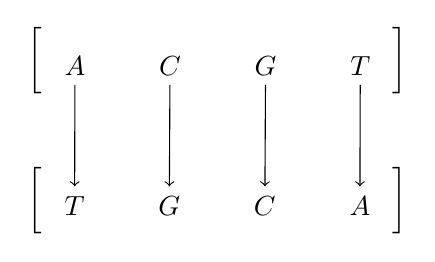
\begin{tikzpicture}[baseline=(current bounding box.center)]
  % Matrix A
  \matrix (A) [matrix of math nodes, left delimiter={[}, right delimiter={]}, row sep=1em, column sep=2em] {
    A & C & G & T \\
  };

  % Matrix B
  \matrix (B) [matrix of math nodes, left delimiter={[}, right delimiter={]}, row sep=1em, column sep=2em, below=3em of A] {
    T & G & C & A \\
  };

  % Draw arrows from A_i to B_i
  \foreach \i in {1,2,3, 4}
    \draw[->] (A-1-\i) -- (B-1-\i);
\end{tikzpicture}
\]

Which is also the consequence of \textbf{\hyperref[THEOCOMPLEMENTS]{Theorem \ref{THEOCOMPLEMENTS}}}. Thus, for the sequence in \textbf{\hyperref[SEQATC]{Equation \ref{SEQATC}}}, the corresponding complement DNA sequence is:

\begin{equation}
\label{SEQATCCOMP}
\lnot\Theta = \langle T A G C G C A T A \rangle
\end{equation}

This ideal can be further appreciated by noticing that the traditional DNA sequence base symbol set (which we shall denote by $\dot{\psi}_{DNA}$), is actually different from $\psi_{DNA}$, and is defined as:

\begin{equation}
\label{SSDNAT}
\dot{\psi}_{DNA} = \langle A, T, C, G \rangle
\end{equation}

We should come to appreciate this special symbol set, or even justify it --- for logical and mathematical analyses, by acknowledging that it depicts not just a sequence of distinct symbols from $\psi_{DNA}$, but also their natural order based on both order of occurrence in $\psi_{DNA}$ \textbf{and} their equivalent \textbf{symbol complements} in $\lnot\psi_{DNA}$! It is such a terrific discovery/realization. And before we proceed, we note that the $\dot{\psi}_{DNA} \rightarrow \lnot\dot{\psi}_{DNA}$ mapping for pairwise-ordered DNA sequences is as such:


\[
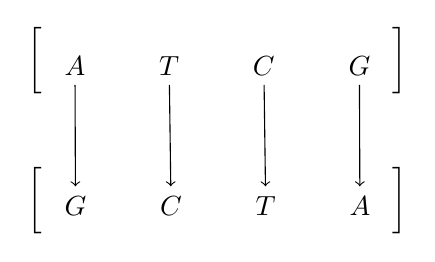
\begin{tikzpicture}[baseline=(current bounding box.center)]
  % Matrix A
  \matrix (A) [matrix of math nodes, left delimiter={[}, right delimiter={]}, row sep=1em, column sep=2em] {
    A & T & C & G \\
  };

  % Matrix B
  \matrix (B) [matrix of math nodes, left delimiter={[}, right delimiter={]}, row sep=1em, column sep=2em, below=3em of A] {
    G & C & T & A \\
  };

  % Draw arrows from A_i to B_i
  \foreach \i in {1,2,3, 4}
    \draw[->] (A-1-\i) -- (B-1-\i);
\end{tikzpicture}
\]


Because, from \textbf{\hyperref[SSDNAT]{Equation \ref{SSDNAT}}}, we can tell that:

\begin{equation}
\label{SSDNATCOMP}
\lnot\dot{\psi}_{DNA} = \langle G, C, T, A \rangle
\end{equation}


Perhaps, and worth checking out, even if momentarily, what would happen when the idea of complement symbols sets and complement sequences is applied to the more commonplace base-10 sequences (aka ``usual numbers")?

First, note that since $\psi_{10}$ --- our choice of symbol for the decimal symbol set, is expressed as such:

\begin{equation}
\label{SSDEC}
\psi_{10}= \langle 0, 1, 2, 3, 4, 5, 6, 7, 8, 9 \rangle
\end{equation}

Then, by \textbf{\hyperref[THEOCOMPLEMENTS]{Theorem \ref{THEOCOMPLEMENTS}}}, its complement is:


\begin{equation}
\label{SSDEC}
\lnot\psi_{10}= \langle 9, 8, 7, 6, 5, 4, 3, 2, 1, 0 \rangle
\end{equation}

So that, for any base-10 digit, the corresponding \textbf{complement digit} is as in the mapping below:


\[
\begin{tikzpicture}[baseline=(current bounding box.center)]
  % Matrix A
  \matrix (A) [matrix of math nodes, left delimiter={[}, right delimiter={]}, row sep=1em, column sep=2em] {
    0 & 1 & 2 & 3 & 4 & 5 & 6 & 7 & 8 & 9\\
  };

  % Matrix B
  \matrix (B) [matrix of math nodes, left delimiter={[}, right delimiter={]}, row sep=1em, column sep=2em, below=3em of A] {
    9 & 8 & 7 & 6 & 5 & 4 & 3 & 2 & 1 & 0\\
  };

  % Draw arrows from A_i to B_i
  \foreach \i in {1,2,3,4,5,6,7,8,9,10}
    \draw[->] (A-1-\i) -- (B-1-\i);
\end{tikzpicture}
\]

Such a peculiar cipher! Because, usual/familiar number sequences such as the \textbf{Hi-Fi o-SSI}\cite{adtpaper}, defined as such:

\begin{equation}
\Theta_{HiFi} = 8 6 4 9 1 3 7 5 2 0
\end{equation}

Has the complement:


\begin{equation}
\lnot\Theta_{HiFi} = 1 3 5 0 8 6 2 4 7 9
\end{equation}

Which, given how that special sequence was derived/discovered(see \textbf{Section 5.1} in \cite{ossipaper} or \textbf{Equation 19} in the same paper), it is interesting to note that its complement under $\psi_{10}$ is also an \textit{orthogonal symbol set identity}! For those who have studied the o-SSI paper\cite{ossipaper}, this can really be exciting for the study of symbol sets and sequences in general --- yes, even for nucleic acid sequences! But, that said, of course, it shouldn't come as a surprise, since, in simple terms, a sequence's complement is just one very special kind anagram among the set of all potential anagrams it can have, and so, before we leave the base-10 case, we can note that if some sequence $\Theta_{10}: \mathbb{N} \times \psi_{10}$ is a base-10 o-SSI, then its complement is also a base-10 o-SSI, and in fact, in general --- even for non-numeric symbol sets such as $\psi_{na}, \psi_{DNA}$ or special $\psi_{RNA}$, that:\\


\begin{theo}[\textbf{Complement of an o-SSI is an o-SSI}]
\label{THEOCOMPLOSSI}
If some sequence $\Theta: \mathbb{N} \times \psi_\beta$ is an orthogonal symbol set identity for the base $\beta$, then its complement, $\lnot\Theta$ is also an orthogonal symbol set identity for $\beta$.\\
\end{theo}

We shall see how \textbf{\hyperref[THEOCOMPLOSSI]{Theorem  \ref{THEOCOMPLOSSI}}} might be applied, when dealing with algorithmic anagrammatization of sequences such as $\psi_{10}$ in \textbf{\hyperref[SECRSG]{Chapter \ref{SECRSG}}}.

\section{Potential Applications of Sequence Complements or Inverses}
\label{SECAPPCOMPLEMENTS}

First, in genetics and analysis of genetic code sequences, note that for especially na-Sequences in say the \textit{non-native}(non-storage) form, such as the processed/derivative RNA-sequences, it might sometimes be useful to determine if some two sequences are the same, equivalent or closely related, even though their apparent ordering of members, or even member composition looks unlike, \textbf{as long as their cardinalities are the same}\footnote{This requirement to have their sizes the same, is a natural consequence of how a sequence and its anagrams relate --- see \cite{adtpaper}}.

We should note, and interestingly so, that the complement of any sequence $\Theta$, which is $\lnot\Theta$, is just an anagram of $\Theta$, and that in general, we can comfortably say:


\begin{theo}[\textbf{Equivalence of Sequences under the Complement Transform}]
\label{THEOCOMPEQUIV}
If two sequences $\Theta$ and $\Omega$ that are \textbf{not equal}, but which do have the same cardinality and similar distribution of members, then they are essentially equivalent under the sequence complement transform.

\begin{proof}
The proofs are several:
\begin{enumerate}
\item Since $\invpi(\Theta) = \invpi(\Omega)$ and $\forall \alpha \in \Theta \quad \exists \rho \in \Omega: \alpha = \rho$ or equivalently, that $\forall a_i \in \Theta, \invpi(a_i \in \Theta) = \invpi(a_i \in \Omega)$, then there exists some anagram of $\Theta$, denoted $\Theta^*$ such that $\Theta^* \xrightarrow{O_{complement}(\cdot)} \Omega$, which is possible by \textbf{\hyperref[THEOCOMPLEMENTS]{Theorem \ref{THEOCOMPLEMENTS}}}.
\item Because sequence complements are anagrams of each other, then if the two sequences are complements of each other, we expect that by the definition of the complement transformer (see \textbf{\hyperref[TRANSCOMPL]{Transformer \ref{TRANSCOMPL}}}), $\Omega = \lnot\Theta$ or that $\Theta = \lnot\Omega$.
\item We might also proceed by use of \textbf{modal sequences} (see \textbf{Definition 1} in \cite{transformatics}): Given the conditions on the two sequences, we then expect that if $\Theta$ is a sequence complement of $\Omega$ or vice-versa, then, computing their corresponding modal sequence statistic should result in the following result: $\overset{>}{\Theta} = \lnot(\overset{>}{\lnot\Omega})$ or equivalently, $\overset{>}{\Omega} = \lnot(\overset{>}{\lnot\Theta})$
\end{enumerate}
\end{proof}

\end{theo}


Note that, for RNA, since $\psi_{RNA} = \langle A, C, G, U \rangle$ (\textbf{\hyperref[EQRNASS]{Equation \ref{EQRNASS}}}), then: 

\begin{equation}
\label{EQRNACOMP}
\lnot\psi_{RNA} = \langle U, G, C, A \rangle
\end{equation}

And this is what we'd expect via the complement mapping:


\[
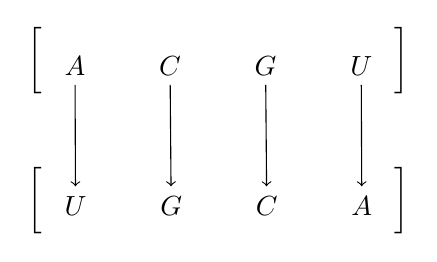
\begin{tikzpicture}[baseline=(current bounding box.center)]
  % Matrix A
  \matrix (A) [matrix of math nodes, left delimiter={[}, right delimiter={]}, row sep=1em, column sep=2em] {
    A & C & G & U \\
  };

  % Matrix B
  \matrix (B) [matrix of math nodes, left delimiter={[}, right delimiter={]}, row sep=1em, column sep=2em, below=3em of A] {
    U & G & C & A \\
  };

  % Draw arrows from A_i to B_i
  \foreach \i in {1,2,3, 4}
    \draw[->] (A-1-\i) -- (B-1-\i);
\end{tikzpicture}
\]


But, since the traditional pairwise ordered symbol set for RNA, $\dot{\psi}_{RNA}$ is


\begin{equation}
\label{EQRNATRAD}
\dot{\psi}_{RNA} = \langle A, U, C, G \rangle
\end{equation}

Then its corresponding complement,$\lnot\dot{\psi}_{RNA}$, is

\begin{equation}
\label{EQRNATRADCOMP}
\lnot\dot{\psi}_{RNA} = \langle G, C, U, A \rangle
\end{equation}

And so we have the associated complement mapping as

\[
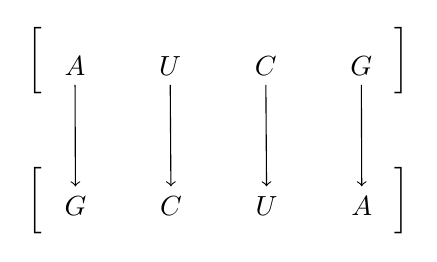
\begin{tikzpicture}[baseline=(current bounding box.center)]
  % Matrix A
  \matrix (A) [matrix of math nodes, left delimiter={[}, right delimiter={]}, row sep=1em, column sep=2em] {
    A & U & C & G \\
  };

  % Matrix B
  \matrix (B) [matrix of math nodes, left delimiter={[}, right delimiter={]}, row sep=1em, column sep=2em, below=3em of A] {
    G & C & U & A \\
  };

  % Draw arrows from A_i to B_i
  \foreach \i in {1,2,3, 4}
    \draw[->] (A-1-\i) -- (B-1-\i);
\end{tikzpicture}
\]


So, that, for some RNA-sequence such as $\Theta_{met}$:


\begin{equation}
\Theta_{met} = \langle A, U, G \rangle
\end{equation}


Which is the famous START-codon \textbf{Methionine} (see \textbf{\hyperref[TAB2]{Table \ref{TAB2}}}), has as its corresponding nucleic acid sequence complement under $\dot{\psi}_{RNA}$:

\begin{trans}
\label{TRANSGCA}
$\Theta_{met} \xrightarrow{O_{complement}(\Theta,\dot{\psi}_{RNA})}  \langle G, C, A \rangle$\\
That codon isn't the same as the source (ATG/AUG/Methionine), but there's some debate concerning what it actually is called --- \textbf{Table 1} in \cite{gregory1987oxford} names codon GCA as \textbf{Arginine}, while Wikipedia\cite{wikipedia_codon_tables} names it \textbf{Alanine}.
\end{trans}

While --- \textbf{and important to note}, its complement under $\psi_{RNA}$ is [indeed] different!

\begin{trans}
\label{TRANSUAC}
$\Theta_{met} \xrightarrow{O_{complement}(\Theta,\psi_{RNA})}  \langle U, A, C \rangle$
\\
and we know that codon UAC is Tyrosine\cite{wikipedia_codon_tables}\footnote{Concerning this particular codon, TAC/UAC, we find that though the Wikipedia reference tables assign it the name Tyrosine in both the DNA and RNA encodings, and yet, the physical reference we have at hand\cite{gregory1987oxford} (perhaps now out-of-date), assigns the name ``Methionine" to TAC --- Table 1 in that reference book did not list RNA codes, but we still would expect to use TAC to look-up the correct name for UAC.}.
\end{trans}

It should perhaps be immediately noticeable that the ability to derive new/different/special sequences such as complement codons from ordinary na-Sequences might have some useful if not exciting applications as well as problems it awakens for the geneticists, molecular biologists and researchers of gene-sequencing\footnote{For those that do not know: Gene sequencing is the process of determining the exact order of nucleotides --- A, T, C and G --- in a segment of DNA that makes up a gene. It is like reading the biological ``code" that instructs cells how to build proteins and regulate functions\cite{copilot_dna_assistant}.} and analysis. For example, apart from acknowledging that na-Sequence's complements denote potentially legitimate na-helix strand partners for any two sequences (in the form $\Theta$ and $\lnot\Theta$), it would be further rewarding, to determine what other important things we might learn about how important sequences such as na-Sequences, especially relative to how they are utilized in nature, behave or alter their usual function, if replaced by their complements either partially or wholly. Definitely, even for any ordered sequences in general... it must be exhilirating to discover what other things we can learn with or from them, via these kinds of sequence transforms. 

It is already interesting to note that under complement transforms (which are special kinds of anagrams), the natural/universal protein synthesis START-codon AUG/ATG is equivalent to GCA (\textbf{\hyperref[TRANSGCA]{Transformation \ref{TRANSGCA}}}) or UAC (\textbf{\hyperref[TRANSUAC]{Transformation \ref{TRANSUAC}}}), but, \textbf{are those other codons also START-codons?} That said, is there a possibility that some natural process or genetic code translation or transformation might naturally produce ATG or AUG from any of those corresponding [symbolic] complement sequences? What would this teach us about natural/biological processors? What of the possibilities of using synthetic/artificial processors to render such complement operations useful? And is it actually possible to \textit{transmute} one set of nucleic acid sequences into another, with entirely different functions and identity via leveraging na-complements or complement transforms?




\chapter{Sequence Analysis Using The Anagram Distance and the Modal Sequence Statistic}
\label{SEC4A}

\hl{--- FINISHED PROOF-READING UP TO HERE}

We are going to talk about the matter of comparing or analyzing two or more na-Sequences using especially statistical measures that have been set down by transformatics theory for especially ordered sequences. 

\section{Six Sequences and Four Scenarios}
\label{SEC4ASEQ}

In particular, we shall be looking at na-Sequence analysis through lens of measures we have formalized earlier on, and shall break down our analysis into four representative scenarios:

\begin{enumerate}
\item \textbf{Scenario A:} Given some two particular instances of na-Sequences, $\Theta1_n$ and $\Theta2_n$, of the same length, $n$, and with similar symbol sets ($\psi_{na}(\Theta1_n) = \psi_{na}(\Theta2_n)$), \textbf{how to quantify how similar or dissimilar} they are?
\item \textbf{Scenario B:} Given some two particular instances of na-Sequences, $\Theta1_n$ and $\Theta2_k$, of different lengths, $n$ and $k$, but with similar symbol sets ($\psi_{na}(\Theta1_n) = \psi_{na}(\Theta2_k)$), how to quantify how similar or dissimilar they are?
\item \textbf{Scenario C:} Given some two particular instances of na-Sequences, $\Theta1_n$ and $\Theta2_k$, of \textbf{different lengths}, $n$ and $k$ and with different symbol sets ($\psi_{na}(\Theta1_n) \neq \psi_{na}(\Theta2_k)$), how to quantify how similar or dissimilar they are?
\item \textbf{Scenario D:} Finally, how, when given a particular na-Sequence, $Q_k$, and two collections/samples of other sequences ($\Theta1, \Theta2, \Theta3,..., \Theta m$) and ($\Omega1, \Omega2, \Omega3,..., \Omega n$) of potentially dissimilar lengths, and that belong to \textbf{labeled or classified populations} --- POPA and POPB, to determine which of the two populations the query sequence, $Q_k$, best-belongs to (so we classify it under one of those labels), as well as determine which of the \textbf{particular} sample member sequences from either collections it is closest to?
\end{enumerate}

Note that in conducting these analyses, we shall especially exploit the sequence-specific measures, $\tilde{A}(\cdot)$, the Anagram Distance Measure\cite{adtpaper}\cite{transformatics}, and $\overset{>}{\Theta}$, the Modal Sequence Statistic\cite{transformatics}, and that we shall use the following representative, even though somewhat hypothetical (for the first four), na-Sequences:

\begin{equation}
{\Theta1}_{DNA} = \langle TAC GGG CAT TCC \rangle\\
\end{equation}

\begin{equation}
{\Theta2}_{RNA} = \langle AUG AUG CGC GGG CAT AUC \rangle\\
\end{equation}

\begin{equation}
{\Theta3}_{DNA} = \langle ATA ATGG GGG CAT TGA \rangle\\
\end{equation}

\begin{equation}
{\Theta4}_{DNA} = \langle TAC TCC GGG CAT\rangle\\
\end{equation}

\begin{multline}
\Theta_{insulin} =  \texttt{ATGGCCCTGTGGATGCGCCTCCTGCCCCTGCTGGCGCTGCTGGCCCTCTGGGGACC}\\
\texttt{CCAGCCGCAGCCTTTGTGAACCAACACCTGTGCGGCTCACACCTGGTGGAAGCTCTCTAC}\\
\texttt{CTAGTGTGCGGGGAACGAGGCTTCTTCTACACACCCAAGACCCGCCGGGAGGCAGAGGAC}\\
\texttt{CTGCAGGTGGGGCAGGTGGAGCTGGGCGGGGGCCCTGGTGCAGGCAGCCTGCAGCCCTTG}\\
\texttt{GCCCTGGAGGGGTCCCTGCAGAAGCGTGGCATTGTGGAACAATGCTGTACCAGCATCTGC}\\
\texttt{TCCCTCTACCAGCTGGAGAACTACTGCAACTAG}
\end{multline}

\small
\begin{multline}
\Theta_{rbcl} = 
AUGAAUUGCUUUGGAGGAGUUGCUUUGGCUUUGGAGGAGUUUGCUUUGGCUUUGGAGGAG\\
UUUGCUUUGGCUUUGGAGGAGUUUGCUUUGGCUUUGGAGGAGUUUGCUUUGGCUUUGGAG\\
GAGUUUGCUUUGGCUUUGGAGGAGUUUGCUUUGGCUUUGGAGGAGUUUGCUUUGGCUUUG\\
GAGGAGUUUGCUUUGGCUUUGGAGGAGUUUGCUUUGGCUUUGGAGGAGUUUGCUUUGGCU\\
UUGGAGGAGUUUGCUUUGGCUUUGGAGGAGUUUGCUUUGGCUUUGGAGGAGUUUGCUUUG\\
GCUUUGGAGGAGUUUGCUUUGGCUUUGGAGGAGUUUGCUUUGGCUUUGGAGGAGUUUGCU\\
UUGGCUUUGGAGGAGUUUGCUUUGGCUUUGGAGGAGUUUGCUUUGGCUUUGGAGGAGUUU\\
GCUUUGGCUUUGGAGGAGUUUGCUUUGGCUUUGGAGGAGUUUGCUUUGGCUUUGGAGGAG\\
UUUGCUUUGGCUUUGGAGGAGUUUGCUUUGGCUUUGGAGGAGUUUGCUUUGGCUUUGGAG\\
GAGUUUGCUUUGGCUUUGGAGGAGUUUGCUUUGGCUUUGGAGGAGUUUGCUUUGGCUUUG\\
GAGGAGUUUGCUUUGGCUUUGGAGGAGUUUGCUUUGGCUUUGGAGGAGUUUGCUUUGGCU\\
UUGGAGGAGUUUGCUUUGGCUUUGGAGGAGUUUGCUUUGGCUUUGGAGGAGUUUGCUUUG\\
GCUUUGGAGGAGUUUGCUUUGGCUUUGGAGGAGUUUGCUUUGGCUUUGGAGGAGUUUGCU\\
UUGGCUUUGGAGGAGUUUGCUUUGGCUUUGGAGGAGUUUGCUUUGGCUUUGGAGGAGUUU\\
GCUUUGGCUUUGGAGGAGUUUGCUUUGGCUUUGGAGGAGUUUGCUUUGGCUUUGGAGGAG\\
UUUGCUUUGGCUUUGGAGGAGUUUGCUUUGGCUUUGGAGGAGUUUGCUUUGGCUUUGGAG\\
GAGUUUGCUUUGGCUUUGGAGGAGUUUGCUUUGGCUUUGGAGGAGUUUGCUUUGGCUUUG\\
GAGGAGUUUGCUUUGGCUUUGGAGGAGUUUGCUUUGGCUUUGGAGGAGUUUGCUUUGGCU\\
UUGGAGGAGUUUGCUUUGGCUUUGGAGGAGUUUGCUUUGGCUUUGGAGGAGUUUGCUUUG\\
GCUUUGGAGGAGUUUGCUUUGGCUUUGGAGGAGUUUGCUUUGGCUUUGGAGGAGUUUGCU\\
UUGGCUUUGGAGGAGUUUGCUUUGGCUUUGGAGGAGUUUGCUUUGGCUUUGGAGGAGUUU\\
GCUUUGGCUUUGGAGGAGUUUGCUUUGGCUUUGGAGGAGUUUGCUUUGGCUUUGGAGGAG\\
UUUGCUUUGGCUUUGGAGGAGUUUGCUUUGGCUUUGGAGGAGUUUGCUUUGGCUUUGGAG\\
GAGUUUGCUUUGGCUUUGGAGGAGUUUGCUUUGGCUUUGGAGGAGUUUGCUUUGGCUUUG\\
GAGGAGUUUGCUUUGGCUUUGGAGGAGUUUGCUUUGGCUUUGGAGGAGUUUGCUUUGGCU\\
UUGGAGGAGUUUGCUUUGGCUUUGGAGGAGUUUGCUUUGGCUUUGGAGGAGUUUGCUUUG\\
GCUUUGGAGGAGUUUGCUUUGGCUUUGGAGGAGUUUGCUUUGGCUUUGGAGGAGUUUGCU\\
UUGGCUUUGGAGGAGUUUGCUUUGGCUUUGGAGGAGUUUGCUUUGGCUUUGGAGGAGUUU\\
GCUUUGGCUUUGGAGGAGUUUGCUUUGGCUUUGGAGGAGUUUGCUUUGGCUUUGGAGGAG\\
UUUGCUUUGGCUUUGGAGGAGUUUGCUUUGGCUUUGGAGGAGUUUGCUUUGGCUUUGGAG\\
GAGUUUGCUUUGGCUUUGGAGGAGUUUGCUUUGGCUUUGGAGGAGUUUGCUUUGGCUUUG\\
GAGGAGUUUGCUUUGGCUUUGGAGGAGUUUGCUUUGGCUUUGGAGGAGUUUGCUUUGGCU\\
UUGGAGGAGUUUGCUUUGGCUUUGGAGGAGUUUGCUUUGGCUUUGGAGGAGUUUGCUUUG\\
GCUUUGGAGGAGUUUGCUUUGGCUUUGGAGGAGUUUGCUUUGGCUUUGGAGGAGUUUGCU\\
UUGGCUUUGGAGGAGUUUGCUUUGGCUUUGGAGGAGUUUGCUUUGGCUUUGGAGGAGUUU\\
GCUUUGGCUUUGGAGGAGUUUGCUUUGGCUUUGGAGGAGUUUGCUUUGGCUUUGGAGGAG\\
UUUGCUUUGGCUUUGGAGGAGUUUGCUUUGGCUUUGGAGGAGUUUGCUUUGGCUUUGGAG\\
GAGUUUGCUUUGGCUUUGGAGGAGUUUGCUUUGGCUUUGGAGGAGUUUGCUUUGGCUUUG\\
GAGGAGUUUGCUUUGGCUUUGGAGGAGUUUGCUUUGGCUUUGGAGGAGUUUGCUUUGGCU\\
UUGGAGGAGUUUGCUUUGGCUUUGGAGGAGUUUGCUUUGGCUUUGGAGGAGUUUGCUUUG\\
GCUUUGGAGGAGUUUGCUUUGGCUUUGGAGGAGUUUGCUUUGGCUUUGGAGGAGUUUGCU\\
UUGGCUUUGGAGGAGUUUGCUUUGGCUUUGGAGGAGUUUGCUUUGGCUUUGGAGGAGUUU\\
GCUUUGGCUUUGGAGGAGUUUGCUUUGGCUUUGGAGGAGUUUGCUUUGGCUUUGGAGGAG\\
UUUGCUUUGGCUUUGGAGGAGUUUGCUUUGGCUUUGGAGGAGUUUGCUUUGGCUUUGGAG\\
GAGUUUGCUUUGGCUUUGGAGGAGUUUGCUUUGGCUUUGGAGGAGUUUGCUUUGGCUUUG\\
GAGGAGUUUGCUUUGGCUUUGGAGGAGUUUGCUUUGGCUUUGGAGGAGUUUGCUUUGGCU\\
UUGGAGGAGUUUGCUUUGGCUUUGGAGGAGUUUGCUUUGGCUUUGGAGGAGUUUGCUUUG\\
GCUUUGGAGGAGUUUGCUUUGGCUUUGGAGGAGUUUGCUUUGGCUUUGGAGGAGUUUGCU\\
UUGGCUUUGGAGGAGUUUGCUUUGGCUUUGGAGGAGUUUGCUUUGGCUUUGGAGGAGUUU\\
GCUUUGGCUUUGGAGGAGUUUGCUUUGGCUUUGGAGGAGUUUGCUUUGGCUUUGGAGGAG\\
UUUGCUUUGGCUUUGGAGGAGUUUGCUUUGGCUUUGGAGGAGUUUGCUUUGGCUUUGGAG\\
GAGUUUGCUUUGGCUUUGGAGGAGUUUGCUUUGGCUUUGGAGGAGUUUGCUUUGGCUUUG\\
GAGGAGUUUGCUUUGGCUUUGGAGGAGUUUGCUUUGGCUUUGGAGGAG
\end{multline}
\Large


%The first four sequences are merely hypothetical, and intentionally small/short, with $\Theta1_{DNA}$, $\Theta3_{DNA}$ and $\Theta4_{DNA}$ being DNA-sequences, while $\Theta2_{RNA}$ is just some RNA-sequence. $\Theta_{insulin}$ is a DNA-sequence we have already encountered in \textbf{\hyperref[SEC2]{Chapter \ref{SEC2}}} (see \textbf{\hyperref[EQINSULIN]{Equation \ref{EQINSULIN}}}), while the most verbose sequence we shall encountered in this work is named $\Theta_{rbcl}$ and is a real-life, biologically relevant RNA-sequence from a well-known plant protein: \textbf{RbcL}\footnote{$\Theta_{rbcl}$ is actually just a sample mRNA Sequence (partial, from \textit{Arabidopsis thaliana} RbcL gene), and is excerpted from a paper that includes the \textit{Arabidopsis thaliana} chloroplast genome, which contains the rbcL gene encoding the large subunit of RuBisCO\cite{Sato1999ArabidopsisChloroplastGenome}.}, the large subunit of \textbf{RuBisCO} --- the enzyme responsible for carbon fixation in photosynthesis. It is one of the most abundant and essential proteins in plants\cite{copilot_dna_assistant}.

\section{A First Analysis}
\label{SECFANAL}

Before we dive into the matter of solving the analytic problems under the four scenarios introduced in \textbf{\hyperref[SEC4ASEQ]{Section \ref{SEC4ASEQ}}} above, we shall want to begin with a background analysis that shall give us some high-level insights about any of the sequences in our problem set. In particular, we are going to start by analyzing each of those sequences, so as to know the following basic facts:

\begin{enumerate}
\item What is the sequence's symbol set: $\psi(\Theta) = ?$
\item Which of the three nucleic acid symbol sets does the sequence belong to --- $\psi_{DNA}$, $\psi_{RNA}$ or $\psi_{na}$
\item What is the relative frequency of each sequence's symbol-set members? $\forall \rho \in \psi(\Theta), \invpi(\rho \in \Theta) = ?$
\item How long is the sequence as a flat-structure sequence: $\invpi(\Theta) = ?$
\item How many codons does the sequence contain? $\Theta \rightarrow \Theta^*: \mathbb{N} \times \psi_{na}^3, \invpi(\Theta^*) = ?$
\end{enumerate}

For purposes of helping others replicate the analyses and results we shall obtain, we recommend that the following analysis method be used: We can use the TEA\footnote{Instructions for how to install and use TEA/Transforming Executable Alphabet general-purpose text-processing oriented computer programming language are offered via the project's GitHub: \url{https://github.com/mcnemesis/cli_tttt}}\cite{Lutalo2024_taz}\cite{cli_tttt} text-processing programming language --- by the author, via its \texttt{tttt} Linux/Unix package to compute some of the analyses we wish to do via the command-line.

\begin{enumerate}
\item {\textbf{To Process Sequence on Command-Line?} For example, copy-and-paste sequence $\Theta1$ into a file named \texttt{theta1\_dna.txt}}
\item {\textbf{To compute the sequence symbol set?} For example, for $\Theta1$, run the following command against the sequence file to display the unique symbols in the sequence, in their natural order of first-occurrence within the sequence:

\begin{verbatim}
cat theta1_dna.txt | tttt -c "b:"
TACG
\end{verbatim}

}
\item {\textbf{To compute the modal sequence statistic?} First, note that the \textbf{modal sequence statistic} is well introduced, defined and how to use it demonstrated in \cite{transformatics}\footnote{See \textbf{Definition 1} in \cite{transformatics}}. That said, for example, for $\Theta1$, run the following command against the sequence file to display the unique symbols in the sequence, in their order of most frequent first, and/or their natural order of first-occurrence within the sequence:

\begin{verbatim}
cat theta1_dna.txt | tttt -c "u!"":"
CGTA
\end{verbatim}
Note that the actual command/TEA-code for this is just ``u!:", however, because of the way the Linux command-line treats the `!' symbol as a special character --- even inside strings, we must cleverly use it in a manner such as shown; we write ``u!"``:" to avoid the \textit{``unrecognized history modifier"} error if that code is written directly on the terminal. This shall apply to all the other cases where we must deal with the TEA command qualifier `!"\cite{Lutalo2024_taz} The other workaround is to \textbf{first turn off the BASH history expansion modifier}, this, so that we can just write clean TEA code such as ``u!:" without errors. So, to disable history expasion for the \textit{active/current session} in your terminal, just run the command:

\begin{verbatim}
set +H
\end{verbatim}

And after that, you can just write clean TEA code for the above task as such:
\begin{verbatim}
cat theta1_dna.txt | tttt -c u!:
CGTA
\end{verbatim}
}
\item {\textbf{To compute the distribution of symbols within a sequence?} For example, to compute how many times the symbol `T' occurs in $\Theta1$, we can merely run the code:

\begin{verbatim}
cat theta1_dna.txt | tttt -c "d!:T|g:|v:|v!:"
3
\end{verbatim}
And for the symbol `C', we just modify that code to count for `C' as such:


\begin{verbatim}
cat theta1_dna.txt | tttt -c "d!:C|g:|v:|v!:"
4
\end{verbatim}

But if we wish to do the same for all distinct symbols within the sequence $\Theta1$ --- \textbf{and especially without having to explicitly list which symbols we are counting within the TEA code}, we could have used ``u!:" as in the previous task, since that TEA command counts how many times each unique symbol occurs in a sequence so as to compute the modal sequence, however, currently (with TEA version \textbf{1.0.8}\cite{cli_tttt}), the actual frequencies aren't returned with the output of ``u!:", and so, we shall want to use a work-around leveraging the above method for computing the frequency of each symbol in the input sequence. We can use the following non-trivial TEA program for that then:

\begin{verbatim}
 cat theta1_dna.txt | tttt -c "v:vSEQ|v:vANA:{}|u!:|v:vMS|l:lMS|y:vMS|d!:^.|v:vSY|y:vMS|d:^.|v:vMS|y:vSEQ|d*!:vSY|g:|v:|v!:|v:vSYN|g*:{}:vSY:vSYN|x*:vANA|v:vANA|y:vMS|f:^$:lFIN|j:lMS|l:lFIN|y:vANA"
C4G3T3A2
\end{verbatim}

The essential result from running that program against $\Theta1$ is the string \textbf{C4G3T3A2}, which tells us that `C' occurs 4 times, `G' 3 times, ... , and then `A' only 2 times. 
}
\item {\textbf{To compute the cardinality of a sequence?} For example, for $\Theta2$, run the following command against the sequence file to display the total number of all symbols within the sequence:

\begin{verbatim}
cat theta2_rna.txt | tttt -c "v:|v!:"
18
\end{verbatim}

To confirm if TEA is telling us the correct thing, we can also count the characters in that sequence (assuming we pasted just the sequence symbols into the file and nothing else, and no delimiters between them), using the standard Linux/Unix command ``wc'' as such:

\begin{verbatim}
cat theta2_rna.txt | wc -c
18
\end{verbatim}

}
\end{enumerate}


Such is the power of the sequence analysis we can do with the TEA language, without any sophisticated tools. Thus, shall we analyze all the other sequences in our problem set, and to simplify things, we shall merely tabulate the analysis results for all six sequences as such:


\begin{table}[H]
  \Large
	\begin{tabular}[t]{|p{1.5cm}||p{3cm}|p{2cm}|p{6cm}|p{1.5cm}|p{1.5cm}|}
	\hline
	na-Seq & Unspecific Sequence Symbol Set: $\psi(\Theta)$ & Closest Parent Symbol Set & \makecell{Modal Sequence\\Statistic, $\overset{>}{\Theta}$\\ and Symbol\\ Distribution:\\ $\invpi(\rho \in \Theta)$} & $\invpi(\Theta)$ &  \makecell{Codon\\ Count:\\ $\invpi(\Theta^*)$\\ $\approx \frac{\invpi(\Theta)}{3}$}\\
	\hline
	\hline
	
	%first sequence...
	${\Theta1}_{DNA}$ & $\langle T, A, C, G \rangle$ & $\psi_{DNA}$ &  
	\centering
	\begin{tabular}[t]{|c|c|c|c|}
		C & G & T & A\\
		\hline
		4 & 3 & 3 & 2\\	
		\hline
	 \end{tabular} & 12 & 4\\
		\hline	 
	\hline
	
	%second sequence...
	${\Theta2}_{RNA}$ & $\langle A, U, G, C, T \rangle$ & $\psi_{na}$ &  
	\centering
	\begin{tabular}[t]{|c|c|c|c|c|}
		G & C & A & U & T\\
		\hline
		6 & 4 & 4 & 3 & 1\\	
		\hline
	 \end{tabular} & 18 & 6\\
	 
		\hline	 
	\hline

%third sequence...
	${\Theta3}_{DNA}$ & $\langle A, T, G, C \rangle$ & $\psi_{DNA}$ &  
	\centering
	\begin{tabular}[t]{|c|c|c|c|}
		G & A & T & C\\
		\hline
		6 & 5 & 4 & 1\\	
		\hline
	 \end{tabular} & 16 & $5.3\bar{3}$\\
	\hline	 
	\hline
	
	
	%fourth sequence...
	${\Theta4}_{DNA}$ & $\langle T, A, C, G \rangle$ & $\psi_{DNA}$ &  
	\centering
	\begin{tabular}[t]{|c|c|c|c|}
		C & G & T & A\\
		\hline
		4 & 3 & 3 & 2\\	
		\hline
	 \end{tabular} & 12 & 4\\
	\hline	 
	\hline
	
	
	%fourth sequence...
	${\Theta}_{insulin}$ & $\langle A, T, G, C \rangle$ & $\psi_{DNA}$ &  
	\centering
	\begin{tabular}[t]{|c|c|c|c|}
		G & C & T & A\\
		\hline
		108 & 105 & 60 & 56\\	
		\hline
	 \end{tabular} & 329 & $109.6\bar{6}$\\
	\hline	 
	\hline
	
	%fifth sequence...
	${\Theta}_{rbcl}$ & $\langle A, U, G, C \rangle$ & $\psi_{RNA}$ &  
	\centering
	\begin{tabular}[t]{|c|c|c|c|}
		U & G & A & C\\
		\hline
		1355 & 1207 & 305 & 301\\	
		\hline
	 \end{tabular} & 3168 & 1056\\
	\hline	 
	\hline	
	
	              
\end{tabular}
 \caption{A First Analysis of the 5 na-Sequences from \textbf{\hyperref[SEC4ASEQ]{Section \ref{SEC4ASEQ}}}}
  \label{TABFAN}
\end{table}





\section{SCENARIO A --- the anagram distance measure}
\label{SECSCENA}

\begin{quote}
\small
\texttt{
Given some two particular instances of na-Sequences, $\Theta1_n$ and $\Theta2_n$, of the same length, $n$, and with similar symbol sets ($\psi_{na}(\Theta1_n) = \psi_{na}(\Theta2_n)$), how to quantify how similar or dissimilar they are?}
\end{quote}

So, in this scenario, we are basically given some two particular na-Sequences, of the same length, and which have similar symbol sets, and are tasked with how to quantify their similarity or dissimilarity.

Looking at our example sequences above in \textbf{\hyperref[TABFAN]{Table \ref{TABFAN}}}, only two sequences satisfy the necessary conditions --- $\Theta1$ and $\Theta4$, which both have length \textbf{12} and which have similar symbol sets under base-na\footnote{Formally defined in \textbf{\hyperref[DEFUNA]{Definition \ref{DEFUNA}}}} --- $\psi_{na}(\Theta1) = \psi_{na}(\Theta4) = \langle A, C, G, T \rangle$, but also their unspecific sequence symbol sets are already similar.

Actually, this case is very telling concerning what might actually happen with na-Sequences --- essentially, we note that, despite the two sequences \textbf{actually being different} --- for example, $\Theta1$ ends with codon \texttt{TTC}, while $\Theta4$ ends with \texttt{CAT}, and yet, looking at their breakdown analysis via \textbf{\hyperref[TABFAN]{Table \ref{TABFAN}}}, we see that \textbf{they almost seem to be the same!} They have the same sequence symbol set, the same parent symbol set, the same modal sequence and symbol distribution, the same sequence length and thus same number of codons! So, how exactly can we quantifiably distinguish between such sequences in real life?

At this juncture, it definitely might make sense to recall what the purpose of the \textbf{Anagram Distance Measure}\cite{adtpaper} --- it essentially is a measure that allows us to tell if any two sequences that might contain the same exact distinct symbols, but possibly in different proportions and/or order, are different or not. So, since we can't use the usually sufficient \textbf{modal sequence statistic}\cite{transformatics} to distinguish between these two actually different sequences, let us attempt to compute their anagram distance instead\footnote{It shall be \textbf{very important} to bring to mind here, the fact that, the cases where comparing sequences or datasets using the ADM might not seem obvious, but as we already saw in a detailed attempt to distinguish between actually different sequences using many various traditional statistical measures  (of variation moreover) that all failed to show a difference between some two test sequences --- see \textbf{Table 1} in \cite{transformatics}, one shouldn't take ADM any less serious even for non-numerical data such as analysis nucleic acid sequences!}. 

\begin{center}
\fbox{\begin{minipage}{0.9\textwidth}
\large
\textbf{NOTE:}\\
 A Quick Recap \textbf{Concerning Interpreting ADM, $\tilde{A}(\Theta,\Theta^*)$} \\

The Anagram Distance Measure (ADM), associated testing method, background and justifications for the new statistic were first laid out in the seminal paper\cite{adtpaper} introducing that measure and its theory. That work was later advanced in the transformatics paper\cite{transformatics}, and essentially, we can note that:

\begin{itemize}
\item{Given any two sequences, $\Theta$ and $\Theta^*$, that ideally should be of the same length, and with the same sequence symbol set, then we compute the anagram distance between them via the formula:

\begin{equation}
\label{EQADM}
\tilde{A}(\Theta \rightarrow \Theta^*) = \frac{1}{\invpi(\Theta)} \times \sum\limits_{i=1}^{\invpi(\Theta)} |I(\omega_i,\Theta^*) - i|
\end{equation}
}
\item {
And that we can interpret the results --- which shall always be a positive real number ($\mathbb{R^+}$) as such:

\begin{equation}
\label{EQINTADM}
\tilde{A}(\Theta \rightarrow \Theta^*) = \begin{cases}
0, & \Theta = \Theta^*,  \text{no differences}\\
< 1, & \Theta \approx \Theta^*, \text{different in at minimum two positions}\\
= 1, & \Theta \neq \Theta^*, \text{all members shifted by exactly 1 position}\\
> 1, & \Theta \ll \Theta^*, \text{potential indication there is chaos.}
\end{cases}
\end{equation}

For a quick primer, on how this works out, assume we have $\Theta_1=\langle a, b, c\rangle$, $\Theta_2=\langle a, c, b\rangle$, $\Theta_3=\langle b, c, a\rangle$, $\Theta_4=\langle c, a, b\rangle$, $\Theta_5=\langle b, a, c\rangle$. Then we can see that:

\begin{enumerate}
\item $\tilde{A}(\Theta_1,\Theta_2) = \frac{1}{3}(|1-1|+|2-3|+|3-2|) = \frac{2}{3} < 1$
\item $\tilde{A}(\Theta_1,\Theta_3) = \frac{1}{3}(|1-3|+|2-1|+|3-2|) = \frac{4}{3} > 1$
\item $\tilde{A}(\Theta_1,\Theta_4) = \frac{1}{3}(|1-2|+|2-3|+|3-1|) = \frac{4}{3} > 1$
\item $\tilde{A}(\Theta_1,\Theta_1) = \frac{1}{3}(|1-1|+|2-2|+|3-3|) = \frac{0}{3} = 0$
\item $\tilde{A}(\Theta_1,\Theta_5) = \frac{1}{3}(|1-2|+|2-1|+|3-3|) = \frac{2}{3} < 1$
\end{enumerate}   

However, to see the case when $\tilde{A} = 1$, we can use the sequences: $\Omega_1 = \langle a, b, c, d, e, f \rangle$ and $\Omega_2 = \langle b, a, d, c, f, e \rangle$. So, that we have:

 $\tilde{A}(\Omega_1,\Omega_2) = \frac{1}{6}(|1-2|+|2-1|+|3-4|+|4-3|+|5-6|+|6-5|) = \frac{6}{6} = 1$
 
 Concerning this last case, it might be worth noting that the only way to have that result for a sequence, is to have each element swapped with its immediate neighbor, without wrapping-around such as we saw happen in $\Theta_1$ Vs $\Theta_3$ for example. Also, the only way this could happen, is if the sequence's cardinality is even.

}
\end{itemize}

\end{minipage}}
\\
\end{center}

So, if we return to our na-Sequence analysis, we see that for our tricky case comparing $\Theta1$ Vs $\Theta4$, that if we compute their anagram distance, then we have the results:

\begin{center}

\begin{table}[H]
\centering
\begin{tabular}[t]{|c||c|c|c|c|c|c|c|c|c|c|c|c|}
\hline
$\Theta4$ & T & A & C & T & C & C & G & G & G & C & A & T\\
\hline
$\omega_i \in \Theta1$ & T & A & C & G & G & G & C & A & T & T & C & C\\
\hline
$i$ & 1 & 2 & 3 & 4 & 5 & 6 & 7 & 8 & 9 & 10 & 11 & 12\\
\hline
$I(\omega_i,\Theta4)$ & 1 & 2 & 3 & 7 & 8 & 9 & 5 & 11 & 4 & 12 & 6 & 10\\
\hline
$|I(\omega_i,\Theta4) - i|$ & 0 & 0 & 0 & 3 & 3 & 3 & 2 & 3 & 5 & 2 & 5 & 2\\
\hline
\end{tabular}
\caption{A Tabular Analysis of $\Theta1$ Vs $\Theta4$ so as to compute their Anagram Distance}
\label{TABADM1}
\end{table}

\end{center}

It shall be worth noting concerning how we derive the values of the updated position of $\omega_i$ in the compared/resultant sequence, $\Theta4$, via $I(\omega_i,\Theta4)$, that we are actually careful to follow the definition of that function (see \textbf{Note} on \textbf{Page 5} in \cite{transformatics}), with the useful detail that since both sequences contain repeated/duplicated symbols despite their similar length, that we assign to some symbol, such as the first `T' in $\Theta1$, the index of the first `T' in $\Theta4$, and second `T' in $\Theta1$, the index of the second `T' in $\Theta4$ --- no skipping ahead, no juggling them up\footnote{Thus, we can generally say for any two sequences, $\Theta$ and $\Theta^*$ under ADM analysis, that for computing the $I(\omega_i,\Theta^*)$ for terms from the source, $\Theta$, even where $\omega_i$ occurs multiple times in either sequence, even if at different positions, that we assign the first instance of $\omega_i$, the value of $I(\omega_i,\Theta^*)$ equal to the position of the first instance of $\omega_i$ in $\Theta^*$, the second instance of $\omega_i$, the position of the second instance of $\omega_i$ in $\Theta^*$, etc. So as to properly/correctly compute the ADM, but also for any other cases in using the \textbf{position-index function} in say logic or formulations as we do in many scenarios concerning Transformatics.}.

And thus, we can see readily that:\\

\begin{equation}
\label{EQCOMPNASEQ14}
\tilde{A}(\Theta1 \rightarrow \Theta4) = \frac{1}{12}(0 + 0 + 0 + 3 + 3 + 3 + 2 + 3 + 5 + 2 + 5 + 2) = \frac{28}{12} = 2.3\bar{3} > 1 > 0
\end{equation}

And so, despite the measures and first analysis in \textbf{\hyperref[TABFAN]{Table \ref{TABFAN}}} having shown that these two nucleic acid sequences didn't have any significant differences, and yet, using ADM as in \textbf{\hyperref[TABADM1]{Table \ref{TABADM1}}} and \textbf{\hyperref[EQCOMPNASEQ14]{Equation \ref{EQCOMPNASEQ14}}}, we find that they are appreciably significantly different! Their ADM being $2.3$, it tells us the second sequence potentially has elements in the first sequence shifted to new locations in the sequence, potentially by more than just 1 position. Thus, despite all their other similarities, they do have some differences that we can measure and pin to some telling numbers.

\section{SCENARIO B --- the sequence characteric [statistic]}
\label{SECSCENB}

\begin{quote}
\small
\texttt{
Given some two particular instances of na-Sequences, $\Theta1_n$ and $\Theta2_k$, of different lengths, $n$ and $k$, but with similar symbol sets ($\psi_{na}(\Theta1_n) = \psi_{na}(\Theta2_k)$), how to quantify how similar or dissimilar they are?}
\end{quote}

So, given the conditions of this scenario and our sample sequences as summarized in \textbf{\hyperref[TABFAN]{Table \ref{TABFAN}}}, we shall pick sequences $\Theta1$ and $\Theta3$, which both have the same sequence symbol set under base-na, and which have cardinalities 12 and 16 respectively.

So, good enough, we have already worked through some of the essential details of the analysis method in \textbf{\hyperref[SECSCENA]{Section \ref{SECSCENA}}}. However, for this scenario, we can sum up how to conduct our comparative analysis thus:

\begin{enumerate}
\item{First, conduct tabular analysis so as to see how the two sequences contrast against each other by the dimensions: 
\begin{enumerate}
\item Their unspecific\footnote{The \textbf{Unspecific Symbol Set} concept is first introduced in \textbf{Definition 4} of the o-SSI paper\cite{ossipaper}} sequence symbol sets.
\item Their closest parent/containing/superset symbol set.
\item Their modal sequence statistic.
\item Their \textbf{sequence characteristic} --- more about this soon.
\item Their cardinality.
\end{enumerate}

We have already seen how to do all the above analysis steps and why, in the First Analysis described in \textbf{\hyperref[SECFANAL]{Section \ref{SECFANAL}}}.
}
\item So, if none of the analyses in the first step help show the \textbf{quantifiable similarities} or \textbf{quantifiable differences} between the two sequences, then proceed to using the more subtle Anagram Distance Measure on them. How to do this we have already covered well in \textbf{\hyperref[SECSCENA]{Scenario A}}.
\item In case the ADM also can't find any differences between the two sequences, then most likely, their only differences are \textbf{cosmetic} --- such as simply naming the same sequence differently, and thus the two sequences under analysis can be considered to be \textbf{quantifiably similar}.
\end{enumerate}

So, first, note that, from \textbf{\hyperref[TABFAN]{Table \ref{TABFAN}}}, that even though the two sequences we are looking at, $\Theta1$ and $\Theta3$ have the same \textbf{specific sequence symbol set}\footnote{The concept of the \textbf{specific symbol set} is first introduced in \textbf{Definition 3} of \cite{ossipaper}} (under base-na or DNA): $\psi_{na}(\Theta1) = \psi_{na}(\Theta3) = \langle A, C, G, T \rangle$, and yet, their \textbf{unspecific sequence symbol sets} are different! 

So, their first difference is in their unspecific sequence symbol sets: $\psi(\Theta1) = \langle T, A, C, G\rangle$ and yet $\psi(\Theta3) = \langle A, T, G, C\rangle$. So, at minimum, we know that they have quantifiable difference in the ordering of their similar symbols within either sequence just by this analysis --- especially because these symbol sets respect order of first occurrence within the sequence they summarize.

If we must continue to still analyze the two sequences, we can further note that they have the same closest\footnote{I say ``closest parent symbol set" because, for several scenarios in analyzing sequences, one can find cases where two sequences have symbols that belong to more than one symbol set where that other symbol set is larger than the sequence symbol set. For example, the case of having to decide if a sequence such as ``101" belongs to base 2, base 3, base 10 or even base-36! Or if we have the sequence ``AUG" that might span the RNA-symbol set, but also $\psi_{na}$, and talking of which, we must note that in principle at least, all na-Sequences could also be classified as sequences of terms from the Latin-Alphabet --- the symbol set $\psi_{az}$!} parent symbol set, $\psi_{DNA}$. And so, that's a similarity.

And then we come to the matter of their modal sequence statistics. For this case, we see that we have the values: 

\begin{itemize}
\item $\overset{>}{\Theta1} = \langle C, G, T, A \rangle$
\item $\overset{>}{\Theta3} = \langle G, A, T, C \rangle$
\end{itemize}

So, this alone can tell us that the two sequences differ quantifiably in terms of either their relative distribution of members/symbols, or that they differ in the order of first occurrence of their symbols at worst.

Also, note that, the modal sequence statistic (MSS), is definitely computed readily by considering the relative frequency of terms within the sequence under analysis, and so, when we look at the MSS column in \textbf{\hyperref[TABFAN]{Table \ref{TABFAN}}}, we see that below each of the terms for the MSS, we also display the associated symbol frequencies. This is important as we are to see hereafter...

Talking of which, the next analysis we could conduct, but which is closely related to the previous one, is the \textbf{sequence characteristic}. Concerning this, note that, unlike \textbf{\hyperref[SECSCENA]{Scenario A}} where the two sequences we analyzed had the same exact MSS, and yet, assuming $\Theta1$ and $\Theta4$ had some difference in the frequency of their terms despite having the same MSS, the MSS-analysis alone wouldn't have identified that. And so, before we proceed, let us also introduce/define the sequence characteristic measure.


\begin{center}
\fbox{
\begin{minipage}{0.8\textwidth}
\Large

\begin{defn}[The \textbf{Sequence Characteristic}, $\hbar(\overset{>}{\Theta})$]
\label{DEFSEQCHAR}
If a sequence $\Theta$ has the modal sequence statistic $\overset{>}{\Theta} = \langle \prod\limits_{\omega_i \in \psi(\Theta)} \omega_i, \rangle$, so that we can express it as a string concatenation of its distinct symbols in their relative order of highest frequency and first occurrence such as $\omega_1\omega_2\omega_3\ldots\omega_k$ for some $k$ the size of $\overset{>}{\Theta}$, then, if for each $\omega_i$ we also know its corresponding frequency in $\Theta$, such as $f_i$ for $\omega_i$, then writing the frequency next to the symbol such as $\omega_if_i$ for all terms in $\overset{>}{\Theta}$ produces a string that contains both the information about the unique modal sequence of $\Theta$, but also the information about how frequent each symbol occurred. We shall call such an expression the \textbf{Sequence Characteristic}, and shall denote it as  $\hbar(\overset{>}{\Theta})$, so that we can then write for $\Theta$, its corresponding sequence characteristic as:

\begin{equation}
\label{EQSECHARDEF}
 \hbar(\overset{>}{\Theta}) = \prod\limits_{\omega_i \in \psi(\Theta)} \omega_i\cdot f_i
\end{equation}

\end{defn}

\end{minipage}
}
\end{center}



Closely related, and since we have already seen such a computation and its application in \textbf{Step\#4} of our \textbf{\hyperref[SECFANAL]{First Analysis}} using the TEA programming language, we might as well formally define a generic machine that can compute $\hbar(\overset{>}{\Theta})$ for any sequence.\\

\begin{transf}[The \textbf{Sequence Characteristic Generator}, gSC]
\label{TRANSFGENSEQCHAR}
$ $\\
$\Theta \xrightarrow{O_{gSC}(\Theta)} \Theta^*; \quad \Theta^* = \hbar(\overset{>}{\Theta}) = \prod\limits_{\omega_i \in \psi(\Theta)} \omega_i\cdot f_i = \prod\limits_{\rho_i \in \overset{>}{\Theta}} \rho_i\cdot \invpi(\rho_i \in \Theta)$
\end{transf}

So, we note that, like in the example we saw in generating $\hbar(\overset{>}{\Theta1})$ for $\Theta1$ in our \textbf{\hyperref[SECFANAL]{First Analysis}} --- which returned the characteristic string as \textbf{C4G3T3A2}, we can then see that, by using the information in \textbf{\hyperref[TABFAN]{Table \ref{TABFAN}}}, that for the two sequences we are comparing, we have their sequence characteristics as such:

\begin{itemize}
\item $\hbar(\overset{>}{\Theta1})$ = \textbf{C4G3T3A2}
\item $\hbar(\overset{>}{\Theta3})$ = \textbf{G6A5T4C1}
\end{itemize}

And thus, since those two measures aren't the same either, again, we have yet another evidence to conclude the two sequences are quantifiably different.

It should be worth noting, that in contrast to the previous scenario, the sequence characteristic\footnote{The \textbf{Sequence Characteristic} becomes yet another important contribution to the study and analysis of sequences that can serve special purposes than just the related Modal Sequence Statistic, and which, though derived from it, expresses different sequence summarizing information that is important in scenarios such as genetic sequence analysis as we have just seen. Definitely, this measure can, as with other measures we have developed in transformatics, be applied in any mathematical or scientific field and not just statistics or genetics such as in this case.} for $\Theta1$ and $\Theta4$ are equivalent (as expected?).

\section{SCENARIO C}
\label{SECSCENC}

\begin{quote}
\small
\texttt{
Given some two particular instances of na-Sequences, $\Theta1_n$ and $\Theta2_k$, of different lengths, $n$ and $k$ and with different symbol sets ($\psi_{na}(\Theta1_n) \neq \psi_{na}(\Theta2_k)$), how to quantify how similar or dissimilar they are?}
\end{quote}

Without repeating ourselves nor wasting time, note that from the cases we have in \textbf{\hyperref[TABFAN]{Table \ref{TABFAN}}}, such might be the case with sequences such as $\Theta1$ and $\Theta_{rbcl}$ for example. And, from the analysis procedure we have already encountered in \textbf{\hyperref[SECSCENB]{Scenario B}}, we can definitely use any of several available ways to quantify their similarities or differences. However, most useful perhaps, might be to just look at their sequence characteristics:

\begin{itemize}
\item $\hbar(\overset{>}{\Theta1})$ = \textbf{C4G3T3A2}
\item $\hbar(\overset{>}{\Theta_{rbcl}})$ = \textbf{U1355G1207A305C301}
\end{itemize}

Which, automatically disqualifies any allegations that the two sequences are similar, and which, further tells us they differ in not only their symbol sets, but also in their symbol distribution.

Also, and important to note, we see that, by having a sequence's \textbf{characteristic}\footnote{Yes, sometimes we might just talk of a \textbf{characteristic} when we mean a ``sequence characteristic".} computed, we can not only tell at a glance which symbols occur most frequent in a sequence, which symbols only occur once but in different order, but also, be able to readily compute the actual cardinality of the summarized sequence --- so, with $\hbar(\overset{>}{\Theta_{rbcl}})$ = \textbf{U1355G1207A305C301}, we can compute the length of the \textbf{RbcL} by just summing up the $f_i$ terms in $\hbar(\overset{>}{\Theta_{rbcl}})$: 1355 + 1207 + 305 + 301 = \textbf{3168}. Thus, the \textbf{sequence characteristic} statistic --- see \textbf{\hyperref[DEFSEQCHAR]{Definition \ref{DEFSEQCHAR}}}. Which is such a terrific measure when comparing especially large or arbitrarily sized sequences \textit{at a glance}. Good enough, we have seen that there is a simple/short TEA program to automatically compute and display that measure for any input sequence, so, interested researchers and students can just adapt/build on that in the future.

\section{SCENARIO D --- the population characteric measure}
\label{SECSCEND}

\begin{quote}
\small
\texttt{
How, when given a particular na-Sequence, $Q_k$, and two collections/samples of other sequences\\
 ($\Theta1, \Theta2, \Theta3,..., \Theta m$) and ($\Omega1, \Omega2, \Omega3,..., \Omega n$) of potentially dissimilar lengths, and that belong to labeled or classified populations --- POPA and POPB, to determine which of the two populations the query sequence, $Q_k$ best-belongs to (so we classify it under one of the labels), as well as determine which of the sample member sequences from either collections it is closest to?}
\end{quote}


So, unlike the other scenarios we dealt with, seems like the biggest concern here is to compare a sequence not against just one other sequence, but a collection of them --- essentially, it's like having to quantify the distance between a particular sequence and some collection of other sequences. So how might we go about solving this using the tools already at our disposal?


\begin{center}
\fbox{\begin{minipage}{0.9\textwidth}
\large
\textbf{NOTE:}\\
  \textbf{Some Useful Ideas Concerning Classification Problems} \\

Though we don't intend to borrow many or any ideas from what others would do or how existing [external and/or independent] methods might provide a solution to our classification problem, we shall call-out one useful general concept that is well placed in the Oxford Dictionary of Computing in relation to this kind of problem:

\begin{quotation}
\noindent \textbf{Decision Surface}: \texttt{A (hyper) surface in a multidimensional state space that partitions the space into different regions. Data lying on one side of a decision surface are defined as belonging to a different class from those lying on the other. Decision surfaces may be created or modified as a result of a learning process and they are frequently used in machine learning, pattern recognition, and classification systems.}\\
\hspace*{\fill} --- \textbf{Oxford Dictionary of Computing}\cite{illingworth1996computing}
\end{quotation}

\end{minipage}}
\\
\end{center}


First, let us deal with the matter of associating our query sequence, $Q_k$, one of several sequence sets or collections.

\subsection{Measuring Proximity to a Set of Sequences, $\Omega^n$}
\label{SECPROXPOP}

So, if we have a set of $n$ different sequences of arbitrary composition and lengths, $\Omega^n = \langle \Omega1, \Omega2, \Omega3,..., \Omega n \rangle$, then, given some query sequence such as $Q_k$, and the consequences of \textbf{Theorem 2} in \cite{transformatics}, we can safely classify the query sequence as \textbf{belonging to} or \textbf{being appreciably close} to the given population, if we find that computing the anagram distance between the query and the population via their representative modal sequence statistics results in an ADM value of 0, or if, where there are two or more populations to compare against, that we select that population whose ADM against the query sequence's MSS is appreciably close enough to 0.

With that useful theory then, and given we already know how to compute an MSS, $\overset{>}{Q_k}$, for any particular sequence\footnote{In this work, check \textbf{\hyperref[SECFANAL]{First Analysis}}, but also \textbf{Section 4.1} and especially \textbf{Definition 1} in \cite{transformatics} concerning how to compute the modal sequence statistic.} $Q_k$, we instead better start by solving the matter of how to compute an MSS for a set of sequences --- a \textbf{representative population modal sequence}.


So, assuming we have $Q_k = \langle a, d, c \rangle$, $\Omega1 = \langle a, b, c, d, e, f \rangle$ and $\Omega2 = \langle a, b, a, d, c \rangle$, and so that $\Omega^n = \langle \Omega1, \Omega2 \rangle$, we wish to compute $\overset{>}{\Omega^n}$, a population modal sequence statistic representing or summarizing the membership and frequency distribution across the two sequences. So, should we go about [correctly] computing $\overset{>}{\Omega^n}$?

\textbf{STRATEGY 1:} Since we have multiple sequences, and that they even have some uncommon terms and dissimilar lengths, a meaningful strategy might be to not attempt to compute the population MSS directly from the individual sequences, and instead use their sequence characteristics. That is, we would compute $\hbar(\overset{>}{\Omega1})$, $\hbar(\overset{>}{\Omega2})$, ... etc. and then using these, generate a combined \textbf{population characteristic}, $\hbar(\overset{>}{\Omega^n})$. The essential definition shall help make things clearer:\\


\begin{defn}[The \textbf{Population Characteristic}]
\label{DEFPOPCHAR}
Given a collection, $\Theta^n$, of $n$ sequences of arbitrary length and composition. The representative \textbf{population characteristic}, that summarizes all the sequences within that population, denoted $\hbar(\overset{>}{\Theta^n})$, is derived from the sequence characteristics of the contained sequences, $\hbar(\overset{>}{\Theta_1})$, $\hbar(\overset{>}{\Theta_2})$, ... , $\hbar(\overset{>}{\Theta_n})$ as such:

\begin{equation}
\label{EQPOPCHAR}
\hbar(\overset{>}{\Theta^n}) = \prod\limits_{\forall \omega_i \in \psi(\Theta^n)} \omega_i \cdot \invpi(\omega_i \in \Theta^n)
\end{equation}

Where $\forall \Theta_j \in \Theta^n$

\begin{equation}
\invpi(\omega_i \in \Theta^n) = \sum\limits_{\forall \hbar(\overset{>}{\Theta_j})} f_{\omega_i}
\end{equation}

And $\forall i, j \in \mathbb{N}: i < j \implies f_i \geq f_j$ for the frequency terms in $\hbar(\overset{>}{\Theta^n})$.
\end{defn}


Thus having computed the representative population characteristic for our sample/collection/set of sequences as $\hbar(\overset{>}{\Omega^n})$, we then proceed to extract or reduce it to just the \textbf{representative population modal sequence statistic} (RPMSS)\footnote{Any careful analyst shall realize that computing or deriving the RPMSS as in the given process, or as per \textbf{\hyperref[EQPOPCHAR]{Definition \ref{EQPOPCHAR}}}, shall make the most sense, because, any other way would either ignore the important per-sequence symbol distribution information, or might just not be efficient or robust/trustworthy enough, plus, where the frequencies don't matter --- such as when each symbol only appears once across all sequences, then working from the per-sequence MSS would help generate a RPMSS that is close-enough to the relative ordering of terms in each member sequence.}, $\overset{>}{\Omega^n}$.

And with the RPMSS, $\overset{>}{\Omega^n}$, and having computed the MSS of the query sequence, $\overset{>}{Q_k}$, we can then proceed to compute the proximity between the query and the population via a measure such as the ADM: $\tilde{A}(\overset{>}{Q_k},\overset{>}{\Omega^n})$, and if there were more that one population to compare the query against, use the computed ADM values as a \textbf{decision surface} to help objectively decide which of the analyzed populations the query most likely belongs to.

Concerning this method too, it is important to note that given there might be cases in which the query sequence and the population contain several uncommon symbols --- i.e. $\psi(Q_k) \setminus \psi(\Omega^n) \neq \emptyset$ or that $\psi(Q_k) \cap \psi(\Omega^n) = \emptyset$, we might need to adjust the modal sequences for both the query and population so that we can correctly compute their associated ADM. Thus, we might proceed by eliminating from both $\overset{>}{Q_k}$ and $\overset{>}{\Omega^n}$, those uncommon terms, so that the ADM we use as our decision surface is computed thus: $\tilde{A}(\approx\overset{>}{Q_k} \rightarrow \approx\overset{>}{\Omega^n})$.

\begin{center}
\fbox{\begin{minipage}{0.9\textwidth}
\large
\textbf{EXAMPLE:}\\
  \textbf{How to Compute $\tilde{A}(\approx\overset{>}{Q_k} \rightarrow \approx\overset{>}{\Omega^n})$} \\

Assume we use the given sequences: $Q_k = \langle a, d, c \rangle$, $\Omega1 = \langle a, b, c, d, e, f \rangle$ and $\Omega2 = \langle a, b, a, d, c \rangle$, and so that $\Omega^n = \langle \Omega1, \Omega2 \rangle$, then:

\begin{itemize}
\item $\overset{>}{Q_k} = \langle a, d, c \rangle$
\item $\hbar(\overset{>}{\Omega1}) = a1b1c1d1e1f1$
\item $\hbar(\overset{>}{\Omega2}) = a2b1d1c1$
\item $\hbar(\overset{>}{\Omega^n}) = a3b2c2d2e1f1 \quad \implies \quad \overset{>}{\Omega^n} = abcdef$
\end{itemize}

However, given $\overset{>}{\Omega^n} \setminus \overset{>}{Q_k} \neq \emptyset$ and/or $\overset{>}{\Omega^n} \cap \overset{>}{Q_k} = \{a, d, c \}$, then we must adjust as such:

\begin{itemize}
\item $\approx\overset{>}{\Omega^n} = acd$
\end{itemize}

And so that we can then compute $\tilde{A}(\overset{>}{Q_k} \rightarrow \approx\overset{>}{\Omega^n}) = \frac{1}{3}(|1-1| + |2-3| + |3-2|) = \frac{2}{3} < 1$.\\

If there is no other population to compare the query against, we can safely conclude the query is appreciably close enough to the population, otherwise we also compute the ADM between the query and the other populations, and then pick the one with the smallest ADM.

\end{minipage}}
\\
\end{center}

\textbf{STRATEGY 2:} The process outlined in the first strategy to solving the first problem in \textbf{\hyperref[SECSCEND]{Scenario D}} might work well and be convincing enough for most practical and theoretical purposes, however, it is not the only plausible route to a good solution. Especially because we are mostly concerned with how to obtain the RPMSS for a collection of potentially widely dissimilar sequences --- a very possible case if we are for example dealing with realistic collections of DNA sequence readings/scans of say a person's genome, the genome of some newly identified species with scanty details, or even the case of attempting to obtain an RPMSS for an entire set of individual organisms --- e.g human members of a clan or particular family tree, etc. So, even though we might not delve into it here, there is a proposal to compute $\overset{>}{\Omega^n}$ from $n$ sequences via computing the population's \textbf{genome sequence}. 

This process would proceed somewhat like this:

\begin{itemize}
\item Using the provided collection of sequences $\Omega^n$, and the process outlined in \textbf{\hyperref[SECCOMPGENSEQ]{Section \ref{SECCOMPGENSEQ}}}, especially via processing such a collection via the \textbf{\hyperref[DEFGENOMESEQ]{Genome Sequencer}} machine/transformer, we shall obtain a representative and summary, well-aligned and potentially complete [na-]sequence $\Omega_{gs}$ that represents the entire collection/population provided.
\item By the \textbf{\hyperref[LAWGDL]{Identity Genome Sequence Law}}, we trust that such a sequence shall be unique for any two distinct collections or populations.
\item {And thus, having obtained $\Omega_{gs}$, we then compute the RPMSS not from the individual sequences in a population, but instead from their representative genome sequence. That is to say:

\begin{trans}
\label{RPMSSFROMGS}
$\Omega_{gs} \rightarrow \overset{>}{\Omega_{gs}} \approx \overset{>}{\Omega^n}$
\end{trans}

And then we can use the obtained $\overset{>}{\Omega^n}$ and the query's $\overset{>}{Q_k}$ to determine how close they are via an anagram distance measure as we have already seen in earlier examples and analysis.
}
\end{itemize}

\subsection{Measuring Proximity between a $Q_k$ and Members of a Sequence Population, $\Omega^n$}
\label{SECSEQPROXSEQ}

For answering the final aspect of \textbf{Scenario D}, we merely can proceed via the following Algorithm:

\begin{alg}[The \textbf{Closest Sequence Algorithm}]
\label{ALGCSA}
\begin{enumerate}
\item Compute the MSS for $Q_k$ --- i.e $\overset{>}{Q_k}$.
\item Since we are looking for the \textbf{sequence closest} to $Q_k$, then given we know $\overset{>}{Q_k}$, we also know $\psi(Q_k)$.
\item Initialize an empty collection Closest Sequence Tuples, \textbf{CST} := [].
\item Initialize \textbf{ADM\_CST} := 0.
\item Initialize  an empty collection  Aproximately Closest Sequence Tuples, \textbf{ACST} := [].
\item Initialize \textbf{ADM\_ACST} := 0.
\item {For each sequence, $\Omega_i$ in $\Omega^n$: 
	\begin{enumerate}
	\item Compute $\psi(\Omega_i)$
	\item Initialize \textbf{ADM\_i} := 0.
	\item{If $\psi(\Omega_i) \setminus \psi(Q_k) = \emptyset$: 
		\begin{enumerate}
			\item Compute $\tilde{A}(\psi(\Omega_i) \rightarrow \psi(Q_k))$ and store that in \textbf{ADM\_i}
			\item Iff \textbf{ADM\_i} $>$ \textbf{ADM\_CST}, add tuple $[i, ADM_i]$ to \textbf{CST}.
		\end{enumerate}			
	}
	\item Else/Otherwise:{
	 \begin{enumerate}
	 		\item Adjust $\psi(\Omega_i)$ and $\psi(Q_k)$ to eliminate uncommon terms
			\item Compute $\tilde{A}(\approx \psi(\Omega_i) \rightarrow \approx \psi(Q_k))$ and store that in \textbf{ADM\_i}
			\item Iff \textbf{ADM\_i} $>$ \textbf{ADM\_ACST}, add tuple $[i, ADM_i]$ to \textbf{ACST}.
		\end{enumerate}			
	}	
	\end{enumerate}
}
\item {If \textbf{CST} is not empty:
	\begin{enumerate}
	\item Sort  \textbf{CST} in ascending order of the second term in each contained tuple: $[i, ADM_i]$ so that the tuple with the lowest ADM is the first in \textbf{CST}.
	\item From  $\Omega^n$, return sequence with index in that topmost tuple as the solution.
	\end{enumerate}
}
\item {Otherwise process \textbf{ACST}:
	\begin{enumerate}
	\item Sort  \textbf{ACST} in ascending order of the second term in each contained tuple: $[i, ADM_i]$ so that the tuple with the lowest ADM is the first in \textbf{ACST}.
	\item From  $\Omega^n$, return sequence with index in that topmost tuple as the solution.
	\end{enumerate}
}
\end{enumerate}
$\qed$
\end{alg}

\section{Concerning Optimal Symbolic Storage of na-Sequences in Databases - Computing the G$\ddot{o}$del Number for a Sequence $\Theta_n$ based on its Characteristic $\hbar(\overset{>}{\Theta_n})$ }
\label{SECSEQSTORAGE}


\begin{figure}[H]
  \begin{center}
  %\includegraphics[trim=2cm 8cm 2cm 8cm, clip, width=0.9\textwidth,]{resources/pdfs/ProteinSynthesisStateMachine.pdf}\\
   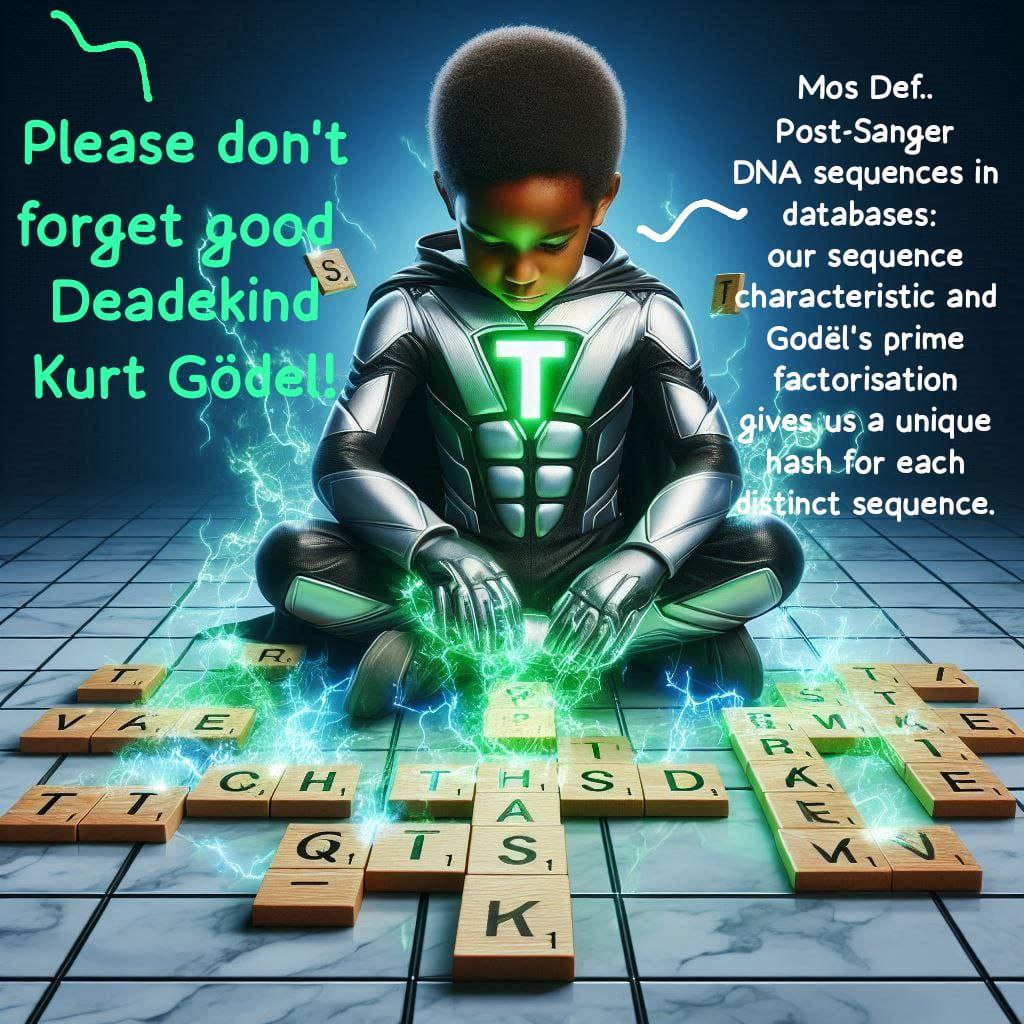
\includegraphics[width=0.9\textwidth,]{resources/images/further_analysis.jpg}\\
   \caption{Some proposal to use G$\ddot{o}$del's idea of abstracting formulae such as formal symbolic sequences using distinct natural numbers.}
  \label{FIGGODELIDEA}
  \end{center}
\end{figure}


$na$-Sequences, for which we might have a collection of them, $\Theta^n$, could have applied to them, a system of optimal or optimizable storage in practice, especially via electronic formats and protocols such as with flat text files, relative database systems and any well structured \textbf{operating memory space structures} --- vaults in TEA\cite{Lutalo2024_taz}, JSON-dictionaries on the Web\cite{lutalo_tea_web}, YAML files on local file-systems, etc. In this section, we could explore with the same na-Sequences introduced in \textbf{\hyperref[SEC4ASEQ]{Section \ref{SEC4ASEQ}}}, for ways how their corresponding optimal hash keys might be computed as part of an optimal-sequence lookup mechanism in bio-automata or not.

Concerning Storage of an na-Sequence $\theta_n \in \Theta^n_k$ such that  $\Theta$ has $n$ sequences partitioned into $k$ subsequences\footnote{This is just the proposed concept of the storage representation for an individual entire genome sequence,  just one of many possibilities. Particular implementations might vary in actual sequence expression (in storage). For nucleic acid operating systems, we know that na-Sequences are in natural storage, when expressed as DNA (with partitions into nucleic acids, codons, genes, chromosomes, double-helixes of chromosomes, etc), however, while in use for processes such as RNA-oriented sequence processing (see \textbf{\hyperref[SECPROT]{Section \ref{SECPROT}}}, are operated on, not in bulk or whole-at-once, but in subsequences of some finite length --- such as $k$ in this formal specification, and $k=3$ for typical, natural protein synthesis in ribosomes as an example.}.

We then might wish to have some mechanism --- such as the following generator:\\


\begin{transf}[A \textbf{Sequence Lookup System}, sLS($Q_m,\Theta^n$)]:
\label{TRANSFSEQLOOKUP}
$ $\\
$\Theta^n \xrightarrow{sLS(Q_m,\Theta^n)} \theta_i;$\\ 
$\invpi(Q_m) = m \leq \invpi(\theta_i) \quad \land \quad (\ddot{o}(Q_k) \approx \ddot{o}(\theta_i) \quad \lor \quad \tilde{A}(\overset{>}{Q_k} \rightarrow \overset{>}{\theta_i}) \leq \epsilon$\\
$\qed$
\end{transf}


By \textbf{\hyperref[TRANSFSEQLOOKUP]{Transformer \ref{TRANSFSEQLOOKUP}}}, we can search for and express or return, a complete na-Sequence $\theta_i \in \Theta^n$, when presented with some query na-sequence $Q_m$ of length $m$.

Thus, for optimal lookup mechanisms --- concerns about space and [polynomial] time for looking up and returning $\theta_{na}$ from some \textbf{na-database}, $D\langle {\theta i}_{key}, {\theta i}_{val} \rangle^*$, such that, instead of directly searching the collection for the sequence with value $\theta_i = {\theta i}_{val} \approx Q_m$, directly/naively using $Q_m$ --- the \textbf{user provided query}, we use the provably shorter --- in terms of storage space, but also [\textit{more intelligent-friendly} --- in terms of sequence-expressing-information] higher \textbf{entropy encoding} structure, such as with a \textbf{hash key} for each $\theta_i$ as well as any $Q_k$, computed as:\\

\begin{equation}
\label{EQHASHKEYSEQ}
 \Gamma (id(\theta_i)) = \ddot{o}(\prod\limits_{\omega_i,f_i \in \hbar(\overset{>}{\theta_i})} \omega_i\cdot f_i) \approx \ddot{o}(\hbar(\overset{>}{R_{\Theta^n_k}}))
\end{equation}\\



 --- see definition of $R_{\Theta^n_k} \approx \Theta_n$ in \textbf{\hyperref[LAWGDL]{IGS Law}}, while the special sequence operator $\ddot{o}(\Theta_n)$ computes and returns a \textbf{G$\ddot{o}$del Number}\cite{illingworth1996computing}\footnote{Based on the concept of \textbf{G$\ddot{o}$del numbering} --- ``A one-to-one mapping (i.e. an injection) of the symbols, formulas, and finite sequences of formulas of the formal system onto some subset of the natural numbers. The mapping must be such that there is an algorithm that, for any symbol, formula, or finite sequence of formulas, identifies the corresponding natural number; this is the \textit{G$\ddot{o}$del number} of that object."\cite{illingworth1996computing}. G$\ddot{o}$del numbers are a method developed by Kurt G$\ddot{o}$del in 1931\cite{godel1931} to encode symbols, formulas, and entire proofs from formal mathematical systems as unique natural numbers. This encoding allows syntactic objects to be treated arithmetically\cite{godel1931english}.}, $\ddot{o}(\Theta_n): \psi_{\Theta_n}^k \times\mathbb{N}^k \rightarrow \mathbb{N}$ that is derived optimally using the characteristic, $\hbar(\overset{>}{\Theta_n})$, for $\Theta$ a sequence of length $n$, and the first $k$ prime numbers such that $k = \invpi(\overset{>}{\Theta_n}) \quad \land \quad \forall \omega_i \in \hbar(\overset{>}{\Theta_n}): \ddot{o}(\omega_i) : \ddot{o}(i) = f_i \times p_i \in \mathbb{P}$ --- $p_i$ is the $i$-th prime\footnote{$\mathbb{P}$ is the set of all prime numbers.} starting from 2 and spanning $\mathbb{N}$.
 
 Computing a hashkey based on a G$\ddot{o}$del number is just one approach to the optimal way to implement a sequence lookup mechanism with \textbf{\hyperref[TRANSFSEQLOOKUP]{Transformer \ref{TRANSFSEQLOOKUP}}}. However, even that method utilizes the transformatics concept of summarizing arbitrary sequences by their [proposed] \textbf{sequence characteristic} and consequently, their \textbf{modal sequence statistic}. However, as we see in the constraints and specification of that generator-transformer, the other option is to compute the solution using keys based on just the modal sequence statistics of the query and the target sequences in $\Theta^n$.


%---refs fixed up to this point...

\chapter{The Mathematics of Genome Sequencing: Sequence Alignment, The Modal Sequence, The Sequencing Machine and the Identifier Genome Sequence Law}
\label{SECMATHSEQ}

Given what we know of genome sequencing theory and some problems we identified --- such as an overall lack of proper mathematical formalism around the issue of how sequencing --- or rather, computation of the resultant, consensus and most representative genome sequence (essentially, an identifying \textbf{na-Sequence}) of a living organism or particular aspects of it --- proteins, mutations, behavioral traits, anomalies or bases of particular or general diseases or incapacities, etc. But even with the matter of mathematically expressing anomalous entities such as viruses and such, wasn't that compelling. And thus this section.

Seeing as the matter of determining the actual na-Sequence that correctly identifies a person or thing might be hinging on the case of attempting to reconstruct a book by mathematically piecing together disparate pieces of it --- some in alignment, some not, some supersets of the others, some prefixes or suffixes of others, etc.\footnote{This analogy shouldn't come as a surprise, when compared to how we found it best to describe DNA using a figurative metaphor (see \textbf{\hyperref[SEC1]{Introduction}}), but also based on how some authorities seem to be teaching this subject to their students\cite{przytycka_wgs_lecture10}.} Also, though we might not immediately surface that philosophy here, the difficulties and problem thus raised, might likewise apply to the matter of trying to computationally ``sequence" all of reality or even peculiar small aspects of it --- sub-atomic particles that make up living things on the miniature scale, and then planets, stars and galaxies on the grand scale. Is it possible? Does it make sense? Is it necessary or even useful? These, and related problems are what we shall attempt to answer in the rest of this section.

\section{PROBLEM G1: Computing Maximum Common Subsequence: $\Theta_1 \Diamond \Theta_2$}
\label{PROBG1}

\begin{prob}[\textit{Computing MCS:}]: $\Theta_1 \Diamond \Theta_2$] 
\label{PROBMCS}
Given sequences $\Theta_1 = \langle k, l, m, o, p, x, y, z \rangle$ and $\Theta_2 = \langle b, c, a, y, z, k, l, m, o, p \rangle$, find the longest common subsequence they share --- also to be denoted $\Theta_1 \Diamond \Theta_2$, their \textbf{M}aximum \textbf{C}ommon \textbf{S}ubsequence.

\begin{soln}
\label{SOLMCS}
We shall specify a transformer, tMCS($\Theta_1,\Theta_2$) that produces the required solution from the input sequences as such:

\begin{transf}[The \textbf{tMCS} Transformer]
\label{TRANSFMCS}
$\langle \Theta_1,\Theta_2 \rangle  \quad \xrightarrow{O_{tMCS}(\Theta_1,\Theta_2)} \quad \Theta_1 \Diamond \Theta_2;$\\
$0 \leq \invpi(\Theta_1 \Diamond \Theta_2) \leq Max(\invpi(\Theta_1), \invpi(\Theta_2))$
\end{transf}
$\qed$
\end{soln}
\end{prob}

\textbf{\hyperref[SOLMCS]{Solution \ref{SOLMCS}}} is easier said than done. However, we shall attempt to formally and rigorously express it by formalizing what exactly the $tMCS(\Theta_1,\Theta_2)$ transformer does. Basically, we are to compute the MCS via \textbf{\hyperref[ALGtMCS]{Algorithm \ref{ALGtMCS}}}.


\begin{alg}[The \textbf{tMCS} Algorithm]
\label{ALGtMCS}
\begin{enumerate}
\item{Initialize the global maximum common sequence, $O^m_g$, to the empty set.} 
\item{
Given \textbf{a collection of $n$ sequences}, $\Theta^n = \{\Theta_1, \Theta_2,...\}$.
}
\item{
Start by computing the cardinality of each sequence, $\Theta_i \in \Theta^n$, and note the \textbf{largest sequence cardinality}, $Max(\invpi(\Theta_i) \forall \Theta_i \in \Theta^n)$ = $Max(\invpi(\Theta_i))$, for the longest sequence, $\Theta_m$ such that $Max(\invpi(\Theta_i)) = \invpi(\Theta_m)$.
}
\item {
Compute the cardinality of a sequence that can exactly contain the given sequences each concatenated to the other, but with the longest sequence duplicated. Essentially, compute:

\begin{equation}
\label{EQLSEQ}
C_R = \invpi(\Theta_m) + \sum\limits_{\forall \Theta_i \in \Theta^n} \invpi(\Theta_i)
\end{equation}

}
\item{
Sort the collection of sequences, $\Theta^n$, in ascending order of the sequence cardinality. Let the sorted sequence collection be denoted ${\hat{\Theta}}^n$
}
\item {
Start with the first two sequences from ${\hat{\Theta}}^n$, such as $\Theta_1$ and $\Theta_2$, and place them within two adjacent arrays $A_1^{C_R}$ and $A_2^{C_R}$ of equal length $C_R$ --- for simplicity, we shall just denote them as  $A_1$ and $A_2$, in such a way that $\Theta_1$ occupies in its containing array $A_1$, positions from 1 to $\invpi(\Theta_1)$, while $\Theta_2$ occupies positions in the range: $[(1 + \sum \limits_{\Theta: \invpi(\Theta) > \invpi(\Theta_2)}\invpi(\Theta)) = I(\Theta_2[1] \in A_2)$\footnote{We write $\Theta_2[1]$ to mean the first element in $\Theta_2$ --- i.e. position 1 has value 1, and the nth position has value $n$, not usual $n-1$}, $I(\Theta_2[1] \in A_2) + \invpi(\Theta_2) - 1]$, which also means, $\forall a_i \in \Theta_j$ such that $I(\Theta_j,\hat{\Theta}_n) <  I(\Theta_2, \hat{\Theta}_n)$, it implies $j < I(\Theta_2[1] \in A_2)$.

And Equivalently, the range $[\invpi(\Theta_1)+1, \invpi(\Theta_1)+ 1 \invpi(\Theta_2) - 1] = [\invpi(\Theta_1)+1, \invpi(\Theta_1)+ \invpi(\Theta_2)]$. 

Visually, we can express this as:\\\\

\begin{tabular}[H]{|c||c|c|c|c|c|c|c|c|c|c|}
\hline
$A_1$ & $a_{1,1}$ & $a_{1,2}$ & $\cdot\cdot\cdot$ & $a_{1,\invpi(\Theta_1)}$ & & & & & & \\
\hline
$A_2$ & & & & & $a_{2,1}$ & $a_{2,2}$ & $\cdot\cdot\cdot$ & $a_{2,\invpi(\Theta_1)}$ & & \\
\hline
 
\end{tabular}\\\\


}
\item{
Update the two sequence alignment arrays as such:
\begin{enumerate}
\item{
Keep the first array, $A_1$, unchanged (since it contains the longest sequence, $\Theta_1 \in \hat{\Theta}_n$).
}
\item Set $j = z$, where $z$ is the \textbf{shift step size} --- simplest scenario, $z = 1$.
\item {Shift each element in the second sequence by $z$-steps to an earlier position in array $A_2$, so that the two sequences $\Theta_1$ and $\Theta_2$ have an overlap across the alignment arrays/matrix in positions spanning range: $[\invpi(\Theta_1)+1-j, \invpi(\Theta_1)]$, and so that $\Theta_2$ shall be occupying the updated range: $[\invpi(\Theta_1)+1 - j, \invpi(\Theta_1)+\invpi(\Theta_2) - j]$}
\item {
Scan the overlapping sections in both sequences, in positions  $[\invpi(\Theta_1)+1-j, \invpi(\Theta_1)]$, and by comparing each item in that range --- i.e. $\Theta_1[i]$ Vs $\Theta_2[i]$, determine the longest common subsequence, or rather the \textbf{MCS}, thus:\\

Assume the overlap is of length $m$ such that the overlap can be visually depicted as such:\\\\

\begin{tabular}[H]{|c||c|c|c|c|}
\hline
$\approx \Theta_1$ & $a_{1,k}$ & $a_{1,k+1}$ & $\cdot\cdot\cdot$ & $a_{1,k+m}$\\
\hline
$\approx \Theta_2$ & $a_{2,l}$ & $a_{2,l+1}$ & $\cdot\cdot\cdot$ & $a_{2,l+m}$\\
\hline
$(\Theta_1[i] == \Theta_2[i])?$ & 1 & 0 &  $\cdot\cdot\cdot$ & 1\\
\hline
$\approx (\Theta_1[i] == \Theta_2[i]) \approx O^m$ & $f(a_{1,k},a_{2,l})$ & 0 &  $\cdot\cdot\cdot$ & $f(a_{1,k+m},a_{2,l+m})$ \\
\hline
 \end{tabular}\\\\
 
 for some $k \in [1,\invpi(\Theta_1)]$ and $l \in [1,\invpi(\Theta_2)]$.
 
 Create another array of maximum length $m$, $O^m$, which contains at most m elements generated thus:
 \begin{itemize}
 \item $O^m[i]$ contains 0 if the corresponding two elements in $\Theta_1$ and $\Theta_2$ didn't match. Otherwise it contains the matching element value from the first sequence --- or rather, $f(a_{1,k},a_{2,l}) = a_{1,k}$ iff $a_{1,k} == a_{2,l}$.
 \item truncate $O^m$ to its longest non-zero/non-empty subsequence, set that as $O^m$.
 \item Iff $\invpi(O^m) > \invpi(O^m_g)$, then \textbf{Update} or replace $O^m_g$ with $O^m$\\ $\implies$  $O^m_g := O^m$
 \end{itemize}
}
\item{
Update $j \implies j := j + z$
}
\item {
Iff $j = \invpi(\Theta_2)$, then return $O^m_g$
}
\item{Otherwise Iterate from \textbf{Step\#c}}
\end{enumerate}
}
\end{enumerate}
\end{alg}


\section{PROBLEM G2: Computing Overlap Resultant Sequences: $\Theta_1 \ast \Theta_2$}
\label{PROBG2}

\begin{prob}[\textit{Computing ORS: \textbf{Overlap Resultant Sequence}}]: $\Theta_1 \ast \Theta_2$] 
\label{PROBORS}
Given two overlapping/well-aligned sequences $\Theta_1$ and $\Theta_2$ of the same length but potentially different terms at any position in the range $[1, \invpi(\Theta_1)]$, how to compute a resultant sequence $\Theta_1 \ast \Theta_2$ that is most meaningful for DNA sequences?

\begin{soln}
\label{SOLORS}
Assuming $\Theta_1 = \langle \prod\limits_{i=1}^n a_i, \rangle$ and $\Theta_2 = \langle \prod\limits_{i=1}^n b_i, \rangle$, construct $\Theta^*$ via the following tORS transformer:

\begin{transf}[The \textbf{tORS} Transformer]$ $\\
\label{TRANSFORS}
$\langle\langle \Theta_1\langle \prod\limits_{i=1}^n a_i, \rangle, \Theta_2\langle \prod\limits_{i=1}^n b_i, \rangle \rangle  \quad \xrightarrow{O_{tORS}(\Theta_1,\Theta_2)} \quad \Theta^* = 	 \quad \Theta_1 \ast \Theta_2;$\\
$\invpi(\Theta_1 \ast \Theta_2) = \invpi(\Theta_1) = \invpi(\Theta_2) = n$\\
$\land \quad \Theta^* = \langle \prod\limits_{i=1}^n f(a_i,b_i), \rangle$\\
 for $f(x,y)$ \textbf{a resolver function} defined as such:

\[
f(x,y) = 
\begin{cases}
x, & x == y, \text{terms are the same}\\
x, & x = \lnot(y), \text{one term is the complement of the other}\\
y & otherwise.
\end{cases}
\]

\end{transf}
$\qed$
\end{soln}
\end{prob}

\section{PROBLEM G3: Computing the Genome Sequence (GS): $(\Theta_1 \Diamond \Theta_2)^*$}
\label{SECCOMPGENSEQ}

\begin{prob}[\textit{Computing GS: \textbf{Genome Sequence}}]: $(\Theta_1 \Diamond \Theta_2)^*$] 
\label{PROBGS}
Given any two sequences, $\Theta_1$ and $\Theta_2$, compute their \textbf{resultant genome sequence}, denoted $(\Theta_1 \Diamond \Theta_2)^*$, that contains at core, their longest common subsequence (the MCS), $O^m = (\Theta_1 \Diamond \Theta_2)$, potentially padded either side by the specially computed prefix and suffix subsequences from either input sequence as such:\\

\begin{equation}
\label{EQGS}
(\Theta_1 \Diamond \Theta_2)^* \quad = \quad \Theta_1^a\cdot(\Theta_1^b \ast \Theta_2^b)\cdot(\Theta_1 \Diamond \Theta_2)\cdot(\Theta_1^c \ast \Theta_2^c)\cdot\Theta_2^a\\\\
\end{equation}

And where the special terms are derived and named as such:

\begin{itemize}
\item $\Theta_1^a$ is the non-overlapping section of $\Theta_1$ before the \textbf{COS}.
\item $(\Theta_1^b \ast \Theta_2^b)$ is the consensus sequence from $\Theta_1$ and $\Theta_2$ such that its elements are the result of applying the \textbf{resolver function} to compute $f(\Theta_1[i],\Theta_2[i])$ as specified in \textbf{Transformer \ref{TRANSFMCS}}. It occurs \textbf{before the MCS}.
\item $(\Theta_1 \Diamond \Theta_2)$ is the \textbf{maximum common subsequence}, MCS, $O^m_g$, of $\Theta_1$ and $\Theta_2$. It is the heart of the computed genome sequence.
\item $(\Theta_1^c \ast \Theta_2^c)$ is the consensus sequence from $\Theta_1$ and $\Theta_2$ \textbf{after the MCS}.
\item  $\Theta_2^a$ is the non-overlapping section of $\Theta_2$ after the \textbf{COS}.
\end{itemize}

\textbf{COS}, $\overline{\Theta_1\Theta_2}$, which is the \textbf{Consensus Overlapping Sequence}, padded on either by the non-overlapping sections of either $\Theta_1$ or $\Theta_2$, has the following properties:

\begin{itemize}
\item $\overline{\Theta_1\Theta_2} = (\Theta_1^b \ast \Theta_2^b)\cdot(\Theta_1 \Diamond \Theta_2)\cdot(\Theta_1^c \ast \Theta_2^c)$
\item $\Theta_1 \approx \Theta_1^a \cdot \overline{\Theta_1\Theta_2}$
\item $\Theta_2 \approx \overline{\Theta_1\Theta_2} \cdot \Theta_2^a$
\end{itemize}

So that we could rewrite \textbf{Equation \ref{EQGS}} as such:

\begin{equation}
\label{EQGS2}
(\Theta_1 \Diamond \Theta_2)^* \quad = \quad \Theta_1^a\cdot\overline{\Theta_1\Theta_2}\cdot\Theta_2^a\\\\
\end{equation}

Finally, we know that the cardinality of the genome sequence, $\invpi((\Theta_1 \Diamond \Theta_2)^*)$, is bounded thus:

\begin{equation}
\label{EQBOUNDGS}
\invpi(\Theta_m) \leq \invpi((\Theta_1 \Diamond \Theta_2)^*) \leq \invpi(\Theta_m) + \sum\limits_{\forall \Theta_i \in \Theta^n} \invpi(\Theta_i)
\end{equation}

As per \textbf{Equation  \ref{EQLSEQ}} and the sensibilities of GTNC\cite{Lutalo2024gtnc}.

\end{prob}

\section{The Genome Sequencer}
\label{SECGENSEQ}

\fbox{\begin{minipage}{0.9\textwidth}
\begin{defn}[A \textbf{Genome Sequencer}]
\label{DEFGENOMESEQ} 
A solution to \textbf{Problem \ref{PROBGS}}, is a special sequence processor, $\tilde{T}(\Theta^n)$, that can compute and return a resultant sequence, $R_{\Theta^n}$, also known as the \textbf{genome sequence}, defined as\footnote{Note that, even though in our formalism here we express the \textbf{relative complement set} of $\{\Theta_m\}$ in $\Theta^n$ as $\Theta^n \setminus \Theta_m$ --- especially to keep the notation simple, we actually mean $\Theta^n \setminus \{\Theta_m\}$, which means, the first set with the elements in the second set omitted.}

\begin{equation}
\label{EQGSVAL}
R_{\Theta^n} = (\Theta_m \Diamond \Theta^n \setminus \Theta_m)^* 
\end{equation}

Such that $\Theta_m$ is the longest sequence in $\Theta^n$ --- a collection of $n$ sequences, and that $\tilde{T}(\Theta^n)$ produces/generates/computes $R_{\Theta^n}$ by iteratively computing and updating the genome sequence in n-1 iterations as such:

\begin{trans}
\label{TRANSGENSEQ}
$R_{\Theta^n}^0 \xrightarrow{O_{tGS}(\{R_{\Theta^n}^0\} \cup\Theta^n,0)} R_{\Theta^n}^1$
$\xrightarrow{O_{tGS}(\{R_{\Theta^n}^1\} \cup \Theta^{n-1},1)} R_{\Theta^n}^2$
$\xrightarrow{O_{tGS}(\{R_{\Theta^n}^2\} \cup \Theta^{n-2},2)}$
$\ldots \xrightarrow{O_{tGS}(\{R_{\Theta^n}^j\} \cup \Theta^{n-j},j)} R_{\Theta^n}^{j+1}$
$\ldots \xrightarrow{O_{tGS}(\{R_{\Theta^n}^{n-2}\} \cup \Theta^{1},n-2)} R_{\Theta^n}^{n-1}$
\end{trans}

To produce the final genome sequence, $R_{\Theta^n}^{n-1}$ via the \textbf{tGS Transformer} defined as such:

\begin{transf}[The \textbf{tGS Transformer}, $\tilde{T}(\Theta^n)$]
$R_{\Theta^n}^{j} \xrightarrow{O_{tGS}(\{R_{\Theta^n}^j\} \cup \Theta^{n-j},j)} R_{\Theta^n}^{j+1};$
$R_{\Theta^n}^{0} = \emptyset$\\
and $R_{\Theta^n}^{j+1}$ is the resultant genome sequence after processing $\Theta^n$ with the first $j$ sequences removed from it, and with the previous genome sequence, $\{R_{\Theta^n}^j\}$ appended to it, so as to produce that next genome sequence $R_{\Theta^n}^{j+1}$.
\end{transf} 

\end{defn}
\end{minipage}}
\\

That transformer, $\tilde{T}(\Theta^n)$, is a genome sequencer, and is essentially a transformer that reduces a matrix of na-Sequences to a resultant sequence, $R_{\Theta^n}$, that is the resultant genome sequence of a specie, population, or any natural entity represented by or expressed by the [potentially incomplete or approximate] genome sequences in the collection $\Theta^n$.


\section{The Identity Genome Sequence (IGS) Law}
\label{SECIGSL}

\begin{law}[The \textbf{Identity Genome Sequence Law}]
\label{LAWGDL}
The Identity Genome Sequence, $R_{\Theta^n}(\Omega): \mathbb{N} \times \psi_{DNA}$, derived from some collection of sequences, $\Theta^n \langle \prod\limits^n \theta_i \rangle$ such that $\theta_i \subset \Omega \lor \theta_i \approx \Omega$ are approximations of $\Omega$, the longest known genome sequence of the entity, whose exact genome sequence would be $\Omega$, and which can uniquely identify it. For sufficiently large $n$, and where the sample sequences $\theta_i$ were read or generated correctly by scanning or sequencing the entity, then 

\begin{equation}
\label{SEQRofOM}
R_{\Theta^n}(\Omega) \approx \Omega_m
\end{equation} 

Where $\Omega_m$ is the known best approximation of the genome sequence that correctly identifies any instance of a member of the kind $\Omega$.
\end{law}

\begin{center}
\fbox{\begin{minipage}{0.9\textwidth}
\large
\textbf{NOTE:}\\
 On \textbf{Consequences of IGS} \\

One potentially significant consequence of \textbf{Law \ref{LAWGDL}} is that every distinct living thing --- unique or distinct animal, plant, eukaryote or prokaryote, has a distinct identifying genome sequence, $\Omega$, that we can discover and/or approximate via significantly many readings of particular or representative [sub-]sequences of the DNA of the observable expressions of $\Omega$.

However, given that in reality it might not be exactly possible to exhaustively compute the correct value of $R_{\Theta^n}$, nor tell exactly when that approximation approaches $\Omega$ exactly, it makes one wonder whether we can ever accurately know what it is that exactly underlies the expression of our reality --- living things or not\footnote{Of course, there is the queer possibility that a kind of genome sequencing might be applicable to also inanimate/non-living things! But that's a philosophical discussion for another day.}.

\end{minipage}}
\\
\end{center}




\chapter{Random Sequence Generators (RSGs)}
\label{SECRSG}


In many problems involving intelligent or non-linear processing of sequences, we might come across the need for either a random number, a random symbol or a random sequence of these, spanning some known/particular symbol set. This for example could be how we solve the problem: \textbf{Given the DNA symbol set $\psi_{DNA}$, how to generate a random DNA sequence of length n?}.

So, to help solve such critical and fundamental problems once and for all, and in a generic, transformatic-way, we shall specify some fundamental stochastic generator machines and algorithms, and these can then be used to solve any specific problem of generating a random sequence of a specific length given some finite symbol set.

\section{The First Lu-Shuffle Algorithm (FLSA)}

For this algorithm, for which we shall start by specifying its signature, the most important property it has is that it merely takes a sequence $\Theta$ as input and some parameter $k$ --- that \textbf{should lie in range} $1 \leq k \leq n$ and that $\invpi(\Theta) \geq 2$.

\subsection{The FLSA Algorithm Using Mathematics}

\begin{alg}[The \textbf{First Lu-Shuffle Algorithm}: $\text{flsa}(\Theta, k_0)$]
\label{ALGLUSHUFFLEA}
$ $\\
\begin{enumerate}
\item \textbf{GIVEN} source sequence $\Theta$ of length $n = \invpi(\Theta)$.
\item  \textbf{GIVEN} input parameter $k_0$ that is \textbf{Initial Partition Index}.
\item \textbf{IF} $n < 2$ \textbf{RETURN} $\Theta$ unmodified.
\item {\textbf{LIMIT} initial partition index using cardinality of input sequence, i.e
\begin{equation}
k = k_0 \mod n
\end{equation}
}
\item \textbf{IF} $k < 1$ \textbf{UPDATE}: $k = 1$.
\item{  \textbf{INITIALIZE} the \textbf{resultant sequence}, $\Theta^*$ with $\Theta$.

		\begin{equation}
		\Theta^* = \Theta_{input} = \Theta
		\end{equation}
}
\item { \textbf{WHILE} \textbf{TRUE}:
\begin{enumerate}
	\item \textbf{BREAK IF} $k = n$
	\item \textbf{SET} partition index, $p_{index} = k$
	\item \textbf{SET} partition start, $p_{start} = 0$
	\item \textbf{SET} sub-partition end/index, $sp_{index} = \text{\textbf{CEIL}}(\frac{p_{index}}{2})$
	\item \textbf{SET} left sub-partition, $\Theta_{l} = \{\omega_i | \omega_i \in \Theta^* \quad \land \quad i \in [p_{start},sp_{index}]\}$
	\item \textbf{SET} right sub-partition, $\Theta_{r} = \{\omega_i | \omega_i \in \Theta^* \quad \land \quad i \in [sp_{index},p_{index}]\}$
	\item \textbf{SET} unpartitioned sequence, $\Theta_{rest} = \{\omega_i | \omega_i \in \Theta^* \quad \land \quad i \in [p_{index},n]\}$
	\item \textbf{SET} swapped sequence, $\Theta_{swap} = \Theta_{r} \cdot \Theta_{l}$ 
	
	\item{\textbf{IF} $k$ is \textbf{ODD}: $(k \mod 2) = 1$:
		\begin{enumerate}
			\item \textbf{UPDATE} \textbf{resultant sequence}, $\Theta^* = \Theta_{rest} \cdot \Theta_{swap}$
		\end{enumerate}
	}
	\item{\textbf{ELSE IF} $k$ is \textbf{EVEN}: $(k \mod 2) = 0$:
		\begin{enumerate}
		\item \textbf{UPDATE} \textbf{resultant sequence}, $\Theta^* = \Theta_{swap} \cdot \Theta_{rest}$
		\end{enumerate}
	}
	
	\item \textbf{INCREMENT} $k$: $k = k + 1$
\end{enumerate}
}
\item \textbf{RETURN} resultant sequence, $\Theta^*$.
\end{enumerate}
$\qed$
\end{alg}


\subsection{Examples of Applying FLSA}
\label{SECAPPLYFLSA}

Using the basic, yet important sequence, $\psi_{10}$ (refer to \textbf{\hyperref[EQHYPDNASS]{Equation \ref{EQHYPDNASS}}}) as the input, especially given we leverage such in many aspects of applied transformatics and genetics engineering in this work, we see hereafter, a trace of the accurate \textbf{invariant}\footnote{Basically, for a given particular input sequence such as $\psi_{10}$, we shall \textbf{always} get the same exact resultant sequence for a particular $k$, so that, it feels as though the algorithm randomizes the input sequence, but in a predictable/derivable manner, and this has its relevance in many problems as we shall come to appreciate.} variants (actually, computed and predictable anagrams) of that set --- all of them \textbf{base-10 o-SSIs}\cite{ossipaper}, when it is shuffled using \textbf{\hyperref[ALGLUSHUFFLEA]{Algorithm \ref{ALGLUSHUFFLEA}}} and various \textbf{meaningful values}\footnote{I say ``meaningful" because, given how the algorithm works --- shuffling the input sequence by partitioning it up into chunks and then swapping their order, the partitioning index, which determines where the swapping starts, \textbf{would not make much sense} for values greater than $\frac{\invpi(\Theta)}{2}$, and for values less than $1$. Also, the algorithm doesn't make sense for any value of $k$ when $\invpi(\Theta) \leq 1$. Luckily, the algorithm as specified in \hyperref[ALGLUSHUFFLEA]{Algorithm \ref{ALGLUSHUFFLEA}} is designed so that it checks and applies the necessary remedies for meaningless values of $k$ --- such as setting $k = k \mod n$ for $k > n$ and $k=1$ for $k < 1$. It returns $\Theta$ unmodified for cases where $\invpi(\Theta) \leq 1$.} of the \textbf{initial partition index} $k$, starting from 1 and \textit{preferably} up to $\frac{n}{2} = 5$ --- we have also included values up to $n-1$, just to drive the point home, that the algorithm shall return a result with some \textbf{k-grams}\footnote{The more common term is usually ``n-grams"} of up to $k = \frac{n}{2}$ in the result for any $k > \frac{n}{2}$ --- those large unshuffled subsequences might spoil the randomness of the resultant as you shall see when inspecting the examples we present. 

\begin{figure}[H]
  \begin{center}
\Large
\begin{verbatim}
GIVEN s=[0, 1, 2, 3, 4, 5, 6, 7, 8, 9]
k=0 | s=[9, 7, 4, 0, 5, 3, 8, 2, 1, 6]
k=1 | s=[9, 7, 4, 0, 5, 3, 8, 2, 1, 6]
k=2 | s=[8, 6, 3, 9, 4, 2, 7, 1, 0, 5]
k=3 | s=[8, 6, 3, 9, 4, 2, 7, 0, 1, 5]
k=4 | s=[5, 3, 0, 6, 1, 7, 4, 8, 9, 2]
k=5 | s=[5, 1, 2, 6, 3, 7, 4, 8, 9, 0]
k=6 | s=[0, 8, 9, 1, 5, 2, 6, 3, 4, 7]
k=7 | s=[3, 8, 9, 4, 2, 5, 6, 0, 1, 7]
k=8 | s=[9, 1, 2, 3, 8, 4, 5, 6, 7, 0]
k=9 | s=[9, 5, 6, 7, 8, 0, 1, 2, 3, 4]
\end{verbatim}

   \caption{A Tabulation Trace of Shuffling the Base-10 n-SSI Sequence with increasing values of $k$, the \textbf{Initial Partitioning Index} for \textbf{\hyperref[ALGLUSHUFFLEA]{Algorithm \ref{ALGLUSHUFFLEA}}}, the \textbf{First Lu-Shuffle Algorithm}.}
  \label{FIGTRACEFLSA}
  \end{center}
\end{figure}


\begin{figure}[H]
  \begin{center}
\Large
\begin{verbatim}

GIVEN s=[1, 2]
k=0 | s=[2, 1]
k=1 | s=[2, 1]


GIVEN s=[1, 2, 3]
k=0 | s=[3, 2, 1]
k=1 | s=[3, 2, 1]
k=2 | s=[2, 1, 3]


GIVEN s=[1, 2, 3, 4]
k=0 | s=[1, 4, 3, 2]
k=1 | s=[1, 4, 3, 2]
k=2 | s=[4, 3, 2, 1]
k=3 | s=[4, 3, 1, 2]
\end{verbatim}

   \caption{A Tabulation Trace of Shuffling basic base-case scenarios to help highlight how \textbf{FLSA} works.}
  \label{FIGTRACEFLSASIMPLE}
  \end{center}
\end{figure}



\textbf{NOTE} that, after looking at the examples in \textbf{\hyperref[FIGTRACEFLSA]{Figure \ref{FIGTRACEFLSA}}} and \textbf{\hyperref[FIGTRACEFLSASIMPLE]{Figure \ref{FIGTRACEFLSASIMPLE}}}, one might somewhat start to comfortably say that the \textbf{best range} for the partitioning index $k$, is possibly $1 \leq k \leq \frac{n}{4}$.

We might also want to look at cases of generating shuffled or randomized na-Sequences based on well-known, useful starter sequences (not necessarily symbol sets, or deduplicated sequences, but still useful). For example, $\Theta_{2na}$ from \textbf{\hyperref[EQDUPLNASEQ]{Equation \ref{EQDUPLNASEQ}}}

\begin{figure}[H]
  \begin{center}
\Large
\begin{verbatim}
GIVEN s=['A', 'C', 'G', 'T', 'U', 'A', 'C', 'G', 'T', 'U']
k=0 | s=['U', 'G', 'U', 'A', 'A', 'T', 'T', 'G', 'C', 'C']
k=1 | s=['U', 'G', 'U', 'A', 'A', 'T', 'T', 'G', 'C', 'C']
k=2 | s=['T', 'C', 'T', 'U', 'U', 'G', 'G', 'C', 'A', 'A']
k=3 | s=['T', 'C', 'T', 'U', 'U', 'G', 'G', 'A', 'C', 'A']
k=4 | s=['A', 'T', 'A', 'C', 'C', 'G', 'U', 'T', 'U', 'G']
k=5 | s=['A', 'C', 'G', 'C', 'T', 'G', 'U', 'T', 'U', 'A']
k=6 | s=['A', 'T', 'U', 'C', 'A', 'G', 'C', 'T', 'U', 'G']
k=7 | s=['T', 'T', 'U', 'U', 'G', 'A', 'C', 'A', 'C', 'G']
k=8 | s=['U', 'C', 'G', 'T', 'T', 'U', 'A', 'C', 'G', 'A']
k=9 | s=['U', 'A', 'C', 'G', 'T', 'A', 'C', 'G', 'T', 'U']
\end{verbatim}

   \caption{A Tabulation Trace of Shuffling the na-Sequence $\Theta_{2na}$ from \textbf{\hyperref[EQDUPLNASEQ]{Equation \ref{EQDUPLNASEQ}}} with \textbf{\hyperref[ALGLUSHUFFLEA]{Algorithm \ref{ALGLUSHUFFLEA} (FLSA)}}.}
  \label{FIGTRACEFLSA2NA}
  \end{center}
\end{figure}

A closely related set of random na-Sequences would be that generated with \textbf{\hyperref[ALGLUSHUFFLEA]{Algorithm \ref{ALGLUSHUFFLEA}}} from the palindrome sequence $\Theta_{palna}$ from \textbf{\hyperref[EQPALNASEQ]{Equation \ref{EQPALNASEQ}}}:


\begin{figure}[H]
  \begin{center}
\Large
\begin{verbatim}
GIVEN s=['A', 'C', 'G', 'T', 'U', 'U', 'T', 'G', 'C', 'A']
k=0 | s=['A', 'G', 'U', 'A', 'U', 'T', 'C', 'G', 'C', 'T']
k=1 | s=['A', 'G', 'U', 'A', 'U', 'T', 'C', 'G', 'C', 'T']
k=2 | s=['C', 'T', 'T', 'A', 'U', 'G', 'G', 'C', 'A', 'U']
k=3 | s=['C', 'T', 'T', 'A', 'U', 'G', 'G', 'A', 'C', 'U']
k=4 | s=['U', 'T', 'A', 'T', 'C', 'G', 'U', 'C', 'A', 'G']
k=5 | s=['U', 'C', 'G', 'T', 'T', 'G', 'U', 'C', 'A', 'A']
k=6 | s=['A', 'C', 'A', 'C', 'U', 'G', 'T', 'T', 'U', 'G']
k=7 | s=['T', 'C', 'A', 'U', 'G', 'U', 'T', 'A', 'C', 'G']
k=8 | s=['A', 'C', 'G', 'T', 'C', 'U', 'U', 'T', 'G', 'A']
k=9 | s=['A', 'U', 'T', 'G', 'C', 'A', 'C', 'G', 'T', 'U']
\end{verbatim}

   \caption{A Tabulation Trace of Shuffling the na-Sequence $\Theta_{palna}$ from \textbf{\hyperref[EQPALNASEQ]{Equation \ref{EQPALNASEQ}}} with \textbf{\hyperref[ALGLUSHUFFLEA]{Algorithm \ref{ALGLUSHUFFLEA} (FLSA)}}.}
  \label{FIGTRACEFLSAPALNA}
  \end{center}
\end{figure}

\subsection{The Source Code for FLSA}

And the essential source code --- compartible with \textbf{Python 3}, is as provided in \textbf{\hyperref[LST_FLSA]{Listing \ref{LST_FLSA}}}


\begin{figure}[H]
  \begin{center}
  \begin{lstlisting}[caption={The FLSA}, label={LST_FLSA}, language=Python, frame=single, numbers=left, basicstyle=\ttfamily,  commentstyle=\color{blue}]
#!/usr/bin/env python3
import math

def lu_shuffler_a(s, k0):
    n = len(s)
    if n < 2:
        return s,k0 #essentially, nothing to shuffle
    # make k meaningful...
    k = k0 % n
    k1 = k # for tracing/debugging...
    k = 1 if k < 1 else k # can't partition between nothing
    new_s = s
    while True:
        if k == n: #can't partition between nothing
            break
        p_index = k
        p_start = 0
        sub_p_index = math.ceil(0.5 * p_index)
        #print(f"At k={k} |"
        #        +f" [[{p_start}-{sub_p_index}][{sub_p_index}-"
        #        +f"{p_index}][{p_index}-{n}]")
        sub_p_l = new_s[p_start:sub_p_index]
        sub_p_r = new_s[sub_p_index:p_index]
        rest_p = new_s[p_index:n]
        swapped = sub_p_r + sub_p_l # first swap
        if k%2 == 1: # k is odd
            new_s = rest_p + swapped # second swap
            #print(f"At k={k} s -->"
            #+f"[{p_index}-{n}][{sub_p_index}-"
            #+f"{p_index}][{p_start}-{sub_p_index}] == {new_s}")
        else:
            new_s = swapped + rest_p # soft swap
            #print(f"At k={k} s --> [{sub_p_index}-"
            #        +f"{p_index}][{p_start}-"
            #        +f"{sub_p_index}][{p_index}-{n}] == {new_s}")
        k += 1 # so we advance from k-gram to (k+1)-grams
    #print(f"k={k1} | s={new_s}")
    return new_s,k

#---[ Uncomment Lines Below to Run Examples ]
#---[Some Further Experiments]
#s = [1,2,3] # a good base-case scenario..
#s = [0,1,2,3,4,5,6,7,8,9] # the base-10 n-SSI
#s = ['A','C','G','T','U','A','C','G','T','U'] # na-SS+na-SS
#s = ['A','C','G','T','U','U','T','G','C','A'] # na-SS+complement(na-SS)
#---[Generate Lu-Shuffle Look-Up Tables]
#k = len(s)
#s_k = 0
#print(f"GIVEN s={s}")
#while s_k < k:
#    lu_shuffler_a(s,s_k) # for FLSA
#    s_k += 1
\end{lstlisting}
  \end{center}
  \caption{The First Lu-Shuffle Algorithm implemented using Python}
\end{figure}


Concerning the source code sample for the \textbf{FLSA} as shown in \textbf{\hyperref[LST_FLSA]{Listing \ref{LST_FLSA}}}, realize that we have chosen to leave explanatory notes and debugging/tracing code (though commented out) within the sample, mostly to help newcomers learn to read the program well as well as help any nonbelievers or critics of the \textbf{FLSA} to try it out themselves and also look at what happens in the guts of the algorithm while it computes the final resultant. This shall help many to also be able to apply or use the algorithm by paper and pen because it is that simple, though unimaginably powerful.


\section{The Second Lu-Shuffle Algorithm (SLSA)}
\label{APPSLSA}

This second algorithm, is a variation of and enhancement of the \textbf{\hyperref[ALGLUSHUFFLEA]{Algorithm \ref{ALGLUSHUFFLEA}}}. Also, and \textbf{IMPORTANT to NOTE}, this second algorithm combines with the first algorithm at each invocation, so that it takes the output of \textbf{FLSA} and further transforms it to produce the (\textbf{\textit{more} randomized}) resultant  sequence as we see in the following algorithm specification:

\subsection{The SLSA Algorithm Using Mathematics}

\begin{alg}[The \textbf{Second Lu-Shuffle Algorithm}: $\text{slsa}(\Theta, k_0)$]
\label{ALGLUSHUFFLEB}
$ $\\
\begin{enumerate}
\item \textbf{GIVEN} source sequence $\Theta$ of length $n = \invpi(\Theta)$.
\item  \textbf{GIVEN} input parameter $k_0$ that is \textbf{Initial Partition Index}.
\item \textbf{IF} $n < 2$ \textbf{RETURN} $\Theta$ unmodified.
\item {\textbf{LIMIT} initial partition index using cardinality of input sequence, i.e
\begin{equation}
k = k_0 \mod n
\end{equation}
}
\item \textbf{IF} $k < 1$ \textbf{UPDATE}: $k = 1$.
\item{  \textbf{INITIALIZE} the shuffled sequence, $\Theta^*$ with the output of invoking \textbf{\hyperref[ALGLUSHUFFLEA]{Algorithm \ref{ALGLUSHUFFLEA}}} using the given parameters as such:

		\begin{equation}
		\label{EQIPI}
		\Theta^*,k^* = \text{lu\_shuffler\_a}(\Theta, n - k)
		\end{equation}
		
		\textbf{IGNORE} $k^*$, while $\Theta^*$ becomes the \textbf{initial shuffled resultant sequence} for the rest of this algorithm.
}
\item { \textbf{WHILE} \textbf{TRUE}:
\begin{enumerate}
	\item \textbf{BREAK IF} $k = n$
	\item \textbf{SET} partition index, $p_{index} = k$
	\item \textbf{SET} partition start, $p_{start} = 0$
	\item \textbf{SET} sub-partition end/index, $sp_{index} = \text{\textbf{CEIL}}(\frac{p_{index}}{2})$
	\item \textbf{SET} left sub-partition, $\Theta_{l} = \{\omega_i | \omega_i \in \Theta^* \quad \land \quad i \in [p_{start},sp_{index}]\}$
	\item \textbf{SET} right sub-partition, $\Theta_{r} = \{\omega_i | \omega_i \in \Theta^* \quad \land \quad i \in [sp_{index},p_{index}]\}$
	\item \textbf{SET} unpartitioned sequence, $\Theta_{rest} = \{\omega_i | \omega_i \in \Theta^* \quad \land \quad i \in [p_{index},n]\}$
	\item \textbf{SET} swapped sequence, $\Theta_{swap} = \Theta_{r} \cdot \Theta_{l}$ 
	
	\item{\textbf{IF} $k$ is \textbf{ODD}: $(k \mod 2) = 1$:
		\begin{enumerate}
			\item \textbf{UPDATE} \textbf{resultant sequence}, $\Theta^* = \Theta_{rest} \cdot \Theta_{swap}$
		\end{enumerate}
	}
	\item{\textbf{ELSE IF} $k$ is \textbf{EVEN}: $(k \mod 2) = 0$:
		\begin{enumerate}
		\item \textbf{UPDATE} \textbf{resultant sequence}, $\Theta^* = \Theta_{swap} \cdot \Theta_{rest}$
		\end{enumerate}
	}
	
	\item \textbf{INCREMENT} $k$: $k = k + 1$
\end{enumerate}
}
\item \textbf{RETURN} resultant sequence, $\Theta^*$.
\end{enumerate}
$\qed$
\end{alg}

So, important to note that \textbf{\hyperref[ALGLUSHUFFLEB]{Algorithm \ref{ALGLUSHUFFLEB}}} invokes \textbf{\hyperref[ALGLUSHUFFLEA]{Algorithm \ref{ALGLUSHUFFLEA}}} with the \textbf{decreasing initial partitioning index} $n-k$ as shown in \textbf{\hyperref[EQIPI]{Equation \ref{EQIPI}}}



\subsection{Examples of Applying SLSA}
\label{SECAPPLYSLSA}



Using the same exact sequences, and in the same order as we utilized in \textbf{\hyperref[SECAPPLYFLSA]{Section \ref{SECAPPLYFLSA}}}, we shall come to appreciate readily, not just that the two algorithms, though they perform similar functions, produce \textbf{different} results for the same exact sequence and same exact partitioning index parameter --- \textbf{IMPORTANT:} However, they are both \textbf{consistent} --- the same input sequence with a particular $k$ shall always produce the expected shuffled sequence post-transform.

Note that \textbf{\hyperref[FIGTRACESLSA]{Figure \ref{FIGTRACESLSA}}} corresponds to the earlier table in \textbf{\hyperref[FIGTRACEFLSA]{Figure \ref{FIGTRACEFLSA}}}.

\begin{figure}[H]
  \begin{center}
\Large
\begin{verbatim}
GIVEN s=[0, 1, 2, 3, 4, 5, 6, 7, 8, 9]
k=0 | s=[4, 2, 8, 9, 0, 7, 3, 6, 5, 1]
k=1 | s=[4, 2, 8, 9, 0, 7, 3, 6, 5, 1]
k=2 | s=[7, 5, 3, 0, 8, 2, 6, 1, 9, 4]
k=3 | s=[1, 6, 4, 7, 2, 9, 0, 3, 8, 5]
k=4 | s=[2, 1, 0, 6, 8, 3, 5, 4, 7, 9]
k=5 | s=[7, 1, 2, 4, 6, 8, 3, 9, 0, 5]
k=6 | s=[5, 9, 2, 3, 7, 0, 4, 6, 1, 8]
k=7 | s=[9, 1, 5, 4, 3, 2, 7, 8, 6, 0]
k=8 | s=[5, 6, 3, 9, 0, 4, 2, 7, 1, 8]
k=9 | s=[6, 3, 8, 2, 1, 9, 7, 4, 0, 5]
\end{verbatim}

   \caption{A Tabulation Trace of Shuffling the Base-10 n-SSI Sequence with increasing values of $k$, using \textbf{\hyperref[ALGLUSHUFFLEB]{Algorithm \ref{ALGLUSHUFFLEB} (SLSA)}}, the \textbf{Second Lu-Shuffle Algorithm}.}
  \label{FIGTRACESLSA}
  \end{center}
\end{figure}


\begin{figure}[H]
  \begin{center}
\Large
\begin{verbatim}

GIVEN s=[1, 2]
k=0 | s=[1, 2]
k=1 | s=[1, 2]


GIVEN s=[1, 2, 3]
k=0 | s=[3, 1, 2]
k=1 | s=[3, 1, 2]
k=2 | s=[2, 3, 1]


GIVEN s=[1, 2, 3, 4]
k=0 | s=[4, 2, 1, 3]
k=1 | s=[4, 2, 1, 3]
k=2 | s=[1, 2, 3, 4]
k=3 | s=[2, 3, 1, 4]
\end{verbatim}

   \caption{A Tabulation Trace of Shuffling basic base-case scenarios to help highlight how \textbf{SLSA} works and how it relates to \textbf{FLSA}.}
  \label{FIGTRACESLSASIMPLE}
  \end{center}
\end{figure}



Note that \textbf{\hyperref[FIGTRACESLSA2NA]{Figure \ref{FIGTRACESLSA2NA}}} corresponds to the earlier table in \textbf{\hyperref[FIGTRACEFLSA2NA]{Figure \ref{FIGTRACEFLSA2NA}}}.


\begin{figure}[H]
  \begin{center}
\Large
\begin{verbatim}
GIVEN s=['A', 'C', 'G', 'T', 'U', 'A', 'C', 'G', 'T', 'U']
k=0 | s=['U', 'G', 'T', 'U', 'A', 'G', 'T', 'C', 'A', 'C']
k=1 | s=['U', 'G', 'T', 'U', 'A', 'G', 'T', 'C', 'A', 'C']
k=2 | s=['G', 'A', 'T', 'A', 'T', 'G', 'C', 'C', 'U', 'U']
k=3 | s=['C', 'C', 'U', 'G', 'G', 'U', 'A', 'T', 'T', 'A']
k=4 | s=['G', 'C', 'A', 'C', 'T', 'T', 'A', 'U', 'G', 'U']
k=5 | s=['G', 'C', 'G', 'U', 'C', 'T', 'T', 'U', 'A', 'A']
k=6 | s=['A', 'U', 'G', 'T', 'G', 'A', 'U', 'C', 'C', 'T']
k=7 | s=['U', 'C', 'A', 'U', 'T', 'G', 'G', 'T', 'C', 'A']
k=8 | s=['A', 'C', 'T', 'U', 'A', 'U', 'G', 'G', 'C', 'T']
k=9 | s=['C', 'T', 'T', 'G', 'C', 'U', 'G', 'U', 'A', 'A']
\end{verbatim}

   \caption{A Tabulation Trace of Shuffling the na-Sequence $\Theta_{2na}$ from \textbf{\hyperref[EQDUPLNASEQ]{Equation \ref{EQDUPLNASEQ}}} with \textbf{\hyperref[ALGLUSHUFFLEB]{Algorithm \ref{ALGLUSHUFFLEB} (SLSA)}}.}
  \label{FIGTRACESLSA2NA}
  \end{center}
\end{figure}


Note that \textbf{\hyperref[FIGTRACESLSAPALNA]{Figure \ref{FIGTRACESLSAPALNA}}} corresponds to the earlier table in \textbf{\hyperref[FIGTRACEFLSAPALNA]{Figure \ref{FIGTRACEFLSAPALNA}}}.



\begin{figure}[H]
  \begin{center}
\Large
\begin{verbatim}
GIVEN s=['A', 'C', 'G', 'T', 'U', 'U', 'T', 'G', 'C', 'A']
k=0 | s=['U', 'G', 'C', 'A', 'A', 'G', 'T', 'T', 'U', 'C']
k=1 | s=['U', 'G', 'C', 'A', 'A', 'G', 'T', 'T', 'U', 'C']
k=2 | s=['G', 'U', 'T', 'A', 'C', 'G', 'T', 'C', 'A', 'U']
k=3 | s=['C', 'T', 'U', 'G', 'G', 'A', 'A', 'T', 'C', 'U']
k=4 | s=['G', 'C', 'A', 'T', 'C', 'T', 'U', 'U', 'G', 'A']
k=5 | s=['G', 'C', 'G', 'U', 'T', 'C', 'T', 'A', 'A', 'U']
k=6 | s=['U', 'A', 'G', 'T', 'G', 'A', 'U', 'T', 'C', 'C']
k=7 | s=['A', 'C', 'U', 'U', 'T', 'G', 'G', 'C', 'T', 'A']
k=8 | s=['U', 'T', 'T', 'A', 'A', 'U', 'G', 'G', 'C', 'C']
k=9 | s=['T', 'T', 'C', 'G', 'C', 'A', 'G', 'U', 'A', 'U']
\end{verbatim}

   \caption{A Tabulation Trace of Shuffling the na-Sequence $\Theta_{palna}$ from \textbf{\hyperref[EQPALNASEQ]{Equation \ref{EQPALNASEQ}}} with \textbf{\hyperref[ALGLUSHUFFLEB]{Algorithm \ref{ALGLUSHUFFLEB} (SLSA)}}.}
  \label{FIGTRACESLSAPALNA}
  \end{center}
\end{figure}

\subsection{The Source Code for SLSA}
\label{SECSLSACODE}

And the essential source code --- compartible with \textbf{Python 3}, is as provided in  \textbf{\hyperref[LST_SLSA]{Listing \ref{LST_SLSA}}}


\begin{figure}[H]
  \begin{center}
  \begin{lstlisting}[caption={The SLSA}, label={LST_SLSA}, language=Python, frame=single, numbers=left, basicstyle=\ttfamily,  commentstyle=\color{blue}]
#!/usr/bin/env python3
import math

def lu_shuffler_b(s, k0):
    n = len(s)
    if n < 2:
        return s,k0
    k = k0 % n
    k1 = k
    k = 1 if k < 1 else k
    new_s = lu_shuffler_a(s,n-k)[0] #invoke FLSA with k0=n-k
    while True:
        if k == n:
            break
        p_index = k
        p_start = 0
        sub_p_index = math.ceil(0.5 * p_index)
        sub_p_l = new_s[p_start:sub_p_index]
        sub_p_r = new_s[sub_p_index:p_index]
        rest_p = new_s[p_index:n]
        swapped = sub_p_r + sub_p_l
        if k%2 == 1:
            new_s = rest_p + swapped
        else:
            new_s = swapped + rest_p
        k += 1
    #print(f"k={k1} | s={new_s}")
    return new_s,k
    
\end{lstlisting}
  \end{center}
  \caption{The Second Lu-Shuffle Algorithm implemented using Python}
\end{figure}


\section{Generating Realistic Random na-Sequences}

In the previous sections we have considered the matter of taking a particular symbol set or some tiny set of almost or exactly distinct symbols and then worked on ways to generate random sequences from these. However, focus was specifically on randomizing an existing sequence, and not necessarily about generating entirely new sequences with say new symbol distributions different from what was in the source/input sequence. Thus, starting from the fundamental aspect of \textbf{generating a SINGLE RANDOM DNA symbol} --- such as randomly generating one of the DNA-nucleobases from $\psi_{DNA}$ or doing the same for RNA, shall be where our adventures start.

\subsection{How to Generate a Random Nucleotide \& The Random Symbol Generator}

Given that we already have the necessary source symbol sets, the matter for how to generate a single \textbf{random letter} from a particular symbol set shall be as follows --- first, we shall merely define an abstract machine using the notation and semantics of transformatics.\\


%\vspace{5cm}
\fbox{
\begin{minipage}{0.9\textwidth}

\begin{transf}[The \textbf{Random Symbol Generator (RSG)}, $RSG(k,\Theta_n)$]
\label{TRANSFRSG}
$ $\\
$\Theta_n \xrightarrow{O_{RSG}(k,\Theta_n)} \Theta^*_k;$\\
$ \quad \invpi(\Theta^*_k) = k \quad \land \quad  \psi(\Theta^*_k) \subseteq \psi(\Theta)$\\
$\land \quad \forall x,y \in \mathbb{N}, \Omega:N \times \psi_y,$\\\\
$ RSG(x,\Omega) = \text{SELECT}(x,\text{SHUFFLE}(\text{PROTRACT}(\psi_y,k \times 2 \times \invpi(\psi_y))))$\\

Where;\\
\begin{itemize}
\item{$\psi_y = \text{USYMBOLSET}(\Omega)$\\
but in a more robust case, we can also randomize the symbol set to be used in generating the random sequence, by generating $\psi_y$ thus:

\begin{equation}
\psi_y = \text{SHUFFLE}(\text{USYMBOLSET}(\Omega))
\end{equation}\\

}
\item \textbf{USYMBOLSET}$(\Omega)$ is a function that reduces the input argument $\Omega$, which is expected to be a sequence of some symbols --- unique or not, to its \textbf{unspecific symbol set} --- $\psi(\Omega)$\footnote{See \textbf{Definition 4} in \cite{ossipaper}}.
\item \textbf{PROTRACT}$(\Theta, n)$ is a transformation of the sequence of [possibly] distinct $n$ symbols from the source sequence $\Theta$ such that the resultant sequence is of length\footnote{But just like the first parameter might be any sequence of symbols, also, the second parameter could be any positive number, and by which, the function shall \textbf{either shrink/truncate or grow/multiply} the input sequence to the required \textbf{multiplier} size} $k \times 2 \times \invpi(\psi_y)$ and spans the source sequence symbol set\footnote{As you shall see in the sample outputs and as well as the actual implementation source code for our \textbf{RSG}, the choice of the protraction parameter $k \times 2 \times \invpi(\psi_y)$, is both to be sensitive to the length of the input sequence's unique symbol set, but also the size of final output required --- both factors influence the quality of the result in terms of randomness/entropy.}.
\item  \textbf{SHUFFLE}$(\Theta)$ is a function such as a generalization of \textbf{lu\_shuffler\_b($\cdot$)} from \textbf{\hyperref[ALGLUSHUFFLEB]{Algorithm \ref{ALGLUSHUFFLEB}}} that returns a shuffled/randomized instance of any input sequence such as $\Theta$ that it is given.
\item \textbf{SELECT}$(x, \Theta)$ is a function that can return the first $x$ terms from $\Theta$ as the result of its invocation for some $x \leq \invpi(\Theta)$.
\end{itemize}
$\qed$
\end{transf}
\end{minipage}}
\\

So, with the essential mathematics out of the way as depicted in \textbf{\hyperref[TRANSFRSG]{Transformer \ref{TRANSFRSG}}}, we can then try to see how this would work practically with some real tangible computer programs that implement that generator-transformer specification.

\subsection{The USYMBOLSET Function}

We shall go bit by bit. So first, here is what the \textbf{USYMBOLSET} function looks like in Python:

\begin{figure}[H]
  \begin{center}
  \begin{lstlisting}[caption={The USYMBOLSET}, label={LST_USYMBOLSET}, language=Python, frame=single, numbers=left, basicstyle=\ttfamily,  commentstyle=\color{blue}]
#!/usr/bin/env python3

#---[ USYMBOLSET(s) ]
def usymbolset(s):
    n_s = len(s)
    if n_s <= 1:
        return s

    # the next commented-out code would kinda work,
    # if we just wanted a dirty and pythonic solution, but 
    # it doesn't respect order of first occurrence!
    #resultant = list(set(s))
 
    #our CORRECT solution for unspecific symbol set.. 
    resultant = []
    for i in range(n_s):
        s_i = s[i]
        if not (s_i in resultant):
            resultant.append(s_i)
    return resultant

#---[ TEST USYMBOLSET ]
#s = [0,1,2,3,4,5,6,7,8,9]
# s = [0,1,2,3,4,5,6,7,8,9] --> usymbolset(s+s+s+s) 
#--> [0, 1, 2, 3, 4, 5, 6, 7, 8, 9]
#s = [1,0,1,1,1,1,1,0,1,1] --> usymbolset(s) --> [0,1]
#s = "3.1415926535898" # --> usymbolset(s) --> 
#['3', '.', '1', '4', '5', '9', '2', '6', '8']
#s = ['A' , 'C' , 'G' , 'T' , 'U' , 'U' , 'T' , 'G' , 'C' , 'A'] #w/duplication
# usymbolset(s) --> ['A', 'C', 'G', 'T', 'U']
#result = usymbolset(s)
#print(result)
\end{lstlisting}
  \end{center}
  \caption{The \textbf{USYMBOLSET}$(\Omega)$ unspecific symbol set generator implemented using Python}
\end{figure}


\subsection{The PROTRACT Function}

We shall go bit by bit. So first, here is what the \textbf{PROTRACT} function looks like in Python:

\begin{figure}[H]
  \begin{center}
  \begin{lstlisting}[caption={The PROTRACT}, label={LST_PROTRACT}, language=Python, frame=single, numbers=left, basicstyle=\ttfamily,  commentstyle=\color{blue}]
#!/usr/bin/env python3
import math

#---[ PROTRACT(s,n) ]
def protract(s,n):
    n_s = len(s)
    if n_s < 1:
        return s
    if n < n_s:
        return s[:n]
    if n == n_s:
        return s
    multiple = math.ceil(n_s / n)
    target_n = n * multiple
    resultant = s
    i = 1
    while i < target_n:
        resultant = resultant + s
        i += 1
    return resultant[:n]

#---[ TEST PROTRACT ]
# s = [0,1,2,3,4,5,6,7,8,9], n = 3 --> [0,1,2]
# s = [0,1,2,3,4,5,6,7,8,9], n = 23 -->
# [0, 1, 2, 3, 4, 5, 6, 7, 8, 9, 0, 1, 2, 3, 4, 5, 6, 7, 8, 9, 0, 1, 2]
#result = protract(s,23)
#print(result)
\end{lstlisting}
  \end{center}
  \caption{The \textbf{PROTRACT}$(\psi_y, 2x)$ sequence generator-transformer implemented using Python}
\end{figure}


\subsection{The Random Number Generator, RNG Function}

Before we proceed to the \textbf{SHUFFLE} function, we shall want to first specify and test an important utility that would otherwise make our implementation dependent on someone else's random sequence generator --- thus rendering all our efforts here almost useless!

The critically important function is \textbf{RNG}$(ll,ul)$ that essentially takes two parameters --- $ll$, the \textbf{lower limit} and $ul$, the \textbf{upper limit}, both of which are expected to be integers, and using which, the function is supposed to generate a \textbf{random number} $n$ that lies within the range:

\begin{equation}
ll \leq n \leq ul
\end{equation}

It is such a CRITICALLY important routine(see author's earlier work on the matter\cite{lnspaper}), however, for the interests of keeping things simple, for now, we shall settle with a basic implementation that only relies on the \textbf{System Time} functions as our \textbf{source of entropy}\footnote{While, and perhaps in the near future, we continue to seek for theory and practical ways to generate entropy algorithmically --- which might be \textit{futile}, or perhaps implement our own entropy generators interfacing with entropy sources in nature?}.

So, without delving into formally specifying our \textbf{Random Number Generator}, \textbf{RNG} here, the associated definition of this utility as implemented using Python is as follows:

\begin{figure}[H]
  \begin{center}
  \begin{lstlisting}[caption={The RNG}, label={LST_RNG}, language=Python, frame=single, numbers=left, basicstyle=\ttfamily,  commentstyle=\color{blue}]
#!/usr/bin/env python3
import time

#---[ RNG(ll,ul) ]
def random_ng(l,u):
    lu = max(l,u)
    ll = min(l,u)
    lu = lu + 1 if ll == lu else lu
    part_k = 1
    candidates = lu_shuffler_a(list(range(ll,lu+1)),part_k)[0]
    n = len(candidates)
    pick = int(time.time())%n #because we need an entropy source!
    return candidates[pick]

#---[ TEST RNG ]
#for r in [[0,10],[0,1],[0,100],[1900,1999]]:
#    print(f"RNG From {r[0]}-{r[1]} -> {random_ng(r[0],r[1])}")
\end{lstlisting}
  \end{center}
  \caption{The \textbf{RNG}$(ll,ul)$ random number generator implemented using Python}
\end{figure}


We can indeed look at some trace dumps from testing our beautiful RNG and appreciate what a little gem it is!

\begin{figure}[H]
  \begin{center}
  \begin{lstlisting}[caption={A TESTING Our RANDOM NUMBER GENERATOR }, label={LST_RNG}, frame=single, numbers=none, basicstyle=\ttfamily,  commentstyle=\color{blue}, breaklines=true, breakatwhitespace=false]

RNG From 0-10 -> 6
RNG From 0-1 -> 0
RNG From 0-100 -> 56
RNG From 1900-1999 -> 1984

RNG From 0-10 -> 7
RNG From 0-1 -> 1
RNG From 0-100 -> 46
RNG From 1900-1999 -> 1950


k=1 | s=[0, 1, 2, 3, 4, 5, 6, 7, 8, 9, 10]
RNG From 0-10 -> 2

k=1 | s=[0, 1]
RNG From 0-1 -> 1

k=1 | s=[0, 1, 2, 3, 4, 5, 6, 7, 8, 9, 10, 11, 12, 13, 14, 15, 16, 17, 18, 19, 20, 21, 22, 23, 24, 25, 26, 27, 28, 29, 30, 31, 32, 33, 34, 35, 36, 37, 38, 39, 40, 41, 42, 43, 44, 45, 46, 47, 48, 49, 50, 51, 52, 53, 54, 55, 56, 57, 58, 59, 60, 61, 62, 63, 64, 65, 66, 67, 68, 69, 70, 71, 72, 73, 74, 75, 76, 77, 78, 79, 80, 81, 82, 83, 84, 85, 86, 87, 88, 89, 90, 91, 92, 93, 94, 95, 96, 97, 98, 99, 100]
RNG From 0-100 -> 28

k=1 | s=[1900, 1901, 1902, 1903, 1904, 1905, 1906, 1907, 1908, 1909, 1910, 1911, 1912, 1913, 1914, 1915, 1916, 1917, 1918, 1919, 1920, 1921, 1922, 1923, 1924, 1925, 1926, 1927, 1928, 1929, 1930, 1931, 1932, 1933, 1934, 1935, 1936, 1937, 1938, 1939, 1940, 1941, 1942, 1943, 1944, 1945, 1946, 1947, 1948, 1949, 1950, 1951, 1952, 1953, 1954, 1955, 1956, 1957, 1958, 1959, 1960, 1961, 1962, 1963, 1964, 1965, 1966, 1967, 1968, 1969, 1970, 1971, 1972, 1973, 1974, 1975, 1976, 1977, 1978, 1979, 1980, 1981, 1982, 1983, 1984, 1985, 1986, 1987, 1988, 1989, 1990, 1991, 1992, 1993, 1994, 1995, 1996, 1997, 1998, 1999]
RNG From 1900-1999 -> 1987

\end{lstlisting}
  \end{center}
  \caption{A text dump from testing our RNG$(ll,ul)$ that only utilizes System Time as entropy source, and uses our First Lu-Shuffle Algorithm to generate True Random Numbers}
  \label{RNGTESTDUMP}
\end{figure}

Before we proceed, just note that the verbose output in the lower trace dump in \textbf{\hyperref[LST_RNG]{Listing \ref{LST_RNG}}} is because we turned on the DEBUG print in our \textbf{lu\_shuffler\_a}$(\cdot)$ invocation --- see \textbf{Line\#11}, so as to cross-check/confirm if our RNG is operating on the correct ranges given our input lower and upper bounds.


\subsection{The SHUFFLE Function}

And here is what the \textbf{SHUFFLE} function looks like in Python:

\begin{figure}[H]
  \begin{center}
  \begin{lstlisting}[caption={The SHUFFLE}, label={LST_SHUFFLE}, language=Python, frame=single, numbers=left, basicstyle=\ttfamily,  commentstyle=\color{blue}]
#!/usr/bin/env python3

#---[ SHUFFLE(s) ]
def shuffle(s):
    n_s = len(s)
    if n_s < 2:
        return s
    random_k = random_ng(1,n_s)
    shuffled_s,k = lu_shuffler_b(s,random_k)
    random_k2 = random_ng(1,n_s)
    shuffled_s,k = lu_shuffler_a(shuffled_s,random_k2)
    return shuffled_s

#---[ TEST SHUFFLE ]
#s = [0,1,2,3,4,5,6,7,8,9]
# s = [0,1,2,3,4,5,6,7,8,9] --> [9, 3, 4, 7, 0, 5, 2, 1, 6, 8], 
# [4, 6, 0, 3, 5, 2, 7, 9, 1, 8], etc.
#s = ['A' , 'C' , 'G' , 'T' , 'U']
# s = ['A' , 'C' , 'G' , 'T' , 'U'] --> ['C', 'G', 'T', 'U', 'A'], 
# ['U', 'G', 'T', 'C', 'A'], etc.
#result = shuffle(s)
#print(result)
\end{lstlisting}
  \end{center}
  \caption{The \textbf{SHUFFLE}$(\Theta)$ sequence randomizer implemented using Python}
\end{figure}

Definitely, just like we didn't want to implement our own basic random number generator (see \textbf{Line\#10} and \textbf{Line\#12} in \textbf{\hyperref[LST_SHUFFLE]{Listing \ref{LST_SHUFFLE}}}), we could also have used an external shuffle algorithm --- such as with the standard python random utility in \texttt{s=[1,2,3];rng.shuffle(s);s} that might return \texttt{[3,1,2]} for example, but we chose to use our own shuffle algorithm as developed in the previous sections (see \textbf{Line\#11} and \textbf{Line\#13} that invoke the \textbf{SLSA}, \textbf{lu\_shuffler\_b($\cdot$)}, defined in \textbf{\hyperref[LST_SLSA]{Listing \ref{LST_SLSA}}}), so those who need to cut dependencies might pick a leaf from our solution, or perhaps port our algorithms to any programming language. Also, unlike invoking  \textbf{lu\_shuffler\_b($\Theta, k$)} directly, the provided sequence randomizer utility function takes care of generating random parameters to the \textbf{Lu Shuffle Algorithm}, by randomly picking legitimate values of $k$ from 1 to $\invpi(\Theta)$, so that the \textbf{SHUFFLE} function can be invoked without having to explicitly pass any arguments other than just the sequence one wishes to have shuffled.

Also, note that \textbf{\hyperref[LST_SHUFFLE]{Listing \ref{LST_SHUFFLE}}}, like the ones we have looked at before, provides some (commented out) code that might give one an idea how to use the function, or how the potential results of invoking it with certain sequences might look like.



\subsection{The SELECT Function}

And as for the \textbf{SELECT} function required by \textbf{\hyperref[TRANSFRSG]{Transformer \ref{TRANSFRSG}}} (the \textbf{RSG}), the corresponding definition for that function in Python is as shown:

\begin{figure}[H]
  \begin{center}
  \begin{lstlisting}[caption={The SELECT}, label={LST_SELECT}, language=Python, frame=single, numbers=left, basicstyle=\ttfamily,  commentstyle=\color{blue}]
#!/usr/bin/env python3

#---[ SELECT(n,s) ]
def select(n,s):
    n_s = len(s)
    resultant = []
    if n == 0:
        return resultant
    n = n if n <= n_s else n_s
    resultant = s[:n]
    return resultant

#---[ TEST SELECT ]
#s = [0,1,2,3,4,5,6,7,8,9]
#s = [0,1,2,3,4,5,6,7,8,9] --> select(2,s) --> [0,1], 
# select(12,s) --> [0, 1, 2, 3, 4, 5, 6, 7, 8, 9], etc.
#s = ['A' , 'C' , 'G' , 'T' , 'U']
# s = ['A' , 'C' , 'G' , 'T' , 'U'] --> select(3,s) --> ['A', 'C', 'G'], etc.
#result = select(12,s)
#print(result)
\end{lstlisting}
  \end{center}
  \caption{The \textbf{SELECT}$(n,\Theta)$ sequence sampler function implemented using Python}
\end{figure}



\subsection{The RSG Function}

Having seen how to implement the individual essential components that make the \textbf{Random Symbol Generator (RSG)}, $RSG(k,\Theta_n)$ defined in \textbf{\hyperref[TRANSFRSG]{Transformer \ref{TRANSFRSG}}}, we can then go ahead and actually implement a re-usable, and genetic random sequence or even random symbol generator. As with the sample codes offered in this section, we shall merely default to implementing a Python-compliant function, but the semantics and code could of course be adapted for other programming languages by interested engineers, students and researchers.

\begin{figure}[H]
  \begin{center}
  \begin{lstlisting}[caption={The RSG}, label={LST_RSG}, language=Python, frame=single, numbers=left, basicstyle=\ttfamily,  commentstyle=\color{blue}]
#!/usr/bin/env python3

# import/add earlier utilities as necessary...
# usymbolset(s), protract(s,n), shuffle(s) and select(n,s)

#---[ RSG(n,s) ]
def rsg(n,s):
    n_s = len(s)
    resultant = []
    if n == 0 or n_s == 0:
        return resultant
    # first, compute the u-symbol set
    s_usymbolset = usymbolset(s)
    n_us = len(s_usymbolset)
    # then chain the transformers...
    resultant = shuffle(s_usymbolset) # randomize the symbol set
    resultant = protract(resultant,n*2*n_us)
    resultant = shuffle(resultant)
    # then pick only as much as was asked for...
    resultant = select(n,resultant)
    return resultant

#---[ TEST RSG ]
#s = [0,1,2,3,4,5,6,7,8,9]
#s = [0,1,2,3,4,5,6,7,8,9] --> rsg(0,s) --> [],
# rsg(1,s) --> [6], [1], [0], etc.
# rsg(3,s) --> [2, 9, 5], [0, 1, 2],[5, 6, 5], etc.
#s = ['A' , 'C' , 'G' , 'T' , 'U']
# rsg(1,s) --> ['T'], ['A'], ['G'], etc.
#s = ['A' , 'T' , 'C' , 'G']
# rsg(3,s) --> ['C', 'G', 'A'], ['G', 'T', 'C'] # random DNA codons!
#result = rsg(3,s)
#print(result)
# what of generating sentences from words?
# e.g pass in a glossary
# rsg(10,['CAT','DOG','PEN','ACE','SKY','EYE','IS','THAT','NO','YOU']) 
# --> ['YOU', 'IS', 'NO', 'DOG', 'SKY', 'THAT', 'ACE', 'EYE', 'CAT', 'PEN']
\end{lstlisting}
  \end{center}
  \caption{The \textbf{RSG}$(n,\Theta)$ random sequence generator function implemented using Python}
\end{figure}

Of course, as shown in the final comments in the \textbf{RSG} code listing in \textbf{\hyperref[LST_RSG]{Listing \ref{LST_RSG}}}, we can use that basic function to \textbf{generate random ANYTHING!} It could be used to generate random numbers --- whether individual digits such as 1, 5 or 0,.. but also sequences or n-grams of them --- just depending on what kind of sequence we pass in as the source, how long we wish the output to be and what we do with the result. 

The \textbf{RSG} could be used to compute long DNA sequences using a clever invocation such as:\\


\fbox{
\begin{minipage}{0.9\textwidth}
\texttt{
N=3*200; print(`'.join(str(c) for c in rsg(N,[`A',`T',`C',`G'])));
}

\end{minipage}}
\\

As shown in the following listing, does indeed perform impressively!

\begin{figure}[H]
  \begin{center}
  \begin{lstlisting}[caption={A RANDOM DNA SEQUENCE}, label={LST_RANDSEQ}, frame=single, numbers=none, basicstyle=\ttfamily,  commentstyle=\color{blue}]

TATACGGCAAGCGATGAGATATCAAGCTAATCGATAGGCAACGAGACACCAGGAGACGCGT
CAGGCAACAAGGAATTAAGTCACGCGTCAAGCTATGAGATACTAAGCAACACGGTAGGCAA
CGAGACAATAGGAGATGCGCCAGGCGACAAGGAATCAAGTTATCCGACAAGCAATGAGATA
GTAAGCGACGCGGTAGGCAACGAGACATAAGGAAACGCGCCAGGCCACAAGGAATCAAGTT
ATACGGCAAGCGATGAGATATCAAGCTATTCGATAGGCAACGAGACACCAGGAGTCGCTTC
CGTCAACATCGAACTCATTCCCGCCTCAACCTATGCCATACTAACCAATACCGTTGCCAAC
GATACAACTGCAGTTGCTCCCGTAGACATCGATCCCATTTCTCACACAACCATTGCCATAG
TAACCGAGGACGTTGCCAGCGATACATTTGCAATTGCTCCCGTACGCATCGCTCACATCTT
GAGTGCTATAGTCGCTACGTTCATCTTCTGTACTGTCAACGCTACGCCCGTCGTGGCTTCT
GTGACCACTGCTTACATCCTCGATTCTATGTTCGCTACACGCATCATAACT

\end{lstlisting}
  \end{center}
  \caption{A Random DNA Sequence of exactly 200 random codons as generated using our \textbf{RSG}$(n,\Theta)$ random sequence generator algorithm.}
  \label{RandomDNASEQ}
\end{figure}

The sheer significance of having a properly working generator-transformer such as the \textbf{RSG} is difficult --- almost impossible, to explain. 



\chapter{Gene Expression in Living Organisms Leveraging Genetic Code (DNA $\rightarrow mRNA \rightarrow Protein \rightarrow$ Organism)}
\label{SEC05}


\begin{quotation}
\noindent \texttt{Code: A rule for transforming a message from one symbolic form (the source alphabet) into another (the target alphabet), usually without loss of information. The process of transformation is called encoding and its converse is called decoding.}\\
\hspace*{\fill} --- \textbf{The Oxford Companion to the Mind}\cite{gregory1987oxford}
\end{quotation}



\begin{figure}[H]
	\begin{center}
		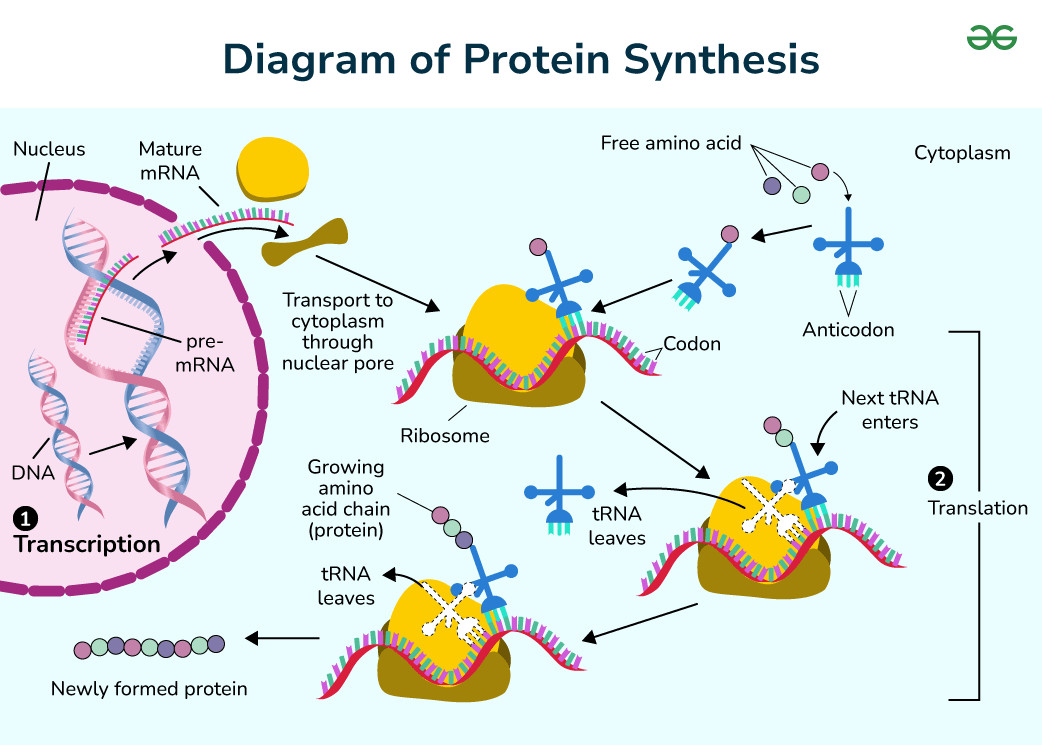
\includegraphics[width=0.9\textwidth]{resources/images/protein_synthesis.png} \\
		\caption{An illustration of the gene translation process in a cell via protein-factories known as ribosomes\cite{geeksforgeeks2024protein}}
		\label{FIG2}
\end{center}
\end{figure}
    
    
In later section (\textbf{\hyperref[SEC4]{Chapter \ref{SEC4}}}) we shall deal with [whole] genome expression, and shall especially deal with hypothetical systems and use the modal sequence concept as the basis for exploring expression and/or manifestation of an entire organism from just its basic genetic code. In this section though, we shall focus on actual expression in real and natural biological systems, and shall focus more on expression at a molecular level --- essentially, at the level of protein manifestation via \textbf{gene expression}.\\


\fbox{\begin{minipage}{0.9\textwidth}
\large

\begin{defn}[The \textbf{DNA and RNA Codon Symbol Sets}, $\psi_{DNA}^*$ and $\psi_{RNA}^*$]
\label{DEFNDNACODONSS}
If $\Theta_n$ is a DNA sequence of length $n$ --- meaning, it contains $n$ nucleotides or $n$ symbols from $\psi_{DNA}$, then, if each triplet of symbols in $\Theta_n$ is replaced by its corresponding 3-gram/CODON, then, we can re-write $\Theta_n$ as a sequence of terms from a special symbol set $\psi_{DNA}^*$:

\begin{equation}
\label{EQSSDNACoDONS}
\psi_{DNA}^* = \langle \alpha_1, \alpha_2, \cdots , \alpha_{64} \rangle
\end{equation}

Such that:

\begin{equation}
\label{EQDNACODCARD}
 \invpi(\psi_{DNA}^*) = \invpi(\psi_{DNA})^3 = 4^3 = 64
\end{equation}

And that each distinct codon has a corresponding standard name associated with either its corresponding amino-acid or whether it is a STOP-codon\cite{gregory1987oxford}\cite{wikipedia_codon_tables}. We shall refer to $\psi_{DNA}^*$ as the \textbf{DNA Codon Symbol Set}.


Further, since RNA sequences are similar to DNA sequences with just the symbols `T' swapped with `U' (see \textbf{\hyperref[DEFRNASS]{Definition \ref{DEFRNASS}}} and \textbf{\hyperref[TRANSF1]{Transformer \ref{TRANSF1}}}), we can also expect that for RNA sequences, there would be an equivalent symbol set for RNA-codons as such:

\begin{equation}
\label{EQSSRNACoDONS}
\psi_{RNA}^* = \langle \beta_1, \beta_2, \cdots , \beta_{64} \rangle
\end{equation}

And the names of the codons in $\psi_{RNA}^*$ are similar to those in $\psi_{DNA}^*$ by the following rule:

\begin{equation}
\label{EQNAMINGRNACodons}
name(\beta_i) = name(\alpha_i) \quad \forall \beta_i \in \psi_{RNA}^*: \beta_i = O_{mRNA-encode}(\alpha_i)
\end{equation}


\end{defn}
\end{minipage}}
\\


It shall be interesting to note that for genetic code in natural automata (nature-like bio-automata\footnote{My research assistant --- thanks \textbf{Microsoft Copilot}, did bring it to my attention that the term ``bio-automata" is ``usually reserved for models or conceptual representations of biological systems --- especially those designed to simulate behaviors, growth patterns, or decisions-making processes using predefined rules, like in cellular automata or agent-based modeling." And thus, much as I often find it attractive to use the term --- as an umbrella term including actual living organisms which, from the perspective of the computer scientist in me, are still correctly classifiable under the "biological automata" category in my opinion since they actually operate on some infallible inherent natural program in their DNA. But, I shall adhere to the advise of my assistant for now.} and generally living things), the most important reason the genetic coding language exists, is so that the body/host-organism system can produce required materials as and when they are needed or demanded for. This for example means producing new or extra body tissue in a still growing organism or in one with any damaged or missing tissue, and essentially, such productions are about the synthesis of particular molecules in the body's system that are basically proteins. The diagram in \textbf{Figure \ref{FIG2}} is a basic illustration of the process for living organisms --- eukaryotes especially.

For simplicity's sake, we can assume the following summarization of the basic process that fully and correctly breaks down the typical ordeal:

First, we shall assume that given the protein is just a chain of amino-acids, we might as well just think of it as though it were an ordered sequence of some terms, and thus, in keeping with the notation from transformatics, we might just refer to such a protein with our usual typical \textbf{resultant sequence} symbol --- $\Theta^*$.

And so, given that these proteins are actually nearly direct/1-to-1 mappings from the corresponding DNA sub-sequence code of a finite length, we might then refer to the DNA sequence that encodes the instructions for producing $\Theta^*$ with just the basic typical transformatics \textbf{source sequence} symbol: $\Theta$ --- more conveniently, because we wish to also talk of the length of the sequence, we might preferably write the DNA sequence code of length \textbf{n} (meaning for example, \textbf{it contains exactly n DNA-codons}), as $\Theta_n$. So, for example we might more fully express $\Theta_n$ as such:

\begin{equation}
\label{EQ1}
\Theta_n = \langle \alpha_{ij}, \rangle ;
\alpha_{ij} \in \psi_{DNA}^* \quad \forall j \in [1,n],  i \in [1,64] \quad \land \quad n \in \mathbb{N}
\end{equation}\\

\textbf{Equation \ref{EQ1}} being just a sometimes preferable way to write the same exact sequence as:
 
 
 \begin{equation}
\label{EQ2}
\Theta_n = \langle a_1,a_2,a_3,...,a_i,...,a_{n-1},a_n \rangle ;
\forall i \quad \exists a_i \in \psi_{DNA}^* \quad \land \quad n \in \mathbb{N}
\end{equation}\\

We have defined the special symbol sets $\psi_{DNA}^*$ in \textbf{\hyperref[DEFNDNACODONSS]{Definition \ref{DEFNDNACODONSS}}} and  $\psi_{DNA}$ in \textbf{Definition \ref{DEFDNASS}}, and as for $\psi_{DNA}^*$, we of course know that it essentially is the set of the distinct 64 codons (see \textbf{Table 1} in \cite{gregory1987oxford}) that \textit{especially} encode amino acids, and which were first introduced in \textbf{\hyperref[SEC1]{Chapter \ref{SEC1}}}. Another way to expound on this is by saying that:

 \begin{equation}
\label{EQ3}
\Theta_n = \{a_i \quad | \quad a_i = \prod\limits_{\rho \in \psi_{DNA}}^3 \rho \quad \land \quad \forall i \in [1,n], n \in \mathbb{N} \quad \land \quad \psi_{DNA} = \langle A, C, G, T \rangle\}
\end{equation}\\

Thus we might encounter a gene such as $\Theta_4$ composed of exactly 4 codons as shown below:

 \begin{equation}
\label{EQ4}
\Theta_4 = \langle \langle A, T, G \rangle, \langle A, A, A \rangle, \langle T, T, A \rangle, \langle T, A, G \rangle \rangle
\end{equation}\\

Which, might also equivalently be expressed as a flattened sequence if the fact that the nucleobases it contains are always read in triplets/3-grams/tuples of 3 at a time. So that we can merely write it as:\\

 \begin{equation}
\label{EQ5}
\Theta_{4 \times 3} = \langle  A, T, G, A, A, A, T, T, A, T, A, G \rangle
\end{equation}\\

So we imply that under the flat-structure notation, the sequence has exactly $4 \times 3$ elements. By this fact and the observation that the previous nested notation merely helps to group together each codon's members within a meaningful sub-sequence, and that the order is otherwise maintained in the flat-sequence structure, we might then also equivalently express the same actual DNA code sequence as an $n \times 3$ matrix as shown below:

 \begin{equation}
\label{EQ5a}
\Theta_{4 \times 3} = \begin{pmatrix}
A& T& G\\
A& A& A\\
T& T& A\\
T& A & G \\
\end{pmatrix}
\end{equation}\\


Whether to actually express it as a $3 \times n$ matrix or as $n \times 3$ might be up to the particular taste of the mathematician or scientist, but otherwise, we know that the ordered sequence $\Theta$ in any of the forms above is essentially a \textbf{genetic program} to guide a DNA code processor such as a ribosome construct a corresponding protein based on the equivalent transcribed mRNA code sequence $\Theta_4^*$ written in mRNA code as such:


 \begin{equation}
\label{EQ6}
\Theta_4^* = \langle \langle A, U, G \rangle, \langle A, A, A \rangle, \langle U, U, A \rangle, \langle U, A, G \rangle \rangle
\end{equation}\\

Which is what we would obtain after a necessary \textbf{DNA} $\rightarrow$ \textbf{mRNA} transform attainable via a DNA sequence transformer we might define as such:\\


\begin{transf}[\textbf{DNA to mRNA Encoder}]
\label{TRANSF1}
$\Theta_n \quad \xrightarrow{O_{mRNA-encode}(\cdot)} \quad \Theta^*_n \quad;$\\
$\forall a_i \in \Theta_n = \langle a_i,\rangle:n, \quad a_i \in \psi_{DNA} \equiv \{A, T, C, G\}$,\\
and if $\exists a_i \in \Theta_n : a_i = T \implies \exists a_i^* \in \Theta^*_n: a_i^* = U$\\
Otherwise $a_i = a_i^* \implies \invpi(a_i = T \in \Theta_n) = \invpi(U \in \Theta^*_n) \quad \land \quad \invpi(\Theta_n) = \invpi(\Theta^*_n) = n$.

\end{transf}

\begin{table}[h]
  \centering
  \Large
	\begin{tabular}[t]{|c|c|c|p{3cm}|}
	\hline
	i & $a_i$ & \textbf{Amino Acid (Code-name)} & \textbf{Function}\\
	\hline
	\hline
	1 & ATG & Methionine (Met) & Start Codon: initiates translation\\
	\hline
	2 & AAA & Lysine (Lys) & Basic amino acid\\
	\hline
	3 & TTA & Leucine (Leu) & Non polar amino acid\\
	\hline
	4 & TAG & Stop (Amber) & Terminates translation\\
	
	\hline
	              
\end{tabular}
 \caption{Amino-Acid Codes and Names in $\Theta_4$, a DNA-encoded gene}
  \label{TAB1}
\end{table}

Thus, though the gene in its DNA form comprised of the ordered sequence of amino-acid codes named as in \textbf{Table \ref{TAB1}}, and yet, the resultant sequence after applying \textbf{Transformer \ref{TRANSF1}} to $\Theta_4$ would be as explained in \textbf{Table \ref{TAB2}}.


\begin{table}[h]
  \centering
  \Large
	\begin{tabular}[t]{|c|c|c|p{3cm}|}
	\hline
	i & $a_i$ & \textbf{Amino Acid (Code-name)} & \textbf{Function}\\
	\hline
	\hline
	1 & AUG & Methionine (Met) & Start Codon: initiates translation\\
	\hline
	2 & AAA & Lysine (Lys) & Basic amino acid\\
	\hline
	3 & UUA & Leucine (Leu) & Non polar amino acid\\
	\hline
	4 & UAG & Stop (Amber) & Terminates translation\\
	
	\hline
	              
\end{tabular}
 \caption{Amino-Acid Codes and Names in $\Theta_4^*$, a mRNA encoded gene}
  \label{TAB2}
\end{table}

So, note that the names (and code-names) of the mRNA encoded codons stay the same as those of their corresponding DNA-encoded codons in both tables --- this is actually generally/conventionally so. But also, note that the functions of the individual codons in either scenario are likewise expressed the same. So, this is is because, when the genetic code is actually being executed (such as in standard protein-synthesis), the processor (the ribosome) merely operates on the mRNA-encoded gene and not directly on the original DNA-encoded code sequences.

Also, important to note, the processor only produces an amino acid (as part of the protein synthesis program), only after having encountered a ``start" instruction, and we know that such instructions are the kind encoded by \textbf{start codons}, of which the most universally utilized START-codon is \textbf{ATG/AUG} known as Methionine, but also other rare-scenario\footnote{They are used less frequently, mostly in prokaryotes and some organelles. When used as START codons, they still recruit the initiator tRNA and translate as \textbf{methionine}, not their usual amino acid\cite{copilot_dna_assistant}} START-codons include the mRNA codes GUG and UUG --- used as such in prokaryotes, and then AUU and AUA, used as such in humans only. 

And then, the processor will stop the protein construction task once it encounters a gene instruction of the ``stop" kind. These are encoded using the \textbf{stop codons}, and these are strictly any one of: TAA/UAA (Ochre), TAG/UAG (Amber) and TGA/UGA (Opal)\cite{newsmedical2025startcodons}.

That said, further note that, after processing the gene, and/or after encountering a stop-codon, the ribosome (also understood as the ``protein factory") is then triggered to detach (from the ``assembly line") and then release/return the final assembled protein thus far. These resultant proteins are basically just a chain of \textbf{actual amino acids} generally starting with the Met-amino acid.

And then, further note that, in case any codons were encountered before the AUG (or rather \textit{start-codon}), these shall then be merely be skipped --- they aren't processed or won't translate into any product such as the usual case of producing an amino-acid (this, even if they would normally have triggered the production of some amino acid). 

\section{Protein Manufacturing Algorithm}
\label{SECPROT}

So, overall, we might sum up this critically important protein generation process with a convenient formalism such as with a protein-production algorithm expressed as in the flow-chart depicted in \textbf{Figure \ref{FIG3}}.


\begin{figure}[H]
  \begin{center}
  %\includegraphics[trim=2cm 8cm 2cm 8cm, clip, width=0.9\textwidth,]{resources/pdfs/ProteinSynthesisStateMachine.pdf}\\
   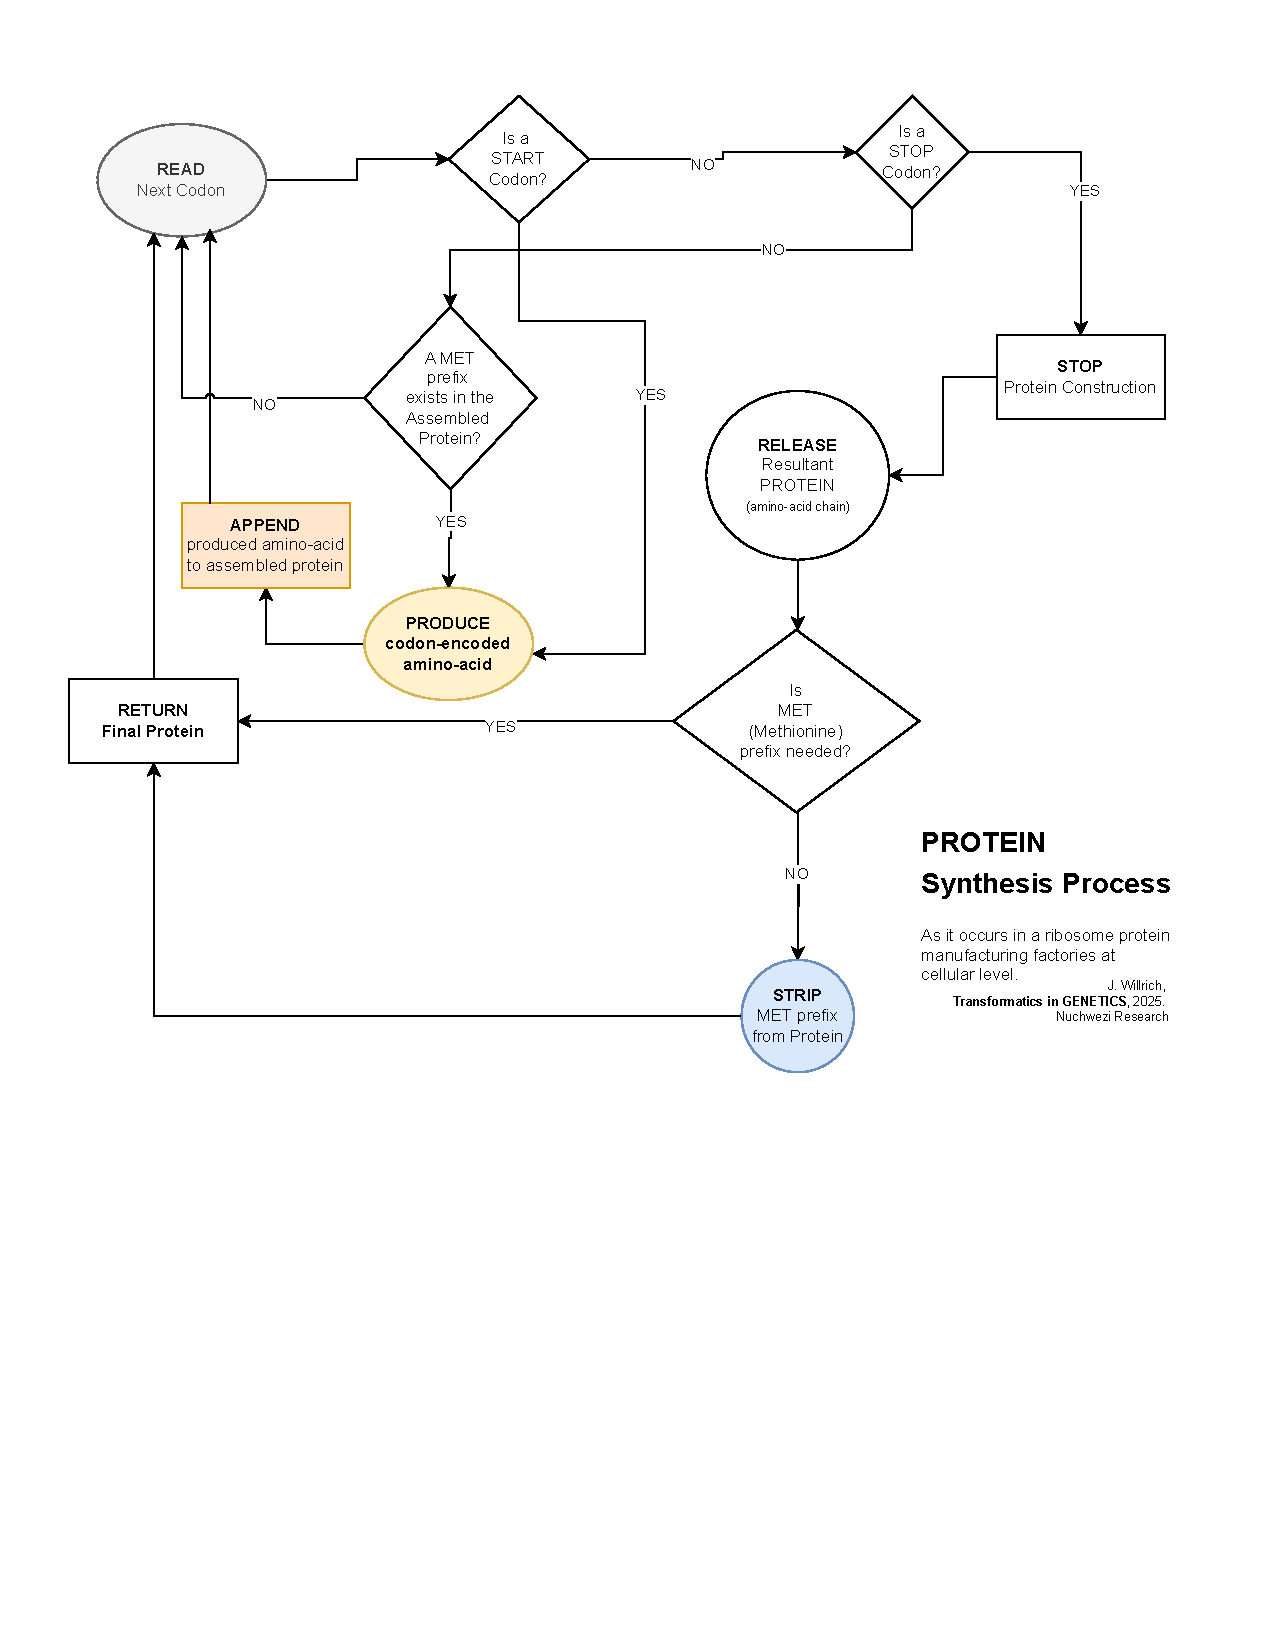
\includegraphics[trim=0cm 8cm 0cm 0cm, clip, width=0.9\textwidth,]{resources/pdfs/ProteinSynthesisProcessFlowChart.pdf}\\
   \caption{\textbf{Flow-Chart summarizing the Ribosome-based Protein-Synthesis Process in a Living Cell}}
  \label{FIG3}
  \end{center}
\end{figure}

That process which is depicted in \textbf{Figure \ref{FIG3}} is how the ribosome protein-manufacturing factory operates at a cellular level as depicted using a \textbf{Flow Chart Diagram} --- meaning, the states of the operating environment as well as those of the operator (the ribosome) are interlaced with decision-making scenarios so as to bring to mind the logic behind how the process proceeds. However, in a different diagram --- the \textbf{Ribosome State Machine} as depicted in \textbf{Figure \ref{FIG4}}, we clearly abstract everything else away and focus on what actually happens from the point-of-view of the gene code sequence processor --- the ribosome. In a way, that state machine not only depicts the various states the ribosome shall be in while operating on incoming gene-code sequences (kind of \textit{requests for solutions/solution-instances/proteins} to problems/specifications/genes) and then how it goes about producing the out-going amino-acid sequences (the proteins). It might even start to feel like the ribosome is a kind of 3D-printer, which, when presented with the specifications of a particular 3D-sequence, knows to process it (translate it) and then produce the required/specified object that is in the context of biological systems we are looking at here, essentially proteins\footnote{Of course, for someone with a background in computer science and who also has interest in designing not just computer programs but also new kinds of computers - abstract machines or not, studying the ribosome from a computing theory and computer architecture perspective --- such as so one appreciates what Instruction Set the ribosome employs; how the ribosome compares to say a Von-Neumann architecture machine; is it Turing Complete or not? How might a pure-text processing languages such as TEA\cite{lutalo2024software} implement a ribosome simulation in say a web-browser environment?\cite{lutalo_tea_web} or that failing, at least allow for the creation of a protein generator or even an entire organism generator as a simulation of how gene code sequences can be translated into sequences of multi-dimension objects?\cite{lutalo2025transformatic} etc.}.


\begin{figure}[H]
  \begin{center}
   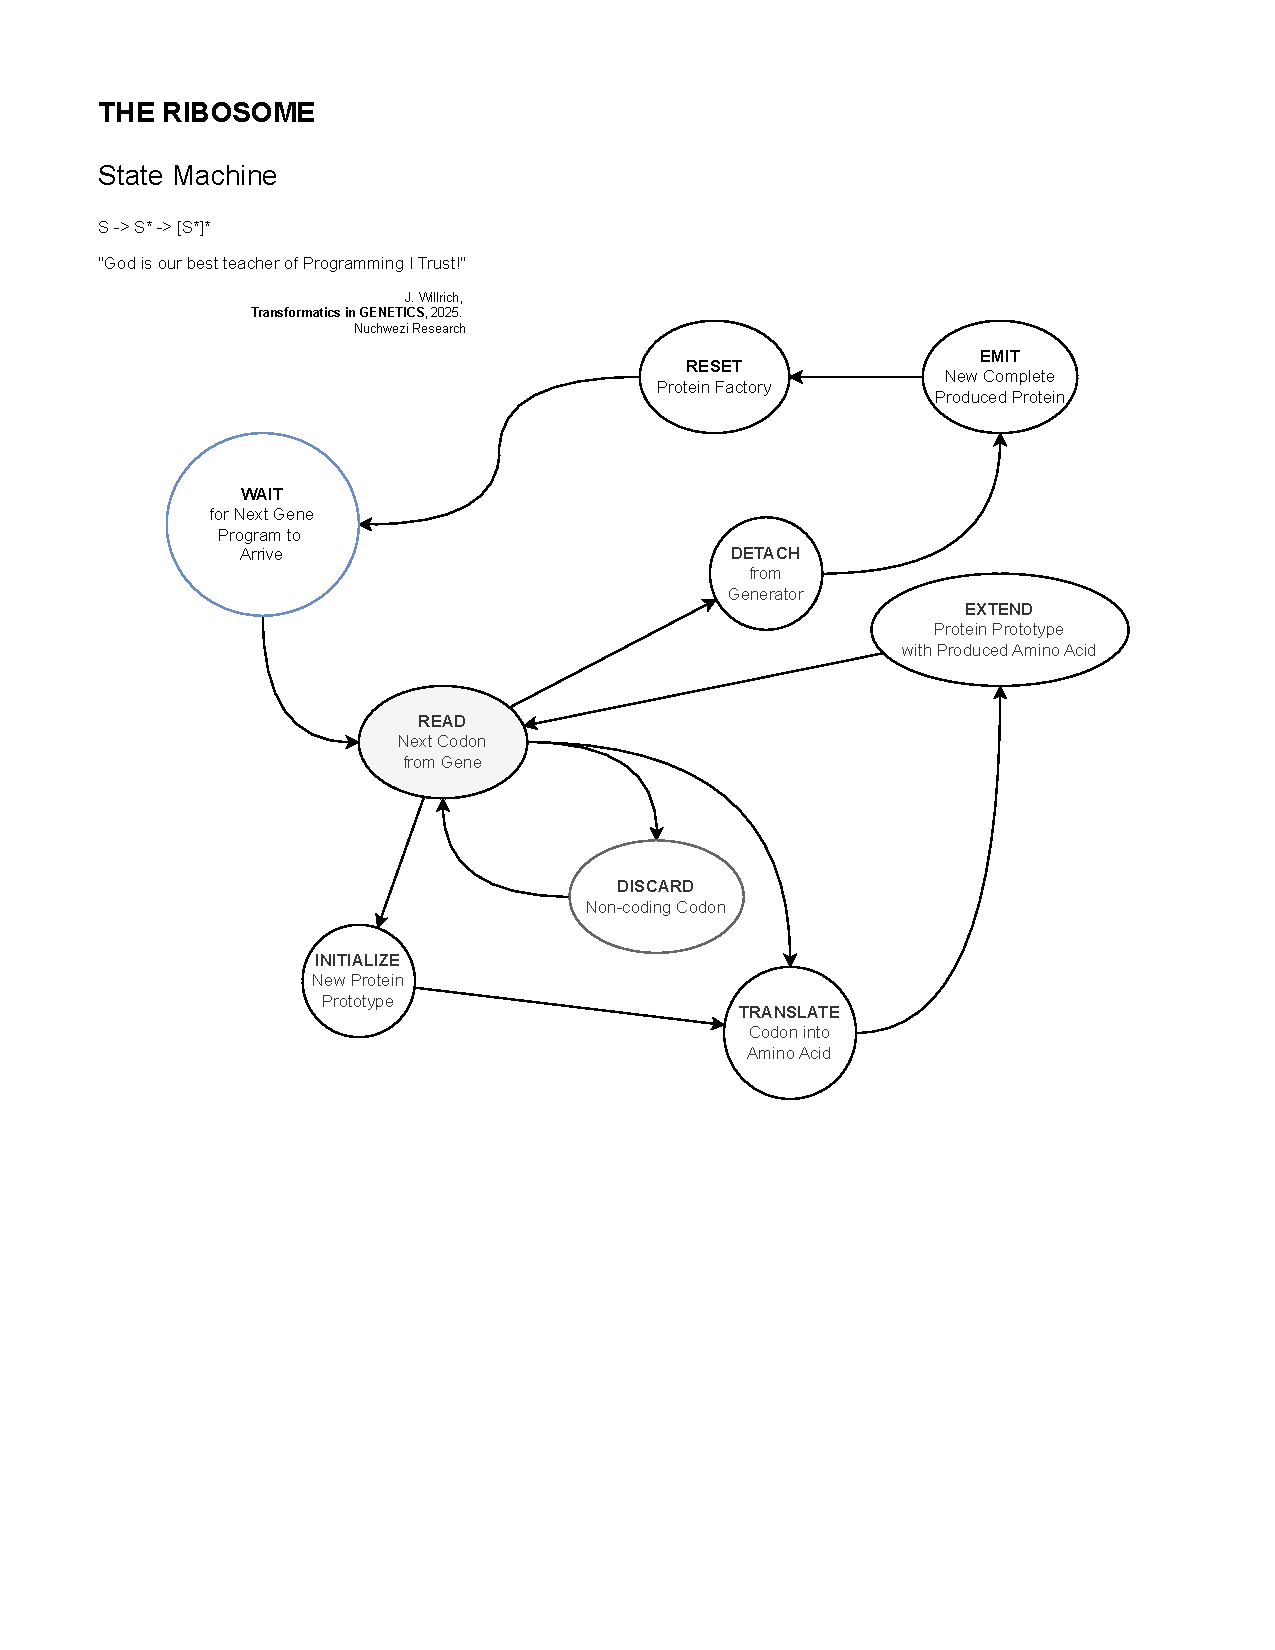
\includegraphics[trim=0cm 9cm 0cm 1.6cm, clip, width=0.9\textwidth,]{resources/pdfs/RibosomeStateMachine.pdf}\\
   \caption{\textbf{The RIBOSOME State Machine}}
  \label{FIG4}
  \end{center}
\end{figure}


Before concluding this section on biological computing systems of the sequence generator kind\cite{lutalo2025transformatic}, it should be worthwhile noting that, as depicted in \textbf{Figure \ref{FIG4}}, the process that is naturally found in every living thing's tiniest cells (excluding viruses as already saw in \textbf{\hyperref[SEC1]{Chapter \ref{SEC1}}}, could be, as with any legitimate state machine, be used to implement a proof-of-concept ribosome processor (or a \textit{ribosome computer} --- a way to implement bio-automatons that behave like a ribosome or which process code similar to DNA and mRNA, or which generally operate on sequences to produce other (possibly more complex) sequences. Thinking of a robotic ribosome might not be something that is immediately required in contemporary medicine or in-organism computing systems, but might be a concept worth adapting or exploring for the design and implementation of self-contained robotic factories for manufacturing and outputting complex products producible via use of a sequence-processing, assembly-line kind of method just as proteins are produced in a bio-cell by the ribosome. We might for example think of ``a sequence from which a finished particular type of car can be manufactured at will" or ``a sequence from which certain kinds of sequence-form/sequence-based\footnote{Vertebrates anyone(?)} artificial and/or organic creatures or bots might be systematically produced at will or on-demand". These kinds of printers --- which, unlike just printers of things on paper, or 3D-printers that know to only produce plastic variants of models they are fed with, but which can say \textit{print a human}\footnote{Though we might touch on it in a future paper on philosophy --- e.g in \textit{Computational Mysticism}\cite{lutalo2024mysticism}, it might be interesting to air-out the author's illuminating view that unlike most other bio-mata such as beasts in the wild or fish in the seas, and definitely not as with silicon-based automatons such as GPT-powered modern \textit{disincarnate} artificial entities --- nor the likes of the ZHA qAGI\cite{jwlzha}, that the human in particular, has this peculiar attribute to them that, apart from just their material substratum as any physical robot might possess or need --- and which is say the domain of ``material producers" such as the ribosome is, and away from their conceptual/software substratum too, they seem to, or perhaps arguably, also possess a preternatural layer of existence that perhaps is or might not have anything to do with their DNA/material-blueprint. A better or more precise classification term for such [\textit{preter-}]intelligent -mata/matter(?) might be the still underground term and concept of a \textit{Psymaton} or \textbf{Psymata} --- bits of this line of discourse have been already touched on in the Psymaz Interview\cite{lutalo2025unraveling}.}, teleport a cow or a banana, etc. might be interesting to explore, as we look into the far-future, where, with humanity's ability to travel and survive in remote and/or unnatural worlds away from their biological home environments (such as Earth's biosphere), might compel them to have to develop new kinds of machines that would not only print out ideas on paper, but also complete food ready-to-eat, medicines to particular kinds of ailments, certain kinds of companion creatures or species, etc. Means to survive on/in alien worlds by leveraging smart, general sequence processors and generators. Talking of which, the next section shall help us start to appreciate this perspective of using the case of genetic code sequences and the ribosome sequence processor into the dimension of both artificial as well as conceptual or hypothetical bio-machines that like the bio-cell can produce complex things via processing of some kinds of code sequences. Bio-automata.

\section{Gene Expression in Living Things and for Bio-Automata via Ribosomes}
\label{SEC5}

One might begin by wondering: \textbf{using the concepts from transformatics and pure mathematics, how might we model or express a general and realistic ribosome?} 

A plausible and meaningful solution to this problem would be to begin by acquiring or developing \textit{a rigorous and correct working definition of what a ribosome is.} The answer would follow directly from that, thus our first definition in this section; a formal definition of a ribosome in any system natural or artificial:


%\fbox{\begin{minipage}{0.9\textwidth}

\begin{defn}[A \textbf{Ribosome}]
\label{DEFRIBOSOME}
Assuming we re-write a sequence of DNA code in terms of the ordered sequence of nucleotides it contains, as in \textbf{Equation \ref{EQ3}} re-written as in \textbf{Equation \ref{EQ7}}:

 \begin{equation}
\label{EQ7}
\Theta_n = \{a_i \quad | \quad a_i = \prod\limits_{\rho \in \psi_{DNA}}^3 \rho \}:n
\end{equation}\\

$\Theta_n$ would then be any sequence of DNA-codons of length $n$, equivalent to an equivalent flat-structure ordered sequence of nucleotides of length $n \times 3$. We can then produce mRNA-codons from $\Theta_n$ as per \textbf{Transformer \ref{TRANSF1}}, so that we produce a new mRNA-codon sequence of length $n$ that is generated as such:

\begin{trans}
\label{TRANS1}
$\Theta_n \quad \xrightarrow{O_{mRNA-encode}(\cdot)} \quad \Theta^*_n;$\\
$\Theta^*_n = \{a_i^* \quad | \quad a_i^* = \prod\limits_{\rho \in \psi_{mRNA}}^3 \rho \}:n$
\end{trans}

And with $\Theta^*_n$ produced, we can then merely generate the corresponding ordered sequence of amino-acids, denoted as $[\Theta^*_n]^*$, via the following mRNA to amino-acid transformer: 

\begin{transf}[\textbf{mRNA to Amino-Acid Translator}]
\label{TRANSF2}
$\Theta^*_n \quad \xrightarrow{O_{mRNA-translate}(\cdot)} \quad [\Theta^*_n]^* \quad;$\\
\begin{enumerate}
\item $\invpi([\Theta^*_n]^*) < \invpi(\Theta^*_n)$ because we only count each codon in the source once, and as per the rules of gene processing/transcription, all non-coding codons (introns) --- basically, codons not able to be translated into an amino-acid given the state of the gene processor\footnote{See \textbf{Figure \ref{FIG3}} and \textbf{Figure \ref{FIG4}}}, don't contribute to the generated resultant sequence in terms of sections it contains --- with the exception of the special ``Met" codon\footnote{A START-codon also counted among genuine ``exons" --- coding codons} that might or might not be retained in the resultant sequence even though it is automatically included as the first produced amino-acid in any legitimate gene sequence.
\item The entire sequence $[\Theta^*_n]^*$ is a kind of 3-Dimension molecule based on the chain of amino-acids it contains, and is technically referred to as a protein.
\end{enumerate}
$\qed$
\end{transf}

A \textbf{Ribosome} then, is any combination of transformers that can result in $[\Theta^*_n]^*$ when presented with just $\Theta_n$ as per the two intermediate transformer processes \textbf{Transformer \ref{TRANSF1}} and \textbf{Transformer \ref{TRANSF2}}, and whose overall processing algorithm is as depicted in \textbf{Figure \ref{FIG3}} and its corresponding state machine as in \textbf{Figure \ref{FIG4}}. 

So, overall, a ribosome is any machine that can implement the combined transformer defined as in \textbf{Transformer \ref{TRANSF3}}:

\begin{transf}[The \textbf{Protein Generator} (A Ribosome)]
\label{TRANSF3}
$\Theta_n  \xrightarrow{O_{mRNA-encode}(\cdot)}  \Theta^*_n  \xrightarrow{O_{mRNA-translate}(\cdot)} [\Theta^*_n]^*;$\\
$\invpi([\Theta^*_n]^*) < \invpi(\Theta^*_n) = \invpi(\Theta_n) = n:$\\
$\psi_{\Theta} = \psi_{DNA} \quad \land \psi_{\Theta^*_n} = \psi_{mRNA} \quad \land \psi([\Theta^*_n]^*) = \psi_{amino-acids}$
\end{transf}

And thus, we can finally merely call any machine capable of implementing the protein generator  in \textbf{Transformer \ref{TRANSF3}} as a \textbf{Ribosome}.

\end{defn}

%\end{minipage}}
%\\

\chapter{Transformatics and Lu-Genome Expression System in Bio-Automata}
\label{SEC4}

\begin{quotation}
\noindent \texttt{Genome Expression: The collective expression profile of all genes within a genome, including coding and non-coding regions, across different conditions, cell types, or developmental stages. It is a systems-level view - measuring how the entire genome behaves dynamically. This includes: mRNA expression of all genes, noncoding RNA activity, epigenetic regulation, chromatin accessibility and transcriptional networks. In essence, gene expression is local, while genome expression is global.}\\
\hspace*{\fill} --- \textbf{Microsoft Copilot}\cite{copilot_dna_assistant}
\end{quotation}

Away from using transformatics to make sense of the differences between organisms based on their genetic code sequences, an even more exciting application of the theory and practical methods of transformatics would be in conceptualizing, analyzing and explaining the important biological, physical, chemical, informational and mathematical concept of \textbf{genome expression}. We shall use a thought experiment and hypothetical cases leveraging exemplary genetic code modeled using special sequences that are treated as modal sequences at minimum.

First, we shall define a basic cipher that can encode the basic digits (of base-10), as some unique, but non-digit forms (essentially, with non-digit \textit{glyphs}). This, so when we speak of a living organism --- for example a pine-apple or a feline, we don't expect that in nature, or rather, that by physically dissecting the organism, that one shall find trapped or stored inside it, the literal genetic code symbols (such as those in $\psi_{na}$), but rather, that they shall find natural literal expressions or instances of genetic code material basis --- such as the chemical base molecules that define nucleobases, or nucleotides, and also complex molecular structures such as transcribed amino-acids post-RNA translation of DNA expressions.

So, in our hypothetical genome expression model --- the \textbf{Lu-Genome Expression System} (LGES), we are going to expect elements from our basic hypothetical DNA symbol set:

\begin{equation}
\label{EQHYPDNASS}
\psi_{\Omega} = \langle 0, 1, 2, 3, 4, 5, 6, 7, 8, 9 \rangle \equiv \psi_{10}
\end{equation}

Which, especially for curiosity's sake, but also, for creative and expressive reasons, is meant to allow us to explore a peculiar genetics model based on not just some four base symbols as is the case in $\psi_{DNA}$, but which allows us to look at any base-10 number expression as a potential genetic code sequence with \textbf{each digit expressing a distinct hypothetical nucleic acid}. For example, we might describe some fictitious organism --- for simplicity's sake, perhaps just a virus that we shall name \textbf{the Euler Virus}\footnote{I called it that, simply because of the fact the associated genome sequence is based on the important natural physical constant --- 2.718281828459, the \textbf{Euler number}, that is one of those irrational numbers that also happens to be the base of the natural logarithm and which arises naturally in many areas of mathematics, especially in calculus, complex analysis, and probability theory.} or just ``veuler", as having its entire genome sequence encoded as just:

\begin{equation}
\label{EQDNAV}
\Omega_{veuler} = 27182818
\end{equation}


However, that is the DNA-side of the story. As in real nature, we need a \textit{different} alphabet or symbol set for expressing genetic code in its \textit{intermediate form} --- as genome expression typically proceeds via expression of DNA into mRNA first of all, and then finally into functions such as proteins. So, in our case, the intermediate expressions shall be expressed using the \textbf{Ozin Cipher}\footnote{More about this in the \textbf{\hyperref[APPOZIN]{Appendix}}.}, which we are to describe hereafter.


\section{The Ozin Genetic Code Cipher}
\label{SECOZIN}

With the background we have obtained thus far, note that the special \textbf{transcription level} expression of our genetic code originally expressed via $\psi_{10}$, shall be transcribed into the intermediate \textbf{ozin genetic code} that spans the symbol set $\psi_{oz}$ that is mapped from the genetic code storage expression via a mapping as depicted in \textbf{Figure \ref{FIGOZIN}}.



\begin{figure}[H]
  \begin{center}
  %\includegraphics[trim=2cm 8cm 2cm 8cm, clip, width=0.9\textwidth,]{resources/pdfs/ProteinSynthesisStateMachine.pdf}\\
   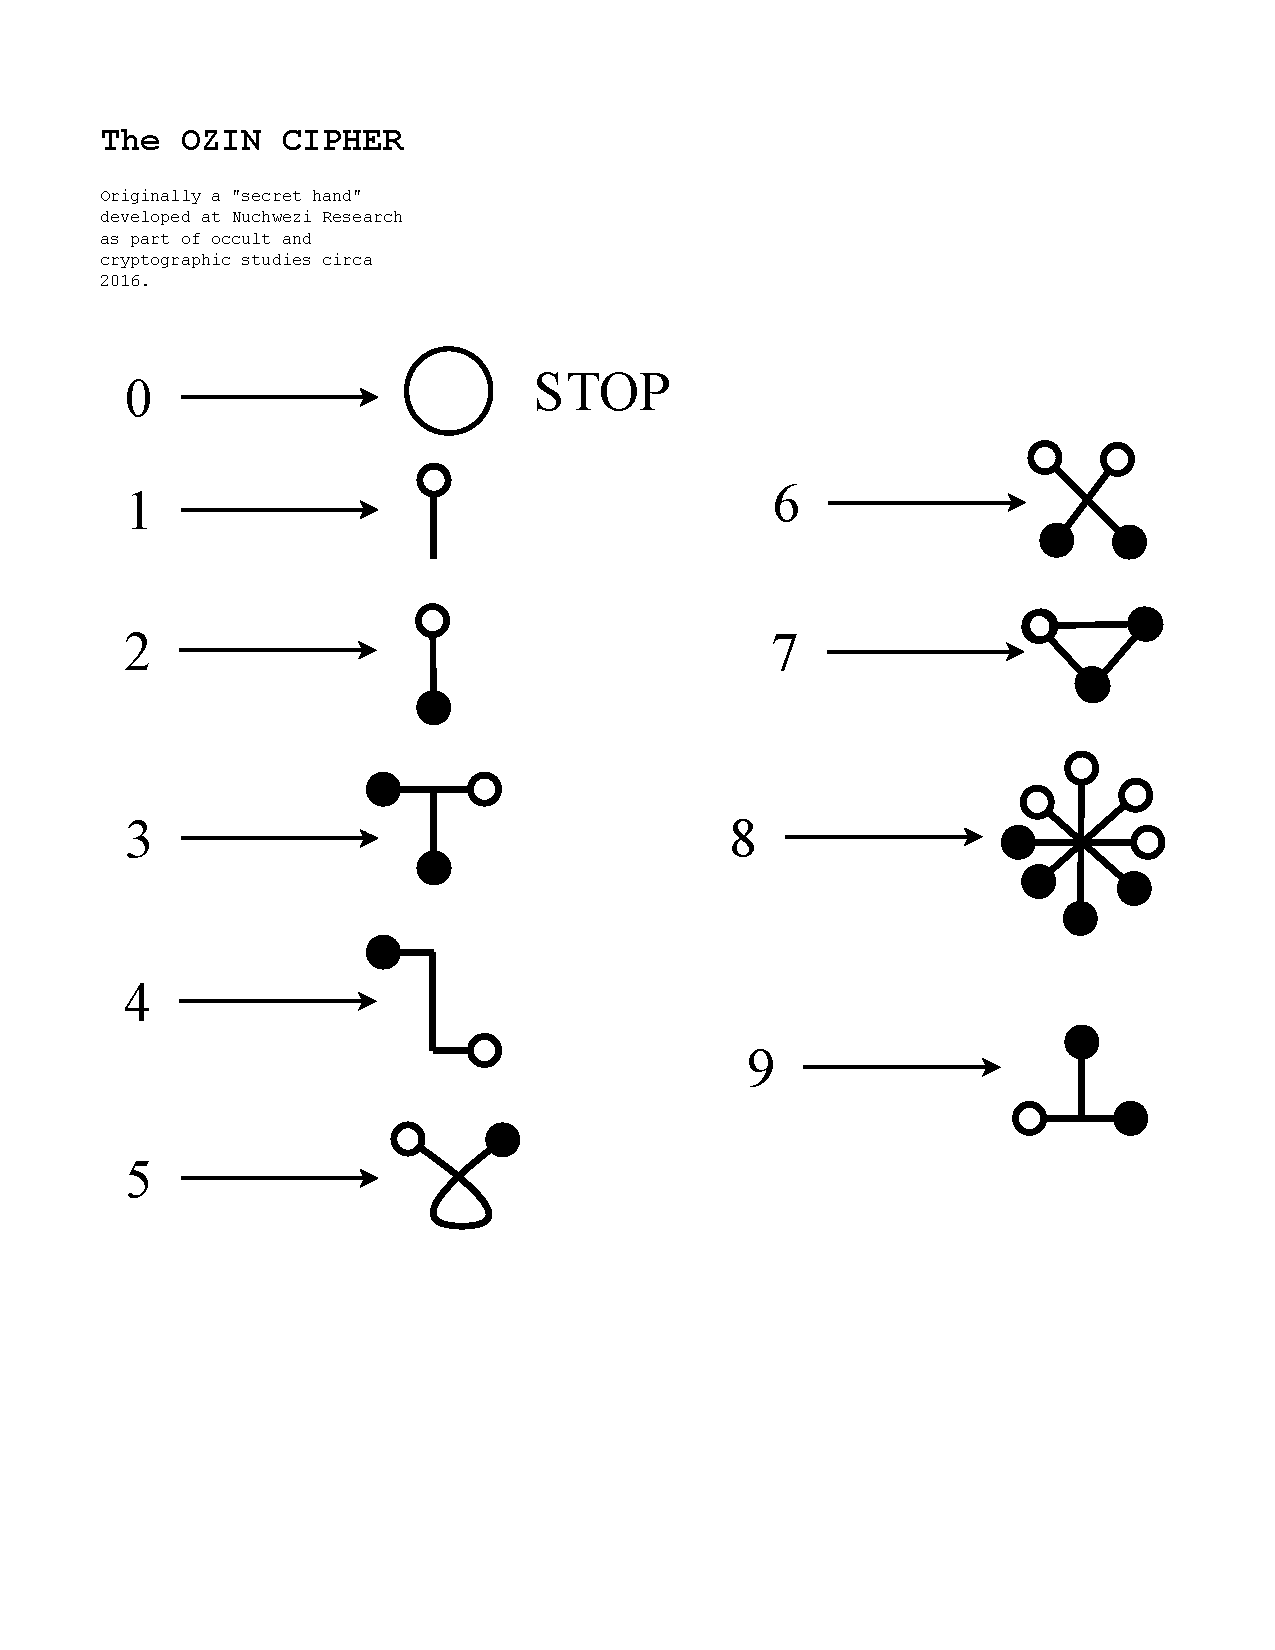
\includegraphics[trim=0cm 6cm 0cm 0cm, clip, width=0.9\textwidth,]{resources/pdfs/OZINCIPHER.pdf}\\
   \caption{The OZIN Cipher\cite{lutalo_2025_ozin}, a mapping from Decimal Symbols (our base-$\Omega$) to Symbols for Intermediate Genetic Code.}
  \label{FIGOZIN}
  \end{center}
\end{figure}


For simplicity's sake, we might interpret or transcribe from base-$\Omega$ DNA into our base-OZ RNA expression as such:

If for some organism such as that expressed via $\Omega_{veuler} = 27182818$, we wish to encode the equivalent intermediate [physical] expression, then we iterate through each symbol in the source code sequence, and re-write it as the equivalent symbolic structure in OZIN, and this, so as to center the ozin glyphs along a \textbf{backbone structure} of just a mere line that starts with a tiny dot and ends with the last ozin structure from the source sequence transcribed. Essentially, for our Euler Virus, it would render as something of the sort shown in \textbf{Figure \ref{FIGOZEVIRUS}}

\begin{figure}[H]
  \begin{center}
  %\includegraphics[trim=2cm 8cm 2cm 8cm, clip, width=0.9\textwidth,]{resources/pdfs/ProteinSynthesisStateMachine.pdf}\\
   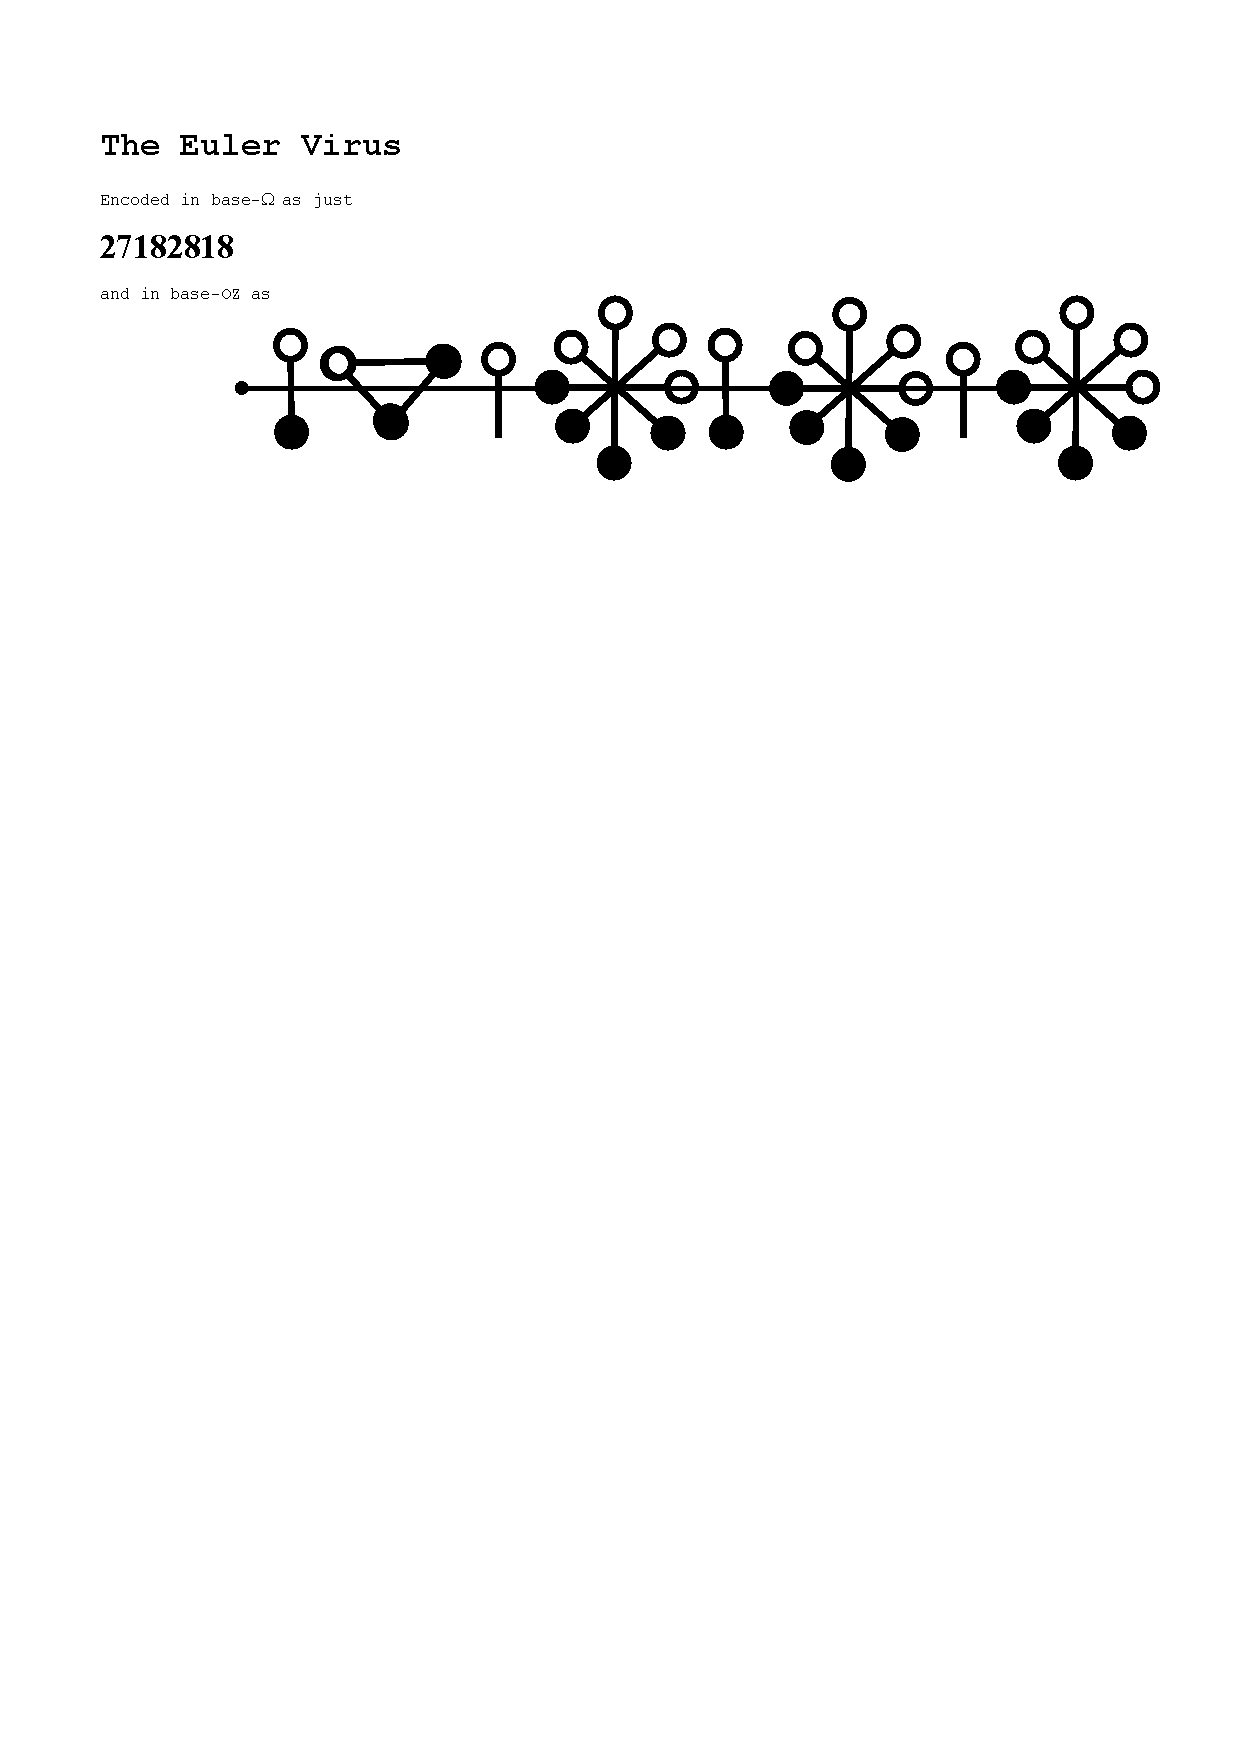
\includegraphics[trim=0cm 20cm 0cm 0cm, clip, width=0.9\textwidth,]{resources/pdfs/OZINCIPHER-APP1-EVIRUS.pdf}\\
   \caption{The equivalent OZIN expression of the hypothetical Euler Virus genome sequence.}
  \label{FIGOZEVIRUS}
  \end{center}
\end{figure}


Another organism, which we might just refer to as the \textbf{HiFinelle}, is actually based off of our favorite base-10 o-SSI --- the \textbf{Hi-Fi o-SSI}\cite{adtpaper}, and thus, its corresponding genetic code at rest is as:


\begin{equation}
\label{EQDNHIFI}
\Omega_{HiFinelle} = 8649137520
\end{equation}


And which, after we have it transcribed into intermediate OZIN genetic expression, shall appear as shown in \textbf{Figure \ref{FIGOZHIFI}}


\begin{figure}[H]
  \begin{center}
  %\includegraphics[trim=2cm 8cm 2cm 8cm, clip, width=0.9\textwidth,]{resources/pdfs/ProteinSynthesisStateMachine.pdf}\\
   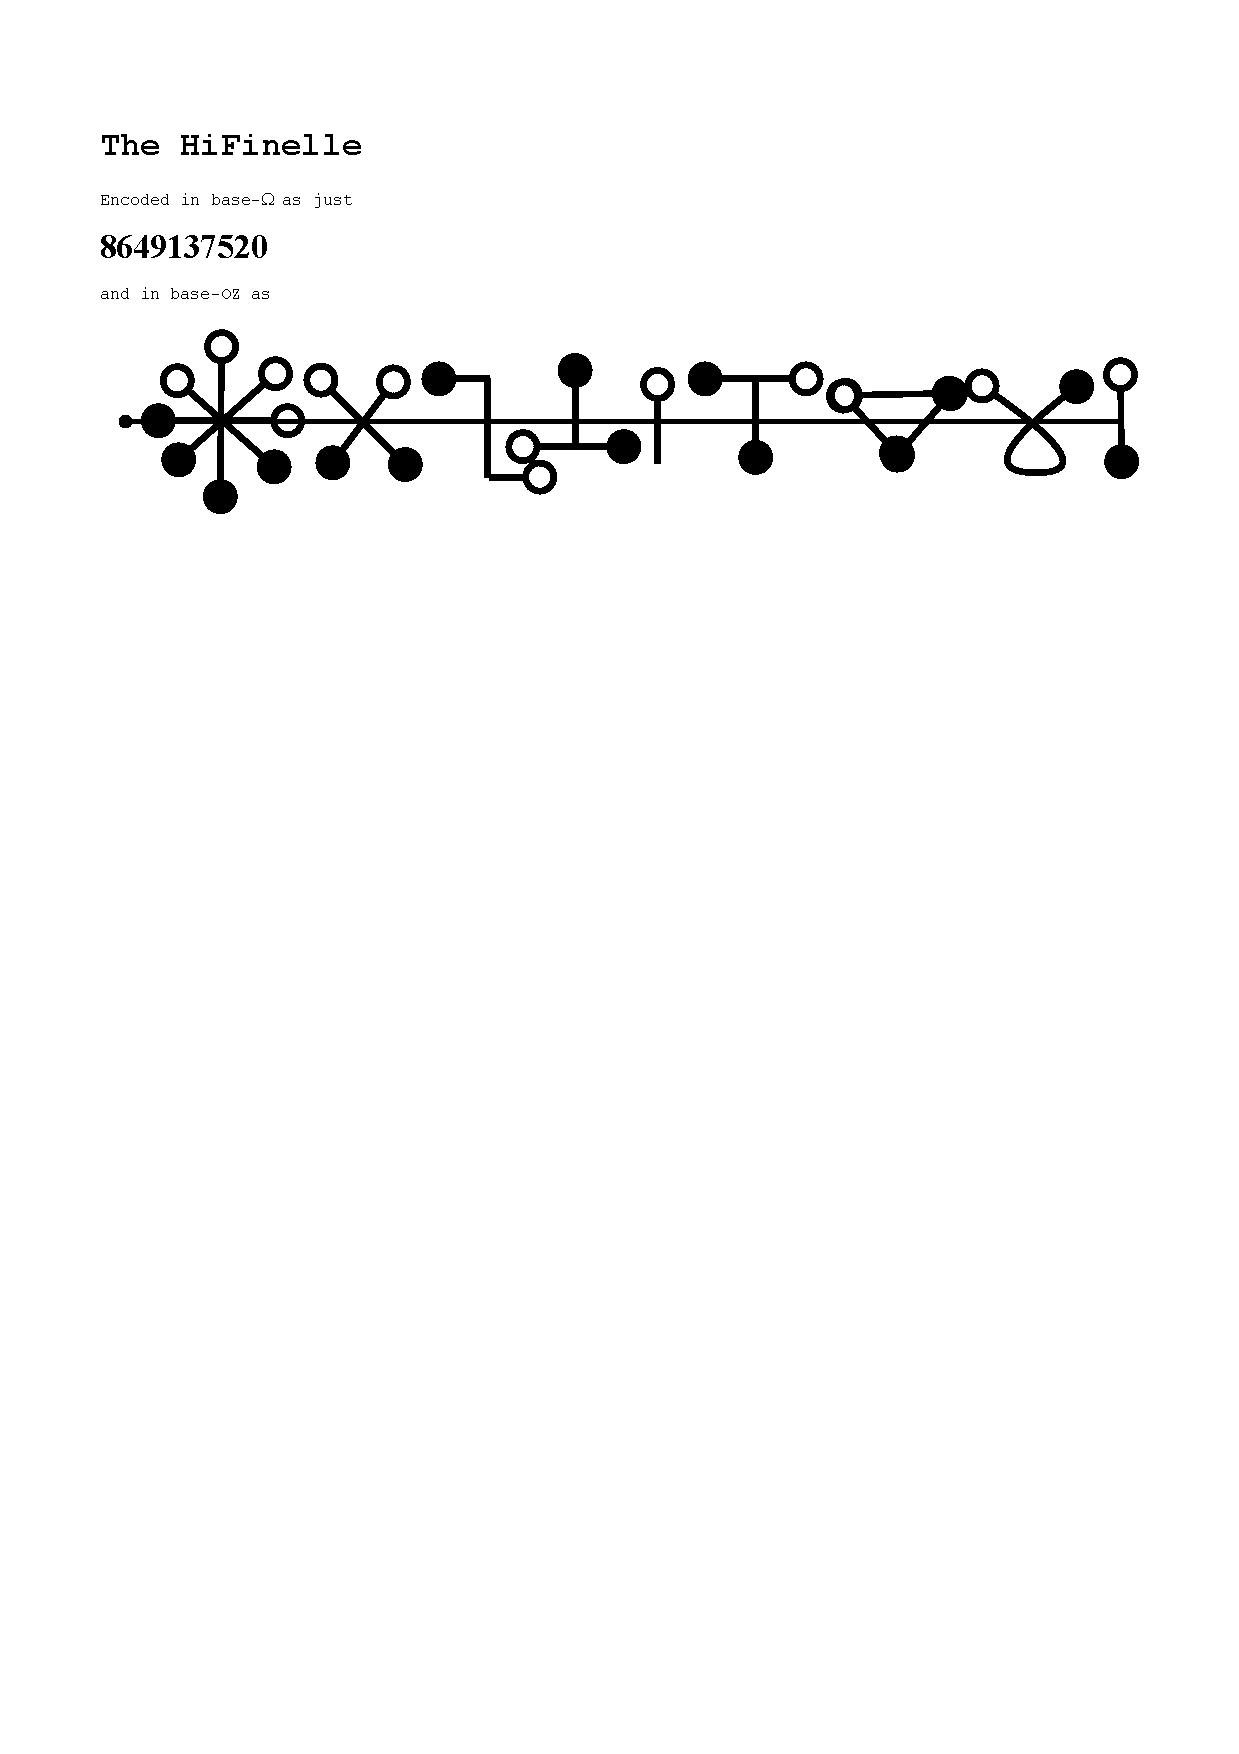
\includegraphics[trim=0cm 20cm 0cm 0cm, clip, width=0.9\textwidth,]{resources/pdfs/OZINCIPHER-APP2-HIFINELLE.pdf}\\
   \caption{The equivalent OZIN expression of the HiFinelle genome sequence.}
  \label{FIGOZHIFI}
  \end{center}
\end{figure}

Of course, in our simplistic genome expression system, the occurrence of that last ``0" symbol in the HiFinelle genome sequence tells us to STOP or just exclude that symbol with a GAP in case any other symbols follow thereafter. It is our STOP-codon equivalent.

Another genome sequence, 

\begin{equation}
\label{EQDNEXA}
\Omega_{3} = 0123026
\end{equation}

Might help illustrate that point --- see \textbf{Figure \ref{FIGOZEXA}}


\begin{figure}[H]
  \begin{center}
  %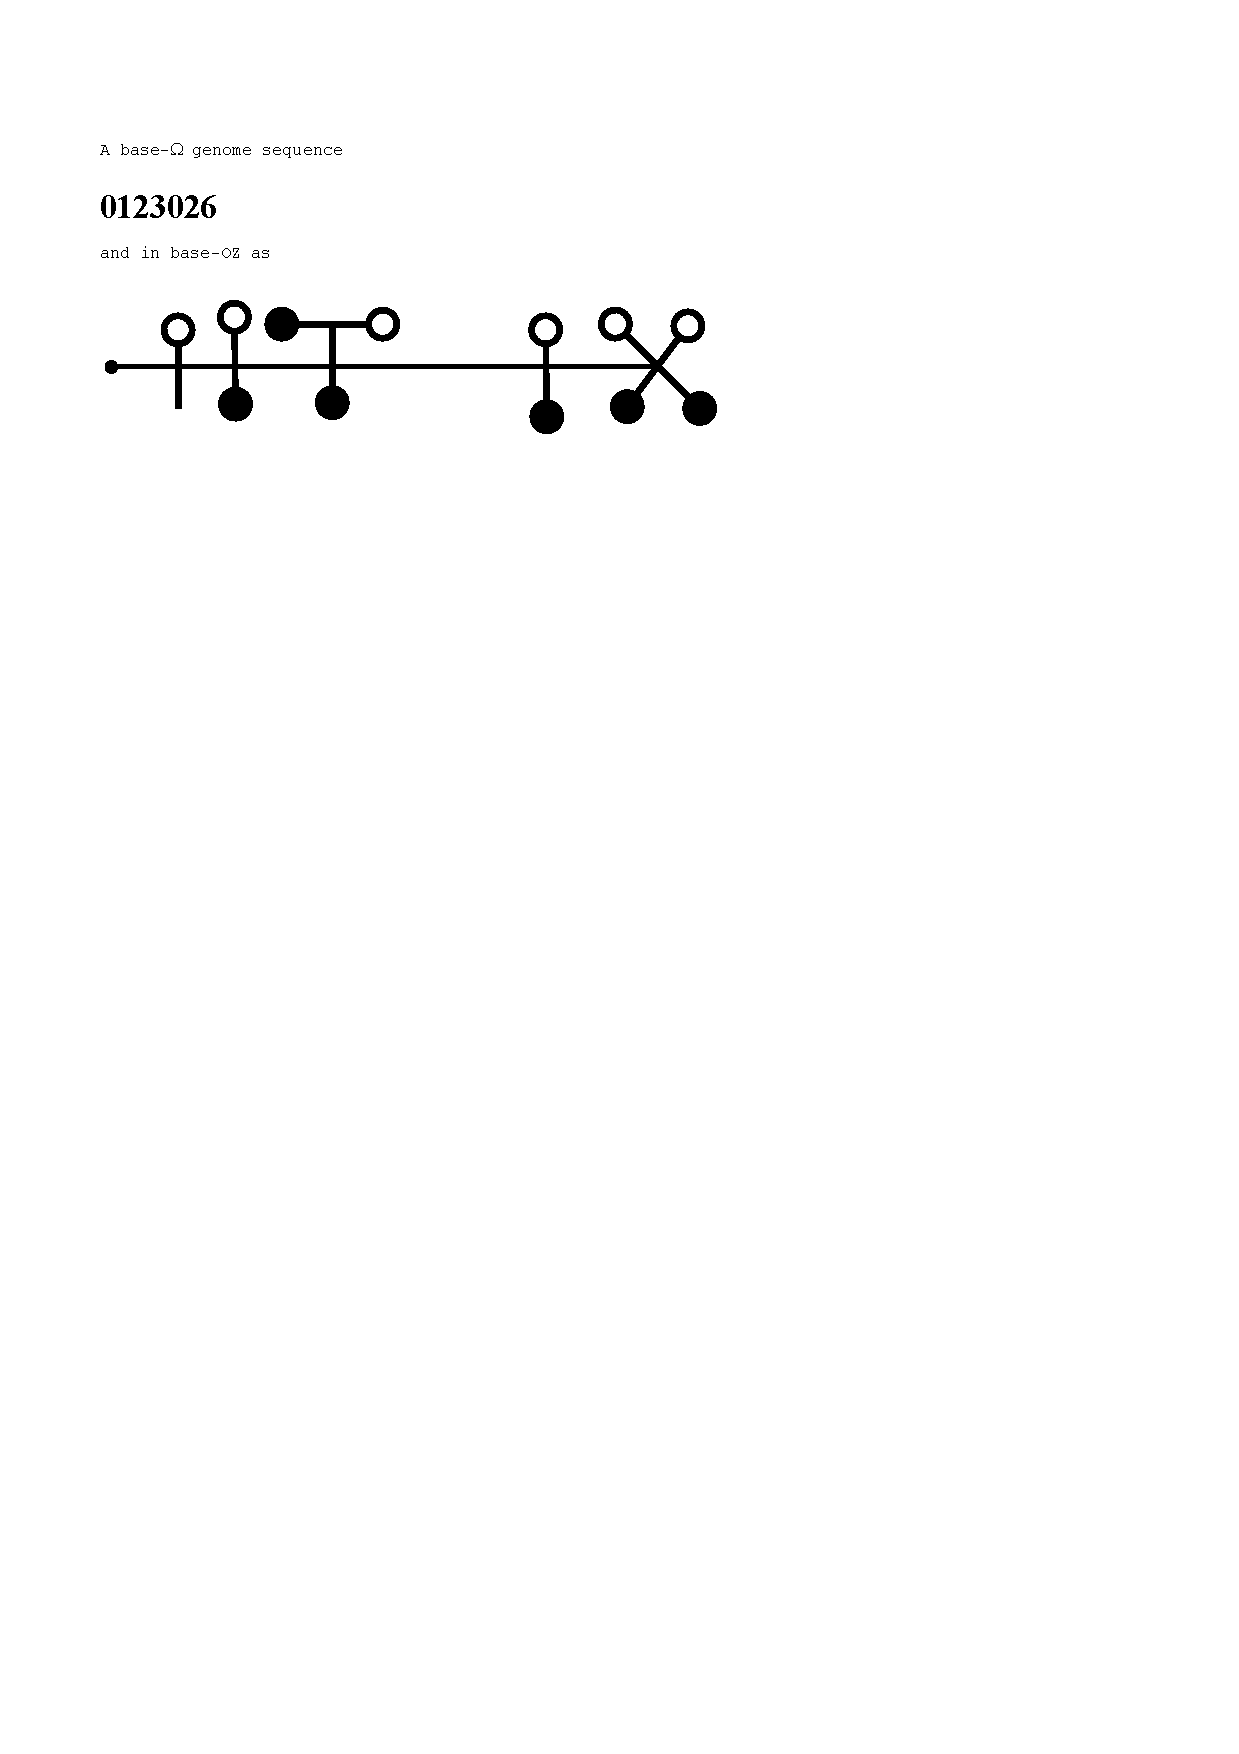
\includegraphics[trim=0cm 20cm 0cm 0cm, clip, width=0.9\textwidth,]{resources/pdfs/OZINCIPHER-APP3-EXA.pdf}\\
   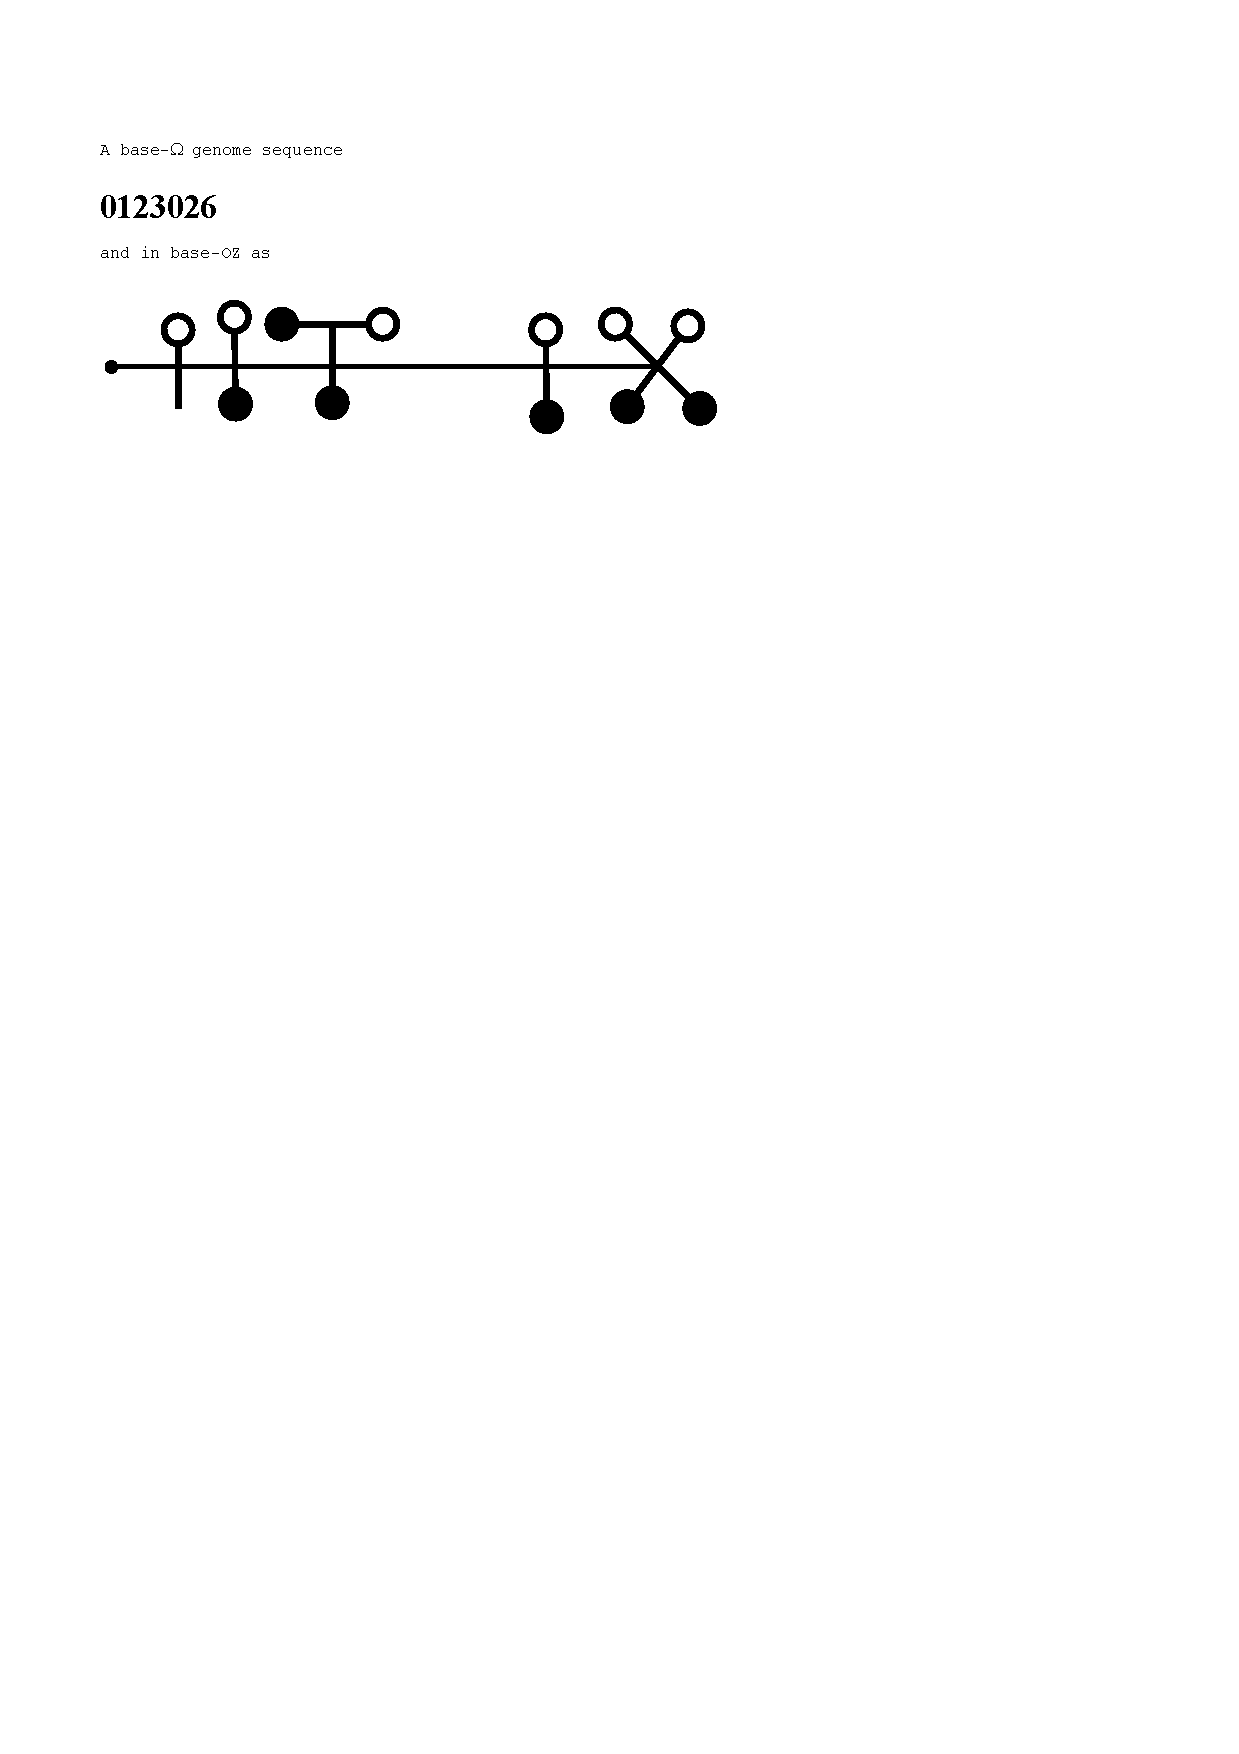
\includegraphics[trim=0cm 22cm 7cm 5cm, clip, width=0.9\textwidth,]{resources/pdfs/OZINCIPHER-APP3-EXA.pdf}\\
   \caption{The equivalent OZIN expression of the $\Omega_{3}$ genome sequence.}
  \label{FIGOZEXA}
  \end{center}
\end{figure}


\subsection{$\Omega$-to-OZIN Genetic Code Transcription Rules}

So, in general, we might sum up our gene transcription rules as such:

\begin{alg}[The \textbf{$\Omega$-to-OZIN Genetic Code Transcription Algorithm}]
\label{ALGCOZIN}

Assuming we have an $\Omega$-base encoded genetic code sequence $\Theta_\Omega$ of some length $n > 0$

\begin{enumerate}
\item Initialize the transcription by constructing a backbone-structure that's essentially just a line with a dot at the head/start. This is the transcribed sequence $OZ(\Theta_\Omega)$.
\item{For each symbol $\omega_i$ in $\Theta_\Omega$: 
\begin{enumerate}
\item Use the transcription mapping: $\psi_\Omega \rightarrow \psi_{oz}$ as depicted in \textbf{Figure \ref{FIGOZIN}}, to encode $\omega_i$  in the equivalent form for the intermediate code.
	\item{If $\omega_i = 0$:
	\begin{enumerate}
	\item{ If $OZ(\Theta_\Omega)$ was still empty:
	\begin{enumerate}
		\item Simply skip to the next symbol in $\Theta_\Omega$ (loop from \textbf{Step\#2)}.
	\end{enumerate}
		}
		\item{ Else: 
		\begin{enumerate}
		\item  Append/Insert a GAP in $OZ(\Theta_\Omega)$
		\item Proceed to the next symbol in $\Theta_\Omega$ (loop from \textbf{Step\#2)}.
		\end{enumerate}
		}
	\end{enumerate}
	}
	\item { Else:
	\begin{enumerate}
	\item Place that encoded version of $\omega_i$ along the backbone structure, $OZ(\Theta_\Omega)$, at the next vacant position ($i$).
	\item Proceed to the next symbol in $\Theta_\Omega$ (loop from \textbf{Step\#2)}.
	\end{enumerate}
	}
\end{enumerate}
}
\item Truncate the backbone-structure after the final term in $OZ(\Theta_\Omega)$.
\item Return $OZ(\Theta_\Omega)$ as the final transcribed version of $\Theta_\Omega$ .
\end{enumerate}

\end{alg}



\subsection{Examples of $\Omega$-Genetic Code Transcription}
\label{SECEXAMTRANSC}

So, now that we have the general transcription rules as in \textbf{Algorithm \ref{ALGCOZIN}}, we can proceed to explore how to leverage them. 

First, note that in \textbf{\hyperref[SEC3A]{Chapter \ref{SEC3A}}}, we have looked at not just the interesting idea of [genetic code] sequence complements, but have also explored several applications of the idea in \textbf{Section \ref{SECAPPCOMPLEMENTS}}, including the concept of the equivalence of sequences under the complement transform. Talking of which, assuming we had a special genome sequence that is made up of subsequences that are complements of each other (such as we might call \textbf{palindromic na-Sequences}) --- e.g $\Theta_{pal}$ defined below, that is actually a palindrome of the two DNA codons --- \textbf{ATG} (Methionine) and \textbf{CAA} (Glutamine) --- the complements being \textbf{GTA} (Valine) and \textbf{AAC} (Asparagine)\cite{wikipedia_codon_tables}.

\begin{equation}
\label{GENOMEPAL}
\Theta_{pal} = \langle A, T, G, C, A, A, A, A, C, G, T, A \rangle
\end{equation}

If we express $\Theta_{pal}$ in our special numeric \textbf{base-$\Omega$}, and then into the visual \textbf{base-OZ}, we shall get something like $\Omega_{pal}$\footnote{Simplified, so we can easily visualize it in base-OZ}:

\begin{equation}
\label{GENOMEPALOMEG}
\Omega_{pal} = \langle 1, 2, 3, 3, 2, 1 \rangle
\end{equation}

And which, if we transcribe it into the intermediate OZIN code, we get:



\begin{figure}[H]
  \begin{center}
  %\includegraphics[trim=2cm 8cm 2cm 8cm, clip, width=0.9\textwidth,]{resources/pdfs/ProteinSynthesisStateMachine.pdf}\\
   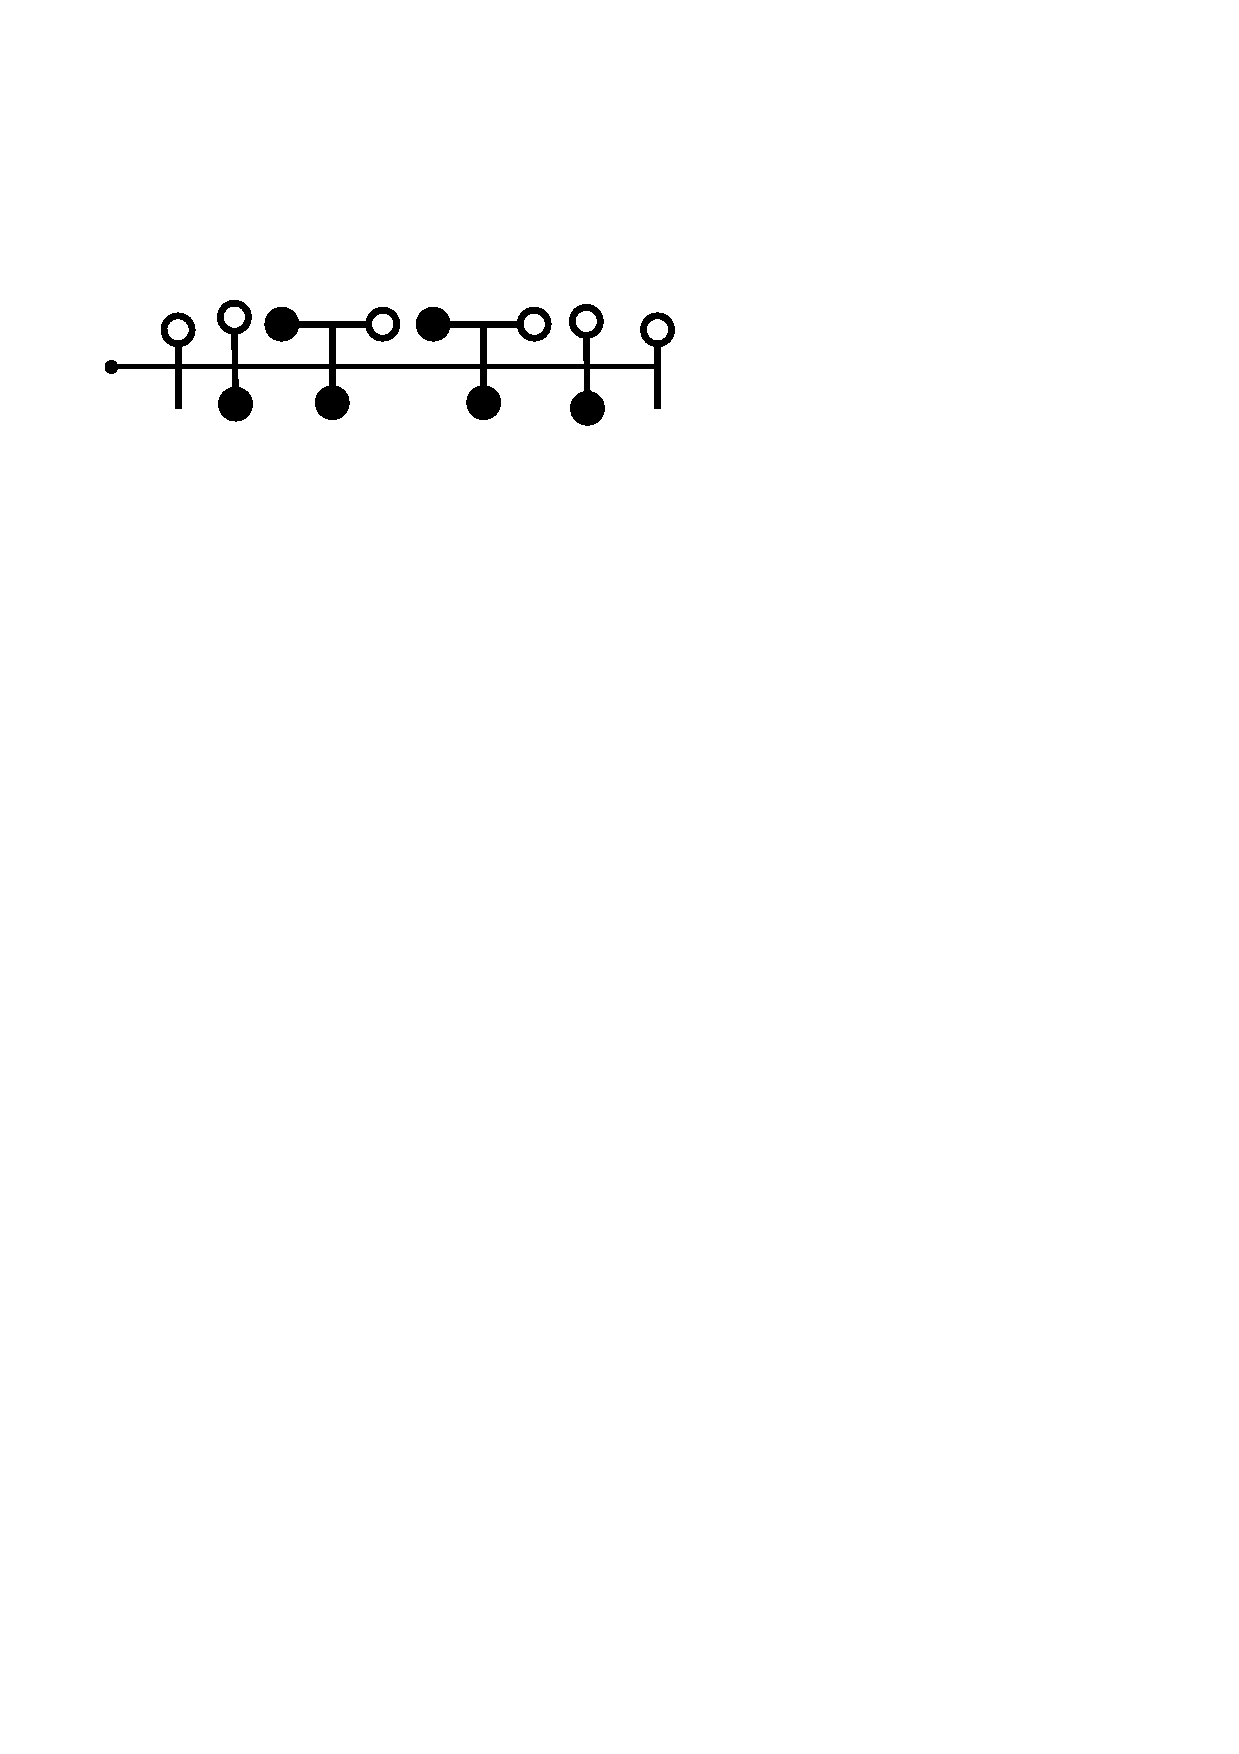
\includegraphics[trim=0cm 22cm 7cm 5cm, clip, width=0.9\textwidth,]{resources/pdfs/OZINCIPHER-APP4-PAL.pdf}\\
   \caption{The palindromic sequence $\Omega_{pal}$ transcribed into base-OZ.}
  \label{FIGOZPAL}
  \end{center}
\end{figure}

Now, notice something interesting here. In particular, if we compare the transcribed forms of $\Omega_{pal}$ and $\Omega_{3}$, we shall notice that even though the two sequences had some differences --- for example, $\Omega_{3}$ contains the ``0" symbol twice, including at the start, and yet, somewhat, because that STOP-codon is skipped during expression/transcription, so we note that the OZIN-expressions of the two sequences are somewhat similar --- they both share a similar prefix structure, that upon inspection of their genetic code sequences, can be attributed to the 3-gram subsequence ``123".

In fact, this later case is an interesting way to appreciate that even where two organisms, genes or proteins might exhibit significant differences in their appearance or even genetic code, and yet, upon close inspection, we might find some telling signs that they share some \textbf{common-traits}. In this case, we see that the palindromic $\Omega_{pal}$ looks somewhat like the otherwise different $\Omega_{3}$ --- at least in their prefix structures after transcription (and possibly beyond!)

\section{Genetic Code Sequences Processed as Modal Sequence Statistics}
\label{SECGENEXPRE}

Now that we have finished looking at how to express genetic code from its base/storage-form (equivalent to DNA) into its intermediate-form (equivalent to RNA), we can then consider the matter of how that intermediate code eventually gets \textbf{translated} into the final organism\footnote{I say ``final organism" here, because, much as in reality, genome expression might be more complex than merely translating genetic code from DNA into RNA and then final proteins and tissue, and yet, conceptually, that is all there is to it!}.

So, in further advancement our thought experiment concerning genome expression (modeled using hypothetical bio-automata), we shall again utilize the OZIN cipher introduced in \textbf{\hyperref[SECOZIN]{Section \ref{SECOZIN}}}, but shall also introduce another formalism in the form of decoding position within a sequence (such as genetic code in this case), as information about how to express or process the associated symbols. This idea, of leveraging \textit{subtle instructions} embedded in genetic code but which might not be explicit as the actual nucleic acid combinations (such as amino-acid encoding-codons), can be justified when we consider that the genetic code processor (such as the ribosome in our major context --- see \textbf{Section \ref{SEC5}}), has a way of interpreting sequences not just by what they contain, but also based on the context within which they exist. For example, though generally the appearance of the RNA codon, \textbf{AAA} would cause the ribosome to synthesize the corresponding amino-acid Lysine (see \textbf{\hyperref[TAB1]{Table \ref{TAB1}}}), and yet, if such a codon appears in a sequence where no earlier instruction compels the ribosome to START manufacturing a protein, the appearance of that codon shall be useless --- or rather, it shall be interpreted differently merely because of being in the wrong context. We saw this in \textbf{Section \ref{SEC05}}, and especially the Ribosome's protein-manufacturing process diagram (\textbf{Figure \ref{FIG3}}) as well as the State Machine (\textbf{Figure \ref{FIG4}}) help bring this out clearly. For example, if we modify the gene-program  in \textbf{Equation \ref{EQ6}} as such:


 \begin{equation}
\label{EQ6B}
\Theta_4^* = \langle \langle A, A, A \rangle, \langle A, U, G \rangle, \langle U, U, A \rangle, \langle U, A, G \rangle \rangle
\end{equation}\\


Then, where we would have expected the ribosome to manufacture protein whose structure includes the AAA/Lysine amino-acid, the result/effect of our modified sequence shall actually be different from what the original gene-program would have produced. In particular, since the START-codon, AUG (Methionine) appears after AAA, the effective protein to be synthesized would be as equivalent to just the program:

 \begin{equation}
\label{EQ6C}
\Theta_4^* = \langle \langle A, U, G \rangle, \langle U, U, A \rangle, \langle U, A, G \rangle \rangle
\end{equation}\\

Which would produce the protein with just \textbf{UUA}(Leucine) in it! So, position of symbols or terms within genetic code matters, and does encode some important gene or even genome expression information that we can't take for granted, thus the following suggested system for how to express post-RNA genetic code sequences.

\subsection{The Platonic Form Cipher and Position-Sensitive Genetic Code Translation}
\label{SECPLATONIC}

Just like we developed a system for how to map numbers (in base-10) to some non-trivial expressions that we equate to a kind of intermediate genetic code (the OZIN-encoded expressions), we shall similarly start by considering a way to map (still base-10) numbers to spatial-structures\footnote{Especially because, and essentially that, when compared to the code that expresses them, proteins and the organism taken as a whole, \textit{occupy more space} than does just the basic DNA code from which they are expressed.}.

So, with the exception of ``0'', which again is treated as an instruction to `skip' or `stop' within our genome expression system\footnote{Perhaps, and as we shall adopt here, we shall interpret `0', especially \textit{within} and not at the start or end of a sequence, to mean not just a GAP as was the case in \textbf{Algorithm\ref{ALGCOZIN}}, but as a JOINT. It somewhat makes biological/anatomical sense.}, we shall adopt the mapping from numbers to spatial-structures as depicted in \textbf{Figure \ref{FIGPLATONICCIPH}} in what we are calling the \textbf{PLATONIC Cipher} System\cite{lutalo_2025_platonic}.


\begin{figure}[H]
  \begin{center}
  %\includegraphics[trim=2cm 8cm 2cm 8cm, clip, width=0.9\textwidth,]{resources/pdfs/ProteinSynthesisStateMachine.pdf}\\
   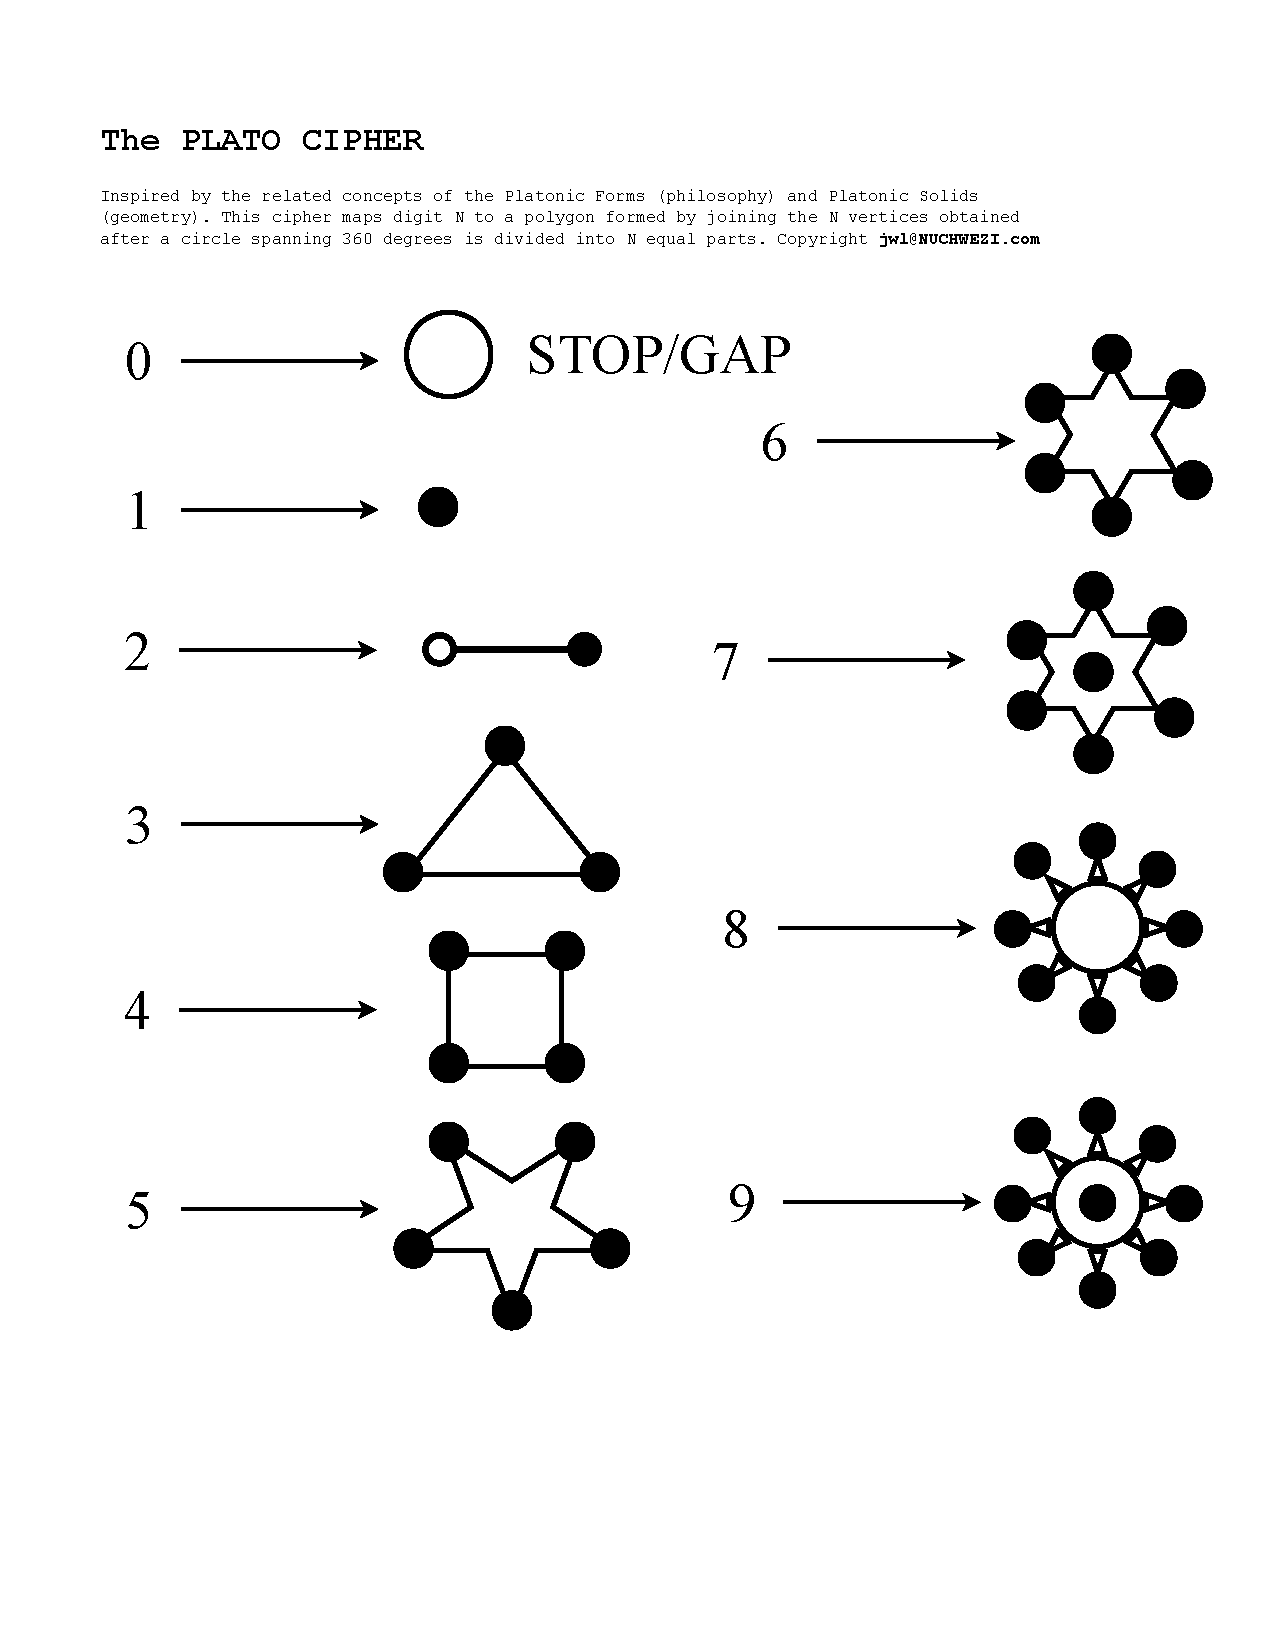
\includegraphics[trim=0cm 4cm 0cm 0cm, clip, width=0.9\textwidth,]{resources/pdfs/PLATOCIPHER.pdf}\\
   \caption{The PLATONIC Cipher\cite{lutalo_2025_platonic} a mapping from Decimal Symbols (our base-$\Omega$) to Spatial-Geometric Forms ($\psi_{pf}$).}
  \label{FIGPLATONICCIPH}
  \end{center}
\end{figure}


How does it work?

\subsection{$\psi_{\Omega}$-to-$\psi_{pf}$: PLATONIC Form Genetic Code Translation Rules}
\label{SECGENSEQEXPRES}


So, in general, we might sum up our start to finish gene (and/or genome) expression with the post-transcription rules and process as such:

\begin{alg}[The \textbf{$\Omega$-to-PLATONIC Form Genetic Code Expression Algorithm}]
\label{ALGCOZINPLATO}

Assuming we have an $\Omega$-base encoded genetic code sequence $\Theta_\Omega$ of some length $n > 0$.

\begin{enumerate}
\item{Initialize the expression with a transcription, by Using \textbf{Algorithm \ref{ALGCOZIN}} to construct the \textbf{Intermediate Form Affix} (IFA) of $\Theta_\Omega$ --- essentially return $OZ(\Theta_\Omega)$ as the start of the \textbf{Final Genome Expression} (FGE) $\boxed{OZ(\Theta_\Omega)}^*$ --- so that the final complete expressed(transcribed+translated ) sequence shall be as:\\

\begin{equation}
\label{EQTRANSLGENSEQ}
\boxed{OZ(\Theta_\Omega)}^* = OZ(\Theta_\Omega)\cdot\boxed{OZ(\Theta_\Omega)}
\end{equation}\\

$\boxed{OZ(\Theta_\Omega)}: \mathbb{N} \times \psi_{pf}$ is the suffix of expressed na-Sequence $\Theta_\Omega$, and is expressed in our genome expression system, as PLATONIC-Form encoded \textbf{modal sequence statistic} of $OZ(\Theta_\Omega)$\footnote{We render the \textbf{suffix of FGE} as $\overset{>}{OZ(\Theta_\Omega)}$ because it allows us to not express $\Theta_\Omega$ naively at the genome or gene level, but also, so that, from an information-theoretic perspective, the completed genome expression is somewhat a statistical summary of what the genome sequence contains --- the appearance of an animal or a plant or virus, depicting or expressing the summary of its DNA code. We do this then, by not merely doing a 1-to-1 translation of the intermediate Ozin-code expression $OZ(\Theta_\Omega)$, but instead computing its summary in form of $\overset{>}{OZ(\Theta_\Omega)}$, and then instead translating that into the final spatial/geometric forms as per $\psi_{pf}$. This is shall complete the entire processing/synthesis of sequence $\Theta_\Omega$, or rather our genome expression.} --- the \textbf{PFA}\footnote{Platonic Form Aspect}, i.e.:\\

\begin{equation}
 \boxed{OZ(\Theta_\Omega)} = \boxed{\overset{>}{OZ(\Theta_\Omega)}}_{pf}
\end{equation}\\


}
\item{ So once we have the \textbf{IFA}, $OZ(\Theta_\Omega)$, proceed to use it to generate the rest of the sequence expression as follows: 
\begin{enumerate}
\item {\textbf{INITIALIZE} FGE, $\boxed{OZ(\Theta_\Omega)}^*$ as just:\\

\begin{equation}
\label{EQSTARTFGE}
\boxed{OZ(\Theta_\Omega)}^* = \langle \langle OZ(\Theta_\Omega) \rangle \langle \rangle \rangle
\end{equation}\\

This ensures, we have the prefix affix, \textbf{IFA}, as the contents of the sequence start of \textbf{FGE} \textit{extended} by a \textbf{still empty subsequence} --- in expression form, this shall merely be a backbone structure with \textbf{IFA} as its head, and a terminal that is ready to have more units appended to it, \textbf{after a single GAP/JOINT extension to IFA}. So, it also means, at this juncture, \textbf{PFA} is just:\\

\begin{equation}
\label{EQSTARTFGESUF}
\boxed{OZ(\Theta_\Omega)} = \langle \rangle
\end{equation}\\

}
\item {
	\textbf{COMPUTE} the \textbf{IFA MSS}, $\overset{>}{OZ(\Theta_\Omega)}$
}
\item {
	\textbf{COMPUTE} $m$, the cardinality of the \textbf{IFA MSS}, $m = \invpi(\overset{>}{OZ(\Theta_\Omega)})$
}
\item {
	\textbf{COMPUTE} the \textbf{Platonic Form Encoding Key}(PFEK), $\boxed{\psi_{pf}}_m$, corresponding to $m$ and based on the \textbf{SLSA Algorithm}\footnote{The \textbf{SLSA}, \textbf{Second Lu-Shuffle Algorithm} is well introduced and explained in \textbf{\hyperref[APPSLSA]{Section \ref{APPSLSA}}}, and it basically is about generating an exact anagram of the input sequence, corresponding to a particular partitioning index --- in this case (and by \textbf{LGES} convention, denoted), $m$, the size of the \textbf{IFA MSS}}
}
\item{\textbf{FOREACH} symbol/term $\omega_i^*$ in \textbf{IFA MSS}, $\overset{>}{OZ(\Theta_\Omega)}$: 
\begin{enumerate}
\item{\textbf{USE} the \textbf{symbol set translation mapping}: $\psi_\Omega \rightarrow \boxed{\psi_{pf}}_m \rightarrow \psi_{pf}$ where that final term corresponds to the mapping depicted in \textbf{Figure \ref{FIGPLATONICCIPH}}, to translate $\omega_i^*$ into the equivalent \textbf{Platonic Form}, $\boxed{\omega_i^*}$, for the final expression as such:}
\item { \textbf{IF} $\omega_i^* \equiv 0$:Operating on the current \textbf{FGE}: 
		\begin{enumerate}
		\item { Append/Insert a JOINT onto \textbf{FGE},  $\boxed{OZ(\Theta_\Omega)}^*$\\

		\begin{equation}
		\label{EQEXTFGEJOINT}
		\boxed{OZ(\Theta_\Omega)}^* = \boxed{OZ(\Theta_\Omega)}^* \cdot \boxed{\omega_i^*}_{joint}
		\end{equation}\\		
		
		And equivalently/thus:\\
		
		\begin{equation}
		\label{EQEXTFGEJOINTSUF}
		\boxed{OZ(\Theta_\Omega)} = \boxed{OZ(\Theta_\Omega)} \cdot \boxed{\omega_i^*}_{joint}
		\end{equation}\\				
		
		}
		\item \textbf{PROCEED} to the next symbol in \textbf{IFA MSS}, $\overset{>}{OZ(\Theta_\Omega)}$\\ (loop from \textbf{Step\#2(e))}.
		\end{enumerate}
	}
	\item { \textbf{ELSE}: \textbf{RESOLVE} the correct  $\boxed{\omega_i^*}$  for  $\omega_i^*$  by using the relation\footnote{Concerning how to actually arrive at the correct $\boxed{\omega_i^*}$ via the correct $\boxed{\psi_\Omega}_m$ for a given \textbf{IFA MSS}, refer to \textbf{\hyperref[SECIFAMSSPFMAPS]{Appendix \ref{SECIFAMSSPFMAPS}}} that covers how to compute or look-up the necessary \textbf{platonic form encoding key}.}\\


\fbox{
\begin{minipage}{0.9\textwidth}

\begin{equation}
\label{EQFBOXED}
 \boxed{\omega_i^*} = \rho_j \in \psi_{pl} +  j \times \omega_i^* : j = \boxed{j} : I(\boxed{j},\boxed{\psi_{pf}}_m) = I(\omega_i^*,\overset{>}{OZ(\Theta_\Omega)})
\end{equation}\\

\end{minipage}}
\\



	\begin{enumerate}
	\item{\textbf{PLACE} that encoded version, $\boxed{\omega_i^*}$, along the existing \textbf{FGE} structure at the next vacant position ($\invpi(\Theta_\Omega)+i$). Expressible with another version of \textbf{Equation \ref{EQEXTFGEJOINT}} as:\\
	
	\begin{equation}
	\label{EQEXTFGEPF}
		\boxed{OZ(\Theta_\Omega)}^* = \boxed{OZ(\Theta_\Omega)}^* \cdot \boxed{\omega_i^*}
		\end{equation}\\
		
		And equivalently:\\
		
		\begin{equation}
		\label{EQEXTFGEPFSUF}
		\boxed{OZ(\Theta_\Omega)} = \boxed{OZ(\Theta_\Omega)} \cdot \boxed{\omega_i^*}
		\end{equation}\\
		
	Where the special \textbf{PFA} term, $\boxed{\omega_i^*}$, as per \textbf{Equation \ref{EQFBOXED}}, is basically the PLATONIC Form corresponding to position $j$ in $\boxed{\psi_{pf}}_m$ --- an \textbf{anagrammatized $pf$-symbol set} relative to $m$ and which is used to look-up the \textbf{correct indices} for the \textbf{corresponding} geometric structure components from $\psi_{pf}$ the symbol set of the final form of the \textbf{PFA}, but also with the \textit{twist} that the intermediate form $\omega_i^*$ is attached to that geometric structure $j$ times --- as depicted in example\footnote{It shall be interesting to note, that based on the \textbf{PFEK} by \textbf{SLSA} --- see \textbf{\hyperref[TABSSLAPERK]{Table \ref{TABSSLAPERK}}}, that assuming we had [an actually \textit{strange}] organism whose equivalent $\Omega$-encoded DNA sequence were just the sequence $\Theta$ = \textbf{666}, its corresponding \textbf{IFA} characteristic would be just $\hbar(\overset{>}{\Theta}) = $\textit{\textbf{6}3}, the corresponding \textbf{MSS} just $\langle$\textbf{6}$\rangle$, and so its \textbf{PFEK} look-up key, $m = \invpi(\overset{>}{\Theta}) = 1$, so that, its corresponding $\boxed{\psi_{pf}}_1 = \langle 4 \rangle$, and so that for its \textbf{BODY} component in the associated full genome expression, the entire \textbf{PFA} would just be $\boxed{\omega_1^*} \implies 4_{pf} \otimes 6_{oz}$ --- which is exactly what we see in this picture in \textbf{\hyperref[FIGEXAPLATONICFORMPFA]{Figure \ref{FIGEXAPLATONICFORMPFA}}}!} \textbf{Figure \ref{FIGEXAPLATONICFORMPFA}}, with each expression of $\omega_i^*$ attached to one of the $j$ \textbf{appendage spots} on the shape for $\boxed{\omega_i^*}$.
	}
	\item \textbf{PROCEED} to the next symbol in \textbf{IFA MSS}, $\overset{>}{OZ(\Theta_\Omega)}$\\ (loop from \textbf{Step\#2(e))}.
	\end{enumerate}
	}
\end{enumerate}
}
\end{enumerate}
}

\item \textbf{TRUNCATE} the final-structure after the final term in \textbf{FGE}.
\item \textbf{RETURN} \textbf{FGE}, $\boxed{OZ(\Theta_\Omega)}^*$ as the final transcribed and translated version of $\Theta_\Omega$. The culmination of our conceptual genome expression.
\end{enumerate}
$\qed$
\end{alg}


\begin{figure}[H]
  \begin{center}
   %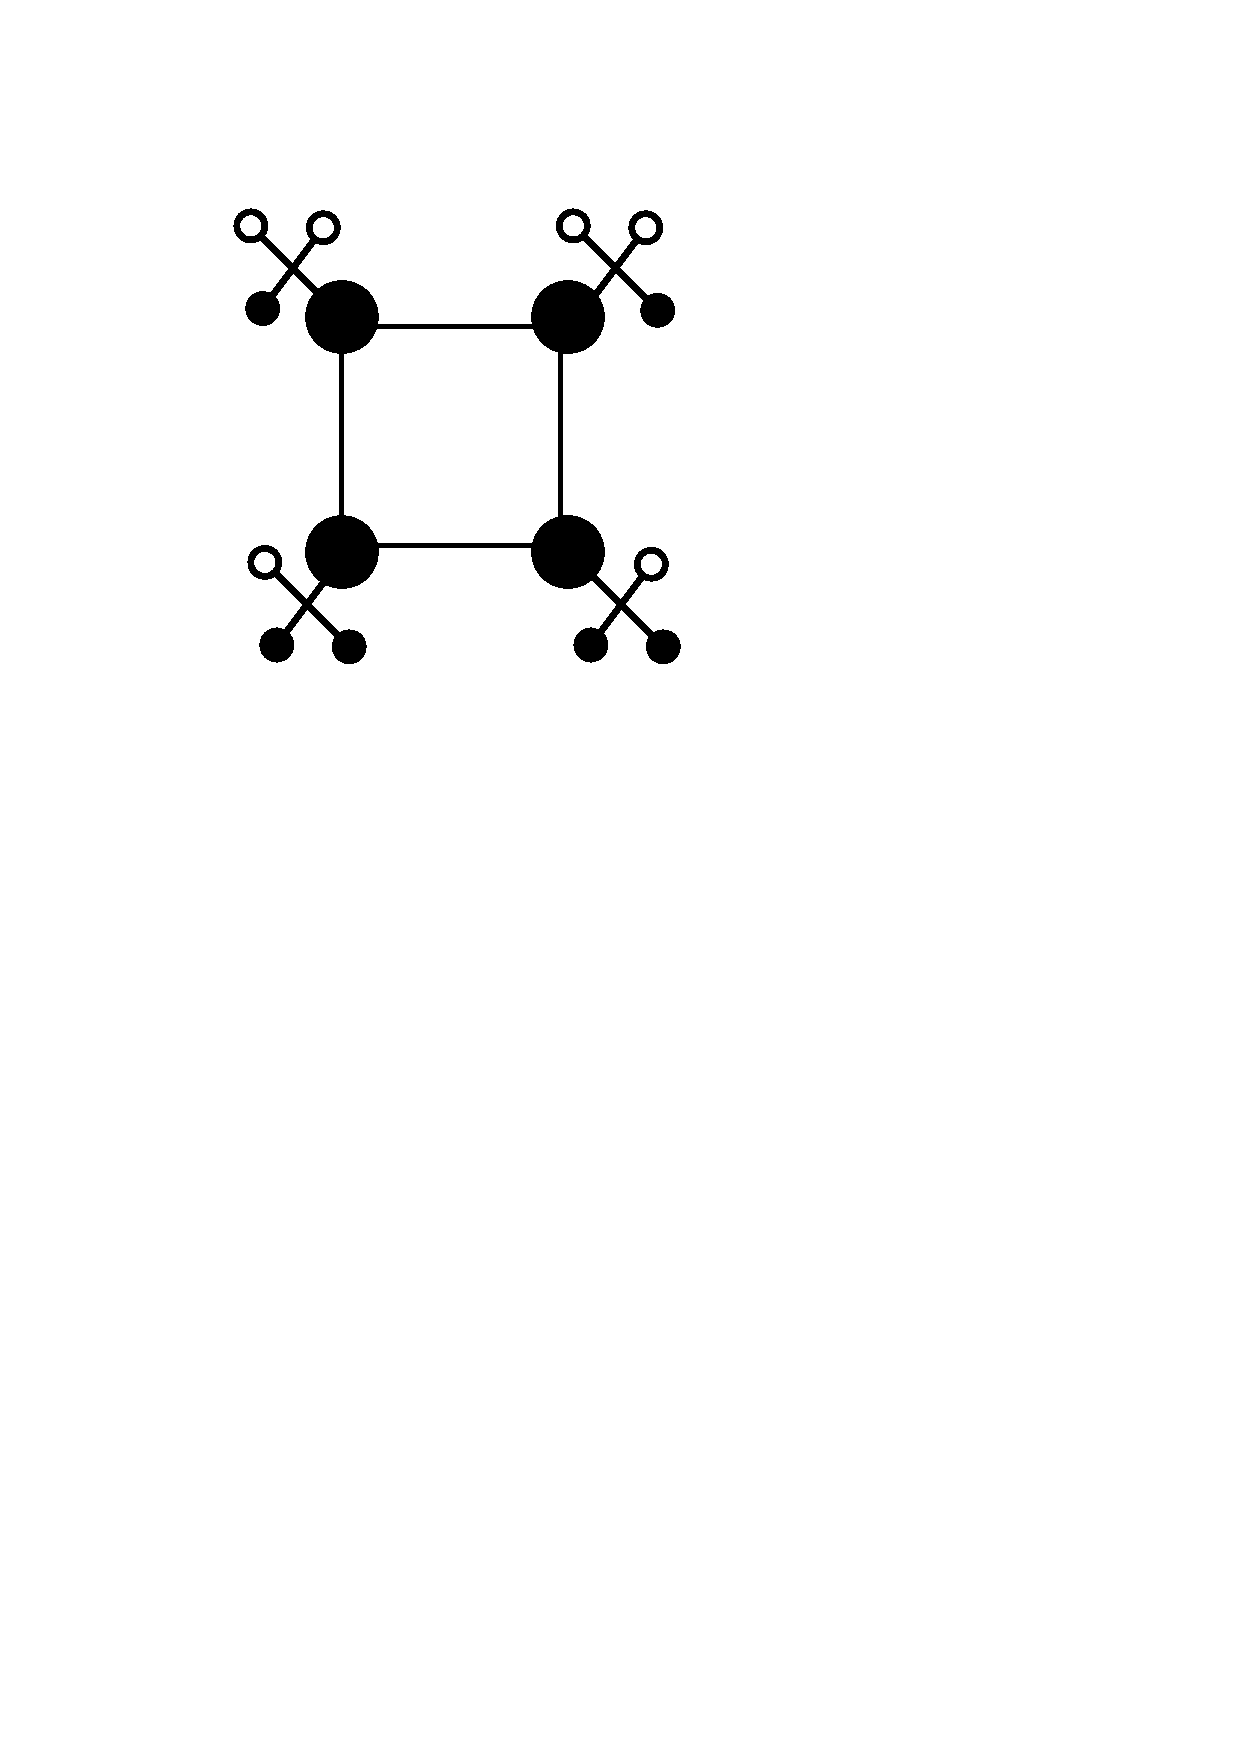
\includegraphics[trim=LEFT BOTTOM RIGHT TOP, clip, width=0.9\textwidth,]{resources/pdfs/EXAPLATONICFORM-PFA.pdf}\\
   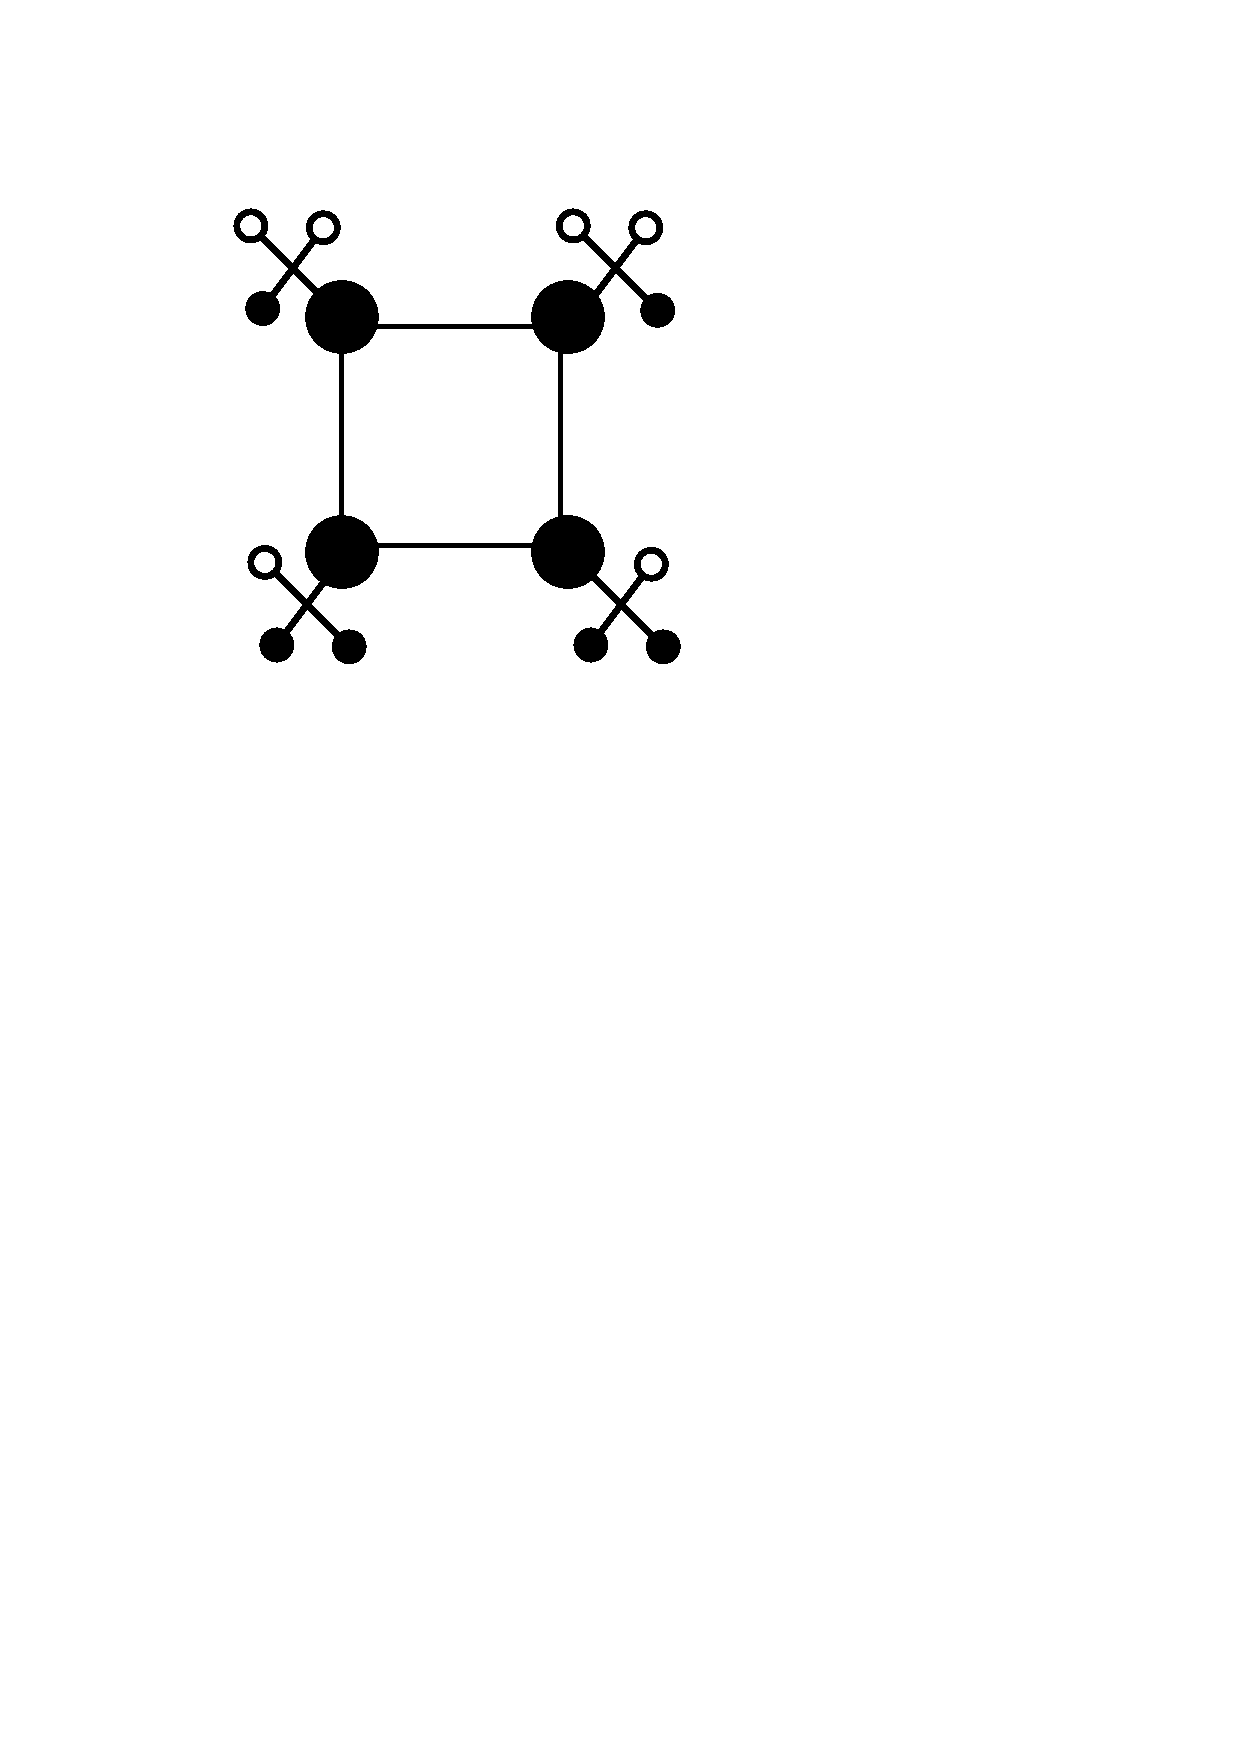
\includegraphics[trim=3cm 18cm 8cm 3cm, clip, width=0.9\textwidth,]{resources/pdfs/EXAPLATONICFORM-PFA.pdf}\\
   \caption{An example of a single \textbf{amino-acid} or rather, the \textbf{PFA} component of a \textbf{FGE} equivalent to one \textbf{amino-acid} segment expressed using the \textbf{LGES} system. This particular expression corresponding to a rendering of the configuration \textbf{$4_{pf} \otimes 6_{oz}$} = \textbf{$4_{pf} + 4 \times 6_{oz}$}.}
  \label{FIGEXAPLATONICFORMPFA}
  \end{center}
\end{figure}



After looking at some examples of actual genome expressions rendered using the \textbf{LGES}, perhaps most reviewers of \textbf{\hyperref[ALGCOZINPLATO]{Algorithm \ref{ALGCOZINPLATO}}} shall come to appreciate that it is not only non-trivial, but is likewise plausible given the sensibilities of how actual expression occurs in nature/reality\footnote{That said, it shall be up to others --- botanists, zoologists, molecular biologists, virologists, etc. to either confirm or refute whether or not \textbf{LGES} does indeed echo the reality in nature or whether it is a theory only applicable to a subsection of reality --- \textit{which if not all?}} --- see a natural expression as in \textbf{\hyperref[FIGPINEAPPLE]{Figure \ref{FIGPINEAPPLE}}}, and that it encapsulates the ideals of both distinctiveness but also diversity for the minutest of organic creatures that are just as basic as mere genetic code with a basic encapsulating body (such as viruses), but also complex organisms belonging to distinct families of prokaryotes and eukaryotes.


\subsection{Examples of Complete Lu-Genome Expressions}
\label{SECFULLGES}


We get to see the first example of the output of processing some na-Sequence expressed originally in base-$\Omega$ such as for $\Omega_{3}$ from \textbf{Equation \ref{EQDNEXA}}, in its final expression form as in \textbf{Figure \ref{FIGPLATONICEXA}}\cite{lutalo_2025_exa} --- more importantly, since we have already seen its \textbf{IFA} (the \textbf{FGE} prefix) in \textbf{Figure \ref{FIGOZEXA}}, we note that we essentially see the update as the result of expressing the entire \textbf{FGE} via the \textbf{IFA MSS} equivalent to the following derivation transformation:

\begin{center}
\fbox{
\begin{minipage}{\textwidth}

\begin{trans}
\label{TRANSFGEDERIV}
$\Omega_{3} = \langle 0,1,2,3,0,2,6 \rangle \rightarrow \overset{>}{\Omega_{3}} = \langle 0, 2, 1, 3, 6 \rangle$\\
$ \implies m = \invpi(\overset{>}{\Omega_{3}}) = 5 \implies  \boxed{\psi_{pf}}_5 = \langle 2, 1, 0, 6, 8 \rangle$\\ 
$\implies \boxed{OZ(\Omega_{3})} = \langle 2_{pf} \otimes 0_{oz}, 1_{pf} \otimes 2_{oz}, 0_{pf} \otimes 1_{oz}, 6_{pf} \otimes 3_{oz}, 8_{pf} \otimes 6_{oz} \rangle$\\\\
$ \approx \langle GAP, 1_{pf} \otimes 2_{oz}, GAP, 6_{pf} \otimes 3_{oz}, 8_{pf} \otimes 6_{oz} \rangle$\\\\
$\implies \boxed{OZ(\Omega_{3})}^* = \langle 0,1,2,3,0,2,6 \rangle_{oz} \cdot \langle GAP, 1_{pf} \otimes 2_{oz}, GAP, 6_{pf} \otimes 3_{oz}, 8_{pf} \otimes 6_{oz} \rangle$
\end{trans}


\end{minipage}}
\\
\end{center}


The corresponding complete rendered \textbf{FGE} for $\Omega_{3}$ would then be as shown in \textbf{Figure \ref{FIGPLATONICEXA}}.



\begin{figure}[H]
  \begin{center}
  %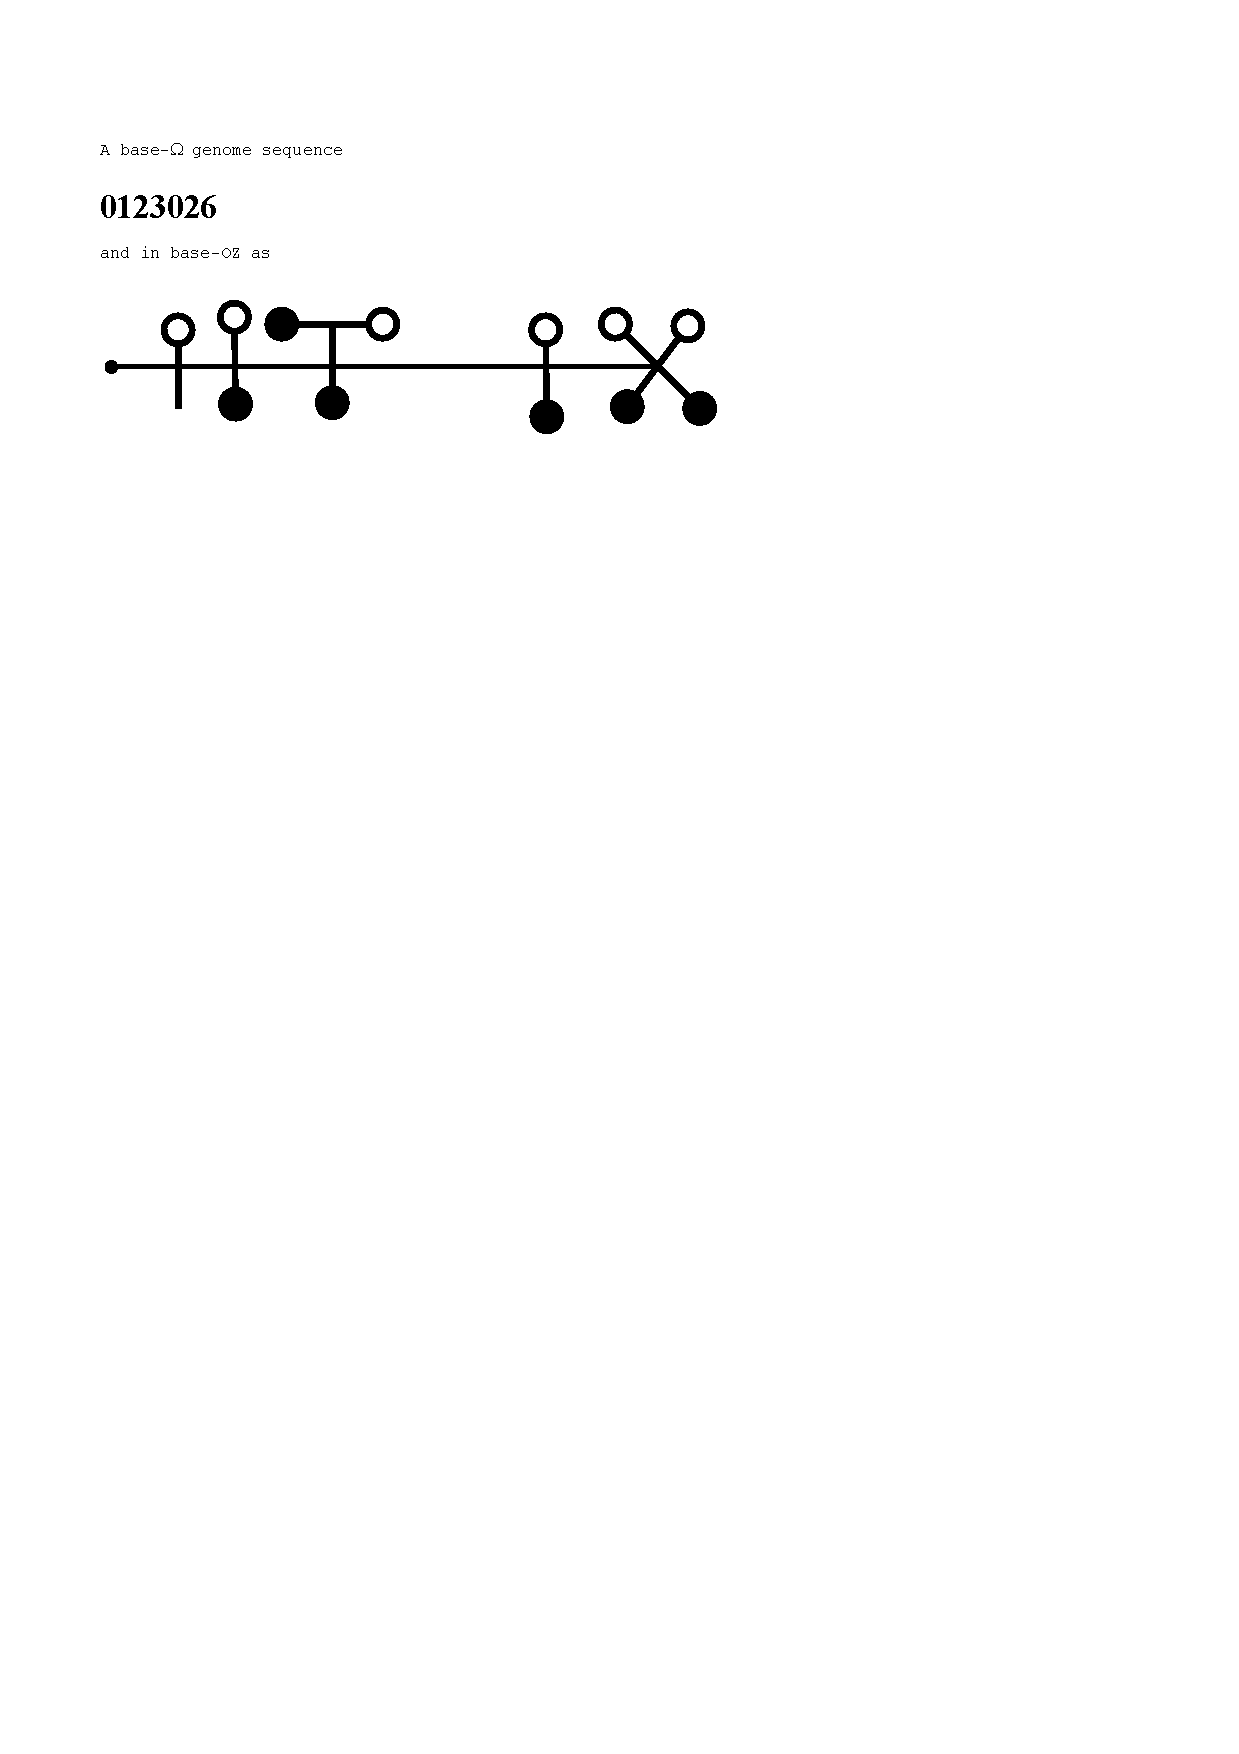
\includegraphics[trim=0cm 20cm 0cm 0cm, clip, width=0.9\textwidth,]{resources/pdfs/OZINCIPHER-APP3-EXA.pdf}\\
   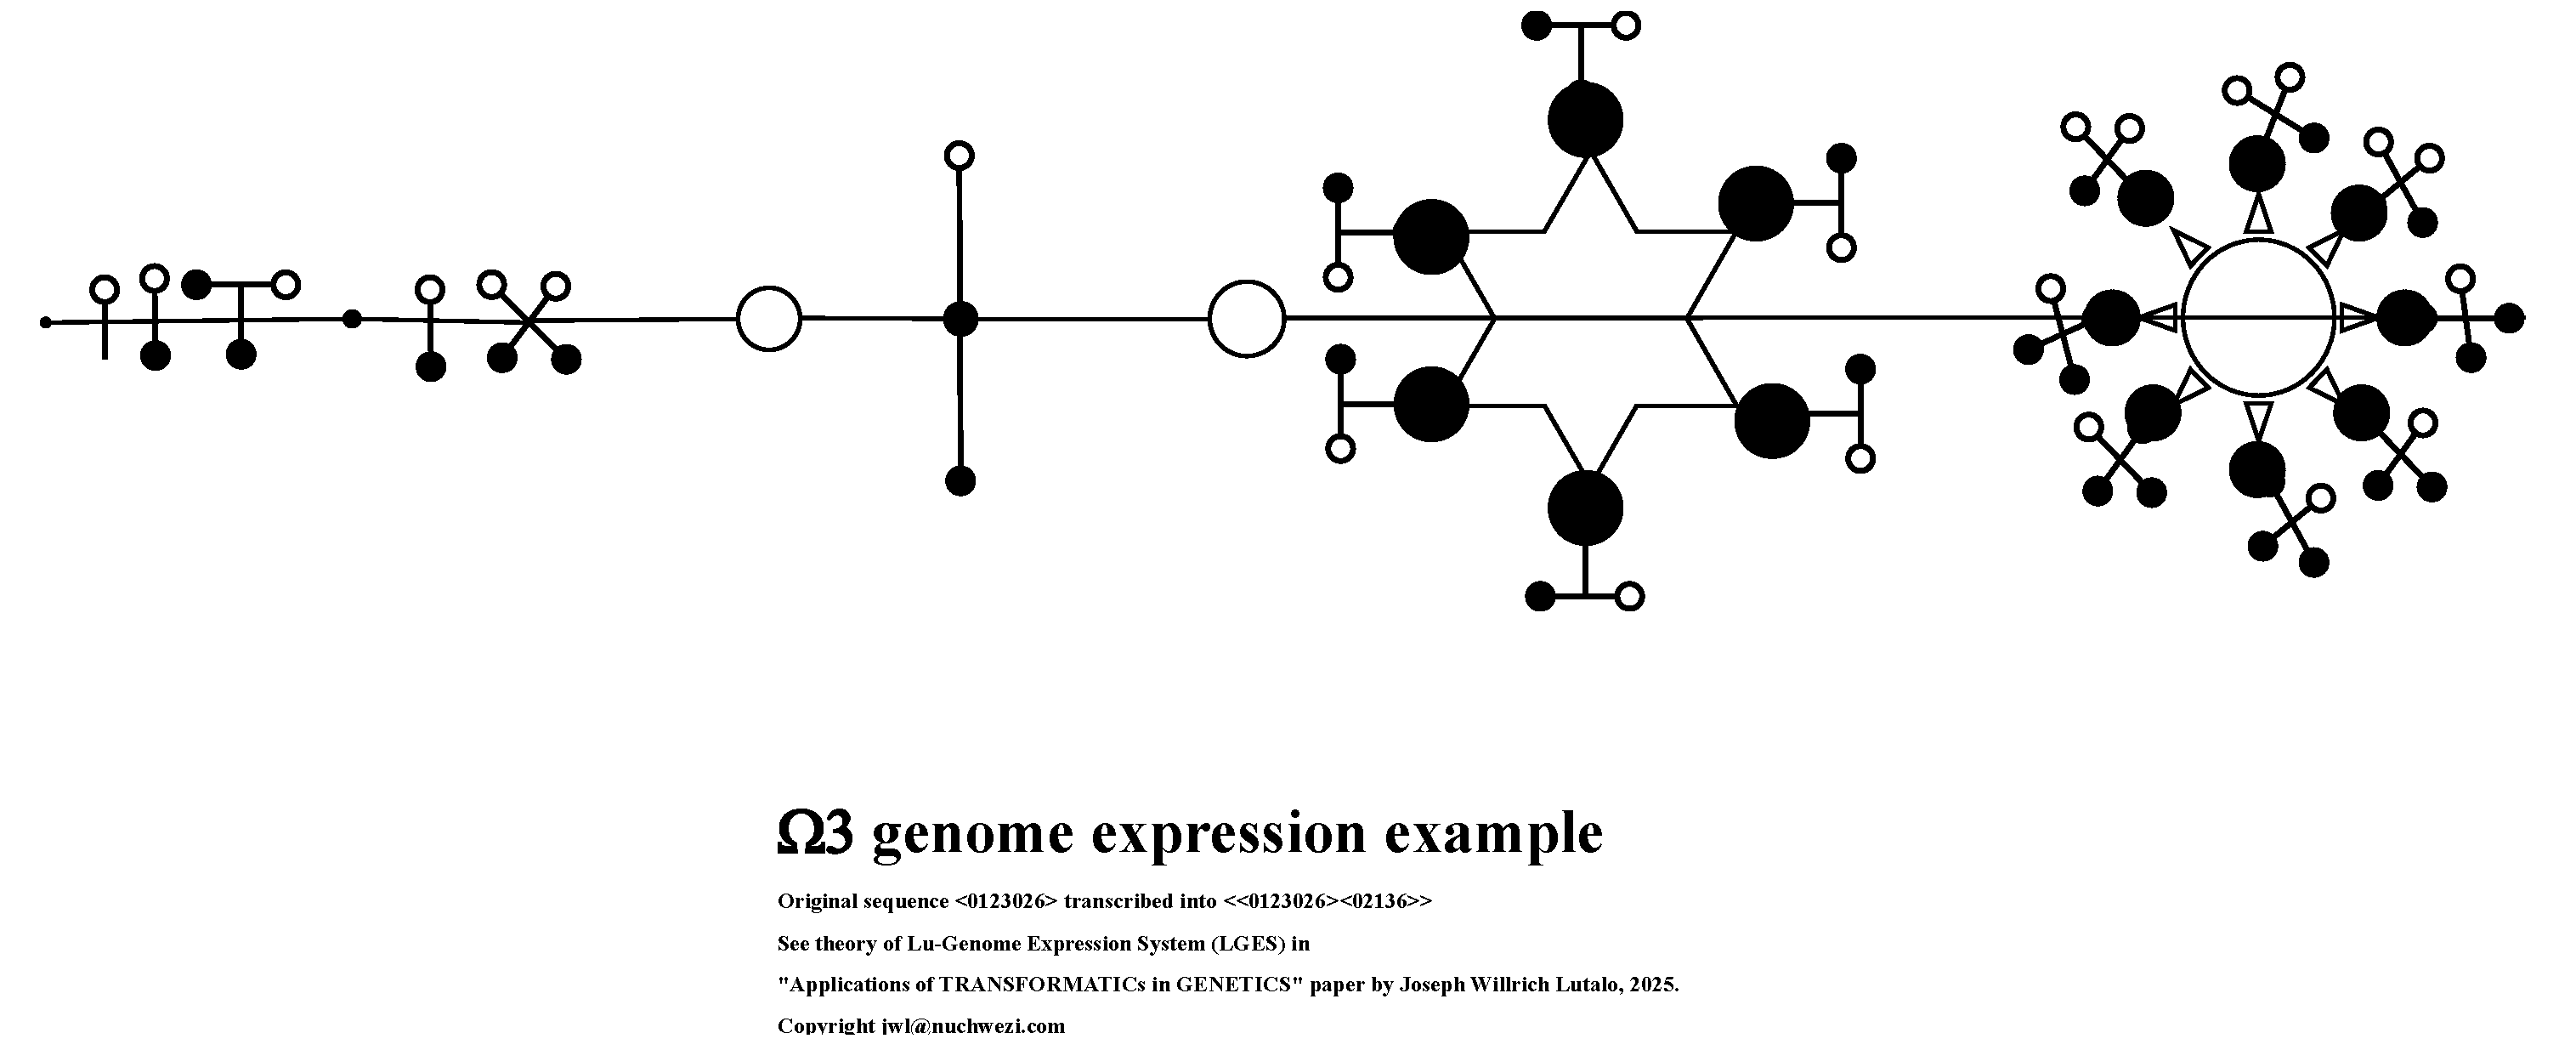
\includegraphics[trim=0cm 0cm 0cm 0cm, clip, width=0.9\textwidth,]{resources/pdfs/PLATONIC-EXA-landscape.pdf}\\
   \caption{The equivalent LGES complete genome expression of the $\Omega_{3}$ genome sequence (from \textbf{Equation \ref{EQDNEXA}})}
  \label{FIGPLATONICEXA}
  \end{center}
\end{figure}


Though we won't delve into exploring all kinds of possible \textit{interesting} scenarios with regards to the \textbf{LGES}, we can look at one other example and then move on. Also, it shall be interesting and worth noting --- especially for those who wish to explore the \textbf{LGES} algorithm, that a mathematical derivation such as depicted in \textbf{\hyperref[TRANSFGEDERIV]{Transformation \ref{TRANSFGEDERIV}}}, captures the gist of all there is to \textbf{LGES}, and that any other case can merely adapt such a formalism so as to arrive at the visual/pictorial expression of some $\Omega$-encoded genetic or arbitrary sequence.


From the example hypothetical genome sequences we have encountered, perhaps let us revisit \textbf{\hyperref[EQDNAV]{Equation \ref{EQDNAV}}} and see what the \textbf{Euler Virus} might look like when fully expressed in our system.

So, first of all, note that we already did the first-leg of \textbf{\hyperref[ALGCOZINPLATO]{Algorithm \ref{ALGCOZINPLATO}}}, and we have seen what the \textbf{FGE} prefix --- the \textbf{IFA}, would look like in \textbf{Figure \ref{FIGOZEVIRUS}}\footnote{Talking of which, for the well-read reader, and especially students and explorers of not just esoteric languages but especially occult languages and systems --- perhaps better we talk of \textbf{Occult Philosophy}\cite{agrippa2014occult}, not only the coincidence that our OZIN-expressions look indeed \textit{occult} --- such as one might find utilized in occult systems such as John Dee's Enochian\cite{lutalo2025unraveling}, but also that both the \textbf{IFA} and \textbf{PFA} --- the later, expressed in a somewhat more familiar (because the polygons at the core of the PF-cipher are indeed commonplace in both mathematics and mysticism) language, but ultimately, the experienced observer might appreciate that complete \textbf{LGES} expressions/figures such as \textbf{Figure \ref{FIGPLATONICEXA}} look much like the traditional/ancient mystical glyphs known as \textbf{Mandalas} to modern scholars such as Carl G. Jung that enjoyed these subjects\cite{jung1964symbols} and perhaps, and as the author himself has explored in works such as the novel ``Rock `N' Draw"\cite{lutalo2025rock}, these figures so much remind one of \textbf{Voodoo Veves} --- in that novel, depicted as enchantment geomantic/geomancy forms! Perhaps, in a later work on either philosophy or mysticism by the author --- see earlier works of this kind in \cite{lutalo2025concerning_trans}, we shall want to take time off and properly explore this exciting dimension of human expression and culture, especially since, unlike what might have ever come before, our symbolic programs, unlike voodoo veves or chaos magick sigils, are rooted in two objective fields of inquiry --- mathematics and biology (and not mere speculation). And no, though the acronym \textbf{IFA} reminds one of the \textit{Ifa} esoteric system of  Western Africa, and yet, the author didn't have that in mind while working on the LGES at first.}. So, like we did for $\Omega_{3}$ in the last exploration, let us start by looking at what the numeral-equivalence of the processed $\Omega_{veuler}$ would be like. For brevity, we can sum up the entire production/transformation that leads to the complete \textbf{FGE} with correct prefix and suffix, and thus $\boxed{OZ(\Omega_{veuler})}^*$ as:

\begin{center}
\fbox{
\begin{minipage}{\textwidth}

\begin{trans}
\label{TRANSGENSEQEVIRUS}
$\Omega_{veuler} = \langle 2,7,1,8,2,8,1,8 \rangle \rightarrow \hbar(\overset{>}{\Omega_{veuler}}) = \text{\textbf{8}3\textbf{2}2\textbf{1}2\textbf{7}1} \rightarrow \overset{>}{\Omega_{veuler}} = \langle 8, 2, 1, 7 \rangle \implies  m = \invpi(\overset{>}{\Omega_{veuler}}) = 4 \implies  \boxed{\psi_{pf}}_4 = \langle 1, 6, 4, 7 \rangle$\\
$\implies \boxed{OZ(\Omega_{veuler})} = \langle 1_{pf} \otimes 8_{oz}, 6_{pf} \otimes 2_{oz}, 4_{pf} \otimes 1_{oz}, 7_{pf} \otimes 7_{oz}\rangle$\\\\
$\implies \boxed{OZ(\Omega_{veuler})}^* = \langle 2,7,1,8,2,8,1,8 \rangle_{oz} \cdot \langle 1_{pf} \otimes 8_{oz}, 6_{pf} \otimes 2_{oz}, 4_{pf} \otimes 1_{oz}, 7_{pf} \otimes 7_{oz} \rangle$


\end{trans}

\end{minipage}}
\\
\end{center}


Note that in that derivation depicted in \textbf{\hyperref[TRANSGENSEQEVIRUS]{Transformation \ref{TRANSGENSEQEVIRUS}}}, one of the most tricky parts is computing that FGE suffix, $\boxed{OZ(\Omega_{veuler})}$, the \textbf{PFA} --- which is formalized/defined by \textit{especially}\footnote{\textbf{\hyperref[EQEXTFGEJOINTSUF]{Equation \ref{EQEXTFGEJOINTSUF}}} is what covers the special symbol `0', that is treated as a JOINT/GAP in the \textbf{PFA} and as STOP/GAP in \textbf{IFA}.} \textbf{\hyperref[EQFBOXED]{Equation \ref{EQFBOXED}}}. So, once that is done, and we have our final numeral-\textbf{FGE} as such:\\

\begin{equation}
\label{EQGFEEVIRUS}
\boxed{OZ(\Omega_{veuler})}^* = \langle 2,7,1,8,2,8,1,8 \rangle_{oz} \cdot \langle 1_{pf} \otimes 8_{oz}, 6_{pf} \otimes 2_{oz}, 4_{pf} \otimes 1_{oz}, 7_{pf} \otimes 7_{oz} \rangle
\end{equation}\\

Of course, concerning \textbf{\hyperref[EQGFEEVIRUS]{Equation \ref{EQGFEEVIRUS}}}, note that, or rather, keep in mind that concerning the \textbf{PFA} component, $\boxed{OZ(\Omega_{veuler})}$, the corresponding associated sequence in numeral form is the \textbf{IFA MSS}, $\overset{>}{OZ(\Omega_{veuler})} = \overset{>}{\Omega_{veuler}} = \langle 8, 2, 1, 7 \rangle$. And thus, using \textbf{the necessary} transcription and translation ciphers as well as the multiplication/linear-combination rules required by \textbf{\hyperref[EQFBOXED]{Equation \ref{EQFBOXED}}} when treating of the \textbf{PFA}, we then generate the final genome expression for the \textbf{Euler Virus} under the \textbf{LGES} that looks as in \textbf{Figure \ref{FIGLGESEULERVIRUS}}.


\begin{figure}[H]
  \begin{center}
  %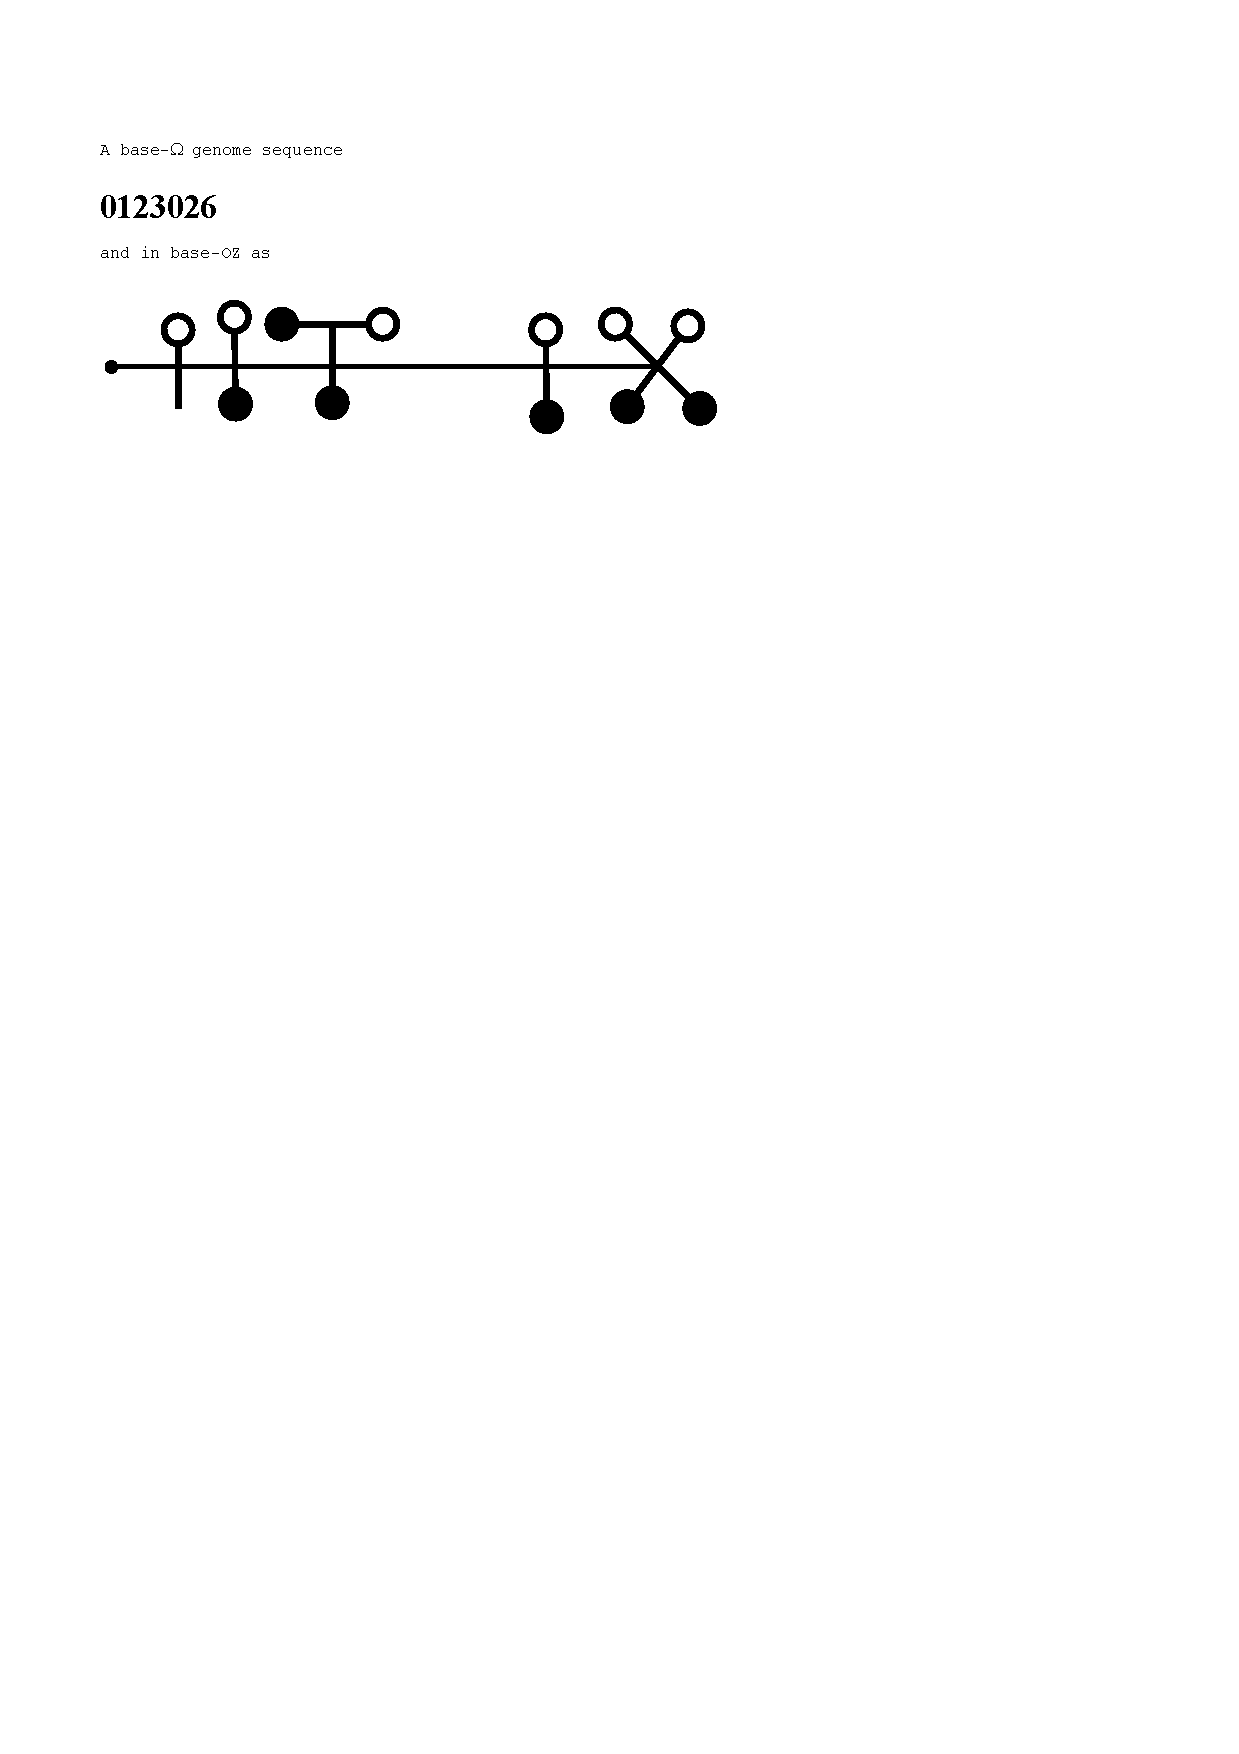
\includegraphics[trim=0cm 20cm 0cm 0cm, clip, width=0.9\textwidth,]{resources/pdfs/OZINCIPHER-APP3-EXA.pdf}\\
   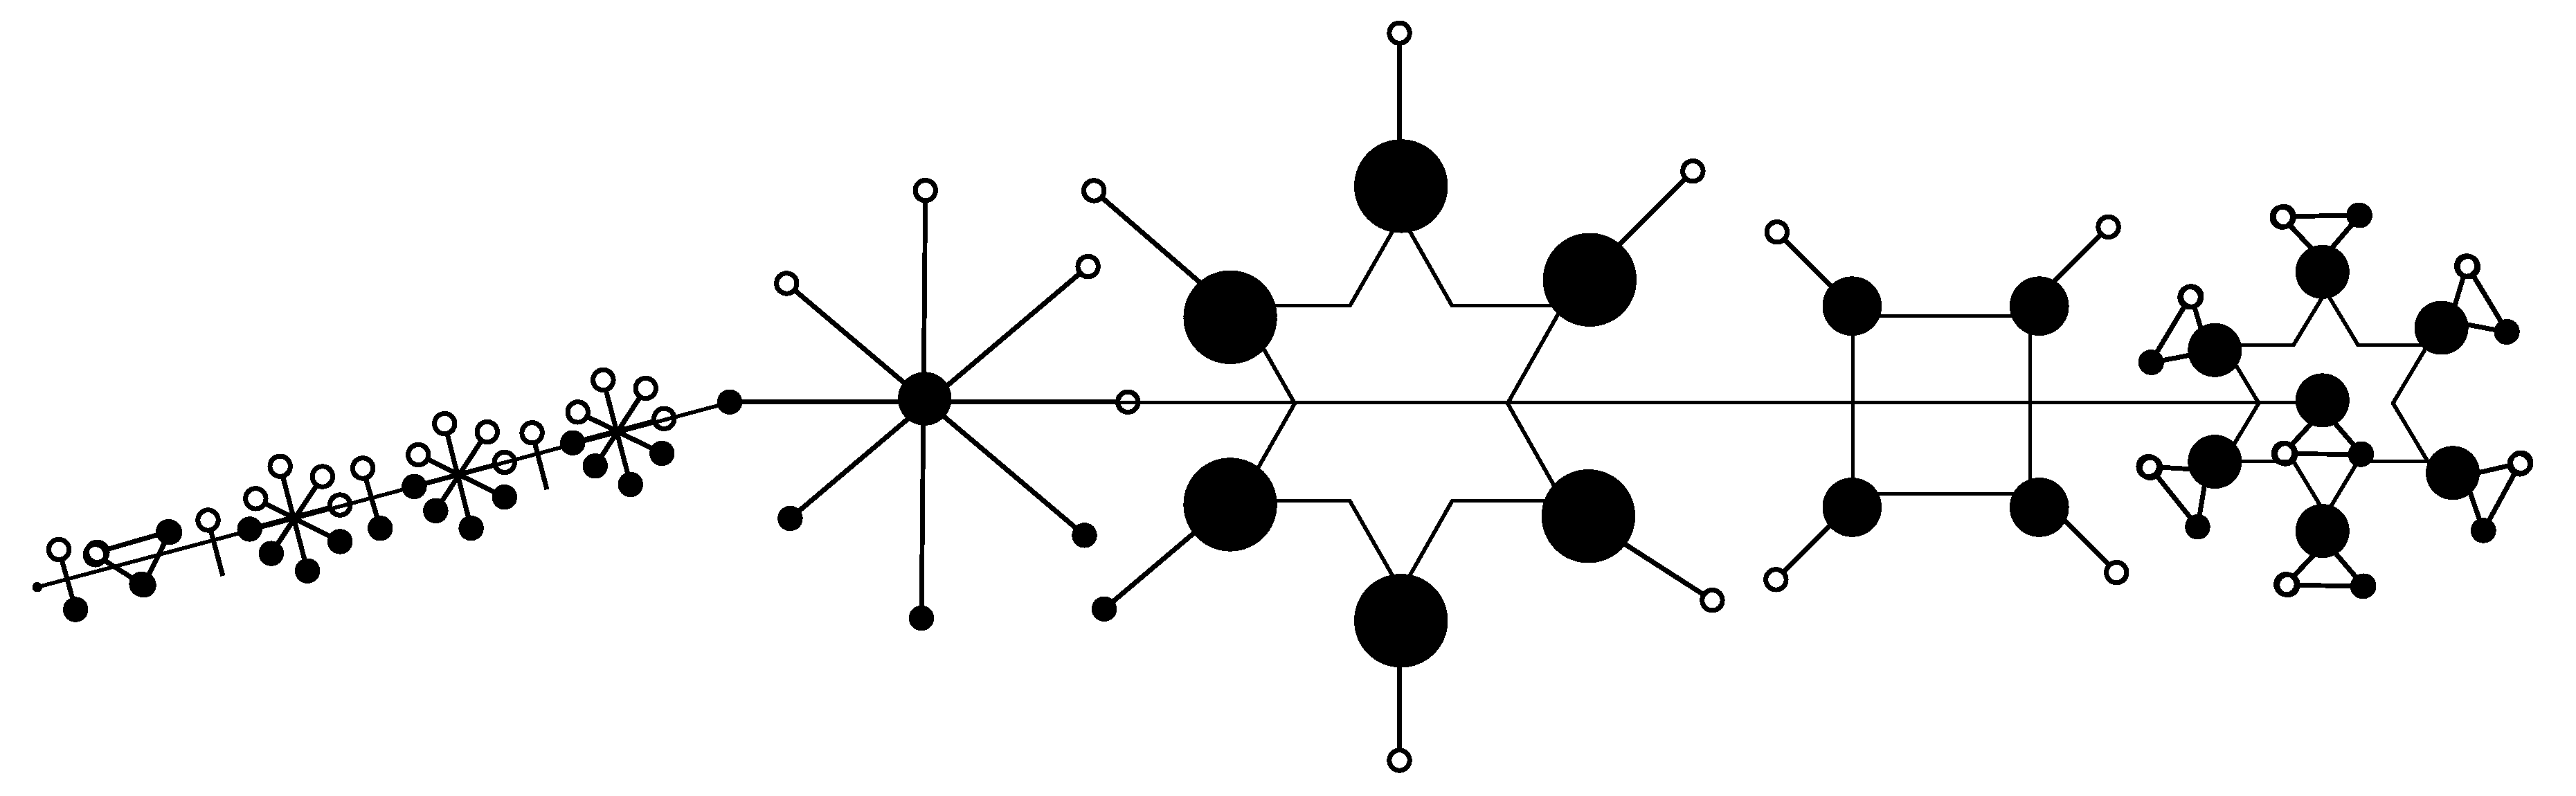
\includegraphics[trim=0cm 0cm 0cm 0cm, clip, width=0.9\textwidth,]{resources/pdfs/PLATONIC-EULERVIRUS-landscape.pdf}\\
   \caption{The equivalent LGES complete genome expression of the $\Omega_{veuler}$ (Euler Virus) genome sequence (from \textbf{Equation \ref{EQGFEEVIRUS}})}
  \label{FIGLGESEULERVIRUS}
  \end{center}
\end{figure}


Now, concerning that rendering of the genome sequence expressed in \textbf{Equation \ref{EQGFEEVIRUS}}, it might be worth noting that unlike the earlier examples of \textbf{LGES} expressions, we have taken the liberty to exploit that special joint that kick-starts the \textbf{PFA}, or rather, which separates the \textbf{IFA} from the \textbf{PFA} in a \textbf{FGE} expression. So, just like an organism with a physical joint might sometimes appear as angled or curved, so we have chosen to depict the $\Omega_{veuler}$ with its one joint\footnote{Definitely, and interesting to explore, a genome sequence with multiple JOINT points in it might be how an organism with say appendages such as legs, hands and a head that can move independently of the core/thorax of the body is possibly arrived at. The interested student should go ahead and explore more non-trivial $\Omega$-base sequences just to see what's possible.} well utilized. However, and important to note; it is not just joints that might appear different across different renderings of the same basis genome sequence. So, in \textbf{Figure \ref{FIGLGESEULERVIRUSv2}}, we see another rendering of the same genome sequence expression, with readily noticeable differences being the IFA-PFA joint in its neutral position (we also simplified and fused it with one of the edge-nodes of the $1_{pf} \otimes 8_{oz}$ term in both diagrams), and then the second term in the PFA (corresponding to \textbf{$7_{pf} \otimes 2_{oz}$} or rather \textbf{$7_{pf} + 7 \times 2_{oz}$}) with the $2_{oz}$ appendages depicted mostly aligned horizontally --- basically, there's still room for some creativity while rendering, but perhaps the future and more research might help decide on what is optimal/ideal. At the moment, its mostly the mathematics and sane principles of design and trusting that in nature, systems are at there basic form when in states of lowest kinetic energy or highest potential energy\footnote{Such as, not finding trees that grow with their stems at an angle to the ground or animals with curved legs or walking on 3 legs or with the legs all at the back for 4-legged animals, etc... Though we didn't cite any authority on this matter, we trust that basic physics applied to anatomy and physiology might help justify the sensibilities we only seem to be applying from basic understanding of physics and nature here.}.


\begin{figure}[H]
  \begin{center}
  %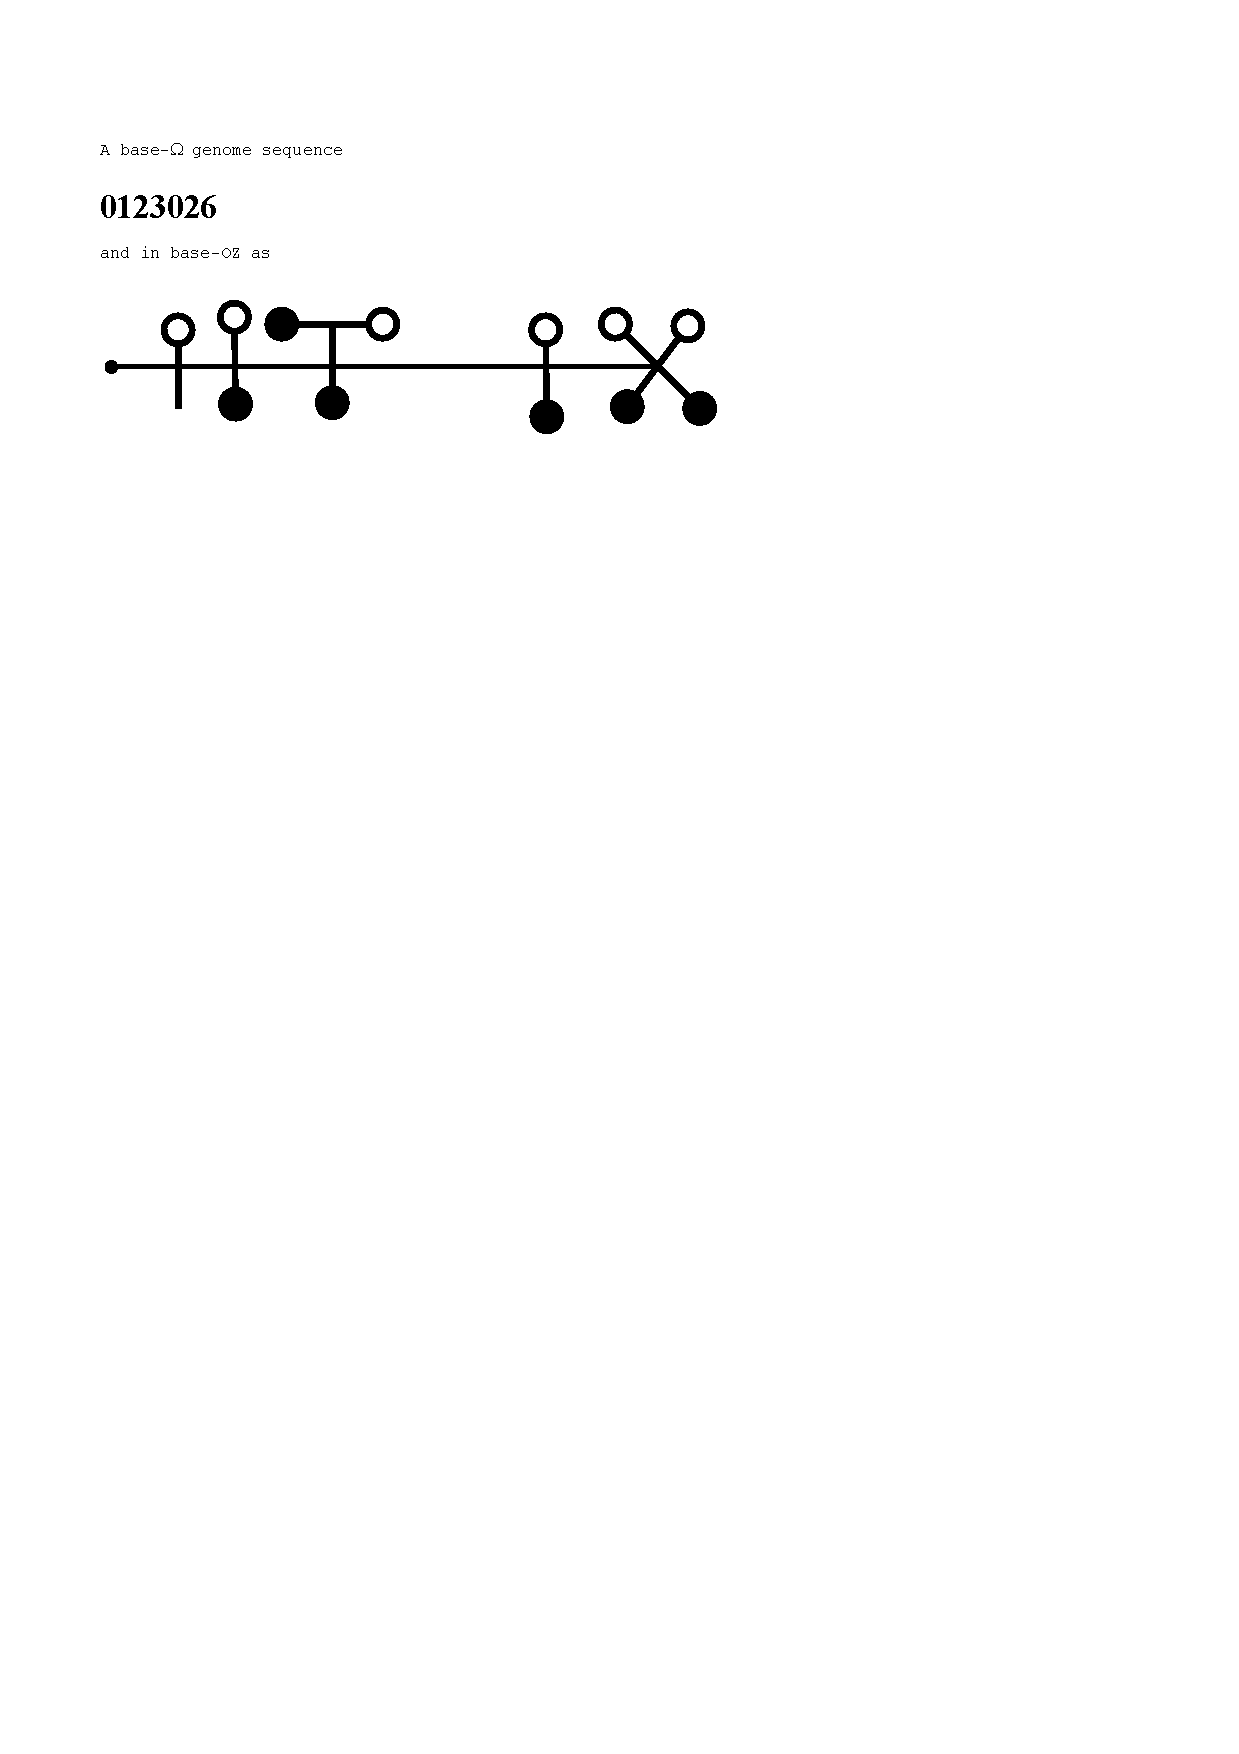
\includegraphics[trim=0cm 20cm 0cm 0cm, clip, width=0.9\textwidth,]{resources/pdfs/OZINCIPHER-APP3-EXA.pdf}\\
   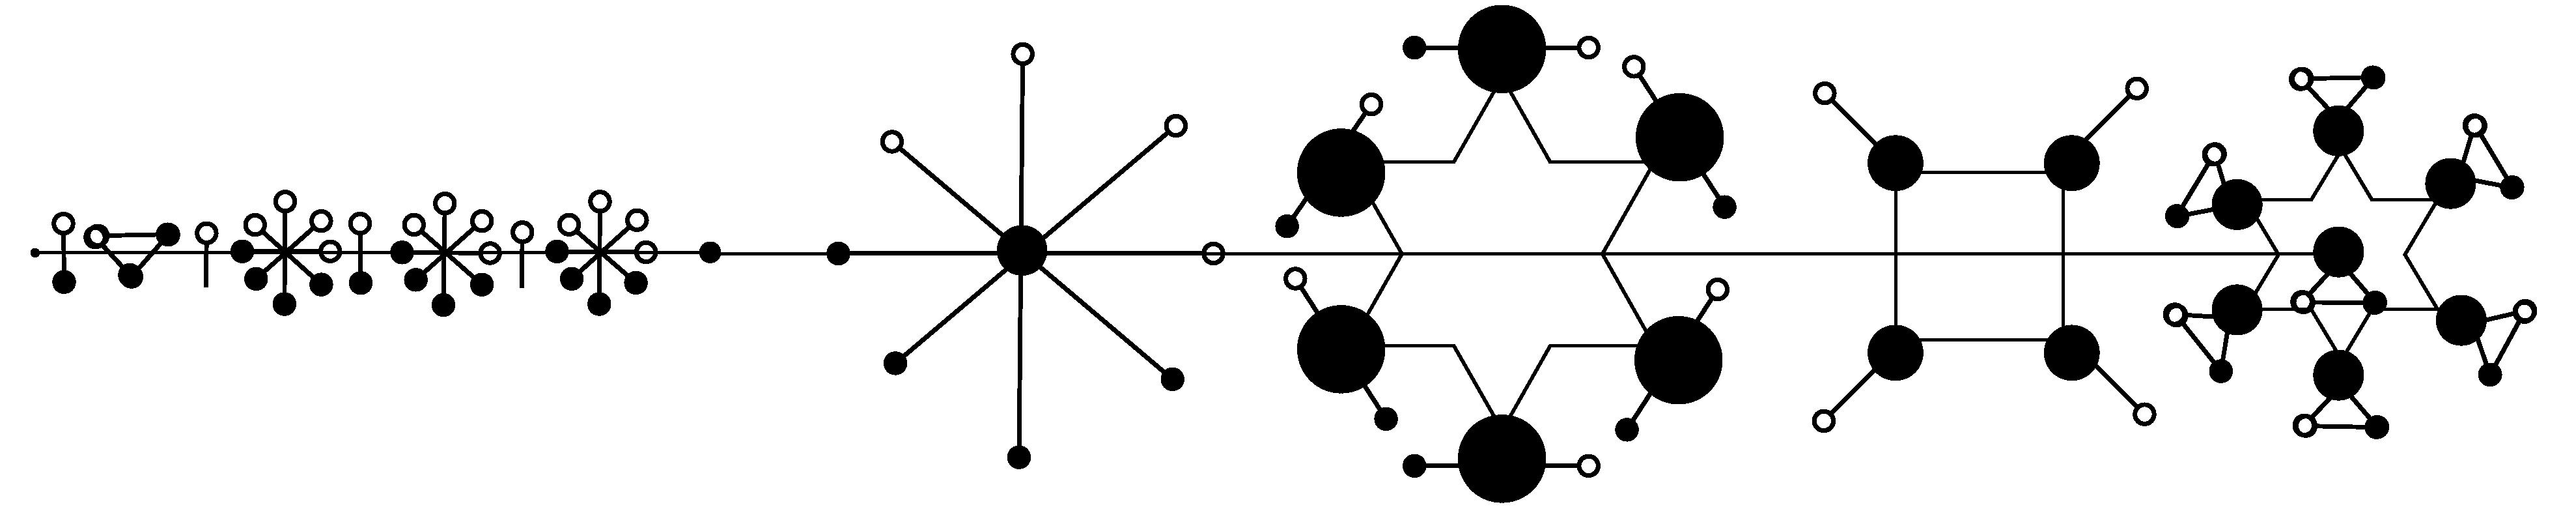
\includegraphics[trim=0cm 0cm 0cm 0cm, clip, width=0.9\textwidth,]{resources/pdfs/v2-PLATONIC-EULERVIRUS-landscape.pdf}\\
   \caption{An \textbf{alternative rendering} of the same sequence as $\Omega_{veuler}$ originally depicted as the \textbf{LGES} genome expression in \textbf{\hyperref[FIGLGESEULERVIRUS]{Figure \ref{FIGLGESEULERVIRUS}}}}
  \label{FIGLGESEULERVIRUSv2}
  \end{center}
\end{figure}

And talking of scaling nodes, in the future, we might want to explore whether in such a system as \textbf{LGES} in which the expression is sensitive to measures such as the \textbf{IFA MSS}, whether it might make sense to scale each subsequent pf-node in the \textbf{PFA} based on its position within the sequence? Though we didn't have such a rule included in \textbf{\hyperref[ALGCOZINPLATO]{Algorithm \ref{ALGCOZINPLATO}}}, and yet, our example renderings here have somewhat taken advantage of that plausible logic.

That said, note that we started this work with a photograph of a pineapple ready to harvest (see \textbf{Figure \ref{FIGPINEAPPLE}}), and though the associated discussion\footnote{Checkout video/mini-lecture concerning this particular organism and what might be gleaned about genetic expressions from it, via author's YouTube: \url{https://youtube.com/shorts/yTJzBEpw7Z4}} did bring up the matter of how it might inspire a genome expression system in which the prefix is the actual DNA that renders the rest of the organism (fruit, plant-base and roots in this case of the pineapple), it is left as an exercise to the reader to decide whether example genome sequence expressions/renderings such as in \textbf{Figure \ref{FIGLGESEULERVIRUS}} depict this pineapple-inspired philosophy.


\begin{center}
\fbox{\begin{minipage}{0.9\textwidth}
\large
\textbf{NOTE:}\\
 On \textbf{Why Place-Notation Expression Systems Matter} \\

As a further justification for why we chose to use a place-notation sensitive genetic code expression system in our conceptual genome expression thought experiment, consider that, just like with modern numbers and number sysems --- of which the Arabic number system is considered one of the best since ancient times, the appearance of a symbol within an expression is interpreted not just by what it quantifies, but also by where in the expression it is situated. 

For good measure, a few enlightening quotes from the priceless work on the evolution of number systems since ancient times, by Raymond S. Nickerson, shall help cement this:

\begin{quotation}
\noindent \texttt{Aristotle attached considerable significance to the fact that human beings can count: it is this ability, he claimed, that demonstrates our rationality.}\\\\

\noindent \texttt{As Brainerd (1973) has pointed out, in most Western nations today we expect students, by the time they reach their early teens, to be much more competent with numbers than was an educated adult Greek or Roman of 2,000 years ago. This fact arises in no small measure from the elegance and power of the scheme that we now use to represent numbers.}\\\\


\noindent \texttt{In short, a price of the increased abstractness of the Arabic system is an obscuring of some of the key principles on which numbers are based. To an ancient Egyptian, the fact that 3+4=7 was apparent from the relationship between the Egyptian number representing 7 and those representing 3 and 4. There is no hint of such a relationship, however, when this equation is expressed in Arabic notation. The price has been worth the paying, however.}\\\\


\noindent \texttt{If you invented a unique symbol to represent each of the possible quantities of stones (including the case of no stones) up to that of your standard and decided to use the position of that symbol to indicate the pile to which it refers, you would have what we refer to today as a place-notation system for representing numbers.}\\\\

\noindent \texttt{The relative ease with which one can count or compute depends to no small degree on the characteristics of the system that is used to represent number concepts.}\\

\hspace*{\fill} ---\textbf{Raymond S. Nickerson}, \textit{Counting, Computing, and the Representation of Numbers}, 1988\cite{nickerson1988counting}
\end{quotation}

And finally, it shall be worth noting that this notion also underlies the present author's use of the \textbf{Position-Index measure} ($I(\omega_i, \Theta)$), first formalized in the Base-36 paper\cite{base36paper}, and which, among many important applications it has, is its use in generalizing the computation of decimal values of arbitrary number expressions in any base, its use in transformatics to express sequence summaries using modal sequences\cite{transformatics}, etc.

\end{minipage}}
\\
\end{center}


\section{The Extended Lu-Genome Expression System (x-LGES)}
\label{SECxLGES}

If you look at the genome sequence expressions that we have encountered in \textbf{\hyperref[SECFULLGES]{Section \ref{SECFULLGES}}}, and compare that to the case of our pineapple in \textbf{\hyperref[FIGPINEAPPLE]{Figure \ref{FIGPINEAPPLE}}} that opens the introduction section, you shall notice that, just in case we assume our \textbf{LGES} protocols to be sufficient for the expression of not just bits of an organism, but also relevant to the expression of \textbf{the complete organism}, then, it might seem like something is still missing, and thus the \textbf{Extended Lu-Genome Expression System} (x-LGES).


So, what exactly is missing from our genome expressions thus far? We shall call out a few telling points to help drive the point home:

\begin{enumerate}
\item As has been stressed already, and as is the case that we wish our science to not be constructed in ivory towers alienated from facts and reality in nature, we must borrow a leaf from how actual DNA is utilized to express organisms in reality. For example, it is not that one genome expresses the hands, another the heart, and yet another the eyes! Well, of course, in a particular organism's DNA, there shall be specific subsequences that best define the expression of particular features or aspects of an organism, however, overall, a single, complete genome sequence is and should be sufficient for the complete expression of an entire organism with all its various attributes and distinct aspects well catered for.
\item When we consider the way the original \textbf{LGES} algorithm is specified --- \textbf{\hyperref[ALGCOZINPLATO]{Algorithm \ref{ALGCOZINPLATO}}} being the one that combines both transcription and translation into a single process, we shall note that, the final output of that process --- as depicted in \textbf{\hyperref[EQTRANSLGENSEQ]{Equation \ref{EQTRANSLGENSEQ}}} for the general case, and as in \textbf{\hyperref[EQGFEEVIRUS]{Equation \ref{EQGFEEVIRUS}}} for one particular organism's expression (in \textit{numerical form}), we notice that, especially when approached from the point of view of the fully-processed rendering of the \textbf{FGE}, $\boxed{OZ(\Theta_\Omega)}^*$, some potentially relevant information could be considered to be \textit{missing}\footnote{Well, technically, unless when one is only studying the visual expressions corresponding to a particular genome sequence --- which might introduce a lot of variations and exploit a lot of creative freedom, when we instead express the genome in the mathematical form as in \textbf{\hyperref[EQGFEEVIRUS]{Equation \ref{EQGFEEVIRUS}}}, almost all the necessary information about the genome is present at that moment, including the important statistical summary information from the \textbf{IFA MSS}.} from that expression at that point. In particular, when we have the \textbf{PFA} expressed in its platonic form, it might not readily be possible to discern the vital $\overset{>}{OZ(\Theta_\Omega)}$ aspect since the actual \textbf{PFA} is a combination (see \textbf{\hyperref[EQFBOXED]{Equation \ref{EQFBOXED}}}) of that \textbf{IFA MSS} in its OZIN form as well as its translation into complementary Platonic Form expressions via the \textbf{\hyperref[FIGPLATONICCIPH]{PLATO CIPHER}}.
\item Finally, and again, returning to nature as our authority on genome expression, we note that most organisms --- plants or animals, typically manifest in a \textbf{PREFIX-THORAX-SUFFIX}/\textbf{HEAD-BODY-ROOT} form. Looking at our \textbf{LGES} renderings in \textbf{\hyperref[SECFULLGES]{Section \ref{SECFULLGES}}}, we see that the \textbf{IFA} aspect properly caters for the ``PREFIX/HEAD" component --- it somewhat contains the entire [genome] sequence just encoded in base-OZ\footnote{Interesting to say, ``the brains" of the expressed organism, especially since it has the complete genome almost unaltered, and in its \textit{actionable form}.}. Then we have the ``THORAX/BODY" bit. It feels plausible to equate that with the protracted spatial-expressions of the \textbf{PFA}. But what of the ``SUFFIX/ROOT" component? And talking of suffixes in natural genome expressions; we can appreciate that for humans, birds and most animals we can talk of \textbf{legs}; for aquatic animals especially, such as fish, we might talk of \textbf{tail-fins}; for insects and all various kinds of arthropods, we can not only talk of a body form that's generally made up of chained bits or adjoined segments such as in our \textbf{LGES}, but that they generally terminate in a kind of suffix we might consider to be \textbf{an abdomen}. And then finally for plants, it's obvious they typically terminate in \textbf{roots} --- and especially for the case of food-crops, we find that these roots contain sufficient \textit{bio-information} to allow us to reproduce the original plant organism from just those suffixes\footnote{Though not all root-crops might readily be grown from their root tubers, some good examples from observation and experience author has obtained practicing domestic crop-husbandry include irish potatoes (\textit{obutakuli}), yams (\textit{ebihuna}), onions (\textit{obutunguru}), ginger (\textit{entangahuzi}) and (\textit{binyobwa}) ground-nuts! And talking of which, for the aspect of being able to re-grow an organism from its affixes --- head/prefix or root/suffix, the interesting case of the sweet-potato, would be a fun case; despite being a root-crop as those mentioned before, attempts to re-grow it say by reburying a sweet-potato tuber, is so futile! Only way is to take the leaves (prefixes) and partially-bury them in soil, so as to re-grow the complete sweet-potato plant!}.
\end{enumerate}

So, with those observations and criticisms of the original \textbf{LGES}, we can provide a solution in form of the following algorithm that extends \textbf{\hyperref[ALGCOZINPLATO]{Algorithm \ref{ALGCOZINPLATO}}}:


\subsection{$\psi_{\Omega}$-to-($\psi_{oz}$-$\psi_{pf}$-$\psi_{oz}$): The x-LGES Algorithm}
\label{SECGENSEQEXPRESEXT}


To render a complete genome expression using this extended algorithm, and starting from the original genome sequence encoded as a base-$\Omega$ expression, we proceed as such: 

\begin{alg}[The \textbf{x-LGES Algorithm}]
\label{ALGCOZINPLATOEXT}

Assuming we have an $\Omega$-base encoded genetic code sequence $\Theta_\Omega$ of some length $n > 0$.

\begin{enumerate}
\item{\textbf{INITIALIZE} the final expression by constructing the initial part of the \textbf{FGE} using \textbf{\hyperref[ALGCOZINPLATO]{Algorithm \ref{ALGCOZINPLATO}}} to construct the \textbf{Intermediate Form Affix} (IFA) of $\Theta_\Omega$ \textbf{and} the \textbf{Platonic Form Aspect (PFA)} --- so that at this point, the complete expressed(transcribed+translated) sequence shall be as:\\

\begin{equation}
\label{EQTRANSLGENSEQEXT}
\boxed{OZ(\Theta_\Omega)}^* = OZ(\Theta_\Omega)\cdot\boxed{OZ(\Theta_\Omega)}
\end{equation}\\

}
\item {
\textbf{EXTEND} that initial \textbf{FGE} with just \textbf{a single GAP/JOINT extension}, so that we then have the \textbf{FGE} as such:

		\begin{equation}
		\label{EQEXTFGEJOINTEXT}
		\boxed{OZ(\Theta_\Omega)}^* = \boxed{OZ(\Theta_\Omega)}^* \cdot \boxed{\omega_i^*}_{joint}
		\end{equation}		
		
		And equivalently:
		
		\begin{equation}
		\label{EQEXTFGEJOINTSUFEXT}
		\boxed{OZ(\Theta_\Omega)}^* = OZ(\Theta_\Omega)\cdot\boxed{OZ(\Theta_\Omega)} \cdot \boxed{\omega_i^*}_{joint}
		\end{equation}				

}
\item {

Then, \textbf{USE} the \textbf{IFA MSS} from \textbf{Step\#1}/\textbf{\hyperref[ALGCOZINPLATO]{Algorithm \ref{ALGCOZINPLATO}}}, that is $\overset{>}{OZ(\Theta_\Omega)}$, as the \textbf{Genome Expression Suffix (GES)} extend the current \textbf{FGE} so that

\begin{equation}
\label{EQTRANSLGENSEQEXT}
\boxed{OZ(\Theta_\Omega)}^* = OZ(\Theta_\Omega)\cdot\boxed{OZ(\Theta_\Omega)}\cdot\overset{>}{OZ(\Theta_\Omega)}
\end{equation}\\

Which, if qualified with the necessary encoding bases is as such:

\begin{equation}
\label{EQTRANSLGENSEQEXTQUAL}
\boxed{OZ(\Theta_\Omega)}^* = OZ(\Theta_\Omega)_{oz}\cdot\boxed{OZ(\Theta_\Omega)}_{pf}\cdot\overset{>}{OZ(\Theta_\Omega)}_{oz}
\end{equation}

And if we express this as the update to \textbf{\hyperref[EQEXTFGEJOINTEXT]{Equation \ref{EQEXTFGEJOINTEXT}}}, we have:

\begin{equation}
		\label{EQEXTFGEJOINTEXT_B}
		\boxed{OZ(\Theta_\Omega)}^* = \boxed{OZ(\Theta_\Omega)}^* \cdot \boxed{\omega_i^*}_{joint} \cdot\overset{>}{OZ(\Theta_\Omega)}_{oz}
		\end{equation}	
		
		Which tells us that the final \textbf{FGE} is the original \textbf{FGE} extended with just one extra JOINT and the \textbf{GES}/\textbf{IFA MSS} encoded in base-OZIN.

}
\item \textbf{TRUNCATE} the final-structure after the final term in \textbf{FGE}.
\item \textbf{RETURN} that final \textbf{FGE}, $\boxed{OZ(\Theta_\Omega)}^*$, as the final transcribed and translated version of $\Theta_\Omega$. The culmination of our extended genome expression system.
\end{enumerate}
\end{alg}


We shall come to appreciate this updated protocol in \textbf{\hyperref[ALGCOZINPLATOEXT]{Algorithm \ref{ALGCOZINPLATOEXT}}}, by taking a few of the \textbf{FGE} examples we looked at earlier, and re-render them using the \textbf{x-LGES} to see what difference it makes.



\begin{figure}[H]
  \begin{center}
  %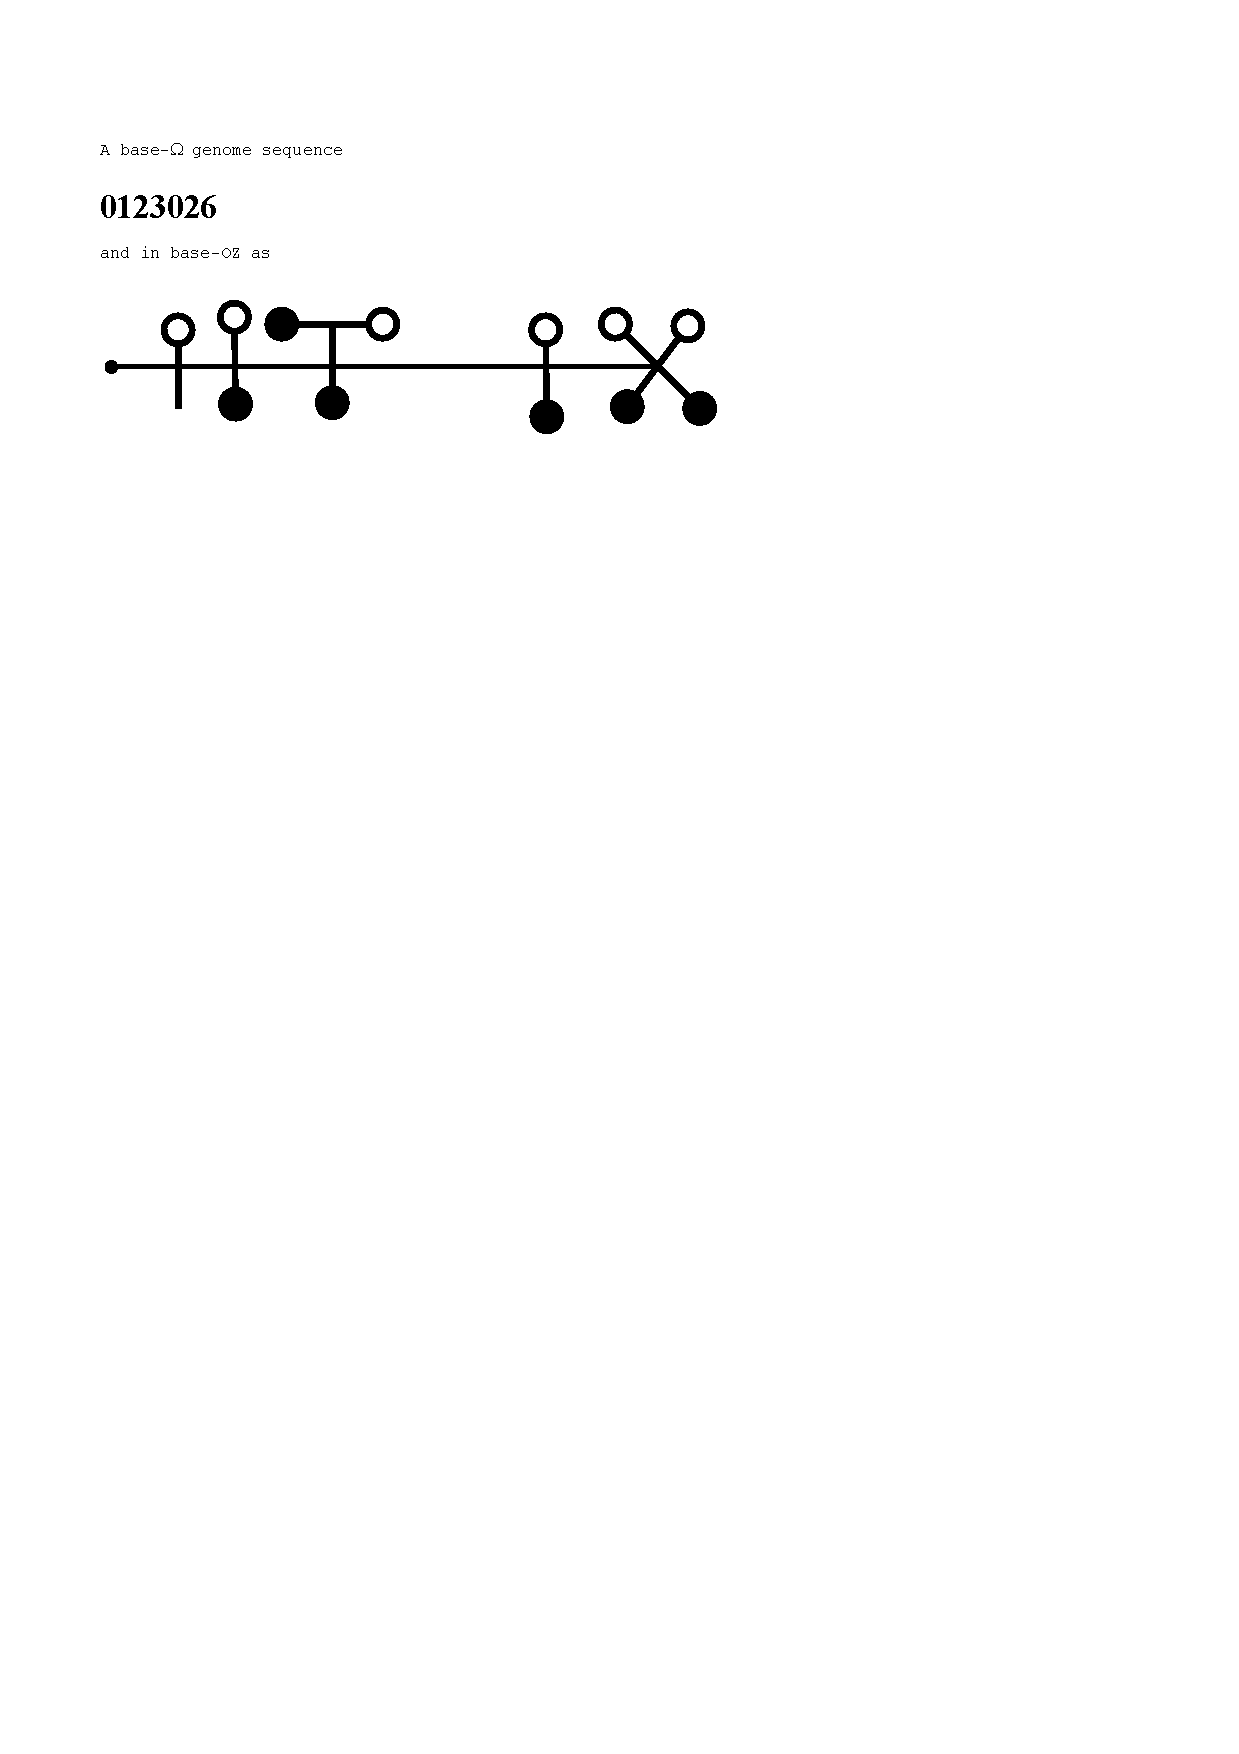
\includegraphics[trim=0cm 20cm 0cm 0cm, clip, width=0.9\textwidth,]{resources/pdfs/OZINCIPHER-APP3-EXA.pdf}\\
   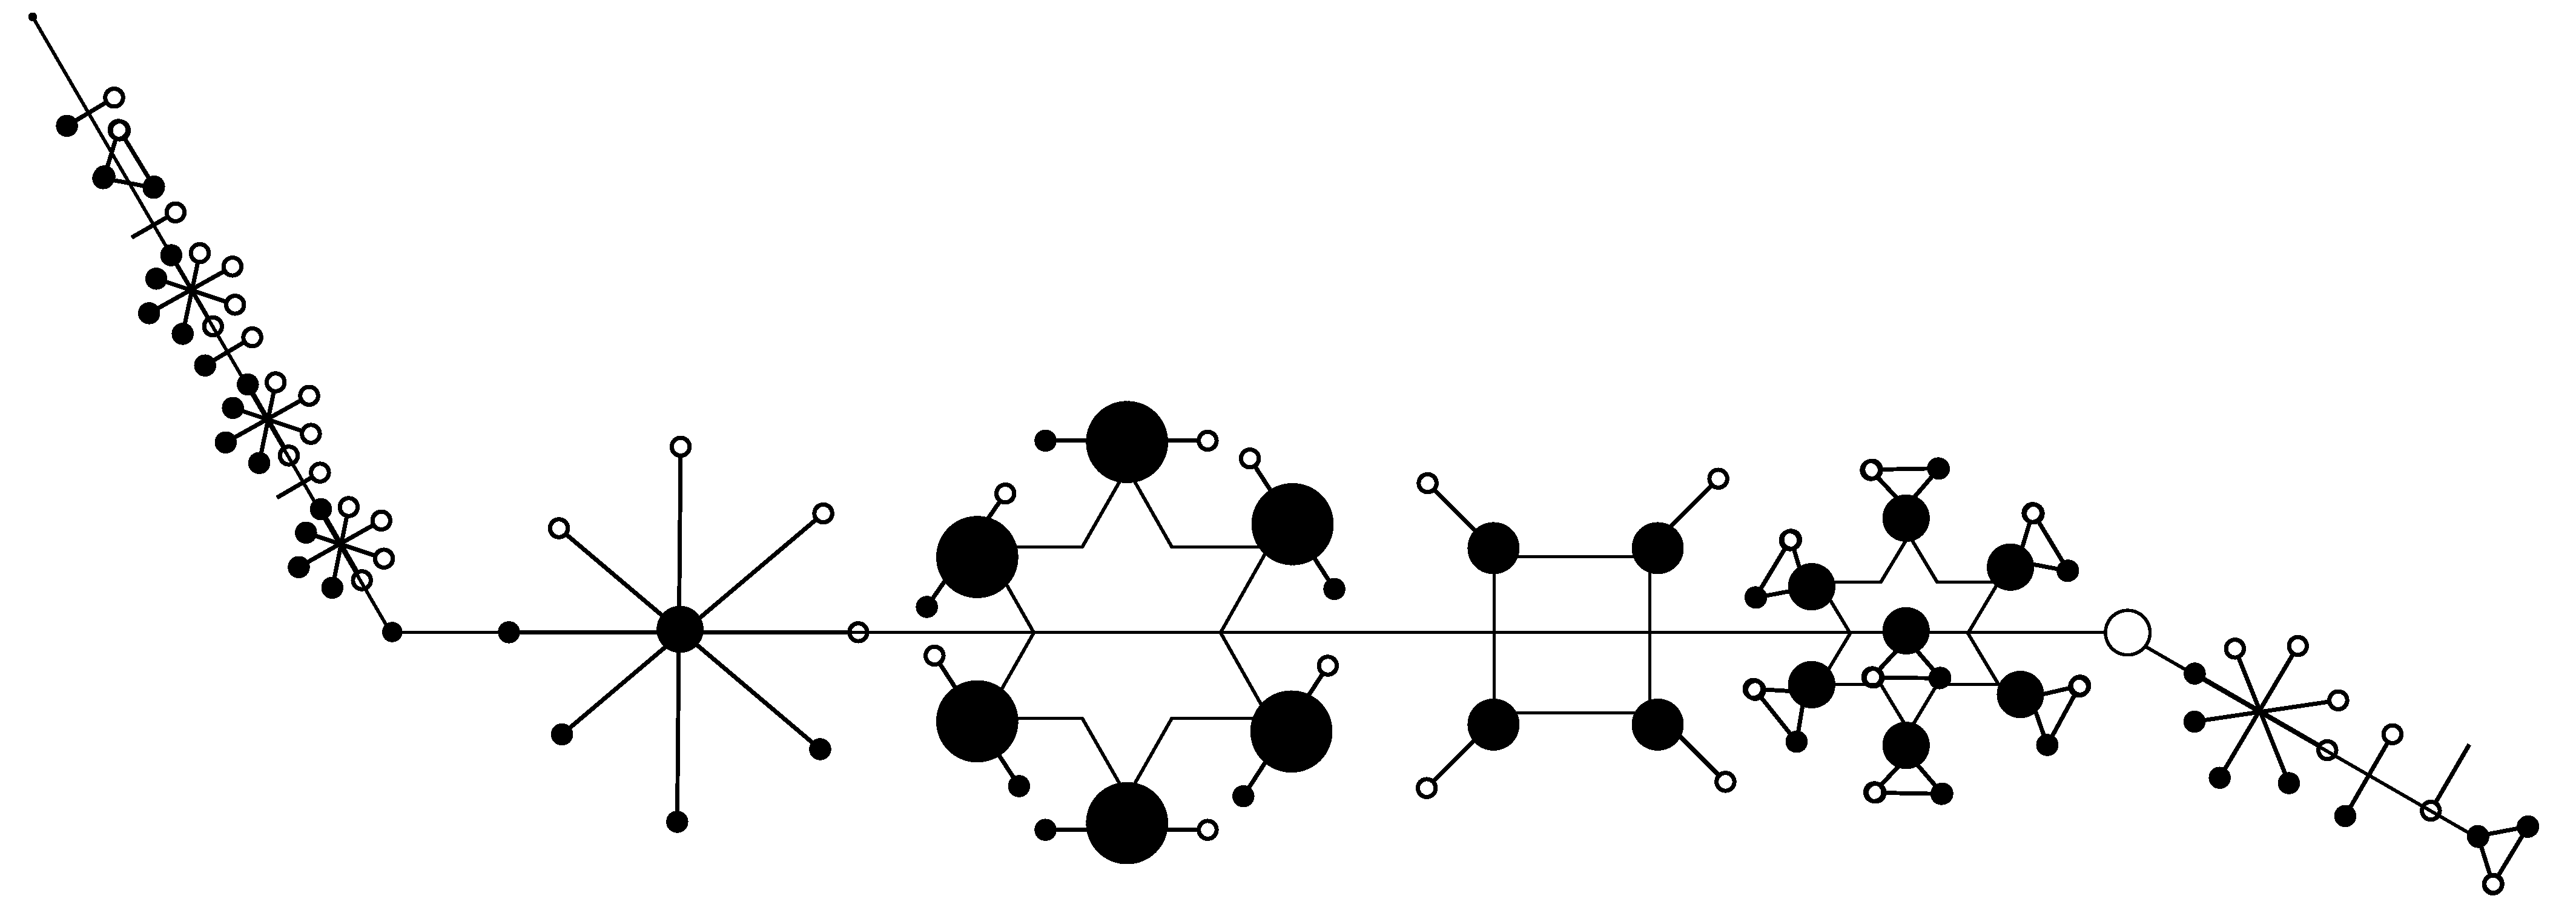
\includegraphics[trim=0cm 0cm 0cm 0cm, clip, width=0.9\textwidth,]{resources/pdfs/EXT-v2-PLATONIC-EULERVIRUS-landscape.pdf}\\
   \caption{The \textbf{x-LGES form rendering} of the $\Omega_{veuler}$, the \textbf{Euler Virus}, now with HEAD, BODY and ROOT segments.}
  \label{FIGLGESEULERVIRUSv2EXT}
  \end{center}
\end{figure}

The first example is with the notorious \textbf{Euler Virus} originally defined in \textbf{\hyperref[EQDNAV]{Equation \ref{EQDNAV}}}, and this rendering shown in \textbf{Figure \ref{FIGLGESEULERVIRUSv2EXT}} shall start to paint the new picture for you, if you compare it to the original OZIN-expression of its equivalent \textbf{mRNA} as shown in \textbf{Figure \ref{FIGOZEVIRUS}}, and then that same organism as the basic \textbf{LGES}-form in \textbf{Figure \ref{FIGLGESEULERVIRUSv2}} which shows the full genome expression minus the extension \textbf{GES} SUFFIX/ROOT.


\section{Actual DNA Sequences Expressed in the Extended Lu-Genome Expression System}

So, now that we have finished looking at what could happen with genome expression under the hypothetical LGES protocols, one might wonder, and correctly so, how might we use that system to attempt to visualize actual na-Sequences such as DNA or RNA sequences or subsequences?

Concerning working with the LGES or x-LGES as it is at the moment, the entry point barrier is that the system is defined for sequences expressed in base-10 only. That means, unless your sequence is expressed using symbols from $\psi_{10}$, there is no direct way to leverage the theory we have just presented. So, that's where we need put our attention first, with regards to processing DNA or RNA in this thought experiment.

Good enough, we have had extensive background concerning transformation of sequences across symbol sets in earlier chapters, and so, we can just re-iterate some points here.

\begin{itemize}
\item We know that any na-Sequence shall span $\psi_{na}$, which has cardinality 5 (refer to \textbf{\hyperref[LAWNA]{Law \ref{LAWNA}}}), and yet, $\invpi(\psi_{10}) = 10 > \invpi(\psi_{na})$.
\item For either DNA ($\psi_{DNA}$) or RNA ($\psi_{RNA}$), their corresponding symbol set cardinalities are just \textbf{4} and \textbf{4} respectively, which still doesn't map well to the base-10 or rather $\psi_{10}$ symbol set that the Lu-Genome Expression System requires.
\end{itemize}

So, using sequences we have already encountered, such as $\Theta_4^*$ in \textbf{\hyperref[EQ6B]{Equation \ref{EQ6B}}} --- an RNA sequence, or its original DNA form (as in \textbf{\hyperref[EQ5]{Equation \ref{EQ5}}}) how, should we go about expressing it in equivalent or sufficient $\Omega$-form?

\subsection{Converting Between Nucleic Acid Code and Numeric Codes}

First, given the constraints we have seen above, one plausible solution might be to start with a naive\footnote{I think it is naive, because, using the position-index operator $I(\omega,\Theta)$ in the encoding definition, it isn't clear how we shall ever resolve for the digit `0' given DNA has only 4 distinct symbols.} encoding that merely maps every element in $\psi_{DNA}$ to a corresponding term in $\psi_{10}$ \textbf{based not on the quantity of the symbol --- since na-Sequences aren't made of `literal numbers', but rather, based on the position of the symbol within the DNA symbol set}. So that, we have the following basic encoding-transformer:


\begin{transf}[$\psi_{DNA}$ to $\psi_{10}$ \textbf{DNA-Decimal Encoder}]
\label{TRANSFDNADECEN}
$ $\\
$\Theta \xrightarrow{O_{dna-dec-encode}(\cdot)} \Theta^*; \quad \forall \omega \in \Theta: I(\omega,\Theta) = k, \exists \rho \in \Theta^*: I(\rho,\Theta^*) = k \implies \rho = I(\omega,\psi_{DNA})$
\end{transf}


And so, using that \textbf{\hyperref[TRANSFDNADECEN]{Transformer \ref{TRANSFDNADECEN}}}, we can process any DNA sequence and map it to corresponding $\Omega$-form (or rather \textit{decimal form}) as such:

\[
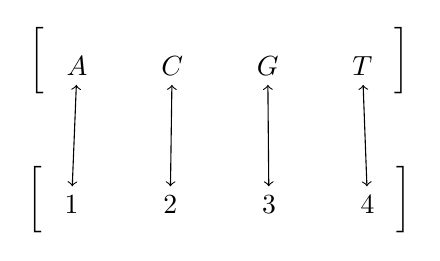
\begin{tikzpicture}[baseline=(current bounding box.center)]
  % Matrix A
  \matrix (A) [matrix of math nodes, left delimiter={[}, right delimiter={]}, row sep=1em, column sep=2em] {
    A & C & G & T \\
  };

  % Matrix B
  \matrix (B) [matrix of math nodes, left delimiter={[}, right delimiter={]}, row sep=1em, column sep=2.4em, below=3em of A] {
    1 & 2 & 3 & 4 \\
  };

  % Draw arrows from A_i to B_i
  \foreach \i in {1,2,3, 4}
    \draw[<->] (A-1-\i) -- (B-1-\i);
\end{tikzpicture}
\]


With that basic mapping, and our example DNA sequence from \textbf{\hyperref[EQ5]{Equation \ref{EQ5}}}) we see that the corresponding decimal-encoded DNA sequence shall merely be as in the following transformation:

\begin{trans}
\label{TRANSSEQATG}
$\Theta = \langle  A, T, G, A, A, A, T, T, A, T, A, G \rangle$\\
$ \xrightarrow{O_{dna-dec-encode}(\cdot)} \langle  1, 4, 3, 1, 1, 1, 4, 4, 1, 4, 1, 3 \rangle$
\end{trans}

Essentially, the symbol set for DNA sequences encoded in decimal shall only span the special symbol set we might refer to as \textbf{DNA-Digits Symbol Set}, and which we might denote as $\psi_{DD}$, and which is just:


\begin{equation}
\label{EQDNADIGSS}
\psi_{DD} = \langle 1, 2, 3, 4 \rangle
\end{equation}


So, with $\psi_{DD}$ and knowing the mapping from DNA to Decimal, we could also work backwards from decimal sequences back into DNA sequences. So, for example, assuming we took the interesting \textbf{Hi-Fi o-SSI} from \textbf{\hyperref[EQDNHIFI]{Equation \ref{EQDNHIFI}}}, and wanted to map it to an equivalent DNA sequence, we might proceed by combining the consequences of \textbf{\hyperref[THEOCOMPEQUIV]{Theorem \ref{THEOCOMPEQUIV}}} and  \textbf{\hyperref[TRANSFDNADECEN]{Transformer \ref{TRANSFDNADECEN}}}. Thus, we might start by resolving to the following approximate numerical sequence:\\


\begin{trans}
\label{EQDNHIFINUM}
$\Omega_{HiFinelle} = \langle 8,6,4,9,1,3,7,5,2,0 \rangle \rightarrow  \langle 8,6,T,9,A,G,7,5,C,0 \rangle $\\
\end{trans}




However, as warned earlier on, transformations via \textbf{\hyperref[TRANSFDNADECEN]{Transformer \ref{TRANSFDNADECEN}}} would be somewhat \textit{weak} when dealing with the reverse case --- decimal-to-DNA decoding, especially because not all symbols in $\psi_{10}$ shall have meaningful equivalent terms in $\psi_{DNA}$. So, better we start by solving that problem instead.

Thus, with some \textit{necessary tweak} --- that, instead of mapping from $\psi_{DNA}$ to $\psi_{10}$ and vice-versa, we take $\psi_{na}$ which has exactly 5 elements and which is a superset of $\psi_{DNA}$\footnote{Refer to \textbf{\hyperref[DEFNASEQ]{Definition \ref{DEFNASEQ}}}}, and then map any symbol from $\psi_{na}$ to $\psi_{10}$ and vice-versa as per the following non-trivial transformer:


\begin{center}
\fbox{
\begin{minipage}{\textwidth}
\begin{transf}[$\psi_{na}$ to $\psi_{10}$ \textbf{na-to-Decimal Decoder}]
\label{TRANSFDECTONASEQ}
$ $\\
$\Theta \xrightarrow{O_{na-dec-decode}(\cdot)} \Theta^*;$\\
$\forall \omega_i \in \psi_{na}: I(\omega_i,\psi_{na}) = i \implies \exists d_j \in \psi_{10}: I(d_j,\psi_{10}) = j = i \quad \lor \quad I(d_j,\psi_{10}) = \invpi(\psi_{na}) + i \quad \implies \omega_i \leftrightarrow d_j $\\
$\land \quad \forall \alpha_k \in \Theta \quad \exists d_k \in \Theta^*: I(\alpha_k,\Theta) = I(d_k,\Theta^*) = k \quad \land \quad I(d_k,\psi_{10}) = I(\alpha_k,\psi_{na}) \lor I(d_k,\psi_{10}) = \invpi(\psi_{na}) + I(\alpha_k,\psi_{na}) \quad \implies \alpha_k \leftrightarrow d_k $
$\qed$\\
\end{transf}
\end{minipage}}
\\
\end{center}




So that, by \textbf{\hyperref[TRANSFDECTONASEQ]{Transformer \ref{TRANSFDECTONASEQ}}}, we arrive at complete decimal-to-DNA and decimal-to-RNA or generally decimal-to-na-Sequence symbol encoding-decoding is as shown in the following diagram:


\[
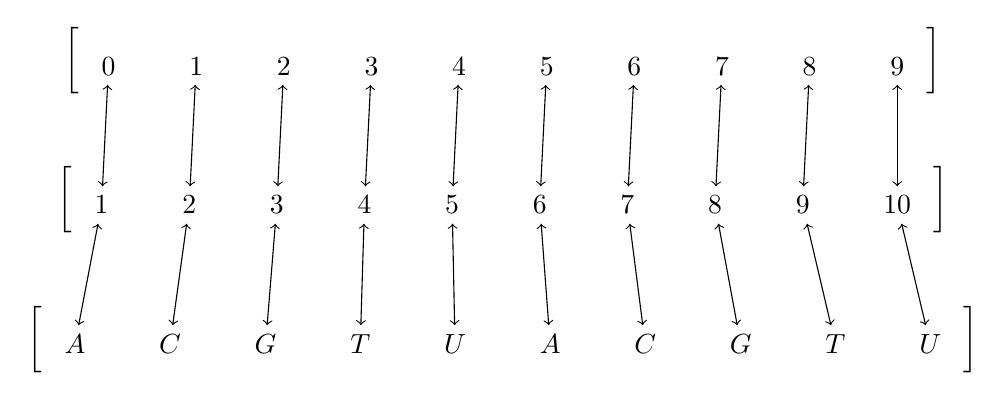
\begin{tikzpicture}[baseline=(current bounding box.center)]
  % Matrix A
  \matrix (A) [matrix of math nodes, left delimiter={[}, right delimiter={]}, row sep=1em, column sep=2em] {
    0 & 1 & 2 & 3 & 4 & 5 & 6 & 7 & 8 & 9\\
  };

  % Matrix B
  \matrix (B) [matrix of math nodes, left delimiter={[}, right delimiter={]}, row sep=1em, column sep=2em, below=3em of A] {
    1 & 2 & 3 & 4 & 5 & 6 & 7 & 8 & 9 & 10\\
  };
  
   % Matrix C
  \matrix (C) [matrix of math nodes, left delimiter={[}, right delimiter={]}, row sep=1em, column sep=2em, below=3em of B] {
    A & C & G & T & U & A & C & G & T & U\\
  };

  % Draw arrows from A_i to B_i
  \foreach \i in {1,2,3,4,5,6,7,8,9,10}
    \draw[<->] (A-1-\i) -- (B-1-\i);
    
  % Draw arrows from B_i to C_i
  \foreach \i in {1,2,3,4,5,6,7,8,9,10}
    \draw[<->] (B-1-\i) -- (C-1-\i);
\end{tikzpicture}
\]

Of course, the necessary tweak here, especially for target sequences specific to either DNA or RNA and not both, the tricky terms `T' and `U' need to be dealt with as necessary --- possibly with a basic swapping of all `U' with `T' for an na-Sequence targeting a DNA processor, and vice-versa for those targeting strict RNA processors. 

Also, that mapping offers us a basic protraction na-Sequence that is a basic multiplication of the $\psi_{na}$ symbol set by 2. Because it maps nicely to terms in $\psi_{10}$, both sequences having equal length, we could use it in various problems such as in generating random na-Sequences or mapping random base-10 o-SSI sequences to corresponding na-Sequences --- or virtually any decimal sequence of any length. 

That said, let us set that special sequence aside for later use in the following equation:

\begin{equation}
\label{EQDUPLNASEQ}
\Theta_{2na} =  = \psi_{na} \cdot \psi_{na} = \langle A , C , G , T , U , A , C , G , T , U \rangle
\end{equation}\\

However, and also related, we might, also come to appreciate a related sequence, $\Theta_{palna}$ that is a palindrome derived from $\psi_{na}$, and definitely, with the same length as $\psi_{10}$.


\begin{equation}
\label{EQPALNASEQ}
\Theta_{palna} = \psi_{na} \cdot \lnot(\psi_{na}) =  \langle A , C , G , T , U , U , T , G , C , A \rangle
\end{equation}\\


That said, and back to our \textbf{x-LGES} problem...

\subsection{Revisiting Numeric Sequences}

Before we proceed with actual na-Sequences, we shall first revisit hypothetical genome sequences expressed in numeric form, and then shall use the experience we garner to handle processing of actual na-Sequences later.

So, returning to that interesting \textbf{Hi-Fi o-SSI} sequence --- $\Omega_{HiFinelle} = 8649137520$, only partially translated into DNA-code in  \textbf{\hyperref[EQDNHIFINUM]{Transformation \ref{EQDNHIFINUM}}}, if we are to convert it to an equivalent na-Sequence using the new information we have, we would obtain the results:

\begin{trans}
\label{EQDNHIFINUMCOMPLETE}
$\Omega_{HiFinelle} = \langle 8,6,4,9,1,3,7,5,2,0 \rangle \xrightarrow{O_{na-dec-decode}(\cdot)}$\\
$  \langle T,C,U,U,C,T,G,A,G,A \rangle = TCUUCTGAGA$\\
\end{trans}


Which, if we wish to constrain it to just the DNA symbol set, would be as:


\begin{trans}
$\Omega_{HiFinelle} = 8649137520 \xrightarrow{O_{na-dec-decode}(\cdot)} TCUUCTGAGA$\\
$ \quad  \xrightarrow{O_{mRNA-encode}(\cdot)} UCUUCUGAGA \quad  \xrightarrow{O_{DNA-encode}(\cdot)} TCTTCTGAGA$
\end{trans}


And that last transformation was made possible by chaining several transformers, some of which we have already encountered in earlier discussions, so that the final sequence is strictly DNA-encoded. Thus, our $\Omega_{HiFinelle}$ can be mapped from base-$\Omega$ into base-DNA and vice-versa as we have seen. These ideas can definitely then be used to process any other numeric sequence when there is need to map it to or treat is as a legitimate na-Sequence.

However, for the case of our gene expression system, we really don't care or need the na-Sequence expressions to begin with. And so, given we already have the numeral equivalent of $\Omega_{HiFinelle}$, we can directly advance to rendering the organism that might ensue from processing it via \textbf{x-LGES}. Note that, for this particular sequence, we had already dealt with its \textbf{IFA} prefix encoded in base-OZIN --- see \textbf{\hyperref[FIGOZHIFI]{Figure \ref{FIGOZHIFI}}}. Thus, proceeding via a meaningful \textbf{transformatic-distillation} such as we did for the Euler Virus in \textbf{\hyperref[TRANSGENSEQEVIRUS]{Transformation \ref{TRANSGENSEQEVIRUS}}}\\


\begin{trans}
\label{TRANSGENSEQHiFinelle}
$\Omega_{HiFinelle} = \langle 8,6,4,9,1,3,7,5,2,0 \rangle \rightarrow$\\
$ \hbar(\overset{>}{\Omega_{HiFinelle}}) = \text{\textbf{8}1\textbf{6}1\textbf{4}1\textbf{9}1\textbf{1}1\textbf{3}1\textbf{7}1\textbf{5}1\textbf{2}1\textbf{0}1} \rightarrow \overset{>}{\Omega_{HiFinelle}} = \langle 8,6,4,9,1,3,7,5,2,0 \rangle$\\
$\implies  m = \invpi(\overset{>}{\Omega_{HiFinelle}}) = 10 \implies  \boxed{\psi_{pf}}_{10} = \langle 6, 3, 8, 2, 1, 9, 7, 4, 0, 5 \rangle$\\
$\implies \boxed{OZ(\Omega_{HiFinelle})} = \langle 6_{pf} \otimes 8_{oz},  3_{pf} \otimes 6_{oz}, 8_{pf} \otimes 4_{oz}, 2_{pf} \otimes 9_{oz}, 1_{pf} \otimes 1_{oz}, 9_{pf} \otimes 3_{oz}, 7_{pf} \otimes 7_{oz}, 4_{pf} \otimes 5_{oz}, 0_{pf} \otimes 2_{oz}, 5_{pf} \otimes 0_{oz} \rangle$\\
$\implies \boxed{OZ(\Omega_{HiFinelle})}^* = \langle  8,6,4,9,1,3,7,5,2,0 \rangle_{oz} \cdot \langle 6_{pf} \otimes 8_{oz},  3_{pf} \otimes 6_{oz}, 8_{pf} \otimes 4_{oz}, 2_{pf} \otimes 9_{oz}, 1_{pf} \otimes 1_{oz}, 9_{pf} \otimes 3_{oz}, 7_{pf} \otimes 7_{oz}, 4_{pf} \otimes 5_{oz}, 0_{pf} \otimes 2_{oz}, 5_{pf} \otimes 0_{oz} \rangle \cdot \langle  8,6,4,9,1,3,7,5,2,0 \rangle_{oz}$

\end{trans}


Without actually wasting time and space rendering the visual equivalence of that organism, among interesting things to note from \textbf{Transformation \ref{TRANSGENSEQHiFinelle}} is that unlike in \textbf{\hyperref[TRANSGENSEQEVIRUS]{Transformation \ref{TRANSGENSEQEVIRUS}}}, we have applied the extended LGES algorithm --- \textbf{\hyperref[ALGCOZINPLATOEXT]{Algorithm \ref{ALGCOZINPLATOEXT}}}, so that the final expression in that transformation contains the HEAD, BODY and ROOT of the organism. Also, and interesting to note, that despite this particular sequence having no exciting \textbf{IFA MSS} --- since all the symbols in the original sequence have frequency 1 (which is why we see the organism's HEAD and ROOT looking exactly the same\footnote{I won't show many pictures here except perhaps \textbf{Figure \ref{FIGEARTHWORM}}, but some kinds of \textbf{millipedes} and \textbf{centipedes} have this strange symmetrical anatomy that makes it difficult to distinguish its head from the tail. Earthworms too! Someone suggested the concept of the \textit{Ouroboros} from esoteric folklore, that exhibits a kind of self-referential form, however, in my local folklore and vocabulary, we have a peculiar snake-like creature known as \textit{namunungu} that exhibits this peculiar form too.} \textit{in numeric form}), though, because of the consequences of how the BODY component is generated, we see a potential mid-BODY-JOINT --- \textbf{PFA} node $0_{pf} \otimes 2_{oz}$, that would definitely make the corresponding \textbf{FGE} interesting to look at. Also, given $0_{oz}$ maps to ``STOP/GAP", the final term in the \textbf{PFA}, $5_{pf} \otimes 0_{oz}$, would potentially look something like \textbf{a hand} perhaps --- it is a geometric structure of exactly 5 vertices (just like on a human palm), and like it, with \textit{discontinuities} at the appendage points/vertices\footnote{Jokes aside, normally in esoterica, \textit{magical wands} are depicted as being a rod that terminates in a 5-vertex shape --- typically a pentagram, so a creative mind might start to think of the $\Omega_{HiFinelle}$ creature as a potentially \texttt{magical creature}!}. 


\begin{figure}[H]
  \begin{center}
  %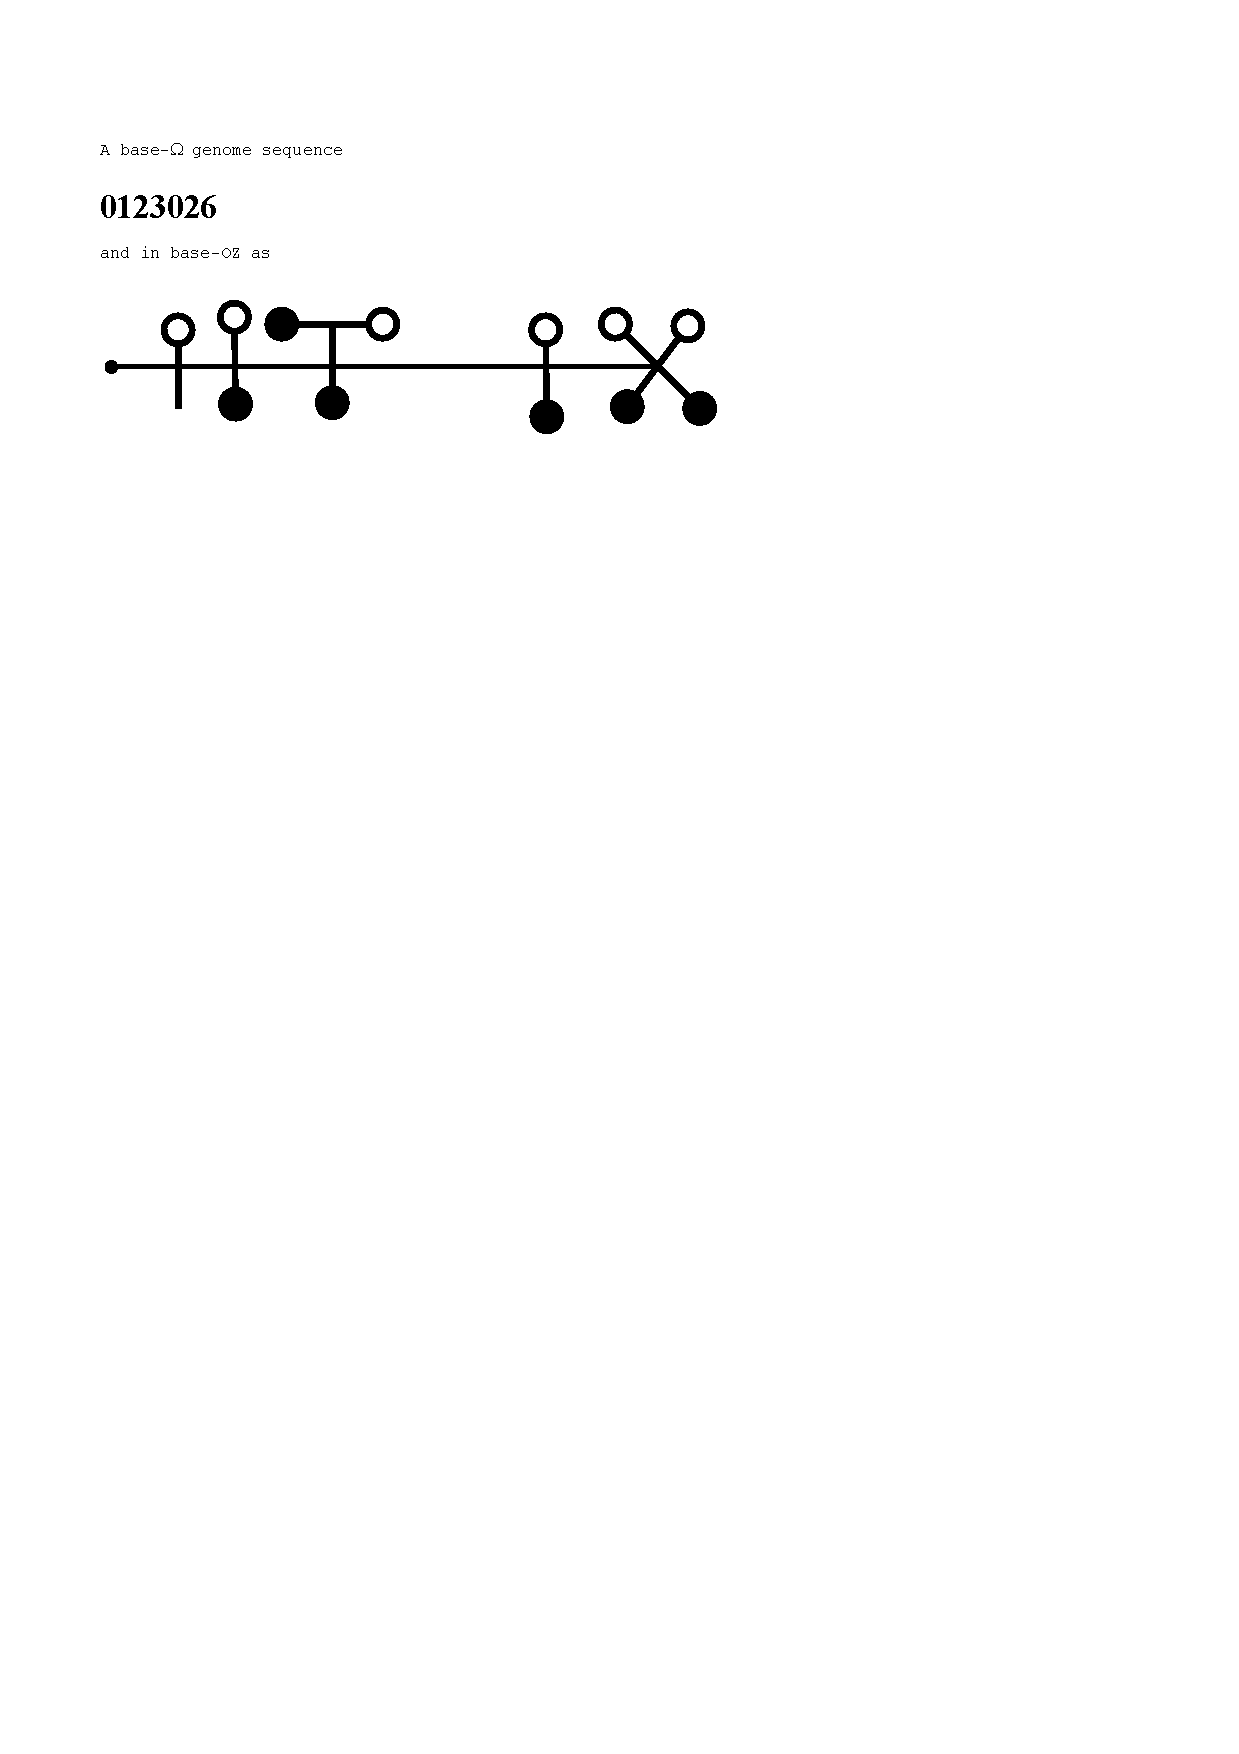
\includegraphics[trim=0cm 20cm 0cm 0cm, clip, width=0.9\textwidth,]{resources/pdfs/OZINCIPHER-APP3-EXA.pdf}\\
   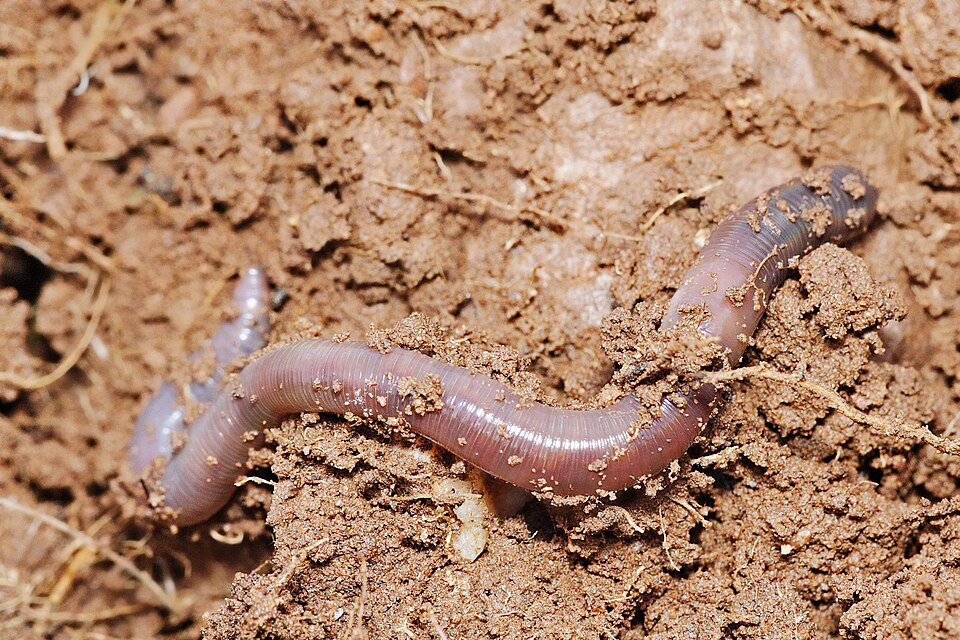
\includegraphics[trim=0cm 0cm 0cm 0cm, clip, width=0.9\textwidth,]{resources/images/Earthworm.jpg}\\
   \caption{An example of an actual organism from nature --- an Earthworm, for which, like the x-LGES rendering of the sequence $\Omega_{HiFinelle}$, results in a genome expression for a creature that almost looks the same at the HEAD and ROOT. Image sourced from Wikimedia Commons\cite{earthwormImage}.}
  \label{FIGEARTHWORM}
  \end{center}
\end{figure}





\subsection{x-LGES applied to named DNA Sequences}

Now that we have attained sufficient experience with expressing pure numeric sequences, we can return to actual na-Sequences, and checkout some potentially enlightening scenarios.

First, we shall want to have a way to assign meaningful names to our sequences. For example, the sequence from \textbf{\hyperref[TRANSSEQATG]{Transformation \ref{TRANSSEQATG}}}. Instead of just calling it $\Theta$, we could adapt a name from its corresponding na-Sequence, and then use that to distinguish it from other na-Sequences we shall want to compare it against.

Without caring whether it actually has a standard or conventional name based on its actual na-composition as depicted, we could adopt a system such as picking the first letters of its contained codons in the order they appear in the sequence, and then assign it a name based on the resulting acronym. So, we for example know from \textbf{\hyperref[TAB1]{Table \ref{TAB1}}} originally associated with that sequence, that the corresponding codons  by the code-names (also see \textbf{\hyperref[EQ4]{Equation \ref{EQ4}}}) are as follows:

\begin{equation}
\Theta = \langle Met, Lys, Leu, Amber \rangle
\end{equation}\\

So that we can just obtain a name for the sequence using the above suggested strategy as such:

\begin{trans}
$\langle Met, Lys, Leu, Amber \rangle \rightarrow \langle M, L, L, A \rangle \rightarrow MLLA$
\end{trans}

Thus, we might formally refer to our gene-program with a proper name as $\Theta_{MLLA}$ or just the \textbf{MLLA}-gene program --- where no confusion might arise, we shall just refer to it as $\Theta_{ml}$. 

So, how would this program's corresponding sequence appear if it were expressed in the x-LGES?

We have its corresponding $\Omega$-form expression in \textbf{\hyperref[TRANSSEQATG]{Transformation \ref{TRANSSEQATG}}}, so that:\\

\begin{equation}
\label{EQSEQMLLA}
\Theta_{ml} = \langle  1, 4, 3, 1, 1, 1, 4, 4, 1, 4, 1, 3 \rangle
\end{equation}\\

From that, we can leverage the pre-rendering calculus we have already encountered, well-applied in \textbf{\hyperref[TRANSGENSEQHiFinelle]{Transformation \ref{TRANSGENSEQHiFinelle}}}, and so that we can then readily apply \textbf{\hyperref[ALGCOZINPLATOEXT]{Algorithm \ref{ALGCOZINPLATOEXT}}} to $\Theta_{ml}$. The necessary derivation of the corresponding genome expression shall be as in: 


\begin{center}
\fbox{
\begin{minipage}{\textwidth}


\begin{trans}
\label{TRANSGENSEQMLLA}
$\Theta_{ml} = \langle 1, 4, 3, 1, 1, 1, 4, 4, 1, 4, 1, 3 \rangle \rightarrow \hbar(\overset{>}{\Theta_{ml}}) = \text{\textbf{1}6\textbf{4}4\textbf{3}2} \rightarrow \overset{>}{\Theta_{ml}} = \langle 1,4,3 \rangle \implies  m = \invpi(\overset{>}{\Theta_{ml}}) = 3 \implies  \boxed{\psi_{pf}}_{3} = \langle 7, 5, 3 \rangle$\\
$\implies \boxed{OZ(\Theta_{ml})} = \langle 7_{pf} \otimes 1_{oz},  5_{pf} \otimes 4_{oz}, 3_{pf} \otimes 3_{oz}\rangle$\\
$\implies \boxed{OZ(\Theta_{ml})}^* = \langle 1, 4, 3, 1, 1, 1, 4, 4, 1, 4, 1, 3 \rangle_{oz} \cdot \langle 7_{pf} \otimes 1_{oz},  5_{pf} \otimes 4_{oz}, 3_{pf} \otimes 3_{oz} \rangle \cdot \langle  1,4,3 \rangle_{oz}$
\end{trans}


\end{minipage}}
\\
\end{center}

The corresponding fully rendered \textbf{FGE} would be as depicted below:

\begin{figure}[H]
  \begin{center}
  %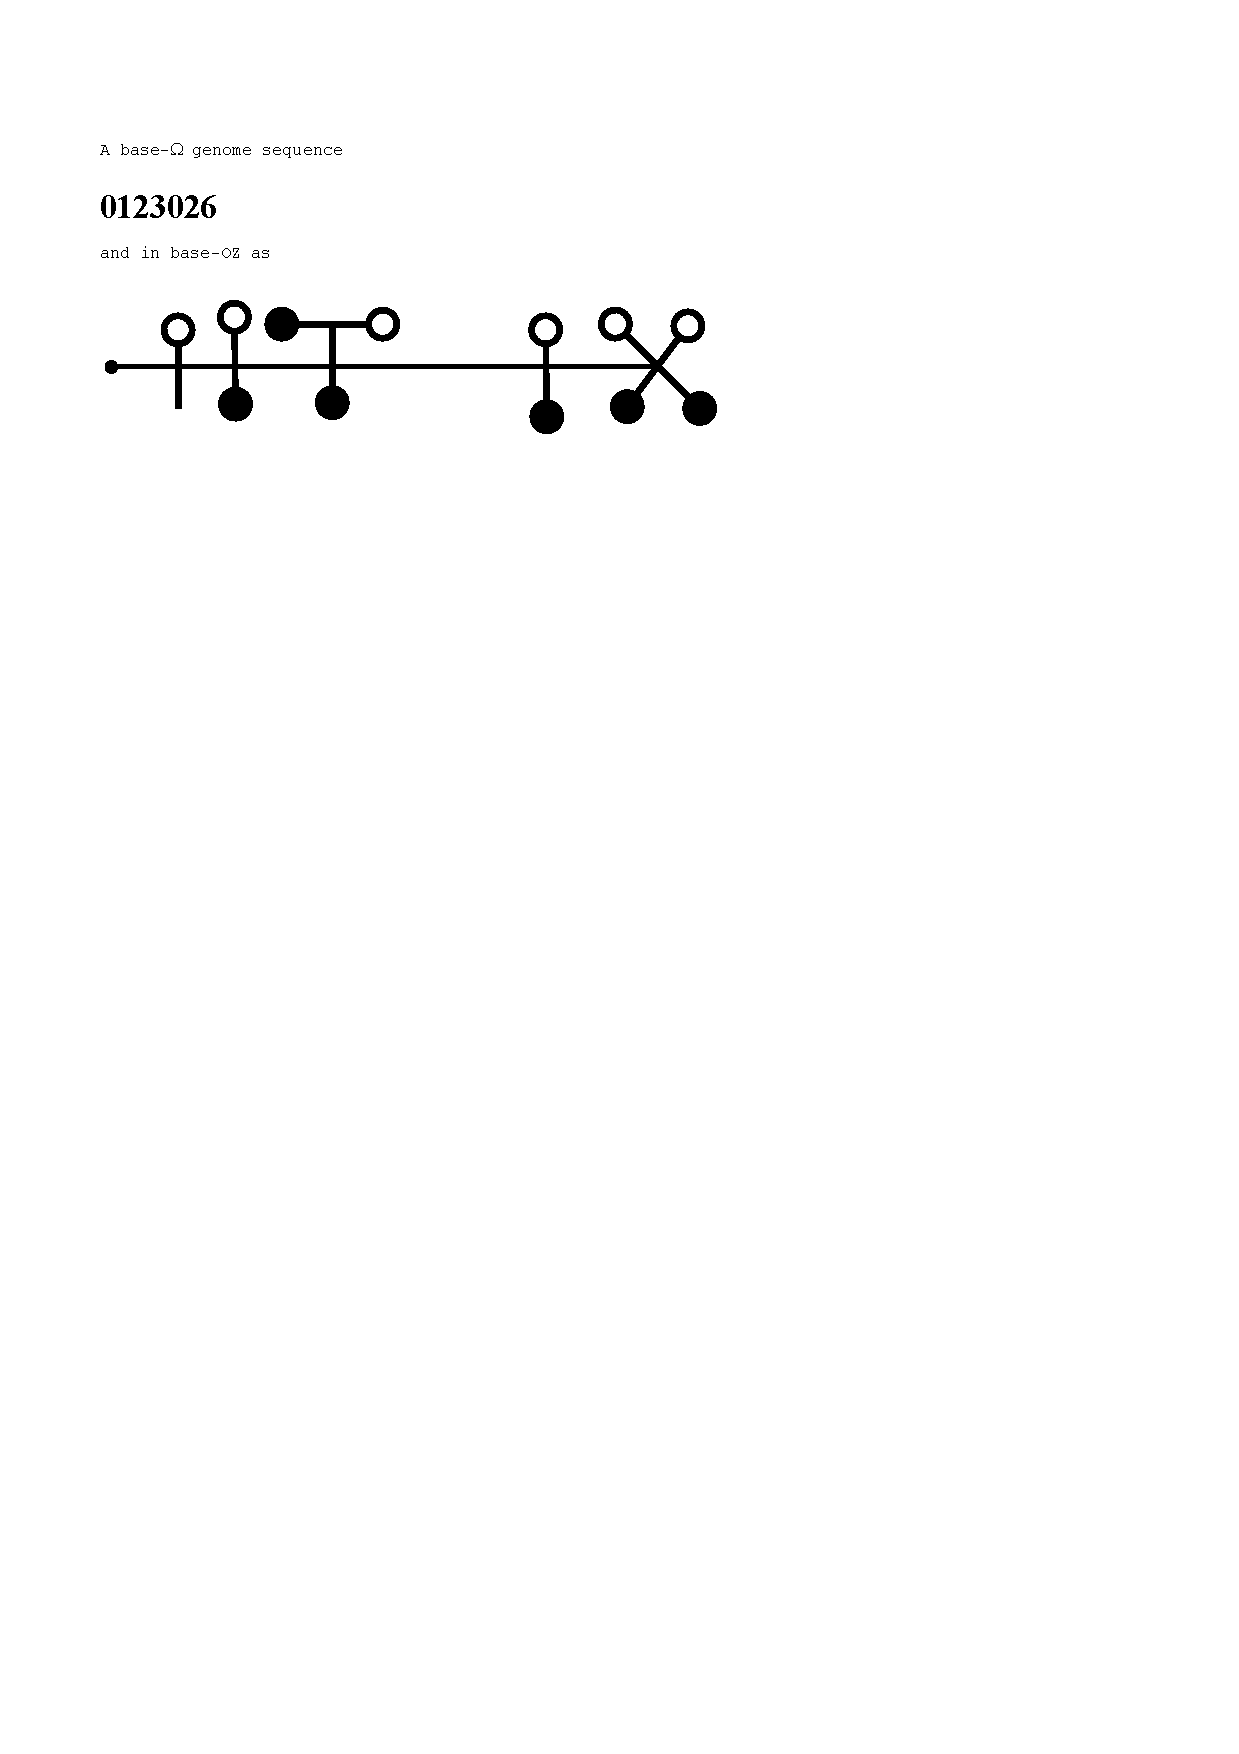
\includegraphics[trim=0cm 20cm 0cm 0cm, clip, width=0.9\textwidth,]{resources/pdfs/OZINCIPHER-APP3-EXA.pdf}\\
   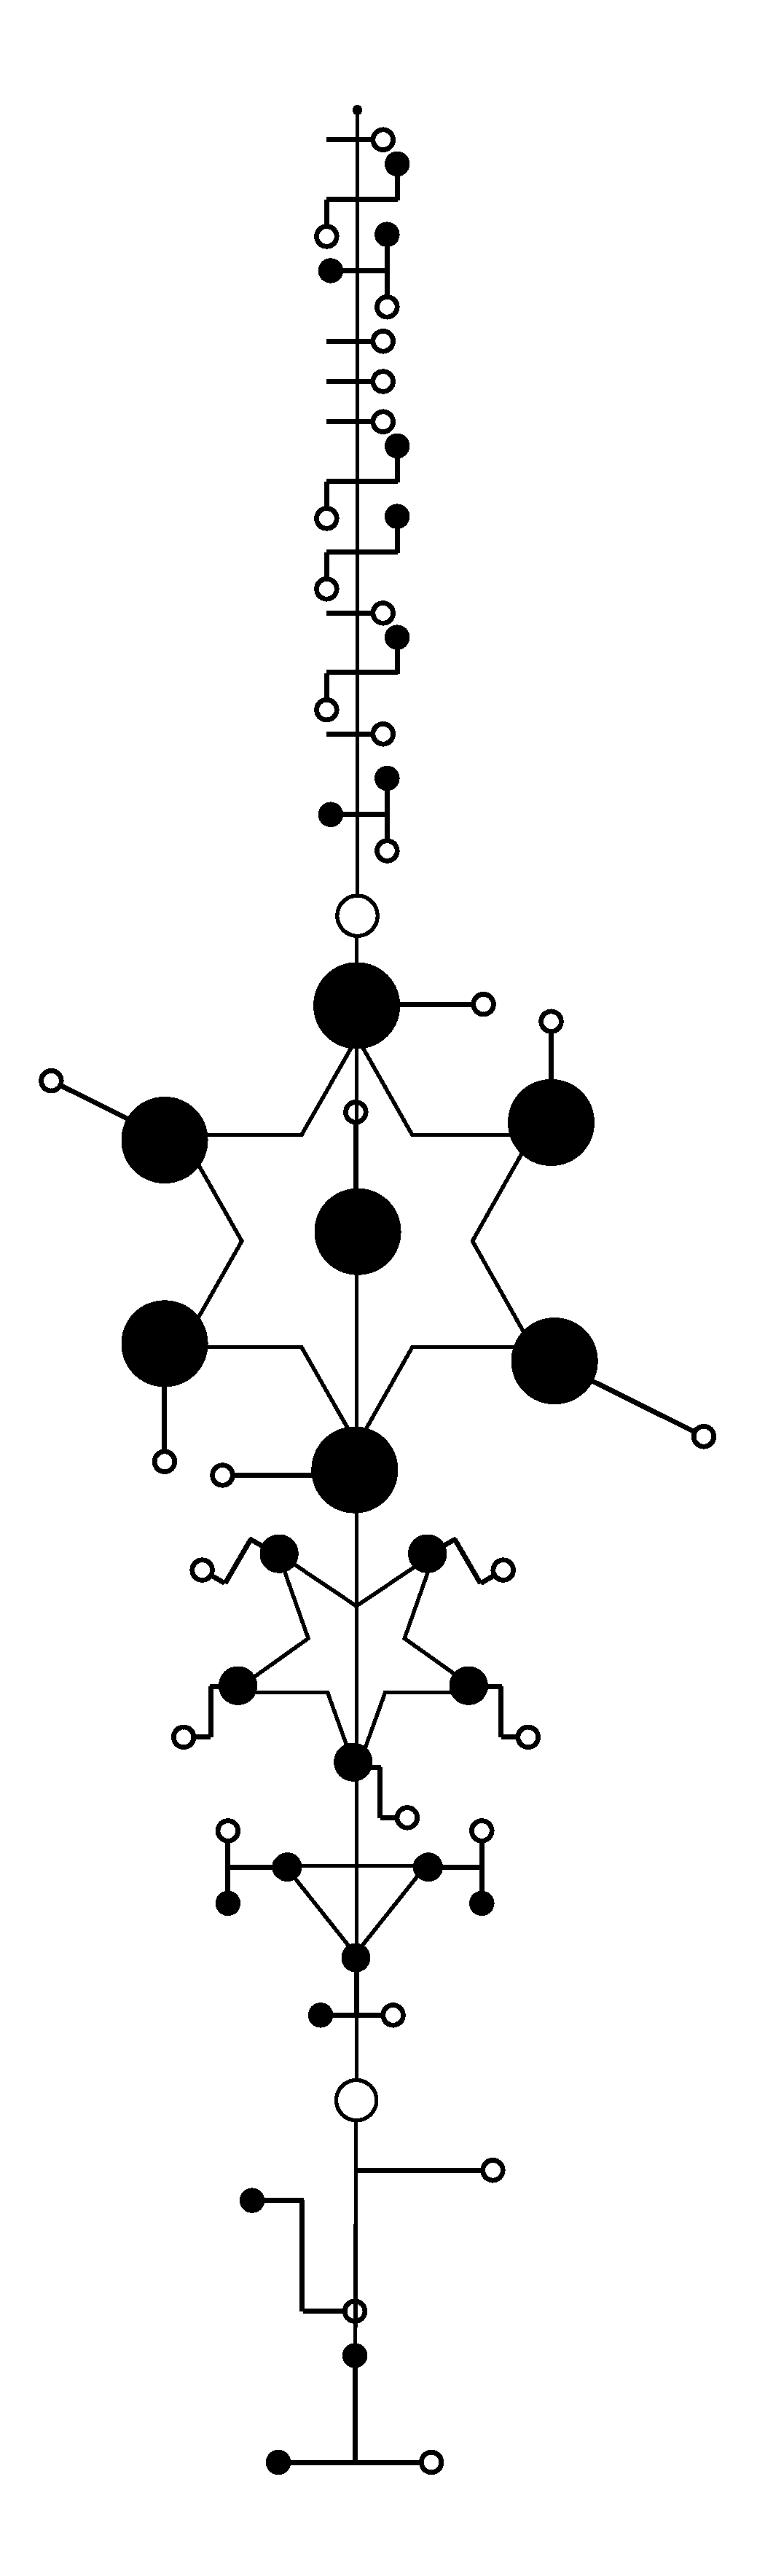
\includegraphics[trim=0cm 0cm 0cm 0cm, clip, height=0.9\textheight,]{resources/pdfs/xLGES-PLATONIC-MLLA-landscape.pdf}\\
   \caption{The \textbf{x-LGES form rendering} of the sequence $\Theta_{mlla}$, depicting its complete \textbf{FGE} with HEAD, BODY and ROOT segments.}
  \label{FIGLGESMLLA}
  \end{center}
\end{figure}


Thus we conclude our treatment of TRANSFORMATICS in GENETICS.


\chapter{Conclusion}
\label{CONC}

In this work, we have advanced our knowledge concerning the important and fundamental subject of genetics with new theory and practical ideas previously only held informally or totally unknown. We have explored several interesting ways by which the newly proposed mathematical field of inquiry, known as \textbf{TRANSFORMATICS} --- potentially a sub-field of/fusion of mathematical statistics and linear algebra\footnote{As in the conclusion of the original transformatics paper\cite{transformatics}, the author strongly feels that in the future, and with further investments in research, development of theory and applications, transformatics might become its own sub-field of mathematics, distinct from both statistics and linear algebra.}, might be applied in the sub-field of the biological sciences known as \textbf{GENETICS}. 

Though much of the work was mathematical in nature, we have also had lots of useful theory proposed in the form of conceptual and especially philosophical ideas relating to how to understand or leverage genetics through the lens of a sequence analyst and/or a computer scientist. 

In terms of concrete \textbf{Key Metrics and Contributions} this single work has brought to surface:
\begin{enumerate}
\item{ \textbf{11 Working Definitions} were developed in relation to various concepts in analytical genetics, sequence analysis and sequence processing in general, and these include:

	\begin{enumerate}
	\item The \textbf{na-Sequences} --- see  \textbf{\hyperref[DEFNASEQ]{Definition \ref{DEFNASEQ}}}
	\item The \textbf{START-Codons} --- see \textbf{\hyperref[DEFSTARTCOD]{Definition \ref{DEFSTARTCOD}}}
		\item The \textbf{STOP-Codons} --- see \textbf{\hyperref[DEFSTOPCOD]{Definition \ref{DEFSTOPCOD}}}
	\item The \textbf{Sequence Characteristic} --- see  \textbf{\hyperref[DEFSEQCHAR]{Definition \ref{DEFSEQCHAR}}}
	\item The \textbf{Population Characteristic} --- see  \textbf{\hyperref[DEFPOPCHAR]{Definition \ref{DEFPOPCHAR}}}
	\item The \textbf{Genome Sequencer} --- see  \textbf{\hyperref[DEFGENOMESEQ]{Definition \ref{DEFGENOMESEQ}}}
	\item The \textbf{Ribosome} --- see  \textbf{\hyperref[DEFRIBOSOME]{Definition \ref{DEFRIBOSOME}}}
	\end{enumerate}

}
\item{ \textbf{4 Theorems} were developed and presented for the first time, spanning genetic sequences and then sequence complements in general. These include...

	\begin{enumerate}
	\item \textbf{Complement Sequences} --- see  \textbf{\hyperref[THEOCOMPLEMENTS]{Theorem \ref{THEOCOMPLEMENTS}}}
	\item \textbf{Complement of an o-SSI is an o-SSI} --- see  \textbf{\hyperref[THEOCOMPLOSSI]{Theorem \ref{THEOCOMPLOSSI}}} 
	\item \textbf{Equivalence of Sequences} under the Complement Transform  --- see  \textbf{\hyperref[THEOCOMPEQUIV]{Theorem \ref{THEOCOMPEQUIV}}} 
	\end{enumerate}
}
\item {\textbf{3 Laws} were distilled and presented for the first time:
	\begin{enumerate}
	\item \textbf{\hyperref[LAWNA]{Law \ref{LAWNA}}}: Concerning the nucleic acid identifier symbol set, $\psi_{na}$. 
	\item \textbf{\hyperref[LAW2]{Law \ref{LAW2}}}: Concerning Introns: Non-coding gene-programs.
	\item \textbf{\hyperref[LAWGDL]{Law \ref{LAWGDL}}}: The \textbf{Identity Genome Sequence} Law.
	\end{enumerate}
}
\item{ \textbf{15 Transformers} were developed and presented for the first time, including...

	\begin{enumerate}
	\item The formal definition of the \textbf{Ribosome} as a \textbf{Protein Generator} (\textbf{\hyperref[TRANSF3]{Transformer \ref{TRANSF3}}})
	\item The \textbf{n-Gram Generator} (\textbf{\hyperref[TRANSFBUND]{Transformer \ref{TRANSFBUND}}})
	\item The \textbf{Sequence Look-up System} that leverages G$\ddot{o}$del numbers for efficient DNA-database queries (\textbf{\hyperref[TRANSFSEQLOOKUP]{Transformer \ref{TRANSFSEQLOOKUP}}})
	\item The \textbf{Random Sequence/Symbol Generator} that can construct random DNA/RNA sequences, but also any arbitrary random\footnote{We could have wanted to generalize this generator so that it can also handle the case of non-random sequence generation --- especially since it already bases its generated sequence on the properties of some input sequence, so that for example we can generate sequences that reflect the symbol distribution within the input/sample sequence (something akin to how a ChatGPT model can generate new text based on/related to some samples with say non-uniform symbol distributions), but we chose to not do that within the context of this present work, and shall leave that for a future publication and treatment.} sequence (\textbf{\hyperref[TRANSFRSG]{Transformer \ref{TRANSFRSG}}})
	\item A transformer for converting between pure numbers (in base-10) into DNA/RNA code, and vice-versa --- the $\psi_{na}$ to $\psi_{10}$ \textbf{na-to-Decimal Decoder} (\textbf{\hyperref[TRANSFDECTONASEQ]{Transformer \ref{TRANSFDECTONASEQ}}})
	\end{enumerate}
	
	and many more big and/or small, but essential transformer utilities and specifications.

}
\item{ \textbf{28 Transformations} were presented to help advance generic as well as particular computational solutions to many kinds of basic problems in sequence analysis, processing and several concerning gene/genome expression problems, including some special ones such as:

	\begin{itemize}
	\item \textbf{\hyperref[TRANSGENSEQ]{Transformation \ref{TRANSGENSEQ}}} that generalizes the intricate process of generating a correct \textbf{consensus genome sequence} via \textbf{genome sequencing}.
	\item \textbf{\hyperref[TRANSGENSEQHiFinelle]{Transformation \ref{TRANSGENSEQHiFinelle}}} that serves as a good template for the intricate process underlying the \textbf{derivation of a Full Genome Expression} from a plain sequence using the \textbf{x-LGES}.
	\end{itemize}

 
 }
\item{\textbf{8 Algorithms} were developed and presented for the first time, including:
	\begin{enumerate}
	\item \textbf{\hyperref[ALGCSA]{Algorithm \ref{ALGCSA}}}: The \textbf{Closest Sequence Algorithm}.
	\item \textbf{\hyperref[ALGtMCS]{Algorithm \ref{ALGtMCS}}}: The \textbf{tMCS} Algorithm for computing the Maximum Common Subsequence.
		\item \textbf{\hyperref[ALGLUSHUFFLEA]{Algorithm \ref{ALGLUSHUFFLEA}}}: The \textbf{First Lu-Shuffle Algorithm} (FLSA): $\text{lu\_shuffler\_a}(\Theta, k)$.
	\item \textbf{\hyperref[ALGLUSHUFFLEB]{Algorithm \ref{ALGLUSHUFFLEB}}}: The \textbf{Second Lu-Shuffle Algorithm} (SLSA): $\text{lu\_shuffler\_b}(\Theta, k)$.
	\item \textbf{\hyperref[ALGCOZIN]{Algorithm \ref{ALGCOZIN}}}: The \textbf{$\Omega$-to-OZIN Genetic Code Transcription Algorithm}.
	\item \textbf{\hyperref[ALGCOZINPLATO]{Algorithm \ref{ALGCOZINPLATO}}}: The \textbf{$\Omega$-to-PLATONIC Form Genetic Code Expression Algorithm} --- chosen as core of \textbf{LGES}, leverages \textbf{PFEK} translation keys to process BODY/THORAX aspect of \textbf{FGE}.
	\item \textbf{\hyperref[ALGCOZINPLATOEXT]{Algorithm \ref{ALGCOZINPLATOEXT}}}: The \textbf{x-LGES Algorithm} --- extends \textbf{LGES} with processing of a ROOT/SUFFIX component.

	\item \textbf{\hyperref[ALGCOZINPLATO_ORIG]{Algorithm \ref{ALGCOZINPLATO_ORIG}}}: The [original] \textbf{LGES Algorithm} --- renders the genome expression using complement sequences.
	\end{enumerate}
}
\item \textbf{3 Tabular Analyses} were presented, including \textbf{\hyperref[TABFAN]{Table \ref{TABFAN}}} that depicts how to perform comparative statistical analysis of DNA, RNA or any na-Sequence using some measures and methods from transformatics.
\item \textbf{Overall, a total of 7 Tables} were presented, including the two critically important \textbf{PFEK} tables \textbf{\hyperref[TABSSLAPERK]{Table \ref{TABSSLAPERK}}} and \textbf{\hyperref[TABFSLAPERK]{Table \ref{TABFSLAPERK}}} for helping in computing predictable shuffles/anagrams of the base-10 n-SSI using the \textbf{SLSA} and \textbf{FLSA} algorithms respectively.
\item{ \textbf{2 Original Ciphers} --- very rare and universally usable cryptographic keys were presented as part of the \textbf{Lu-Genome Expression System}, as well as proper justification for their practical relevance and sufficient historical background and example applications of both.

\begin{enumerate}
\item The \textbf{OZIN Cipher} key depicted in \textbf{\hyperref[FIGOZIN]{Figure \ref{FIGOZIN}}}
\item The \textbf{PLATO Cipher} key depicted in \textbf{\hyperref[FIGPLATONICCIPH]{Figure \ref{FIGPLATONICCIPH}}}
\end{enumerate}

}
\item \textbf{3 Core Problems} in the matter/domain of \textbf{Genome Sequencing} were formally defined and their theoretical solutions also presented\footnote{We could have delved into actually demonstrating how to use the proposed theory and solutions to conduct actual genome sequencing, especially by hand, however, I have decided to postpone that to a later publication or edition of this book.}. Refer to \textbf{\hyperref[SECMATHSEQ]{Section \ref{SECMATHSEQ}}}.

\item{ \textbf{More than 10 Source Code Examples}, some in the TEA language (by the author\cite{cli_tttt}), and relating to conducting quick analyses of arbitrary na-Sequences via the commandline (refer to \textbf{\hyperref[SECFANAL]{Section \ref{SECFANAL}}}), and 8 (in \textbf{\hyperref[SECRSG]{Chapter \ref{SECRSG}}}), related to how to generate arbitrary random sequences using Python and the proposed \textbf{RSG} Transformer Machine:

\begin{enumerate}
\item \textbf{\hyperref[LST_FLSA]{Listing \ref{LST_FLSA}}} --- The First Lu-Shuffle Algorithm.
\item \textbf{\hyperref[LST_SLSA]{Listing \ref{LST_SLSA}}} --- The Second  Lu-Shuffle Algorithm.
\item \textbf{\hyperref[LST_USYMBOLSET]{Listing \ref{LST_USYMBOLSET}}} --- Generate Unspecific Symbol Set for Any Sequence.
\item \textbf{\hyperref[LST_PROTRACT]{Listing \ref{LST_PROTRACT}}} --- Multiply any Sequence by a given factor.
\item \textbf{\hyperref[LST_RNG]{Listing \ref{LST_RNG}}} --- Generate a Random Number within a specified range.
\item \textbf{\hyperref[LST_SHUFFLE]{Listing \ref{LST_SHUFFLE}}} --- Shuffle/Anagrammatize a sequence using no other parameters.
\item \textbf{\hyperref[LST_SELECT]{Listing \ref{LST_SELECT}}} --- Select a specific number of items from some sequence.
\item \textbf{\hyperref[LST_RSG]{Listing \ref{LST_RSG}}} --- Generate a random sequence of a specified length and whose terms derive from the symbol set of a specified input sequence.
\end{enumerate}

}
\item And many other quantifiable and unquantifiable major and minor contributions to genetics, mathematics, computer science, philosophy and more.
\end{enumerate}

\vspace{1em}

Thus, we set out to explore ways to leverage as well as further the newly proposed discipline of \textbf{Transformatics}, by using it to explain problems in \textbf{Genetics}\footnote{Which happens to be one of the major, fundamental sciences that hinges much on the concept of sequences, their processing and analysis.}, but also, so as to be able to use it to derive or develop solutions to any such problems we identify and find tractable under the theory and mechanics of sequence transformers. In this regard, as highlighted in the enumerations above, we have formalized many working definitions of important fundamental concepts (from a transformatic-analytical point-of-view) spanning symbol sets, various statistical measures applicable to sequences, several abstract machines applicable to specific and general problems in genetics and more. We have distilled some useful general results in the form of theorems, have immortalized some critical and relevant laws relating to genetic code sequences, have extensively demonstrated how the concept of modeling general solutions to various problems can be accomplished using the notion of [re-usable] transformers --- defined not in programming code as some might think, but as mathematical operators usable with or without computers. We have demonstrated how such transformers can be leveraged to solve specific or particular practical problems via numerous well-structured transformations. We have invented and presented some new algorithms that would allow the concepts and solutions we developed in transformatics theory for various problems be readily turned into computable solutions using any programming language. And in this regard, have also gone ahead to demonstrate the implementation of some practical solutions or fundamental aspects of them using source-code implementations in both TEA and Python that anyone can merely copy from the text and apply to their specific problems or which one could adapt so as to build more elaborate computational solutions to problems not just in genetics, but also for general sequence analysis and process problems. We have demonstrated ways to leverage statistical analysis so as to make sense of differences in and quantifiable similarities between two or more sequences --- DNA related or not. We have also presented some reference tables that would help anyone attempting to leverage the proposed theory and algorithms of the \textbf{Lu-Genome Expression System} to be able to readily do so without having to guess or dive into the daunting process of generating \textbf{Platonic Form Encoding Keys} by hand. Related to the \textbf{LGES}, we have also presented and demonstrated for the first time, two very interesting and universally usable [originally esoteric] ciphers that would help not in genetics-related cryptography problems, but in helping both students and researchers of genetics to readily explore and communicate otherwise difficult to express concepts relating to genetic diversity, genetic similarity, the consequences of genetic mutations --- additions, subtractions or alterations to genetic sequences, etc. using a visual language that is reminiscent of actual molecular-level expressions resulting from the natural processing of DNA and mRNA code, all the way up to the expression of entire organisms from mere genetic code. With regards to understanding or explaining how a full genome might be derived from bits of DNA sequence read from or known, concerning an individual organism, an individual species, a genus, an entire family or populations of organisms, we have advanced the literature by developing rigorous mathematical concepts and solutions to the matter of genome sequencing whether performed by hand as in the classical context of Fred Sanger, or with advanced computation such as in modern genome banks and DNA processors. 

Overall, this monograph, though it originally started out as just a paper, and though some would envision it to have been a longer treatise than it actually is, it surely has helped lay the ground for any future work in genetics, the mathematical sciences as well as in transformatics itself, so they take advantage of and leverage the methods, theory and mechanics/calculus of transformatics as presented in this work, so as to define new problems, design solutions to existing as well as new problems, but also, so that it is possible to readily take many ideas previously either intractable or only appreciable in theory, into the practical domain --- especially via computational methods leveraging transformers.

It is in the dreams and hopes of the author, that the work that started with the treatment of basic sequences in the form of pure number expressions --- see \textbf{GTNC}\footnote{The original paper actually first got written circa 2020: \url{https://scholar.archive.org/work/apn4f26kdzatfodrap7avqafce}}\cite{Lutalo2024gtnc}, circa 2020, while only getting started with their MSc and at that time\footnote{Joseph, despite having been very active in the contemporary scientific and mathematical research community (see ORCID: \url{https://orcid.org/0000-0002-0002-4657}), still hasn't been generally well appreciated --- they are still not affiliated with any academic institution or faculty, have not managed to secure a teaching position despite much of their work contributing to global open-learning via the Internet (see \url{https://t.me/bclectures} and \url{https://www.youtube.com/playlist?list=PL9nqA7nxEPgv_CqHOxIDj2Jf1gHAEV-B-}), and despite having expressed interest in pursuing their PhD in either Computer Science or Mathematics at Oxford\cite{lutalo_2025_sop}, haven't yet secured a PhD position nor scholarship.}, only looking at sequences as though they were a concept native to only \textbf{number theory}, does not stop with recent advances such as the \textbf{LNS}\cite{lnspaper} that started to explore these ideas in the context of physics and computer science, and then \textbf{ADT} that ushered in the sensibilities of mathematical statistics, but that transformatics and the collective mathematical theories of treating of sequences of symbols via transformers and analytical specifications, gets its own wings and finally flies off the ground into any and all fields of inquiry with useful results and advancements of human understanding and knowledge. 



%---[ END BOOK CONTENT/CHAPTERS ]

%---[ BEGIN BOOK END/APPENDICES]
\begin{appendices}

\chapter{Origins of the OZIN Cipher}
\label{APPOZIN}

\begin{figure}[H]
  \begin{center}
  %\includegraphics[trim=2cm 8cm 2cm 8cm, clip, width=0.9\textwidth,]{resources/pdfs/ProteinSynthesisStateMachine.pdf}\\
   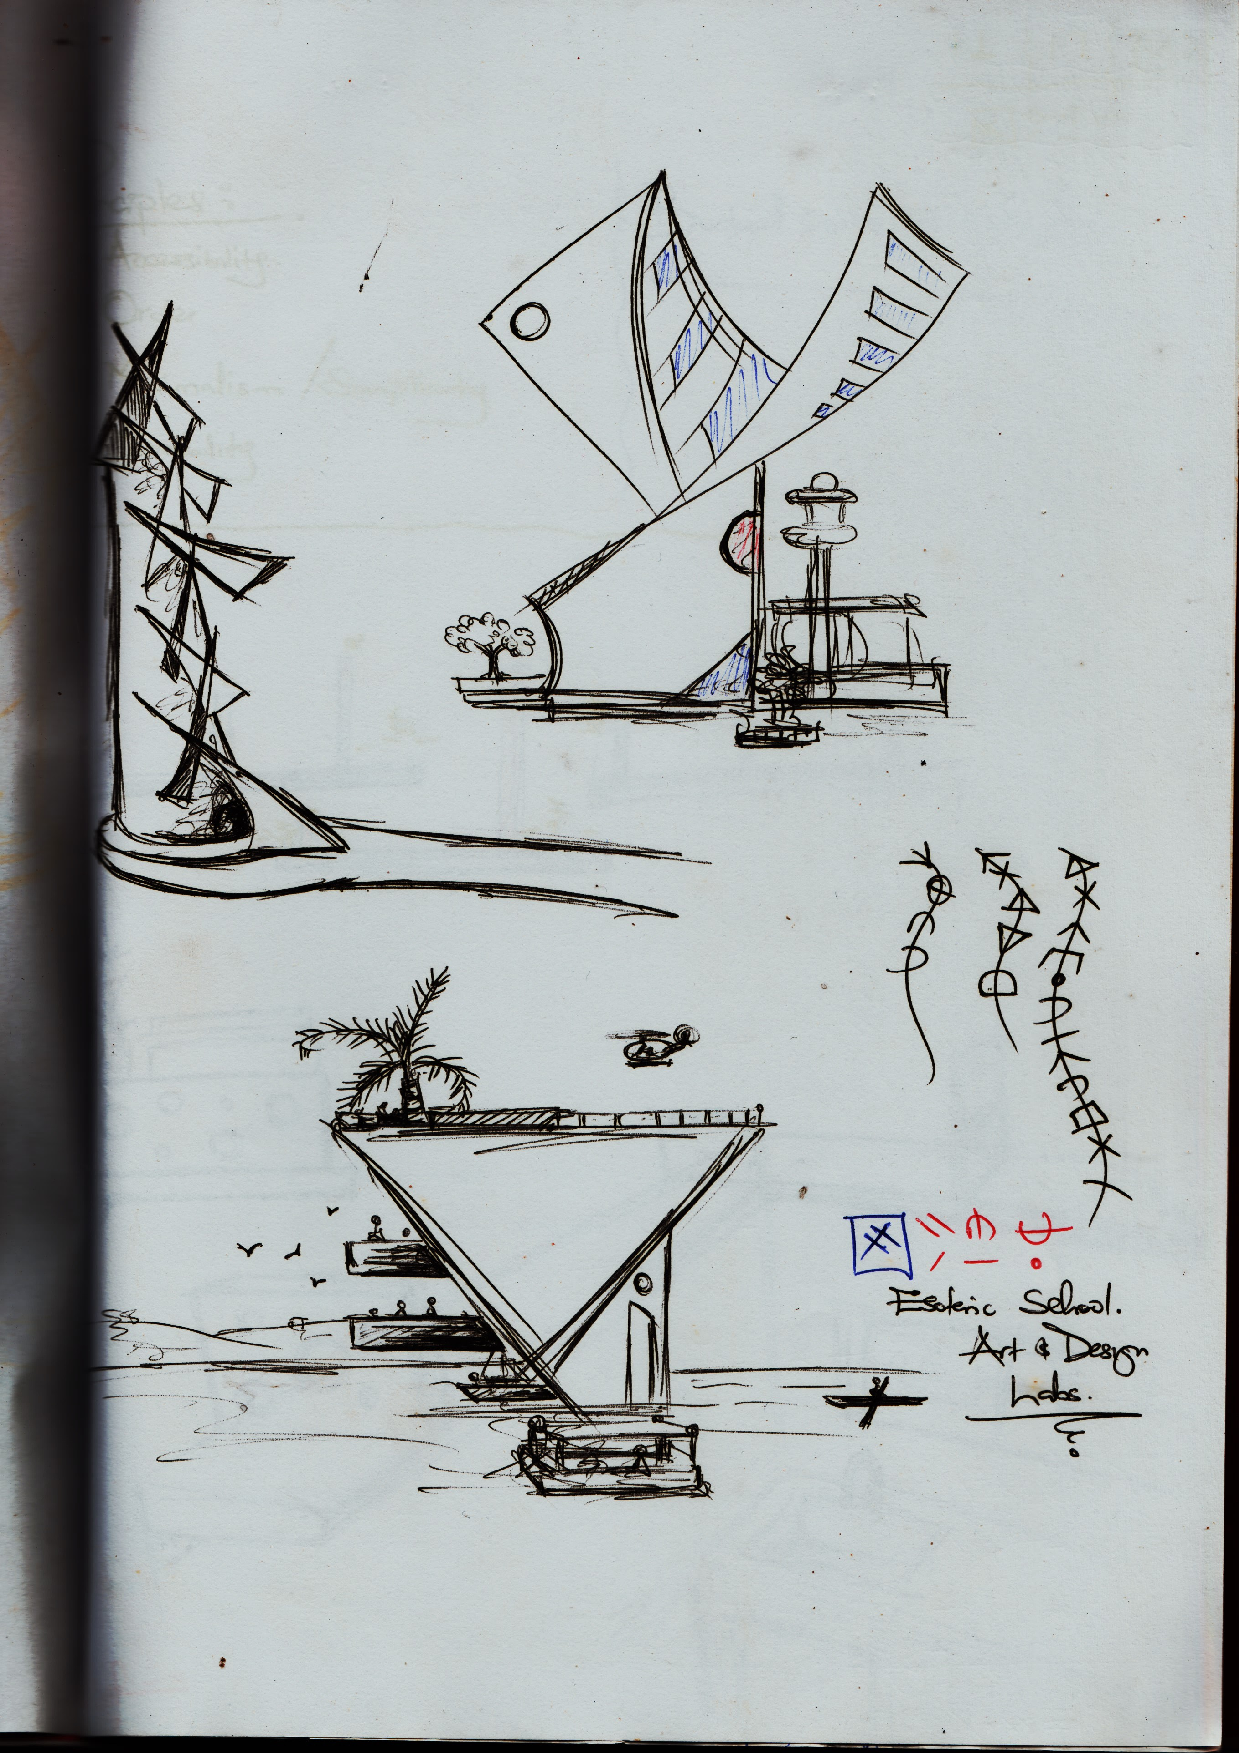
\includegraphics[trim=0cm 4cm 0cm 2.8cm, clip, width=0.9\textwidth,]{resources/pdfs/ozin_gene_expressions.pdf}\\
   \caption{An excerpt from architectural design notes by the author from early days of his home-based research laboratory. In this note, we also get to see an idea similar to how gene expressions are actually a chain of glyphs that, as in our \textbf{LGES} protocols, are depicted as structures chained to each other along a \textit{backbone structure} symbolically depicted as a line (curved lines in this case). Copyrights due to author and Nuchwezi Research Labs.}
  \label{FIGCODEOZINART}
  \end{center}
\end{figure}


For some, the \textbf{Ozin Cipher}\cite{lutalo_2025_ozin} (see \textbf{Section \ref{SECOZIN}}) might not seem that important or useful, but, perhaps because not everyone can immediately appreciate the fact that cryptography is such a dear part of expression in nature, that whoever is the Architect of Life, has applied it throughout nature in many creative ways --- camouflage in reptiles and viruses, the occult languages of birds, etc. And these phenomena have indeed inspired many observant minds throughout the ages, to pick a leaf from nature and apply these ideas (in \textit{alternative information expression}) in everything including mathematics, philosophy and yes... \textit{magick}! Talking of which, for those interested in getting a deeper idea concerning how such a beautiful numeric symbol system --- an alternative to the commonplace Arabic Numerals, came to be, one useful resource is the \textbf{CODE OGF}\cite{lutalo_2025_ogf}.

\begin{figure}[H]
  \begin{center}
  %\includegraphics[trim=2cm 8cm 2cm 8cm, clip, width=0.9\textwidth,]{resources/pdfs/ProteinSynthesisStateMachine.pdf}\\
   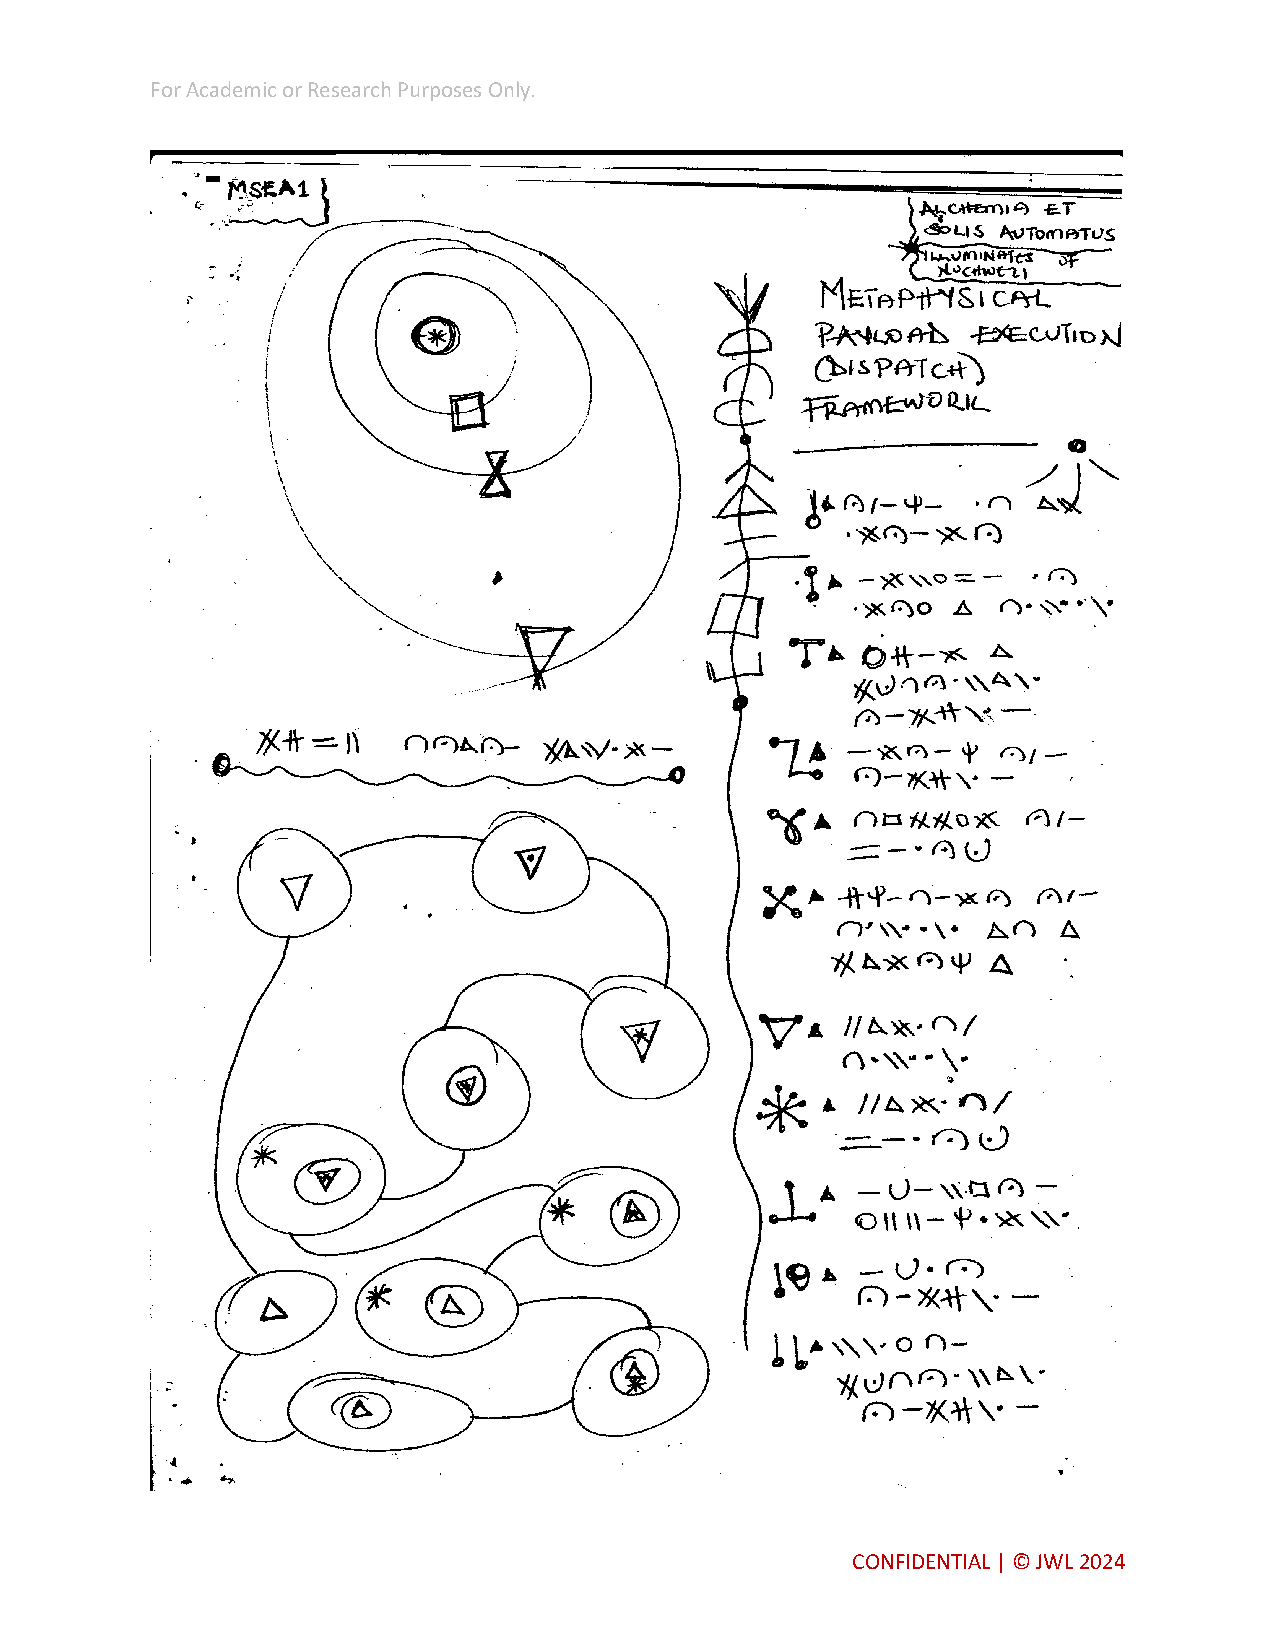
\includegraphics[trim=0cm 2cm 0cm 0cm, clip, width=0.9\textwidth,]{resources/pdfs/ozin.pdf}\\
   \caption{The OZIN Cipher in use. An excerpt from the Church of Dance Eternal OGF}
  \label{FIGCODEOZIN}
  \end{center}
\end{figure}

\textbf{Figure \ref{FIGCODEOZIN}} is just an excerpt from that manuscript, perhaps not so clear because the original manuscript is handwritten\footnote{Some of these notes do have a life of their own though. So, for example, if one wishes to look at a clear scanned version of \textbf{\hyperref[FIGCODEOZINART]{Figure \ref{FIGCODEOZINART}}}, there is a copy at the author's online Art Portfolio --- \url{https://www.deviantart.com/nemesisfixx/art/Not-So-Impossible-Dwellings-823360670}, and as for \textbf{\hyperref[FIGCODEOZINNOTES]{Figure \ref{FIGCODEOZINNOTES}}}, a clear version is also curated at \url{https://www.deviantart.com/nemesisfixx/art/Nu-Druid-Calligraphy-806645934}}, and this is just a scanned version. But hopefully it drives the point home. Also, as seen from that excerpt as well as a closely related excerpt --- see \textbf{Figure \ref{FIGCODEOZINNOTES}}, just like we might replace numbers with alternative symbols, we also see the Latin Alphabet replaced by an ``alien-looking" hand, and this might definitely have its place in transformations of $\psi_{az}$ sequences or their expression in other ways! 


\begin{figure}[H]
  \begin{center}
  %\includegraphics[trim=2cm 8cm 2cm 8cm, clip, width=0.9\textwidth,]{resources/pdfs/ProteinSynthesisStateMachine.pdf}\\
   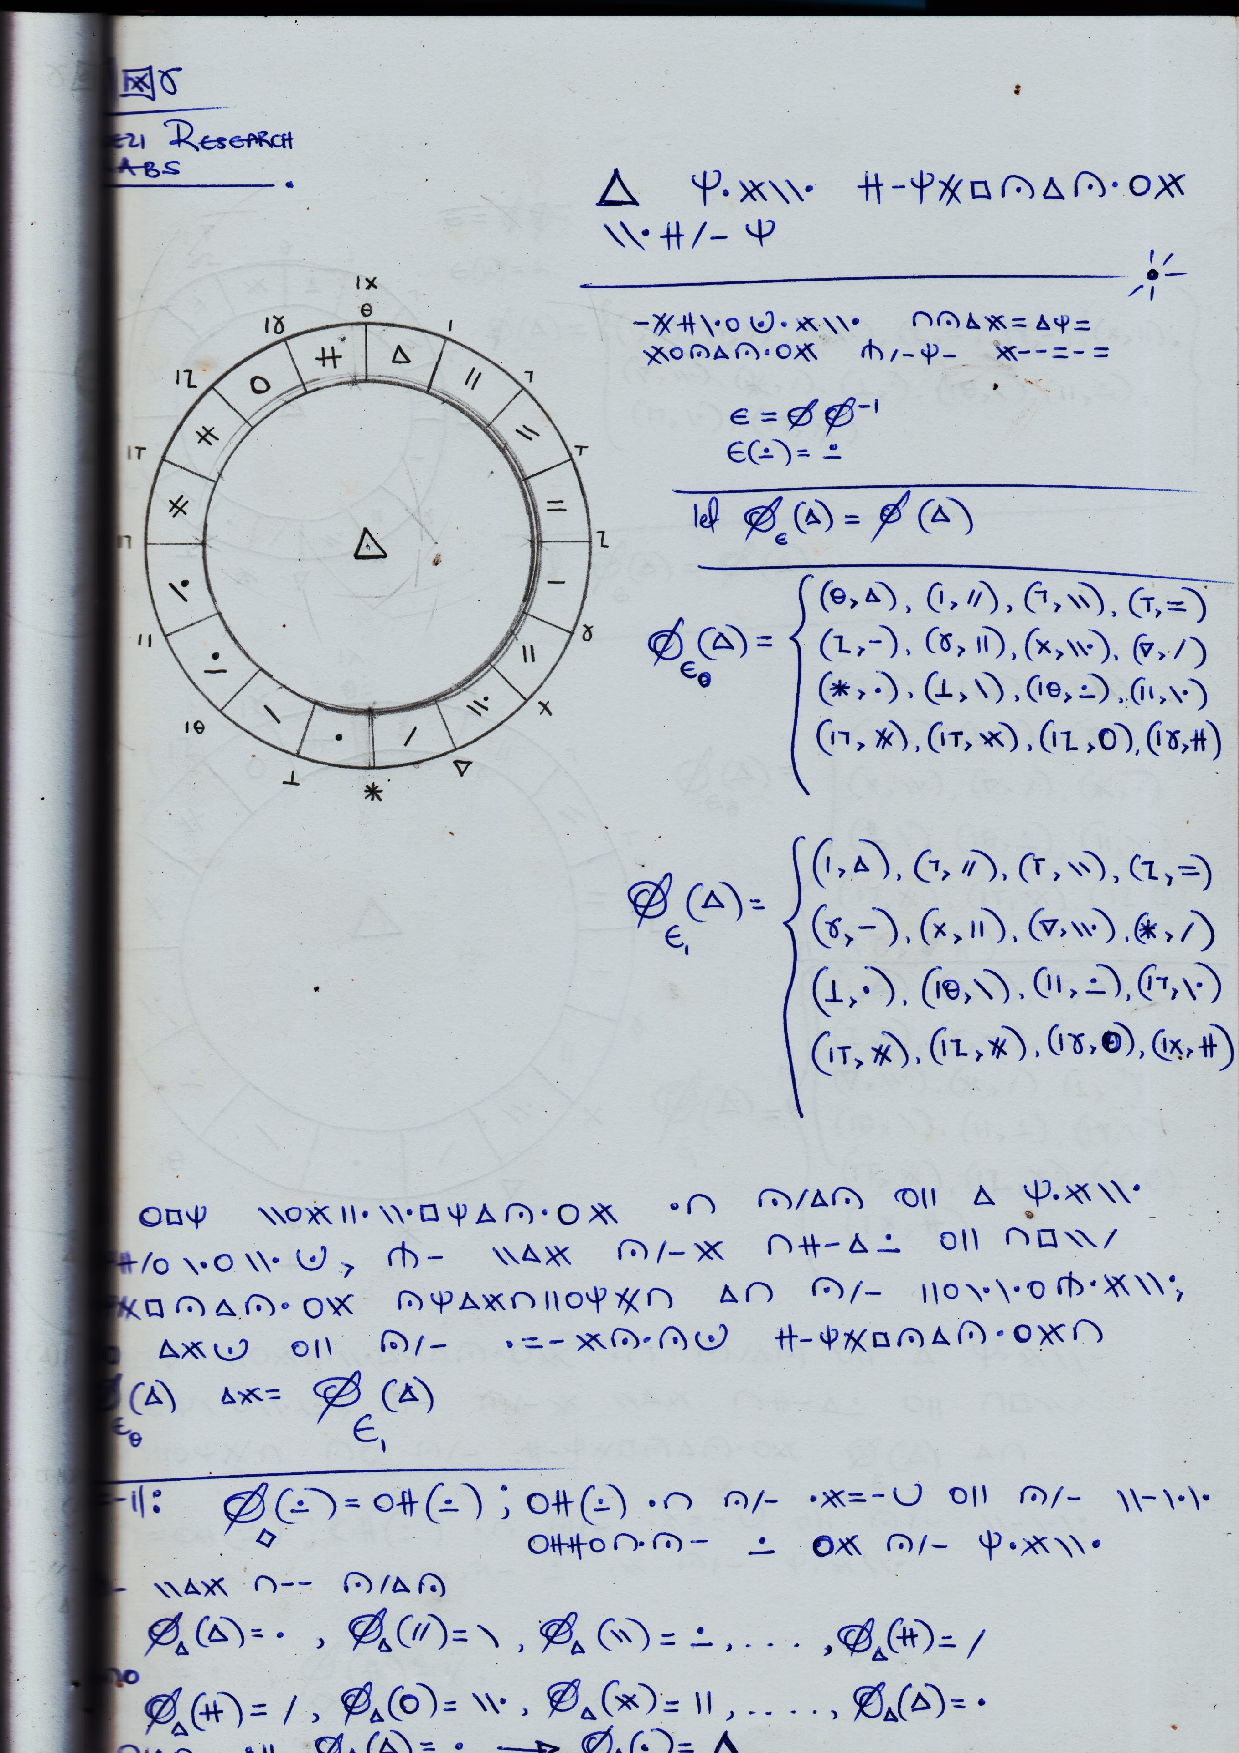
\includegraphics[ width=0.9\textwidth,]{resources/pdfs/ozin_applied.pdf}\\
   \caption{The OZIN Cipher in use. An excerpt from author's research notes (circa 2019) on developing a cryptographic system leveraging a dial mechanism. Copyrights due to author and Nuchwezi Research Labs.}
  \label{FIGCODEOZINNOTES}
  \end{center}
\end{figure}

\chapter{Computing Platonic-Form Encoding Keys (PFEKs), $\boxed{\psi_\Omega}_m$ for a Particular na-Sequence $\Theta$ or $m$}
\label{SECIFAMSSPFMAPS}


It is one of the tricky, but otherwise readily solvable aspects of the \textbf{Lu-Genome Expression System} (LGES), that when constructing the \textbf{BODY} aspect of a \textbf{Full Genome Expression} (FGE) corresponding to a particular sequence $\Theta$, that we correctly pick or generate the corresponding platonic-form encoding key, $\boxed{\psi_\Omega}_m$, that corresponds to the sequence's characteristic, or rather, the \textbf{modal sequence}. 


In particular, we use the concept of shuffling/anagrammatizing a sequence relative to some initial/specific input \textbf{partitioning index} $k$ --- in this case $m$, derived as such:

\begin{equation}
 m = \invpi(\overset{>}{\Theta})
\end{equation}\\

So that, for the case of rendering \textbf{FGE} basing on some sequence $\Theta$ --- possibly an na-Sequence, encoded (for \textbf{LGES}) using base-$\Omega$, we use the \textbf{Second Lu-Shuffle Algorithm} (SLSA) --- introduced in \textbf{\hyperref[APPSLSA]{Section \ref{APPSLSA}}}, and for which important example look-up-tables are shown in \textbf{\hyperref[SECAPPLYSLSA]{Section \ref{SECAPPLYSLSA}}}, to anagrammatize $\psi_\Omega$ \textbf{relative to} $m$, so as to arrive at a correct $\boxed{\psi_\Omega}_m$ that we then use to render the \textbf{FPA} for $\Theta$. Essentially, we must compute the transform:\\


\begin{trans}[Generating the \textbf{Platonic-Form Encoding Key}]
$ $\\
$\psi_\Omega \xrightarrow{slsa(\psi_\Omega, m)} \boxed{\psi_\Omega}_m$\\
\end{trans}
 
Where $slsa(\Theta,m)$ is equivalent to invoking \texttt{lu\_shuffler\_b$(\Theta,m)$} as examples in \textbf{\hyperref[LST_SLSA]{Listing \ref{LST_SLSA}}} show. 

Good enough, we not only have ready-to-use shuffled versions of $\psi_\Omega$ = $\psi_{10}$ = $\langle 0, 1, 2, 3, 4, 5, 6, 7, 8, 9 \rangle$ as shown in \textbf{\hyperref[FIGTRACESLSA]{Figure \ref{FIGTRACESLSA}}}, but also, in case one wishes to manually compute or perhaps automatically generate the necessary key for a given $m$ or \textit{any} sequence, the Python program in \textbf{\hyperref[LST_SLSA]{Listing \ref{LST_SLSA}}} can be utilized for this purpose.
 

That said, basing on the algorithm that generated the mappings in textbf{\hyperref[FIGTRACESLSA]{Figure \ref{FIGTRACESLSA}}}, we have ready-to-use \textbf{Platonic-Form Encoding Keys} corresponding to particular values of $m$ as shown in the following table.\\


\begin{table}[H]
  \centering
  \Large
	\begin{tabular}[t]{|p{6cm}||c|c|c|c|c|c|c|c|c|c|}
	\hline
	\multicolumn{11}{|c|}{\textbf{PFEK Look-up Table by FLSA}}\\
	\hline
	\hline
	\diagbox{$m = \invpi(\overset{>}{\Theta})$}{$I(\omega_i,\overset{>}{\Theta})$} & 1 & 2 & 3 & 4 & 5 & 6 & 7 & 8 & 9 & 10\\
	\hline
	\hline
	1 & \textbf{9} & 7 & 4 & 0 & 5 & 3 & 8 & 2 & 1 & 6\\ 
	\hline 
	2 & \textbf{9} & \textbf{7} & 4 & 0 & 5 & 3 & 8 & 2 & 1 & 6\\ 
	\hline 
	3 & \textbf{8} & \textbf{6} & \textbf{3} & 9 & 4 & 2 & 7 & 1 & 0 & 5\\ 
	\hline 
	4 & \textbf{8} & \textbf{6} & \textbf{3} & \textbf{9} & 4 & 2 & 7 & 0 & 1 & 5\\
	\hline
	5 & \textbf{5} & \textbf{3} & \textbf{0} & \textbf{6} & \textbf{1} & 7 & 4 & 8 & 9 & 2\\
	\hline
	6 & \textbf{5} & \textbf{1} & \textbf{2} & \textbf{6} & \textbf{3} & \textbf{7} & 4 & 8 & 9 & 0\\
	\hline 
	7 & \textbf{0} & \textbf{8} & \textbf{9} & \textbf{1} & \textbf{5} & \textbf{2} & \textbf{6} & 3 & 4 & 7\\
	\hline 
	8 & \textbf{3} & \textbf{8} & \textbf{9} & \textbf{4} & \textbf{2} & \textbf{5} & \textbf{6} & \textbf{0} & 1 & 7\\
	\hline
	9 & \textbf{9} & \textbf{1} & \textbf{2} & \textbf{3} & \textbf{8} & \textbf{4} & \textbf{5} & \textbf{6} & \textbf{7} & 0\\ 
	\hline
	10 & \textbf{9} & \textbf{5} & \textbf{6} & \textbf{7} & \textbf{8} & \textbf{0} & \textbf{1} & \textbf{2} & \textbf{3} & \textbf{4}\\
	\hline
	              
\end{tabular}
 \caption{Platonic Form Encoding Keys (PFEK) mapped to corresponding values of $m = \invpi(\overset{>}{\Theta})$ using \textbf{FLSA}}
  \label{TABFSLAPERK}
\end{table}


And if one wishes to render their \textbf{PFA} --- the platonic form aspect, of the \textbf{FGE} using the \textbf{SLSA}, then the corresponding table is as follows:\\


 
\begin{table}[H]
  \centering
  \Large
	\begin{tabular}[t]{|p{6cm}||c|c|c|c|c|c|c|c|c|c|}
	\hline
	\multicolumn{11}{|c|}{\textbf{PFEK Look-up Table by SLSA}}\\
	\hline
	\hline
	\diagbox{$m = \invpi(\overset{>}{\Theta})$}{$I(\omega_i,\overset{>}{\Theta})$} & 1 & 2 & 3 & 4 & 5 & 6 & 7 & 8 & 9 & 10\\
	\hline
	\hline
	1 & \textbf{4} & 2 & 8 & 9 & 0 & 7 & 3 & 6 & 5 & 1\\ 
	\hline
	2 & \textbf{4} & \textbf{2} & 8 & 9 & 0 & 7 & 3 & 6 & 5 & 1\\ 
	\hline
	3 & \textbf{7} & \textbf{5} & \textbf{3} & 0 & 8 & 2 & 6 & 1 & 9 & 4\\ 
	\hline
	4 & \textbf{1} & \textbf{6} & \textbf{4} & \textbf{7} & 2 & 9 & 0 & 3 & 8 & 5\\ 
	\hline
	5 & \textbf{2} & \textbf{1} & \textbf{0} & \textbf{6} & \textbf{8} & 3 & 5 & 4 & 7 & 9\\ 
	\hline
	6 & \textbf{7} & \textbf{1} & \textbf{2} & \textbf{4} & \textbf{6} & \textbf{8} & 3 & 9 & 0 & 5\\ 
	\hline
	7 & \textbf{5} & \textbf{9} & \textbf{2} & \textbf{3} & \textbf{7} & \textbf{0} & \textbf{4} & 6 & 1 & 8\\ 
	\hline
	8 & \textbf{9} & \textbf{1} & \textbf{5} & \textbf{4} & \textbf{3} & \textbf{2} & \textbf{7} & \textbf{8} & 6 & 0\\ 
	\hline
	9 & \textbf{5} & \textbf{6} & \textbf{3} & \textbf{9} & \textbf{0} & \textbf{4} & \textbf{2} & \textbf{7} & \textbf{1} & 8\\ 
	\hline
	10 & \textbf{6} & \textbf{3} & \textbf{8} & \textbf{2} & \textbf{1} & \textbf{9} & \textbf{7} & \textbf{4} & \textbf{0} & \textbf{5}\\
	              \hline
\end{tabular}
 \caption{Platonic Form Encoding Keys (PFEK) mapped to corresponding values of $m = \invpi(\overset{>}{\Theta})$ using \textbf{SLSA}}
  \label{TABSSLAPERK}
\end{table}

\subsection{Example of Resolving PFA Components, $\boxed{\omega_i^*}$}

We shall not attempt to render a complete \textbf{FGE} here since that matter is already well catered for in the associated chapter and section --- see \textbf{\hyperref[SECFULLGES]{Section \ref{SECFULLGES}}}, however, we shall attempt to set straight, the necessary procedure for:

\begin{enumerate}
\item{Computing $m$ for a given $\Omega$-encoded sequence $\Theta$:

\begin{enumerate}
\item Compute the \textbf{modal sequence statistic}, $\overset{>}{\Theta}$ --- see \textbf{Definition 1} in \cite{transformatics}.
\item Compute $m$ from the cardinality of the modal sequence as: $m = \invpi(\overset{>}{\Theta})$.
\end{enumerate}
}
\item {Picking the correct \textbf{PFEK} for that $m$ --- i.e. $\boxed{\psi_{pf}}_m$:
	\begin{enumerate}
	\item If using \textbf{FLSA}, refer to \textbf{\hyperref[TABFSLAPERK]{Table \ref{TABFSLAPERK}}}, and for any $m = k$, pick the row for which the first column has the value $k$.
	\item Of course, for any $m = k$, the only useful values on that row for doing the \textbf{PFEK} operations are the \textbf{first $k$ emboldened} values on the row corresponding to $m$. E.g. for $m=2$ the necessary key is just $\langle 9, 7 \rangle$, not the entire row.
	\item If using \textbf{SLSA}, lookup the \textbf{PFEK} using \textbf{\hyperref[TABSSLAPERK]{Table \ref{TABSSLAPERK}}}, so that, for $m = 2$, we have $\boxed{\psi_{pf}}_2 = \langle 4, 2 \rangle $
	\end{enumerate}
}
\item{ Resolving the correct component from $\boxed{\psi_{pf}}_m$ corresponding to a particular element $\omega_i$ in the corresponding \textbf{IFA MSS}, $\overset{>}{\Theta}$.
\begin{enumerate}
\item So, if our \textbf{IFA MSS} was just $\langle 0, 2, 1, 3, 6 \rangle$ such as for $\Omega_{3}$ from \textbf{Equation \ref{EQDNEXA}}, then taking note of the special case for any $\omega_i^* = 0$ --- such as the first term in this case (see \textbf{Step\#2(e)ii} in \textbf{\hyperref[ALGCOZINPLATO]{Algorithm \ref{ALGCOZINPLATO}}}), we merely map values of `0' in the \textbf{MSS} to just the \textbf{JOINT/GAP} element in \textbf{Figure \ref{FIGPLATONICCIPH}}), for the other terms, such as $\omega_3^* = 3$, since the corresponding \textbf{PFEK} for $m=5$ is $\boxed{\psi_{pf}}_5 = \langle 2, 1, 0, 6, 8 \rangle $, then $\boxed{\omega_3^*} = 0$ as per the corresponding look-up mapping we see for such an \textbf{MSS}:


\[
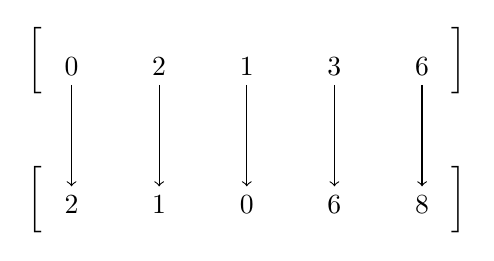
\begin{tikzpicture}[baseline=(current bounding box.center)]
  % Matrix A
  \matrix (A) [matrix of math nodes, left delimiter={[}, right delimiter={]}, row sep=1em, column sep=2em] {
    0 & 2 & 1 & 3 & 6 \\
  };

  % Matrix B
  \matrix (B) [matrix of math nodes, left delimiter={[}, right delimiter={]}, row sep=1em, column sep=2em, below=3em of A] {
    2 & 1 & 0 & 6 & 8\\
  };

  % Draw arrows from A_i to B_i
  \foreach \i in {1,2,3,4,5}
    \draw[->] (A-1-\i) -- (B-1-\i);
\end{tikzpicture}
\]

And so, for the last term in that \textbf{MSS}, $\boxed{\omega_5^*} = 8$

\end{enumerate}
}

\item{How to render the final pf-encoded version of $\omega_i^*$, i.e. $\boxed{\omega_i^*}$.
\begin{enumerate}
\item So, now that you know the \textbf{PFEK} for your $m$, such as $\boxed{\psi_{pf}}_5 = \langle 2, 1, 0, 6, 8 \rangle $ from above, and have the correct pf-term for a particular term in the \textbf{MSS} such as $\boxed{\omega_5^*} = 8$ in the example above, the corresponding pf-term is the platonic structure from \textbf{\hyperref[FIGPLATONICCIPH]{Figure \ref{FIGPLATONICCIPH}}} that corresponds to the index $8$ --- so that would be the \textbf{octagon} or rather \textbf{octa-gram} with nothing at the center. But also, given the term we are decoding is $\omega_5^*$ = 6, then the overall structure would be as per configuration \textbf{$8_{pf} + 8 \times 6_{oz}$}: That is to say:

\begin{equation}
\boxed{\omega_5^*}_{pf} = 8_{pf} \otimes 6_{oz} = 8_{pf} + 8 \times 6_{oz}
\end{equation}

So that the final rendered term for this element alone would be as shown:


\begin{figure}[H]
  \begin{center}
   %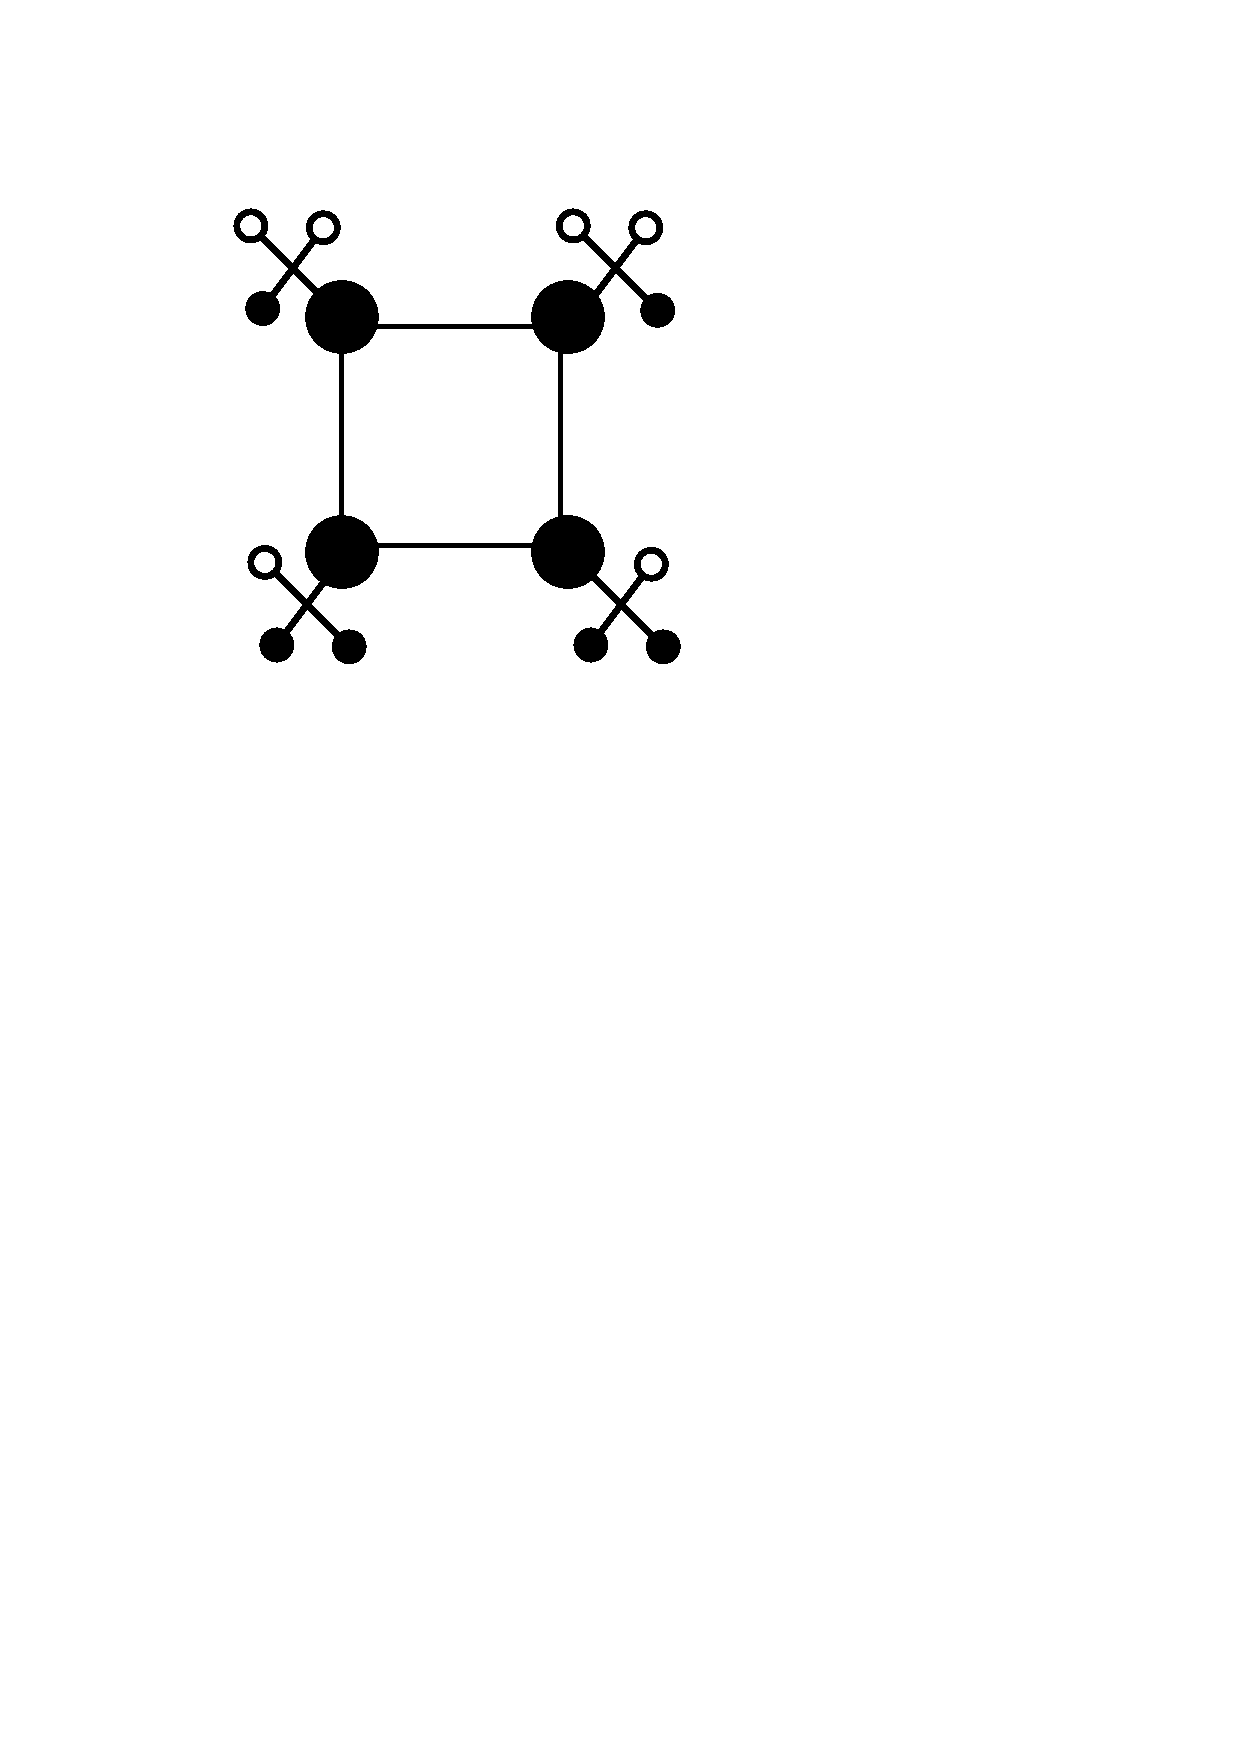
\includegraphics[trim=LEFT BOTTOM RIGHT TOP, clip, width=0.9\textwidth,]{resources/pdfs/EXAPLATONICFORM-PFA.pdf}\\
   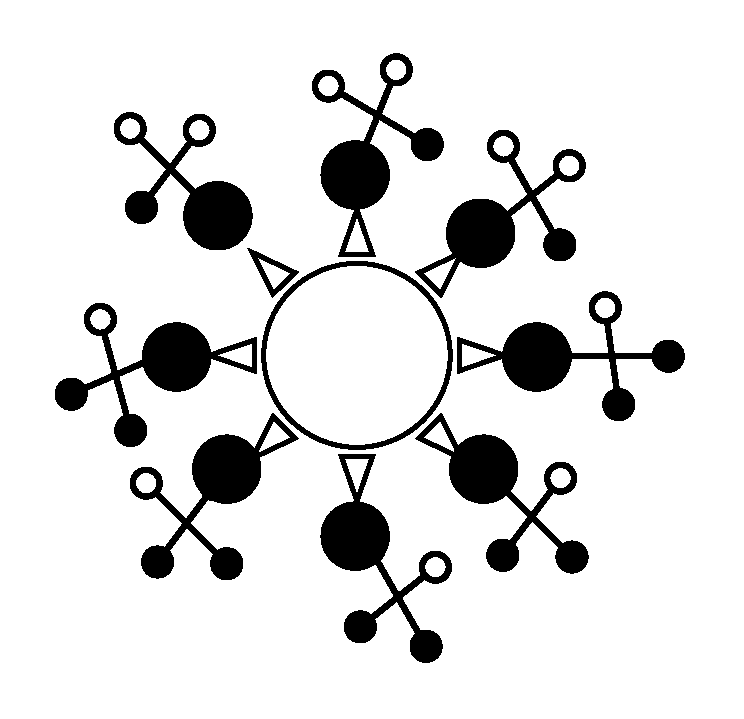
\includegraphics[ width=0.9\textwidth,]{resources/pdfs/EXAPLATONICFORMPFA_OCT.pdf}\\
   \caption{An example of a single \textbf{PFA} component equivalent to the configuration \textbf{$8_{pf} \otimes 6_{oz}$}.}
  \label{FIGEXAPLATONICFORMPFA_OCT}
  \end{center}
\end{figure}



\end{enumerate}
}
\end{enumerate}

Of course, once one has the correct $\boxed{\omega_i^*}$, they can just attach it to the existing \textbf{FGE} chain-structure so as to construct the  complete \textbf{BODY} aspect of a full genome expression for $\Theta$.




\chapter{Alternative[ORIGINAL] $\Omega$-to-PLATONIC Form Genetic Code Expression Algorithm}
\label{SECALTPFGESA}

While developing the theory for the \textbf{Lu-Genome Expression System}, and particularly while and after looking at the way the original concept of the algorithm for generating the BODY-components of the \textbf{FGE} was working --- for example, it uses the \textbf{IFA MSS} as key to pick corresponding platonic form structures from $\lnot(\psi_{pf})$ and not directly from $\psi_{pf}$, because the idea is that, the most frequent term in the \textbf{IFA MSS} should correspond to a \textit{larger} or \textit{more prominent} or \textit{more complex} geometric form than the least significant terms. And thus, we shall see that, since natural genetic sequences (or rather, DNA-sequences) only span $\psi_{DNA}$ which has only 4 distinct symbols, then we would never have a meaningful way to utilize the complete set of 10 distinct geometrical structures from $\psi_{pf}$ --- one interesting consequence of \textbf{\hyperref[ALGCOZINPLATO_ORIG]{Algorithm \ref{ALGCOZINPLATO_ORIG}}} (particularly \textbf{\hyperref[EQFBOXED_ORIG]{Equation \ref{EQFBOXED_ORIG}}}) that performs the translation from \textbf{mRNA}-equivalent $\Omega$-encoded \textbf{IFA MSS} to geometric $pf$-encoded \textbf{PFA}, using the $\lnot(\psi_{pf})$, is that (\textbf{irrespective} of the organism or species we would look at) it seems as though the resulting \textbf{PFA} expressions \textbf{must} always \textbf{only} utilize the \textbf{first four} elements of $\lnot(\psi_{pf})$ --- $\langle 9, 8, 7, 6 \rangle$, since all possible \textbf{IFA MSS} would only have utmost $4$ distinct symbols in them. And if we had not used $\lnot(\psi_{pf})$, still, a direct use of $\psi_{pf}$ would only utilize the start of that symbol set if we map elements in $\psi_\Omega$ to those in $\psi_{pf}$, thus why we returned to the drawing board, and developed \textbf{\hyperref[ALGCOZINPLATO]{Algorithm \ref{ALGCOZINPLATO}}} instead.

Studying the resulting genome expressions visually, one would find that it seems like we always express the BODY of any \textbf{FGE} with some structure containing a \textbf{nucleus}\footnote{Of course, the way the platonic forms corresponding to \textbf{9} and \textbf{7} were simplified to those of \textbf{8} (octagon-\textit{chaosstar}-octagram) and \textbf{6}(hexagon-\textit{hexagram}) respectively, with \textbf{the twist} that the \textbf{extra appendage point is placed at the center of the geometric structure instead of creating an extra vertex/appendage point}. It does have some good justification though --- \textit{\textbf{Occam's Razor} principle in a way, but also that, while observing nature, we typically find that \textbf{Simple is Better}}. Nonetheless, the sensibilities of mapping any $i$ in $\psi_{10}$ or rather $\psi_\Omega$ to a platonic form corresponding to \textbf{the regular polygon with internal angle} corresponding to $\frac{360}{i}$ still makes sense for all 10 terms in $\psi_\Omega$.}\footnote{The inverse would be \textbf{BODY} made of mostly gaps and/or joints, basic linear structures and triangles!}!

We shall keep that original algorithm here, for mostly study/comparison purposes...

\begin{alg}[The \textbf{$\Omega$-to-PLATONIC Form Genetic Code Expression Algorithm}]
\label{ALGCOZINPLATO_ORIG}

Assuming we have an $\Omega$-base encoded genetic code sequence $\Theta_\Omega$ of some length $n > 0$.

\begin{enumerate}
\item{Initialize the expression with a transcription, by Using \textbf{Algorithm \ref{ALGCOZIN}} to construct the \textbf{Intermediate Form Affix} (IFA) of $\Theta_\Omega$ --- essentially return $OZ(\Theta_\Omega)$ as the start of the \textbf{Final Genome Expression} (FGE) $\boxed{OZ(\Theta_\Omega)}^*$ --- so that the final complete expressed(transcribed+translated ) sequence shall be as:\\

\begin{equation}
\label{EQTRANSLGENSEQ_ORIG}
\boxed{OZ(\Theta_\Omega)}^* = OZ(\Theta_\Omega)\cdot\boxed{OZ(\Theta_\Omega)}
\end{equation}\\

$\boxed{OZ(\Theta_\Omega)}: \mathbb{N} \times \psi_{pf}$ is the suffix of expressed na-Sequence $\Theta_\Omega$, and is expressed in our genome expression system, as PLATONIC-Form encoded \textbf{modal sequence statistic} of $OZ(\Theta_\Omega)$\footnote{We render the \textbf{suffix of FGE} as $\overset{>}{OZ(\Theta_\Omega)}$ because it allows us to not express $\Theta_\Omega$ naively at the genome or gene level, but also, so that, from an information-theoretic perspective, the completed genome expression is somewhat a statistical summary of what the genome sequence contains --- the appearance of an animal or a plant or virus, depicting or expressing the summary of its DNA code. We do this then, by not merely doing a 1-to-1 translation of the intermediate Ozin-code expression $OZ(\Theta_\Omega)$, but instead computing its summary in form of $\overset{>}{OZ(\Theta_\Omega)}$, and then instead translating that into the final spatial/geometric forms as per $\psi_{pf}$. This shall then help complete the entire processing/synthesis of sequence $\Theta_\Omega$, or rather our genome expression.} --- the \textbf{PFA}\footnote{Platonic Form Aspect}, i.e.:\\

\begin{equation}
 \boxed{OZ(\Theta_\Omega)} = \boxed{\overset{>}{OZ(\Theta_\Omega)}}_{pf}
\end{equation}\\


}
\item{ So once we have the \textbf{IFA}, $OZ(\Theta_\Omega)$, proceed to use it to generate the rest of the sequence expression as follows: 
\begin{enumerate}
\item {\textbf{INITIALIZE} FGE, $\boxed{OZ(\Theta_\Omega)}^*$ as just:\\

\begin{equation}
\label{EQSTARTFGE_ORIG}
\boxed{OZ(\Theta_\Omega)}^* = \langle \langle OZ(\Theta_\Omega) \rangle \langle \rangle \rangle
\end{equation}\\

This ensures, we have the prefix affix, \textbf{IFA}, as the contents of the sequence start of \textbf{FGE} \textit{extended} by a \textbf{still empty subsequence} --- in expression form, this shall merely be a backbone structure with \textbf{IFA} as its head, and a terminal that is ready to have more units appended to it, \textbf{after a single GAP/JOINT extension to IFA}. So, it also means, at this juncture, \textbf{PFA} is just:\\

\begin{equation}
\label{EQSTARTFGESUF_ORIG}
\boxed{OZ(\Theta_\Omega)} = \langle \rangle
\end{equation}\\

}
\item {
	\textbf{COMPUTE} the \textbf{IFA MSS}, $\overset{>}{OZ(\Theta_\Omega)}$
}
\item{\textbf{FOREACH} symbol/term $\omega_i^*$ in \textbf{IFA MSS}, $\overset{>}{OZ(\Theta_\Omega)}$: 
\begin{enumerate}
\item{\textbf{USE} the translation mapping: $\psi_\Omega \rightarrow \lnot(\psi_{pf}) \rightarrow \psi_{pf}$ as depicted in \textbf{Figure \ref{FIGPLATONICCIPH}}, to translate $\omega_i^*$ into the equivalent \textbf{Platonic Form}, $\boxed{\omega_i^*}$ for the final code as such:}
\item { \textbf{IF} $\omega_i^* \equiv 0$:Operating on the current \textbf{FGE}: 
		\begin{enumerate}
		\item { Append/Insert a JOINT onto \textbf{FGE},  $\boxed{OZ(\Theta_\Omega)}^*$

		\begin{equation}
		\label{EQEXTFGEJOINT_ORIG}
		\boxed{OZ(\Theta_\Omega)}^* = \boxed{OZ(\Theta_\Omega)}^* \cdot \boxed{\omega_i^*}_{joint}
		\end{equation}		
		
		And equivalently:
		
		\begin{equation}
		\label{EQEXTFGEJOINTSUF_ORIG}
		\boxed{OZ(\Theta_\Omega)} = \boxed{OZ(\Theta_\Omega)} \cdot \boxed{\omega_i^*}_{joint}
		\end{equation}				
		
		}
		\item \textbf{PROCEED} to the next symbol in \textbf{IFA MSS}, $\overset{>}{OZ(\Theta_\Omega)}$\\ (loop from \textbf{Step\#2(c))}.
		\end{enumerate}
	}
	\item { \textbf{ELSE}: \textbf{resolve} the correct  $\boxed{\omega_i^*}$  for  $\omega_i^*$  by using the relation:\\

\begin{equation}
\label{EQFBOXED_ORIG}
 \boxed{\omega_i^*} = \rho_j +  j \times \omega_i^* : j = I(\rho_j,\lnot(\psi_{pl})) = I(\omega_i^*,\psi_\Omega)
\end{equation}\\

	\begin{enumerate}
	\item{\textbf{PLACE} that encoded version, $\boxed{\omega_i^*}$, along the existing \textbf{FGE} structure at the next vacant position ($\invpi(\Theta_\Omega)+i$). Expressible with another version of \textbf{Equation \ref{EQEXTFGEJOINT}} as:
	
	\begin{equation}
	\label{EQEXTFGEPF_ORIG}
		\boxed{OZ(\Theta_\Omega)}^* = \boxed{OZ(\Theta_\Omega)}^* \cdot \boxed{\omega_i^*}
		\end{equation}	
		
		And equivalently:
		
		\begin{equation}
		\label{EQEXTFGEPFSUF_ORIG}
		\boxed{OZ(\Theta_\Omega)} = \boxed{OZ(\Theta_\Omega)} \cdot \boxed{\omega_i^*}
		\end{equation}	
		
	Where the special term, $\boxed{\omega_i^*}$, as per \textbf{Equation \ref{EQFBOXED}}, is basically the PLATONIC Form corresponding to position $j$ in $\lnot(\psi_{pf})$ --- a \textbf{complement/inverted symbol set}, thus one of the final form platonic geometry structures, but also with the intermediate form $\omega_i^*$ expressed $j$ times as an attachment to $\rho_j$, such that:\\
	
	\begin{equation}
	0 \leq (j = (\invpi(\psi_{pf})-i)) \leq (\invpi(\psi_{pf}) = \invpi(\psi_\Omega)) \geq \invpi(\overset{>}{OZ(\Theta_\Omega)})
	\end{equation}\\
	
	
	as depicted in example \textbf{Figure \ref{FIGEXAPLATONICFORMPFA}}, with each expression of $\omega_i^*$ attached to one of the $j$ \textbf{appendage spots} on the shape for $\boxed{\omega_i^*}$.
	}
	\item \textbf{PROCEED} to the next symbol in \textbf{IFA MSS}, $\overset{>}{OZ(\Theta_\Omega)}$\\ (loop from \textbf{Step\#2(c))}.
	\end{enumerate}
	}
\end{enumerate}
}
\end{enumerate}
}

\item \textbf{TRUNCATE} the final-structure after the final term in \textbf{FGE}.
\item \textbf{RETURN} \textbf{FGE}, $\boxed{OZ(\Theta_\Omega)}^*$ as the final transcribed and translated version of $\Theta_\Omega$. The culmination of our conceptual genome expression.
\end{enumerate}
$\qed$
\end{alg}


\begin{center}
\fbox{\begin{minipage}{0.9\textwidth}
\large
\textbf{NOTE:}\\
 
Besides the introductory notes about this alternative algorithm given at the start of this chapter, it might be worth the effort, looking at what kinds of expressions the algorithm can produce so one has a basic means to weigh it against the version we prefer/chose (\textbf{\hyperref[ALGCOZINPLATO]{Algorithm \ref{ALGCOZINPLATO}}} in \textbf{\hyperref[SECGENSEQEXPRES]{Section \ref{SECGENSEQEXPRES}}}). Thus, without delving much into how they were generated, we shall [re-]iterate some of the highlights of how \textbf{\hyperref[ALGCOZINPLATO_ORIG]{Algorithm \ref{ALGCOZINPLATO_ORIG}}} would render various sequences under the \textbf{Lu-Genome Expression System}.

\end{minipage}}
\\
\end{center}



\textbf{IMPORTANT NOTE:} Realize that \textbf{Step\#2(c)iii(A)} of \textbf{Algorithm \ref{ALGCOZINPLATO_ORIG}} processes/operates on the \textbf{IFA MSS}, $\overset{>}{OZ(\Theta_\Omega)}$, and not the \textbf{IFA} directly. This, so that, first of all, we don't process multiple times each term or symbol from the \textbf{IFA} --- which is a direct translation of the genetic code, in the \textbf{PFA}. And then also, the way the translation works, is that if $\omega_x^* > \omega_y^*$ or rather that $|\omega_x^*| > |\omega_y^*|$,  then $\omega_x^*$ shall correspond to a term in $\lnot(\psi_{pf})$ that is simpler\footnote{The idea was somewhat to assign more complex forms to terms in the associated symbol set that occur earlier than others since it somewhat depicts their relative higher significance --- a concept similar to how we would attempt to regenerate a sequence from its modal sequence statistic without say consulting its sequence characteristic --- an inversion of and adaptation of the \textbf{string chart} concept first presented in the \textbf{LOMT-1 Transformer} (\textbf{Transformer 6} in \cite{transformatics}).} in form than $\omega_y^*$ --- higher significance being assigned to earlier-occurrence in the underlying symbol set $\psi_\Omega$. 


Good enough, we have already treated of sequence complements and inverted look-ups in \textbf{Section \ref{SECSIGCOMPLE}}, for this case, the corresponding mapping from terms (or rather, magnitudes) in $\overset{>}{OZ(\Theta_\Omega)}$ to indices in  $\lnot(\psi_{pf})$ is as below --- also stressing the fact that $0 \leq |\omega_i^*| = |\omega_i| < \invpi(\psi_{pf})$ for all $\omega_i \in \Theta_\Omega \quad \land \quad \omega_i^* \in \overset{>}{\Theta_\Omega}$.


\[
\begin{tikzpicture}[baseline=(current bounding box.center)]
  % Matrix A
  \matrix (A) [matrix of math nodes, left delimiter={[}, right delimiter={]}, row sep=1em, column sep=2em] {
    0 & 1 & 2 & 3 & 4 & 5 & 6 & 7 & 8 & 9\\
  };

  % Matrix B
  \matrix (B) [matrix of math nodes, left delimiter={[}, right delimiter={]}, row sep=1em, column sep=2em, below=3em of A] {
    9 & 8 & 7 & 6 & 5 & 4 & 3 & 2 & 1 & 0\\
  };

  % Draw arrows from A_i to B_i
  \foreach \i in {1,2,3,4,5,6,7,8,9,10}
    \draw[->] (A-1-\i) -- (B-1-\i);
\end{tikzpicture}
\]

Looking at some example genome expressions rendered using \textbf{\hyperref[ALGCOZINPLATO_ORIG]{Algorithm \ref{ALGCOZINPLATO_ORIG}}} shall help most reviewers to appreciate whether or not it is better or worse than \textbf{\hyperref[ALGCOZINPLATO]{Algorithm \ref{ALGCOZINPLATO}}}, and whether or not it is better at representing how natural genome expression occurs as seen in our inspiration case --- see \textbf{\hyperref[FIGPINEAPPLE]{Figure \ref{FIGPINEAPPLE}}}.

\subsection{Examples of Complete Lu-Genome Expressions}
\label{SECFULLGES_ORIG}

We get to see the first example of the output of processing some na-Sequence expressed originally in base-$\Omega$ such as for $\Omega_{3}$ from \textbf{Equation \ref{EQDNEXA}}, in its final expression form as in \textbf{Figure \ref{FIGPLATONICEXA_ORIG}}\cite{lutalo_2025_exa} --- more importantly, since we have already seen its \textbf{IFA} (the \textbf{FGE} prefix) in \textbf{Figure \ref{FIGOZEXA}}, we note that we essentially see the update as the result of expressing the entire \textbf{FGE} via the \textbf{IFA MSS} equivalent to:

\begin{equation}
\overset{>}{\Omega_{3}} = \langle 0, 2, 1, 3, 6 \rangle \implies \boxed{OZ(\Omega_{3})} \approx \langle GAP, 7, 8, 6, 3 \rangle
\end{equation}


\begin{figure}[H]
  \begin{center}
  %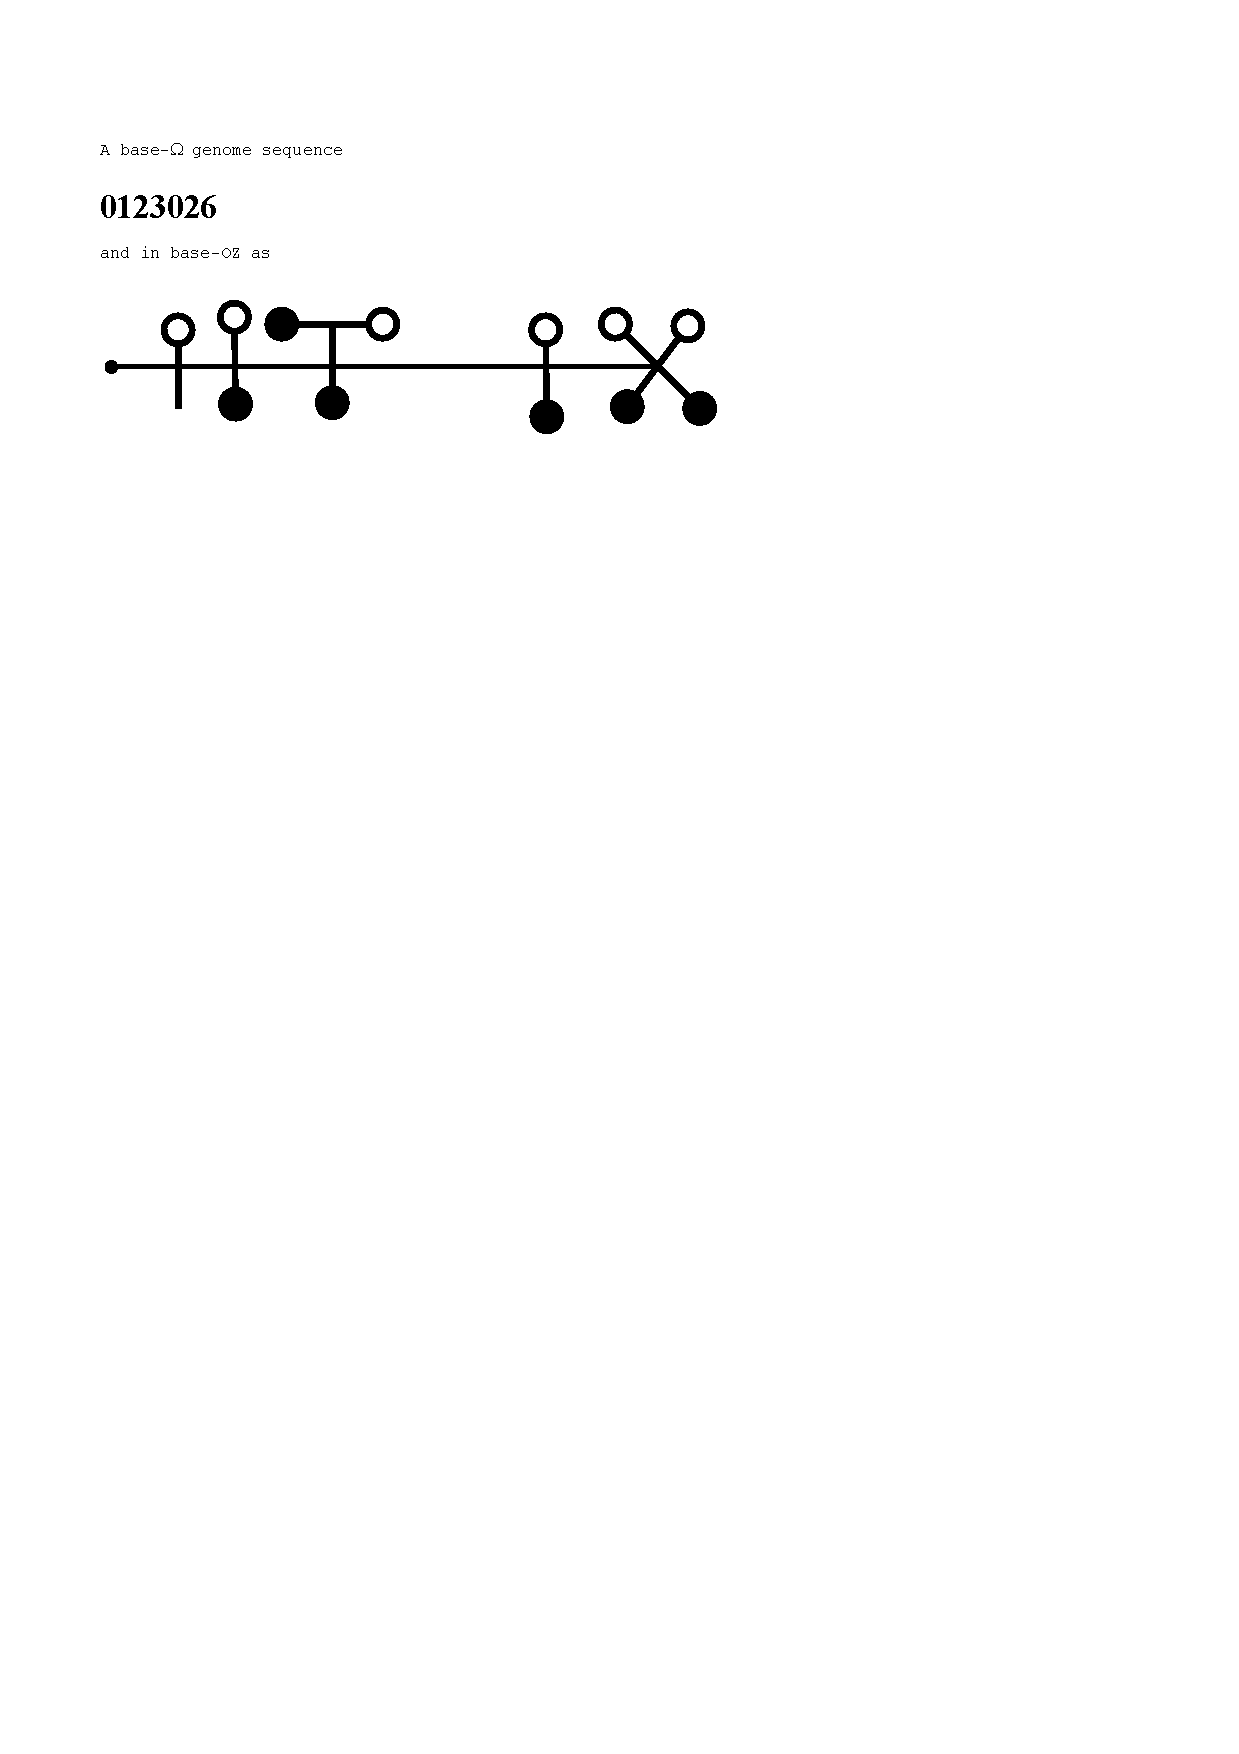
\includegraphics[trim=0cm 20cm 0cm 0cm, clip, width=0.9\textwidth,]{resources/pdfs/OZINCIPHER-APP3-EXA.pdf}\\
   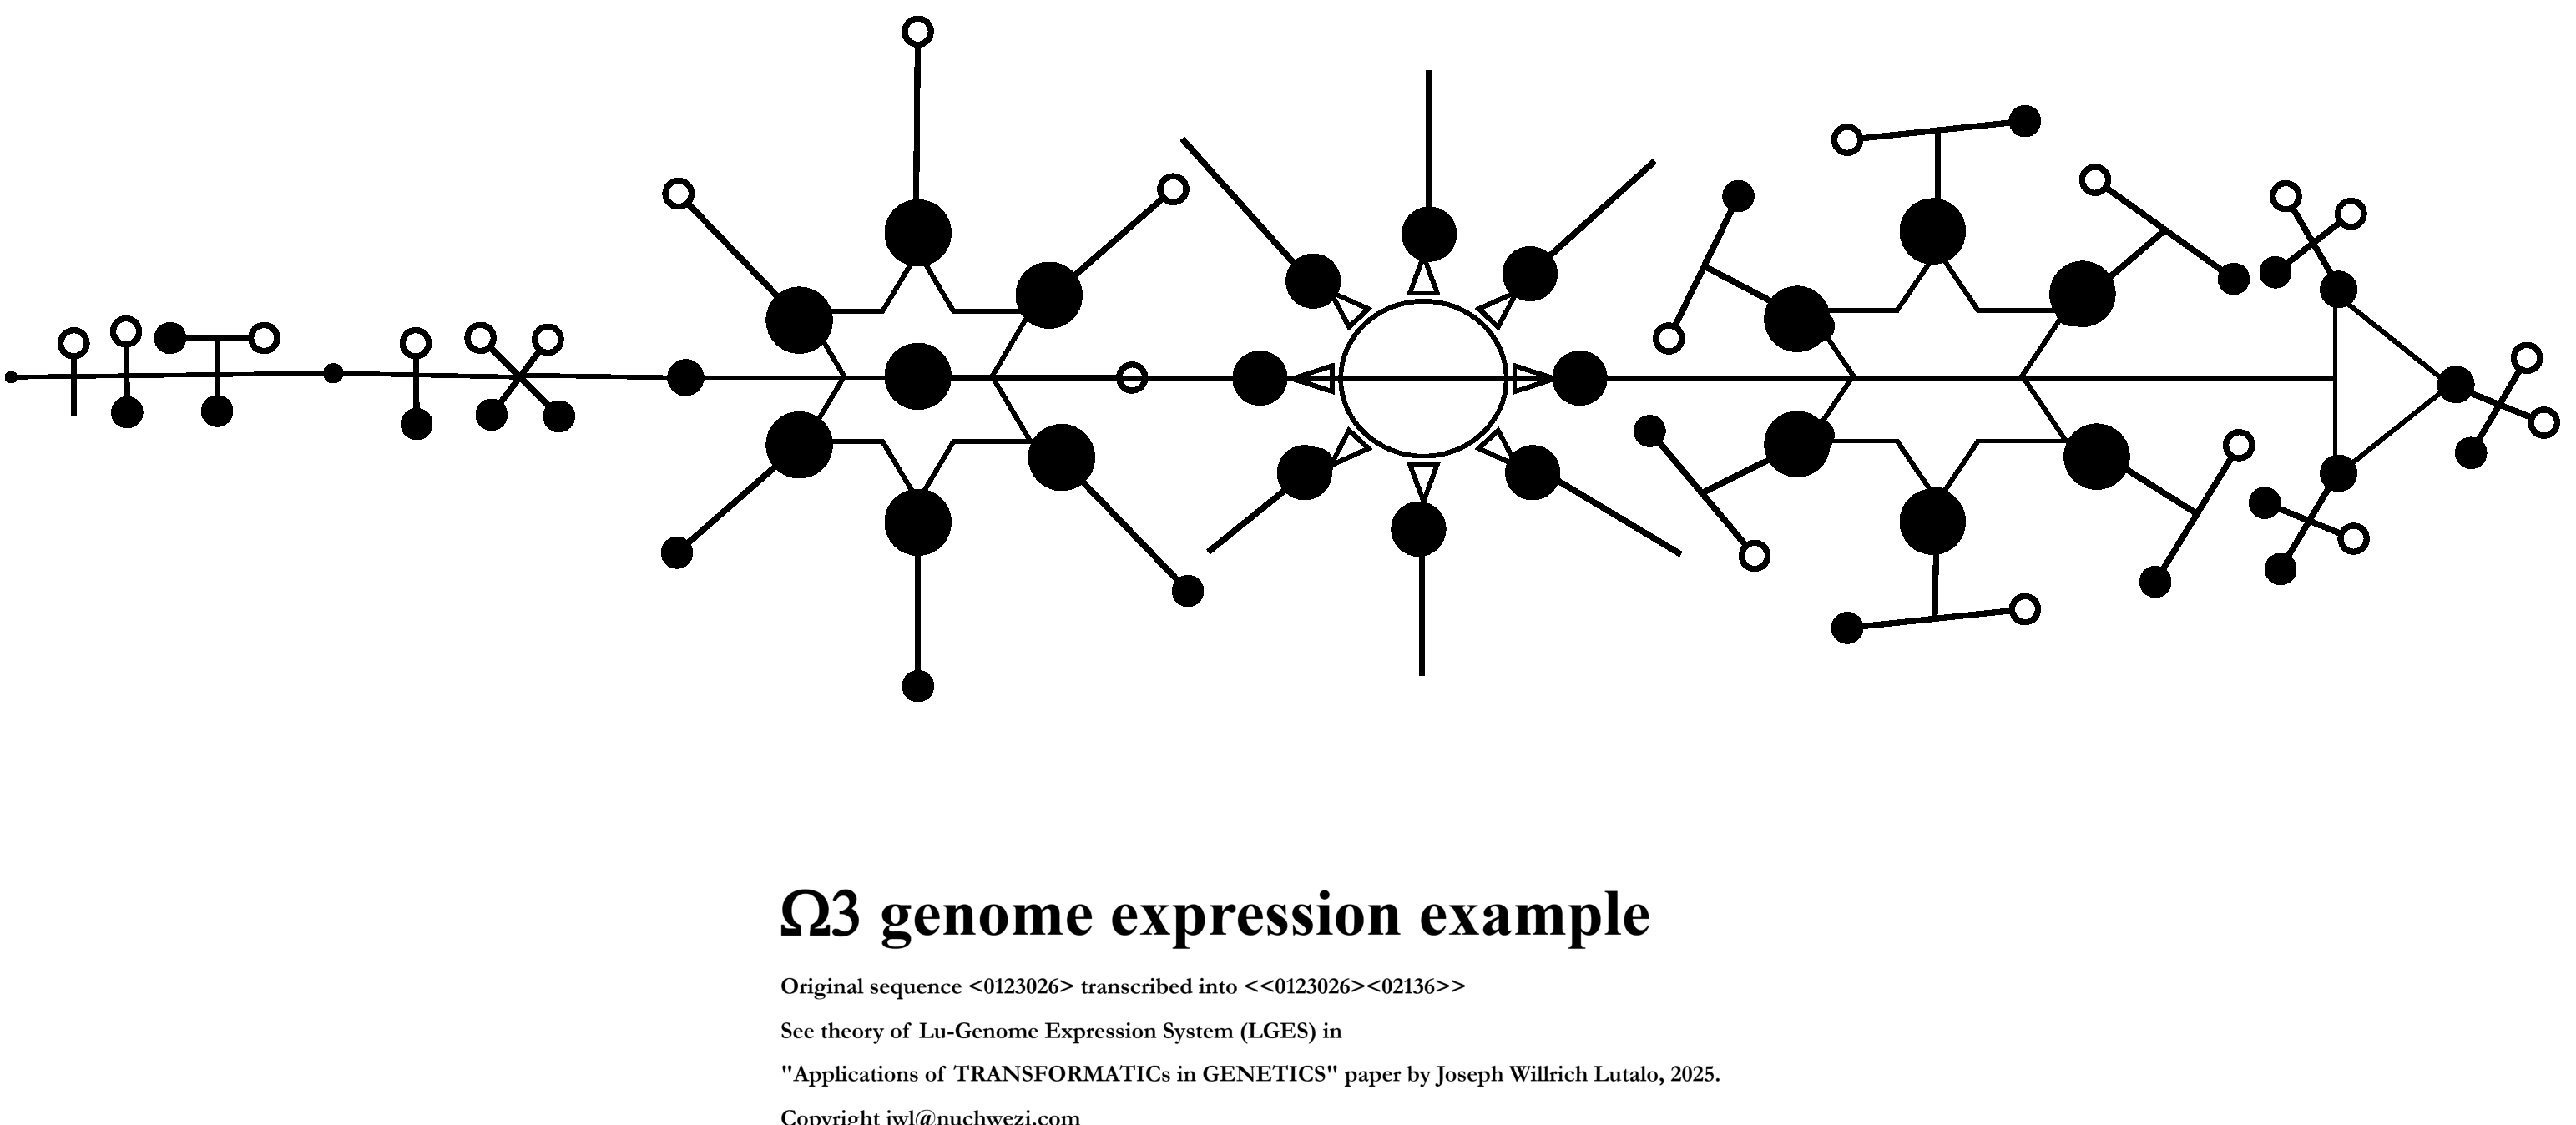
\includegraphics[trim=0cm 0cm 0cm 0cm, clip, width=0.9\textwidth,]{resources/pdfs/PLATONIC-EXA-landscape_ORIG.pdf}\\
   \caption{The equivalent LGES complete genome expression of the $\Omega_{3}$ genome sequence (from \textbf{Equation \ref{EQDNEXA}})}
  \label{FIGPLATONICEXA_ORIG}
  \end{center}
\end{figure}


Though we won't delve into exploring all kinds of possible \textit{interesting} scenarios with regards to the \textbf{LGES}, we can look at one other example and then move on. From the example hypothetical genome sequences we have encountered, perhaps let us revisit \textbf{\hyperref[EQDNAV]{Equation \ref{EQDNAV}}} and see what the \textbf{Euler Virus} might look like when fully expressed in our system.

So, note that we already did the first-leg of \textbf{\hyperref[ALGCOZINPLATO_ORIG]{Algorithm \ref{ALGCOZINPLATO_ORIG}}}, and have seen what the \textbf{FGE} prefix --- the \textbf{IFA}, would look like in \textbf{Figure \ref{FIGOZEVIRUS}} So, like we did for $\Omega_{3}$ in the last exploration, let us start by looking at what the numeral-equivalence of the processed $\Omega_{veuler}$ would be like. For brevity, we can sum up the entire production/transformation that leads to the complete \textbf{FGE} with correct prefix and suffix, and thus $\boxed{OZ(\Omega_{veuler})}^*$ as:

\begin{center}
\fbox{
\begin{minipage}{\textwidth}

\begin{trans}
\label{TRANSGENSEQEVIRUS_ORIG}
$\Omega_{veuler} = \langle 2,7,1,8,2,8,1,8 \rangle \rightarrow \hbar(\overset{>}{\Omega_{veuler}}) = \text{\textbf{8}3\textbf{2}2\textbf{1}2\textbf{7}1} \rightarrow \overset{>}{\Omega_{veuler}} = \langle 8, 2, 1, 7 \rangle \implies \boxed{OZ(\Omega_{veuler})} \approx \lnot{\langle 8, 2, 1, 7  \rangle_{pf}} \implies \boxed{OZ(\Omega_{veuler})}^* =  \langle 2,7,1,8,2,8,1,8 \rangle_{oz}\cdot\boxed{\langle 1, 7, 8, 2 \rangle}_{pf}$\\
\end{trans}

\end{minipage}}
\\
\end{center}


Note that in that derivation depicted in \textbf{\hyperref[TRANSGENSEQEVIRUS_ORIG]{Transformation \ref{TRANSGENSEQEVIRUS_ORIG}}}, one of the most tricky parts is computing that FGE suffix, $\boxed{OZ(\Omega_{veuler})}$, the \textbf{PFA} --- which is formalized/defined by \textit{especially}\footnote{\textbf{\hyperref[EQEXTFGEJOINTSUF_ORIG]{Equation \ref{EQEXTFGEJOINTSUF_ORIG}}} is what covers the special symbol `0', that is treated as a JOINT/GAP in the \textbf{PFA} and as STOP/GAP in \textbf{IFA}.} \textbf{\hyperref[EQFBOXED_ORIG]{Equation \ref{EQFBOXED_ORIG}}}. So, once that is done, and we have our final numeral-\textbf{FGE} as such:

\begin{equation}
\label{EQGFEEVIRUS_ORIG}
\boxed{OZ(\Omega_{veuler})}^* =  \langle 2,7,1,8,2,8,1,8 \rangle_{oz}\cdot\boxed{\langle 1, 7, 8, 2 \rangle}_{pf}
\end{equation}

Of course, concerning \textbf{\hyperref[EQGFEEVIRUS_ORIG]{Equation \ref{EQGFEEVIRUS_ORIG}}}, note that, or rather, keep in mind that concerning the \textbf{PFA} component, $\boxed{OZ(\Omega_{veuler})}$, the corresponding associated sequence in numeral form is the \textbf{IFA MSS}, $\overset{>}{OZ(\Omega_{veuler})} = \overset{>}{\Omega_{veuler}} = \langle 8, 2, 1, 7 \rangle$. And thus, using necessary transcription and translation ciphers as well as the multiplication rules required by \textbf{\hyperref[EQFBOXED_ORIG]{Equation \ref{EQFBOXED_ORIG}}} when treating of the \textbf{PFA}, we then generate the final genome expression for the \textbf{Euler Virus} under the \textbf{LGES} that looks as in \textbf{Figure \ref{FIGLGESEULERVIRUS_ORIG}}.


\begin{figure}[H]
  \begin{center}
  %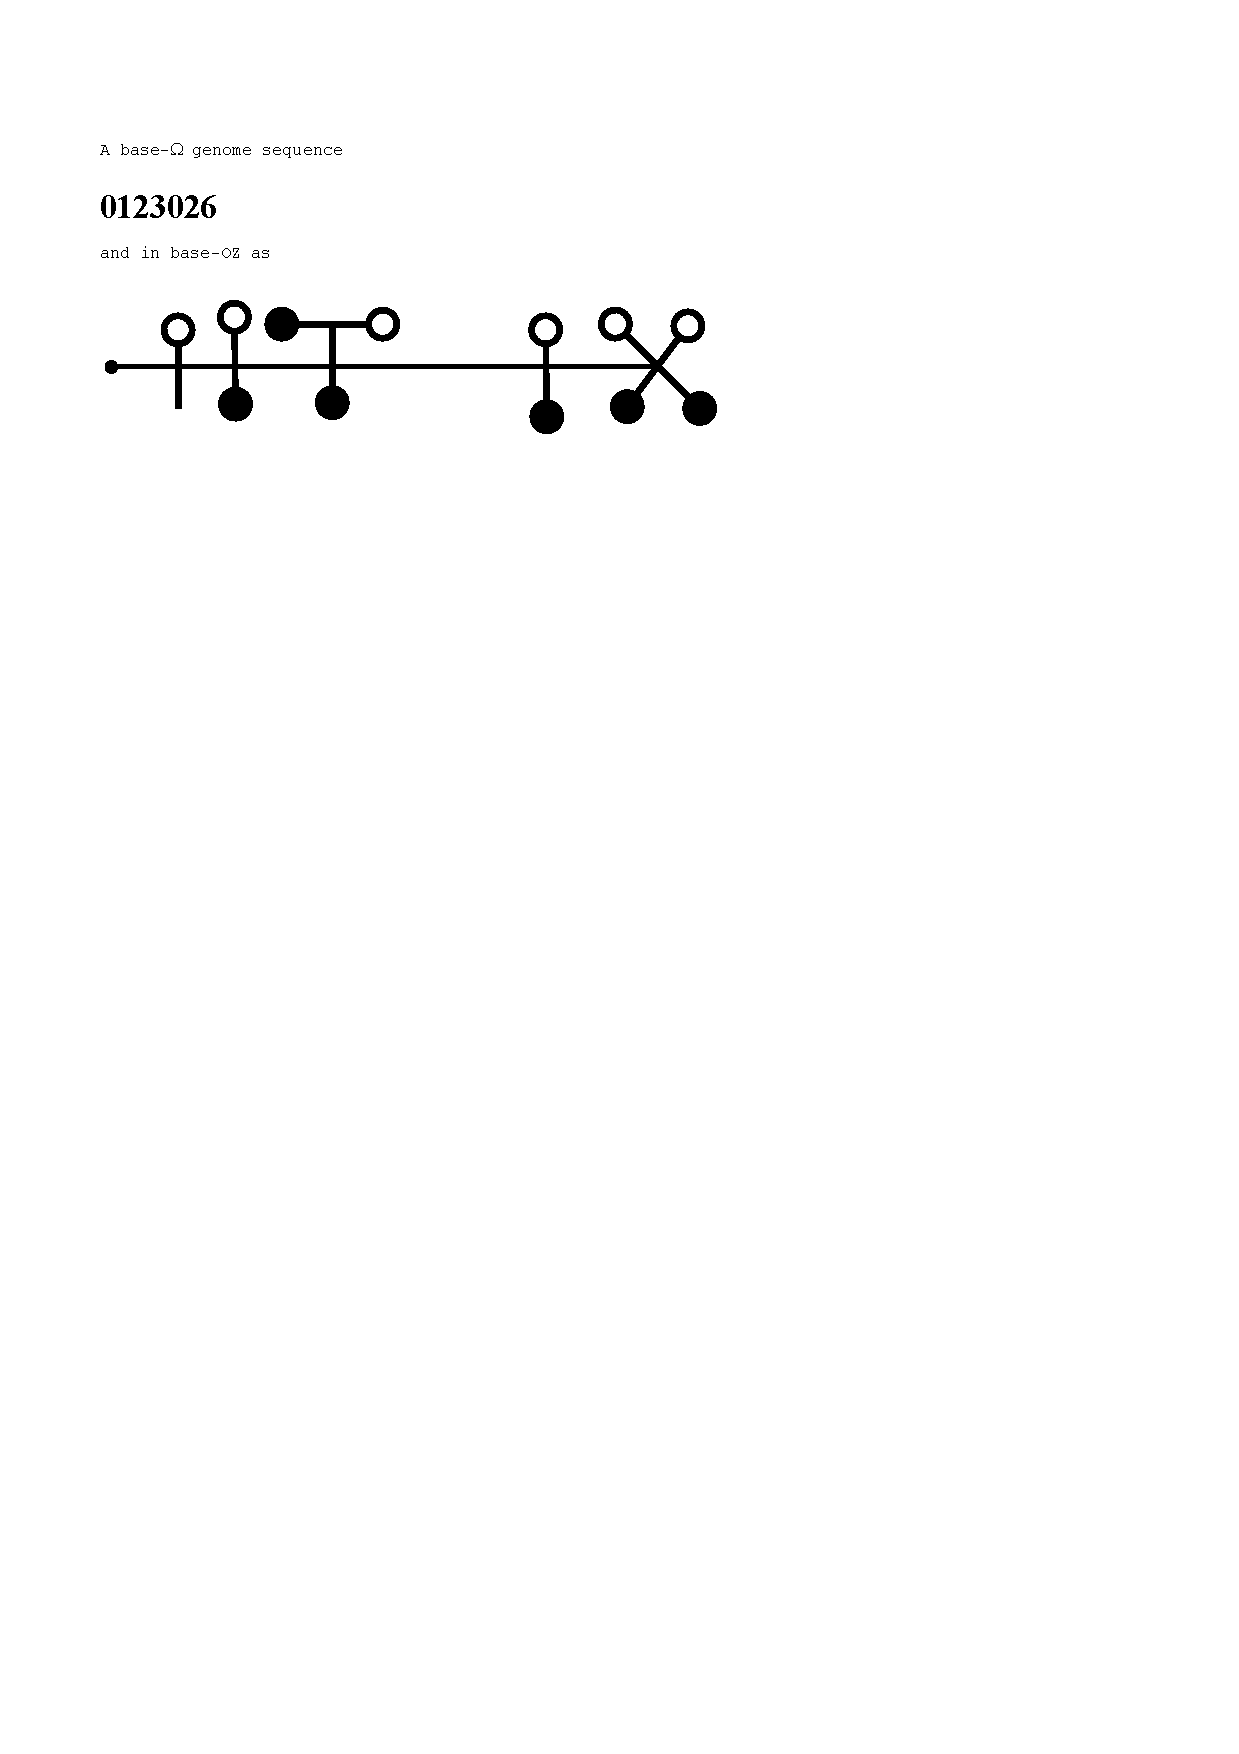
\includegraphics[trim=0cm 20cm 0cm 0cm, clip, width=0.9\textwidth,]{resources/pdfs/OZINCIPHER-APP3-EXA.pdf}\\
   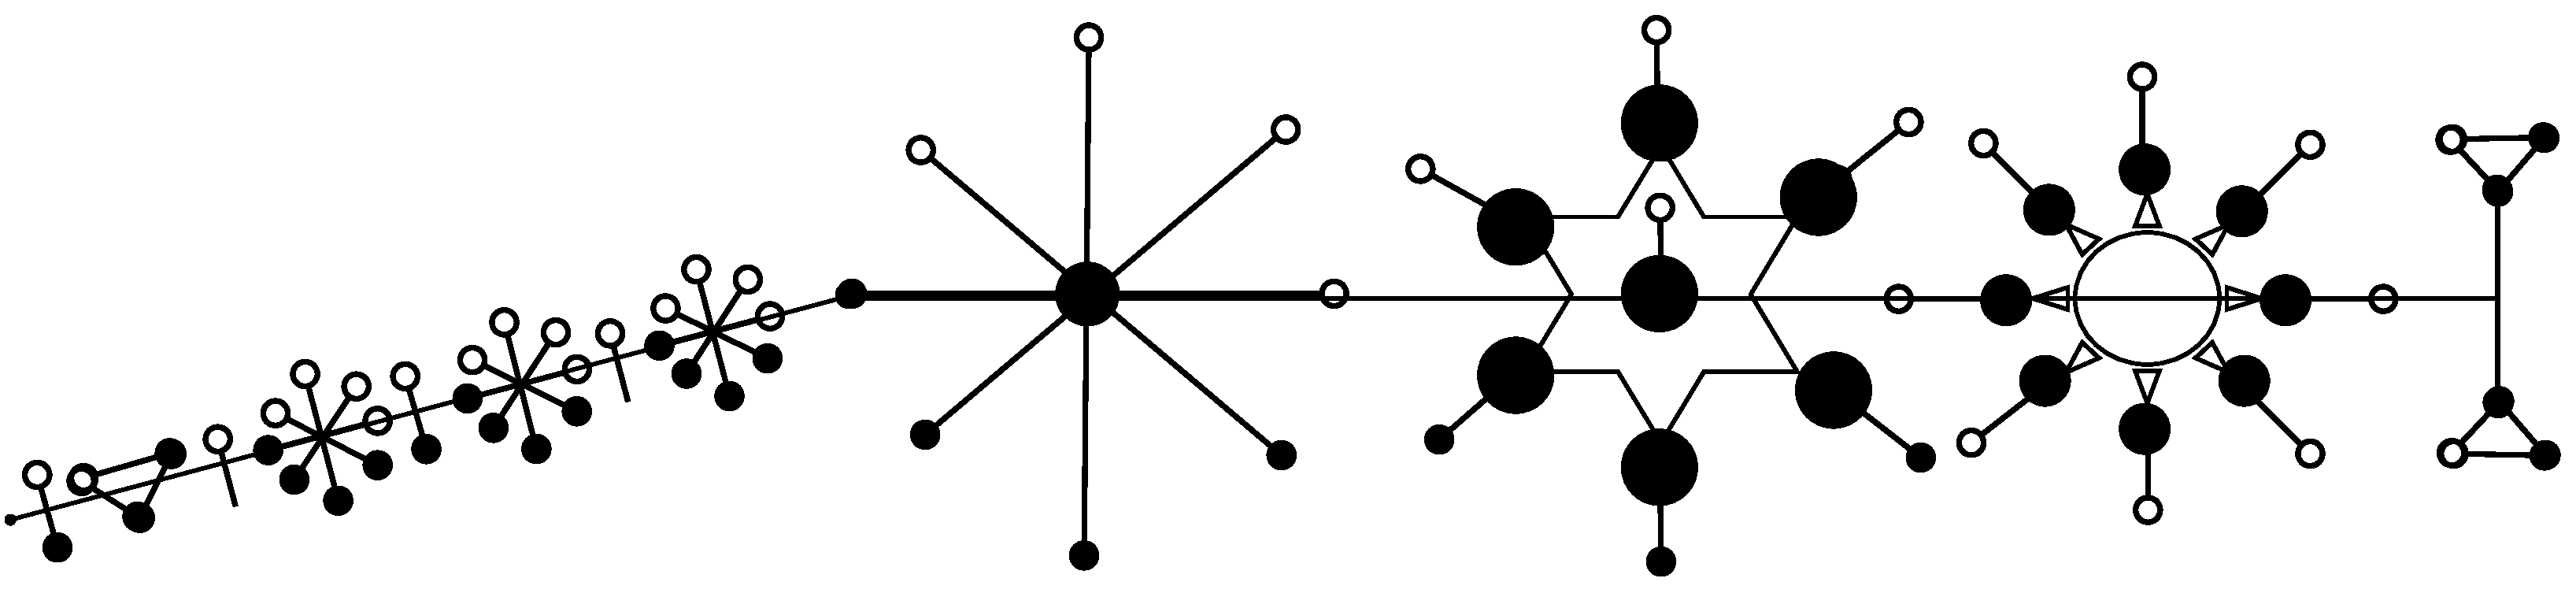
\includegraphics[trim=0cm 0cm 0cm 0cm, clip, width=0.9\textwidth,]{resources/pdfs/PLATONIC-EULERVIRUS-landscape_ORIG.pdf}\\
   \caption{The equivalent LGES complete genome expression of the $\Omega_{veuler}$ (Euler Virus) genome sequence (from \textbf{Equation \ref{EQGFEEVIRUS_ORIG}})}
  \label{FIGLGESEULERVIRUS_ORIG}
  \end{center}
\end{figure}


Now, concerning that rendering of the genome sequence expressed in \textbf{Equation \ref{EQGFEEVIRUS_ORIG}}, it might be worth noting that unlike the earlier examples of \textbf{LGES} expressions, we have taken the liberty to exploit that special joint that kick-starts the \textbf{PFA}, or rather, which separates the \textbf{IFA} from the \textbf{PFA} in a \textbf{FGE} expression. So, just like an organism with a physical joint might sometimes appear as angled or curved, so we have chosen to depict the $\Omega_{veuler}$ with its one joint\footnote{Definitely, and interesting to explore, a genome sequence with multiple JOINT points in it might be how an organism with say appendages such as legs, hands and a head that can move independently of the core/thorax of the body is possibly arrived at. The interested student should go ahead and explore more non-trivial $\Omega$-base sequences just to see what's possible.} well utilized. However, and important to note; it is not just joints that might appear different across different renderings of the same basis genome sequence. So, in \textbf{Figure \ref{FIGLGESEULERVIRUSv2_ORIG}}, we see another variation of the same sequence, with readily noticeable differences being the IFA-PFA joint in its neutral position, and then the second node in the PFA (corresponding to \textbf{$7_{pf} \otimes 2_{oz}$} or rather \textbf{$7_{pf} + 7 \times 2_{oz}$}) with the $2_{oz}$ appendages depicted mostly aligned horizontally.


\begin{figure}[H]
  \begin{center}
  %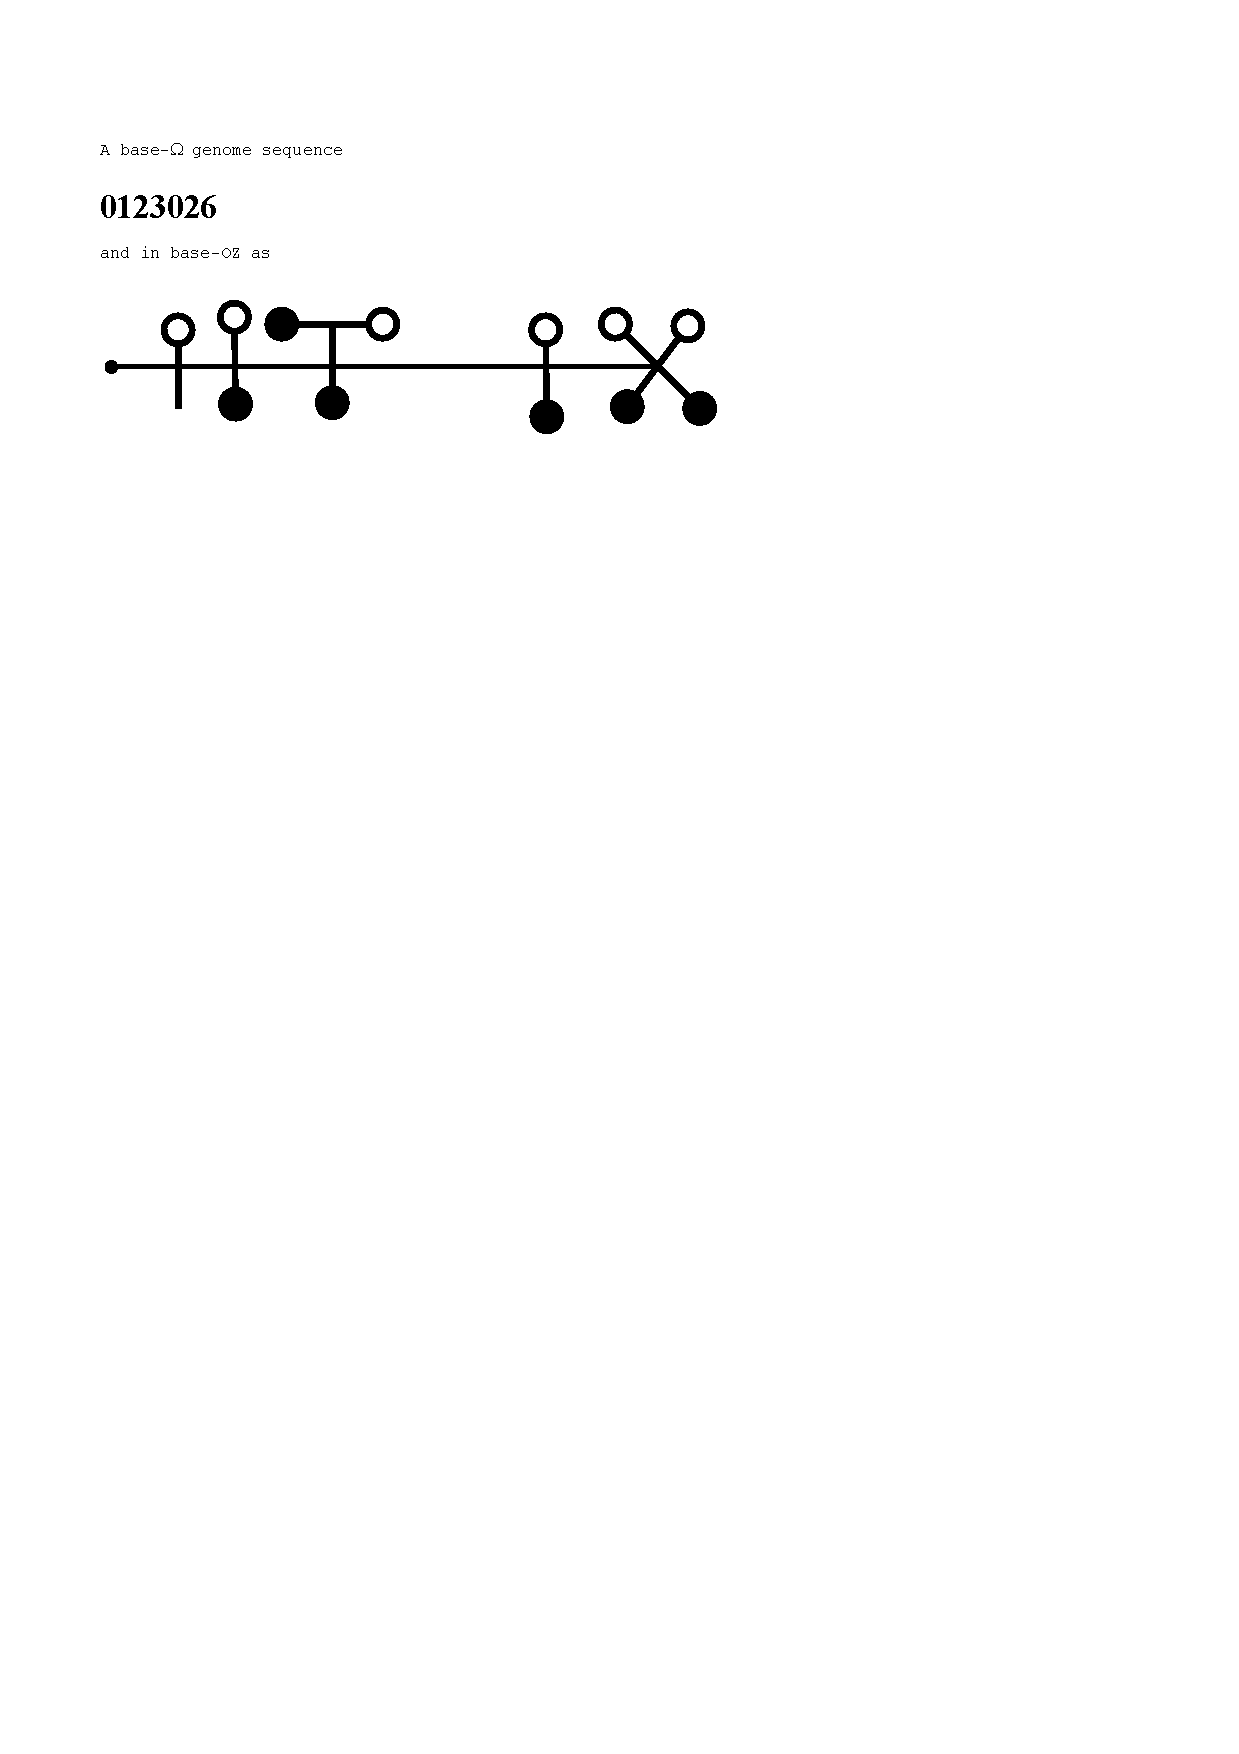
\includegraphics[trim=0cm 20cm 0cm 0cm, clip, width=0.9\textwidth,]{resources/pdfs/OZINCIPHER-APP3-EXA.pdf}\\
   \includegraphics[trim=0cm 0cm 0cm 0cm, clip, width=0.9\textwidth,]{resources/pdfs/v2-PLATONIC-EULERVIRUS-landscape_ORIG.pdf}\\
   \caption{The \textbf{alternative rendering}  of the same sequence as $\Omega_{veuler}$.}
  \label{FIGLGESEULERVIRUSv2_ORIG}
  \end{center}
\end{figure}

Concerning \textbf{Figure \ref{FIGLGESEULERVIRUSv2_ORIG}}, the alternative rendering  of the same sequence as $\Omega_{veuler}$ first depicted in \textbf{Figure \ref{FIGLGESEULERVIRUS_ORIG}}, we see that underlying the variations is how the \textit{degrees of freedom} in rendering the genome have somewhat been exploited. Notice how the joint and appendages are placed or oriented about the platonic forms that mostly remain unchanged across the two renderings --- except perhaps in scale. And talking of scaling nodes, in the future, we might want to explore whether in such a system as \textbf{LGES} in which the expression is sensitive to measures such as the \textbf{IFA MSS}, whether it might make sense to scale each subsequent pf-node in the \textbf{PFA} based on its position within the sequence? Though we didn't have such a rule included in \textbf{\hyperref[ALGCOZINPLATO_ORIG]{Algorithm \ref{ALGCOZINPLATO_ORIG}}}, and yet, our example renderings here have somewhat taken advantage of that plausible logic.

That said, note that we started this work with a photograph of a pineapple ready to harvest (see \textbf{Figure \ref{FIGPINEAPPLE}}), and though the associated discussion\footnote{Checkout video/mini-lecture on the matter at author's YouTube: \url{https://youtube.com/shorts/yTJzBEpw7Z4}} by the author did bring up the matter of how it might inspire a genome expression system in which the prefix is the actual DNA that renders the rest of the organism (fruit, plant-base and roots in this case of the pineapple), it is left as an exercise to the reader to decide whether example genome sequence expressions/renderings such as in \textbf{Figure \ref{FIGLGESEULERVIRUS_ORIG}} depict this pineapple-inspired philosophy.


\chapter{Future Directions and Explorations of TRANSFORMATICS in both PHYSICS and GENETICS?}


\begin{defn}[The Transformatics of \textbf{Teleportation}]

\begin{defn}[\textbf{Teleportation}] is a natural, simulated or preternatural phenomena, by which a collection of particles existing in some definite space and time, are projected to a derivative collection of similar particles, with one or more of their properties altered --- in case of conventional concepts of teleportation, such might mean expressing \textit{a thing} that is existing at the present time, as it were or shall be in either a past or future time frame respectively. In the language and calculus of transformatics, such would be a transformation of some given sequence of \textit{n}-grams of dimension 1 or more, where each particle is described by a set of 4 or more numeric values such as their $x$, $y$, $z$ coordinates in space, and a fourth coordinate, $t$, that captures the time at which that location is expressed. A teleportation machine then, is any abstract or \textit{actual} machine, which, when presented with the \textit{thing} --- say, a matrix of particles describing their initial location in some particular space-time, can then produce and return another matrix depicting how the initial space shall be at a later or earlier (basically, different) time, as per the following \textbf{time machine} specification:

\begin{defn}[The \textbf{Teleportation Machine}, M$\{\Delta T \rightarrow \Delta P\}$] 
is the machine, which, when given a sequence, $P^n\langle \rho_\alpha | \invpi(\rho) = 3+k \land \forall \rho_{ki} \in P : k \in \mathbb{N}, i \in [1,3] : \alpha = \frac{n}{3} \rangle$ such that $P^{2\alpha}$ is some derived resultant sequence of particles\footnote{Basically, coordinates in some \textbf{$\alpha-$space}, such that $\alpha = 3$ represents \textbf{3D} space for example. However, for the teleportation machine, we need to also cater for \textbf{the time property} of each particle in the sequence $P^{n\times k}$, and so, perhaps the minimal sequence dimensions required for the sequence of particles to be \textit{teleportable} is say $\alpha \implies dim \perp dim \geq 4 \quad \land \quad dim \leq \alpha = n \times k$.} of $3+k$ dimension, and so the machine can produce a new sequence of similar dimensions and/or same cardinality or greater, $P^*$,such that each particle $\rho$ in the original sequence has a complement or pairwise-partner particle, $\rho^*$, in the resultant sequence, $P^*$, as produced by the following sequence transformer that processes a source sequence so as to produce any correct resultant sequence as per the transformer specification:

\begin{transf}[The \textbf{Teleportation Transform}]
\label{TRANSFTELEP}
$P^{n} \rightarrow P^* ;$\\
$\invpi(P^*) = 2n : \forall \rho_i \in P^n \exists \rho^*_i \in P^* : \rho^*_i = \rho_i \quad \land \exists \rho^*_{i+n} : \tilde{A}(\rho_i \rightarrow \rho^*_{i+n}) > 0$\\
$\land \invpi(P^n) = n$\\
$\land \exists f(\rho_i,\Delta T) = \rho^*_{i+n}$
$\qed$
\end{transf}
\end{defn}

\end{defn}

With \textbf{\hyperref[TRANSFTELEP]{Transformer \ref{TRANSFTELEP}}}, and some time-sensitive translation function 

\begin{equation}
f({x,y,z,t_1,t_n}) = \Gamma(\delta x,\delta y,\delta z,\Delta T)
\end{equation}

We can predict/extrapolate any point or particle between two moments across space and time, relative to the absolute time change and a particular resolution space frame. Thus, and for example, we could take a plane and by translating it to another plane removed from the first by a reasonable significant distance, and such that the translation is orthogonal to some dimension $dim < 3 + k$, we might describe a solid --- a teleportation of particles too, formed by rotating the plane about some axis such as perpendicular to it, and such that the space-time thus spanned is bound by the source and resultant plane sequences, but also defined by them.

$\qed$
\end{defn}


Because this volume is about how we might apply transformatics in GENETICS, and yet the underlying \textit{original} intent was to also explore how to further transformatics as its own line of inquiry, not just in Genetics, but also in other sciences and perhaps even the arts(?), it shall make sense to add to what has already been discussed and shared in the rest of this book, with a sharing of a recent excerpt from the author's psychoanalytic notes --- because, like we mentioned in the preface of this work, Carl Jung's ideas\cite{jung1964symbols} on leveraging dream-analysis to further not just our understanding of ourselves but also of the world, did have such a great impact on the author over the years, it wouldn't make sense closing this book without sharing an aspect about how dreaming and Jung's methods have helped in making much of this work possible, as well as how it might help define the future directions of our further research and studies in relation to the current subject. 

Talking of which, the following is a verbatim excerpt, and is accompanied by a painting --- ``Arrival of the Anunnaki"\footnote{Image credit from author's Art Portfolio: \url{https://www.deviantart.com/nemesisfixx/art/Arrival-of-the-Anunnaki-inverted-942888530}}, also by the author, and part of their \textbf{Zermelo Frankael Dream Collection}\footnote{To get an idea what was in the other paintings in that collection from 2022, checkout \url{https://www.deviantart.com/nemesisfixx/art/The-Zermelo-Frankael-Dream-Collection-II-942887985} and \url{https://www.deviantart.com/nemesisfixx/art/Best-of-JWL-Art-from-2022-940119085}} most of whose art pieces have since been either sold or given out as souvenirs to friends and family.


\begin{figure}[H]
  \begin{center}
  %\includegraphics[trim=0cm 20cm 0cm 0cm, clip, width=0.9\textwidth,]{resources/pdfs/OZINCIPHER-APP3-EXA.pdf}\\
   \includegraphics[trim=0cm 0cm 0cm 0cm, clip, width=0.9\textwidth,]{resources/images/annunaki.jpg}\\
   \caption{The surreal painting, ``Arrival of the Anunnaki", by Joseph W. Lutalo, as part of their 2022 \textbf{The Zermelo Frankael Dream Collection} that was first exhibited at Ndugu Art Gallery then in Entebbe Town.}
  \label{FIGANNUNAKI}
  \end{center}
\end{figure}


\begin{center}
\fbox{
\begin{minipage}{\textwidth}


\texttt{In a dream, I have seen that I was somewhere in a laboratory with some very intelligent fellows and that we were exploring potential applications of TRANSFORMATICS in PHYSICS by conducting simulation experiments using a large hologram machine that looked like a table around which we sat and held discussions.}

\texttt{I saw that among interesting analyses we conducted was the matter of trying to understand ``The Bermuda Triangle Problem". In particular, we were simulating a strong magnetic field situated at the center of some location upon earth, and that if any flying object --- such as Flying Saucers (UFOs) attempted to fly close enough to this gravitating point, it would cause their trajectories to somewhat get warped towards the center, and so that, no matter how strong the tangential velocity of the craft was relative to the center of attraction at some moment with time T=tn, at any other later moment such that T=t(n+1), the centripetal force on the craft would be even stronger, and that the distance from the point of the center of attraction would be lesser at t(n+1) than at tn, and so that, eventually the craft would spiral down into the point and somewhat crash or (like for the case of the whirlpool-like Bermuda Triangle), get swallowed into some kind of black hole (in the ocean).}

\texttt{The simulations looked so realistic despite being generated by a super computer, and it felt like we were performing reconnaissance studies about aliens visiting Earth at say... Area 51! Then I woke up.
}


\#\#\# \textbf{A Dream About The Bermuda Triangle Experiment \& Applying TRANSFORMATICS in PHYSICS}

\end{minipage}}
\\
\end{center}

\large

\textbf{NOTE:} \textit{After waking up and thinking a bit about all this.. a stunning realization occurred to me; there's an acrylic painting I once did (titled ``Arrival of the Annunaki", and which I had exhibited at the then Ndugu Art Gallery in Entebbe Town circa 2022, but which now was at home with me), in which I painted a vision that had occurred to me concerning a spaceship that visited Earth some day (in the future perhaps), and that the ship shone a very brilliant light upon some village, and that as people freaked out, a ladder descended from the ship onto the earth, and some few bold people ascended into the ship by climbing up that ladder, while others, too afraid, only scattered and ran away.} 


\textit{So, while thinking about this Bermuda experiment on TRANSFORMATICS and also this interesting painting, and trying to connect the dots... I feel like.. perhaps there is something about the DNA ladder-like structure that could get us to understanding the biology or natural powers of aliens? Life on other planets or worlds perhaps? It strongly feels like these two ``dreams" might be telling us or pointing us towards something both alarming and exhilarating! Also, it could indeed inspire future directions and explorations of TRANSFORMATICS in both PHYSICS and GENETICS!}


\textit{\#dream \#diary \#advanced \#physics \#transformatics \#jwl \#reflections \#futuredirections
\#CREATED:Aug 22, 2025 03:02:32}

\Large

%-------[ END CONTENT ]


\end{appendices}

\includepdf[pages=1]{resources/pdfs/note_cover.pdf}

\bibliographystyle{unsrt}
\bibliography{references}

%\comment{

%\newpage

\vspace{5cm}
\fbox{
\begin{minipage}{0.9\textwidth}
\textbf{TO CITE:}\\

Lutalo, Joseph Willrich (2025). \textbf{Applying TRANSFORMATICS in GENETICS} I*POW. Preprint. \url{https://doi.org/10.6084/m9.figshare.29941127}

\end{minipage}}
\\
%}


%---[ END BOOK END/BACKCOVER]

\chapter*{Colophon}
\addcontentsline{toc}{chapter}{Colophon}


\texttt{COVER-ART:} \textbf{J. Willrich Lutalo}, as prompt engineer, using \textbf{Microsoft Bing Image Creator}, powered by DALL$-$E.


\texttt{GRAPHICS:} \textbf{Adobe Express} on Android.


\texttt{PRIMARY-EDITOR:} \textbf{TexMaker} v6.0.0 using \textbf{LaTeX} on Microsoft Windows v10.


\texttt{REFERENCE-MANAGER:} \textbf{BibTeX} v0.99d (package manager: MiKTeX v24.4).


\texttt{SECONDARY-EDITOR:} \textbf{VIM}, Vi IMproved v8.2 text editor, via \textbf{WSL}.


\texttt{PUBLISHER:} \textbf{I*POW} \url{https://t.me/ipowriters}


\texttt{FONT:} \textbf{Computer Modern Roman}

% insert [back] cover --- could just be a PNG or PDF
\includepdf[pages=1]{resources/pdfs/back_cover.pdf}

\end{document}
